\documentclass[oneside]{book}

%%%%%%%%%%%%%%%%%%%%%%%%%%%%%%Paquetes%%%%%%%%%%%%%%%%%%%%%%%%%%%%%%%%%%%%%%%%%%%%%%%5
%%%%%%%%%%%%%%%%%%%%%%%%%%%%%%%%%%%%%%%%%%%%%%%%%%%%%%%%%%%%%%%%%%%%%%%%%%%%%%%%%%%%%
\usepackage{empheq}
\usepackage[spanish]{babel}
%\usepackage[utf8]{inputenc}
%\usepackage[T1]{fontenc}
\usepackage{amssymb,amsmath,amsthm}
\usepackage{enumerate}
\usepackage{verbatim}
\usepackage{ esint }
\usepackage{pst-all}
%\usepackage{pstricks-add}
\usepackage{array}
\usepackage{animate}
\usepackage{xparse}
\usepackage{listings}
\usepackage{ wasysym }
\usepackage{yfonts,mathrsfs,eufrak}
\usepackage{hyperref}
\usepackage{color}
\usepackage{url}
\usepackage{theorem}
\usepackage{boiboites}
\usepackage{wrapfig}
\usepackage[spanish]{varioref}
\usepackage{fontspec}
\usepackage[a4paper,driver=xetex,top=2.5cm, bottom=2.7cm,%
layouthoffset=10mm, left=2.3cm, right=6.2cm]{geometry}
\usepackage{pst-barcode}
\usepackage{fancyhdr}
\usepackage{marginnote}
 \usepackage{titlesec}
%%%%%%%%%%%%%%  Configuración página
\usepackage{natbib}
\usepackage{chapterbib}
\usepackage{fontawesome}
\usepackage{xcolor}
\usepackage{appendix}
\usepackage{chngcntr}
\usepackage{etoolbox}
\usepackage{lipsum}
\usepackage{mathtools}
\usepackage{csquotes}
%\usepackage{pstricks-add}
\usepackage{sagetex}
%\usepackage{sympytex}


\fancyfoot{}
\fancyhead[RO,LE]{\thepage}
\fancyhead[LO]{\leftmark}
\fancyhead[RE]{\rightmark}


\titleformat{\section}
  {\normalfont\Large\bfseries}{\thesection}{1em}{}[{\titlerule[0.8pt]}]

\AtBeginEnvironment{subappendices}{%
\chapter*{Apéndices}
\addcontentsline{toc}{chapter}{Apéndices}
\counterwithin{figure}{section}
\counterwithin{table}{section}
}

%%%%%%%%%%%%%%%%%%%%%%%%Colores
%Sugeridos por CEPEIPER
% \definecolor{color1}{rgb}{0.24,0.45,0.42}
% \definecolor{color2}{rgb}{0.44,0.62,0.42}
% \definecolor{color3}{rgb}{0.28, 0.51, .68}
% \definecolor{color4}{rgb}{0.29,0.3,0.57}
% \definecolor{color5}{rgb}{0.7,0.24,0.24}
% \definecolor{color6}{rgb}{0.72,0.4,0.28}
% \definecolor{color7}{rgb}{0.84,0.66,0.21}
% \definecolor{color8}{rgb}{0.3,0.29,0.28}


\definecolor{color1}{rgb}{0.48,0.89,0.84}
\definecolor{color2}{rgb}{0.48,0.89,0.84}
\definecolor{color3}{rgb}{0.28, 0.51, .68}
\definecolor{color4}{rgb}{0.29,0.3,0.57}
\definecolor{color5}{rgb}{0.7,0.24,0.24}
\definecolor{color6}{rgb}{0.72,0.4,0.28}
\definecolor{color7}{rgb}{0.84,0.66,0.21}
\definecolor{color8}{HTML}{8E87C1}


%%%%%%%%%%%%%%%%%%%%%% Configuracion listing

\lstset{ %
  backgroundcolor=\color{white},   % choose the background color; you must add \usepackage{color} or \usepackage{xcolor}
  basicstyle=\footnotesize,        % the size of the fonts that are used for the code
  breakatwhitespace=false,         % sets if automatic breaks should only happen at whitespace
  breaklines=true,                 % sets automatic line breaking
  captionpos=b,                    % sets the caption-position to bottom
  commentstyle=\color{color2},    % comment style
  deletekeywords={...},            % if you want to delete keywords from the given language
  escapeinside={\%*}{*)},          % if you want to add LaTeX within your code
  extendedchars=true,              % lets you use non-ASCII characters; for 8-bits encodings only, does not work with UTF-8
  frame=single,	                   % adds a frame around the code
  keepspaces=true,                 % keeps spaces in text, useful for keeping indentation of code (possibly needs columns=flexible)
  keywordstyle=\color{blue},       % keyword style
  language=Python,                 % the language of the code
  otherkeywords={symbols,dsolve,solve,Eq, simplify, subs, plot,Function},           % if you want to add more keywords to the set
  numbers=left,                    % where to put the line-numbers; possible values are (none, left, right)
  numbersep=5pt,                   % how far the line-numbers are from the code
  numberstyle=\tiny\color{color3}, % the style that is used for the line-numbers
  rulecolor=\color{black},         % if not set, the frame-color may be changed on line-breaks within not-black text (e.g. comments (green here))
  showspaces=false,                % show spaces everywhere adding particular underscores; it overrides 'showstringspaces'
  showstringspaces=false,          % underline spaces within strings only
  showtabs=false,                  % show tabs within strings adding particular underscores
  stepnumber=2,                    % the step between two line-numbers. If it's 1, each line will be numbered
  stringstyle=\color{color4},     % string literal style
  tabsize=2,	                   % sets default tabsize to 2 spaces
  title=\lstname                   % show the filename of files included with \lstinputlisting; also try caption instead of title
}

\lstdefinelanguage{GAP}{%
  morekeywords={%
    Assert,Info,IsBound,QUIT,%
    TryNextMethod,Unbind,and,break,%
    continue,do,elif,%
    else,end,false,fi,for,%
    function,if,in,local,%
    mod,not,od,or,%
    quit,rec,repeat,return,%
    then,true,until,while,SymmetricGroup,Elements,Subgroup,IsNormal,FactorGroup,>gap%
  },%
  sensitive,%
  morecomment=[l]\#,%
  morestring=[b]",%
  morestring=[b]',%
}[keywords,comments,strings]

%%%%%%%%%%%%%Configuración de fuente para XeLaTeX

%\setsansfont{Roboto Condensed}
\setsansfont{Gentium Basic}

\renewcommand{\familydefault}{\sfdefault}


%\renewcommand{\section}[1]{\section{#1}}


%%%%%%%%%%%%%%%%%%%%%%%%%%Nuevos comandos entornos%%%%%%%%%%%%%%%%%%%%%%%%%%%%%%%%
%%%%%%%%%%%%%%%%%%%%%%%%%%%%%%%%%%%%%%%%%%%%%%%%%%%%%%%%%%%%%%%%%%%%%%%%
\newenvironment{demo}{\noindent\emph{Dem.}}{$\square$ \newline\vspace{5pt}}

\newcommand{\com}{\mathbb{C}}
\newcommand{\dis}{\mathbb{D}}
\newcommand{\rr}{\mathbb{R}}
\newcommand{\oo}{\mathcal{O}}
\newcommand{\der}[2]{\frac{\partial #1}{\partial #2}}
\renewcommand{\v}[1]{\overrightarrow{#1}}
\renewcommand{\epsilon}{\varepsilon}
\newcommand{\p}{\varphi}
\renewcommand{\b}[1]{\boldsymbol{#1}}
\renewenvironment{frame}[1]{}{}
\newcommand{\link}{\reversemarginpar\marginnote{%\fontsize{24}{24                                                                                                                                                                                                                                                                                                                                                                                                                                                                                                                                                                                                                                                                                                                                                                                                                                                                                                                                                                       
%}\selectfont
\faExternalLink} %
\normalmarginpar
}
\newcommand{\advertencia}{\reversemarginpar\marginnote{%\fontsize{11}{11}\selectfont
\faBolt}%
\normalmarginpar }
\newcommand{\lectura}{\reversemarginpar\marginnote{%\fontsize{11}{11}\selectfont
\faBook}%
\normalmarginpar}
\newcommand{\actividad}{\reversemarginpar\marginnote{%\fontsize{11}{11}\selectfont
\faCogs}%
\normalmarginpar}

%\renewcommand{\lim}{displaystyle\lim}
\DeclareMathOperator{\atan2}{atan2}
\DeclareMathOperator{\sen}{sen}



%%%%%%%%%%Definimos una caja con color
\newlength\mytemplen
\newsavebox\mytempbox
\makeatletter
\newcommand\mybluebox{%
\@ifnextchar[%]
{\@mybluebox}%
{\@mybluebox[0pt]}}
\def\@mybluebox[#1]{%
\@ifnextchar[%]
{\@@mybluebox[#1]}%
{\@@mybluebox[#1][0pt]}}
\def\@@mybluebox[#1][#2]#3{
\sbox\mytempbox{#3}%
\mytemplen\ht\mytempbox
\advance\mytemplen #1\relax
\ht\mytempbox\mytemplen
\mytemplen\dp\mytempbox
\advance\mytemplen #2\relax
\dp\mytempbox\mytemplen
\colorbox{color1}{\hspace{1em}\usebox{\mytempbox}\hspace{1em}}}
\makeatother
\DeclareDocumentCommand\boxedeq{ m g }{%
{\begin{empheq}[box={\mybluebox[2pt][2pt]}]{equation}% #1%
\IfNoValueF {#2} {\label{#2}}%
#1
\end{empheq}
}%
}


%%%%%%%%%%%%%%%%%%
\newboxedtheorem[boxcolor=color1, background=color2, titlebackground=color1,
titleboxcolor = black,thcounter=section]{problema}{Problema}{thcounter1}

\newboxedtheorem[boxcolor=color1, background=color2, titlebackground=color1,
titleboxcolor = black,thcounter=section]{teorema}{Teorema}{thcounter2}

\newboxedtheorem[boxcolor=color1, background=color2, titlebackground=color1,
titleboxcolor = black,thcounter=section]{definicion}{Definici\'on}{thcounter3}

\newboxedtheorem[boxcolor=color1, background=color2, titlebackground=color1,
titleboxcolor = black,thcounter=section]{lema}{Lema}{thcounter4}

\newboxedtheorem[boxcolor=color1, background=color2, titlebackground=color1,
titleboxcolor = black,thcounter=section]{corolario}{Corolario}{thcounter5}

\newboxedtheorem[boxcolor=color1, background=color2, titlebackground=color1,
titleboxcolor = black,thcounter=section]{proposicion}{Proposici\'on}{thcounter6}

\newboxedtheorem[boxcolor=color1, background=color2, titlebackground=color1,
titleboxcolor = black,thcounter=section]{codigo}{Función SymPy}{}

\newboxedtheorem[boxcolor=color1, background=color2, titlebackground=color1,
titleboxcolor = black,thcounter=section]{ejercicio}{Ejercicio}{}





\newcounter{ejemplo_cont}[chapter]
\setcounter{ejemplo_cont}{1}

% \makeatletter
% \@addtoreset{ejemplo_cont}{chapter}
% \makeatother

\newenvironment{ejemplo}{\noindent\textbf{Ejemplo  \arabic{chapter}.\arabic{ejemplo_cont}.} }{\addtocounter{ejemplo_cont}{1}}



%%%%%%%%%%%%%%%%%%%%%%%%%%%%%%%%%%%%%%%%%%%%%%%%%%%%%%%%%%%%%%%%%%%%%%%%%%%%%%%%%%%%%%%%%%%%%%%%%%%%%%%%%%%
%%%%%%%%%%Para escibir en clase articulo o similar









\title{Ecuaciones Diferenciales}
%\subtitle{Una Aproximación Teórica y Computacinal }
\author{Fernando Mazzone}

%%%%%%%%%%%%%%%%%%%%%%%%%%%%%%%%%%%%%%%%%%%%%%%%%%%%%%%%%%%%%%%%%%%%%%%%%%%%%%%%%%%%%%


\begin{document}




\renewcommand{\lim}{\mathop{\rm lím}}
\renewcommand{\inf}{\mathop{\rm ínf}}
\renewcommand{\liminf}{\mathop{\rm líminf}}
\renewcommand{\limsup}{\mathop{\rm límsup}}
\renewcommand{\min}{\mathop{\rm mín}}
\renewcommand{\max}{\mathop{\rm máx}}
\fontsize{11pt}{11pt}\selectfont

\pagestyle{fancy}
 
 
 \maketitle
 \tableofcontents
%   

% 
\chapter*{Prólogo}
\section{Sobre esta materia}

\begin{itemize}
 \item  \href{https://docs.google.com/viewer?a=v&pid=sites&srcid=ZGVmYXVsdGRvbWFpbnxlY3VhY2lvbmVzZGlmZXJlbmNpYWxldW5yY3xneDoyZjE0YzJmMDcyODc0ZGQ3}{Programa analítico.}
 \item  \href{https://sites.google.com/site/ecuacionesdiferencialeunrc/ecuaciones-diferenciales-unrc}{Página web} de la materia
 \item  Vamos a hacer uso intensivo de paquetes de matemática basados en \href{https://www.python.org/}{Python}, por ejemplo \href{http://www.scipy.org/}{SciPy},  \href{http://www.scipy.org/}{SymPy} y \href{http://www.sagemath.org/}{SAGE}.
 \item  Requeriremos muchos contenidos de la asignatura Física.
 \item  \begin{tabular}{m{4cm} m{2cm} m{2cm}} Bibliografía principal & 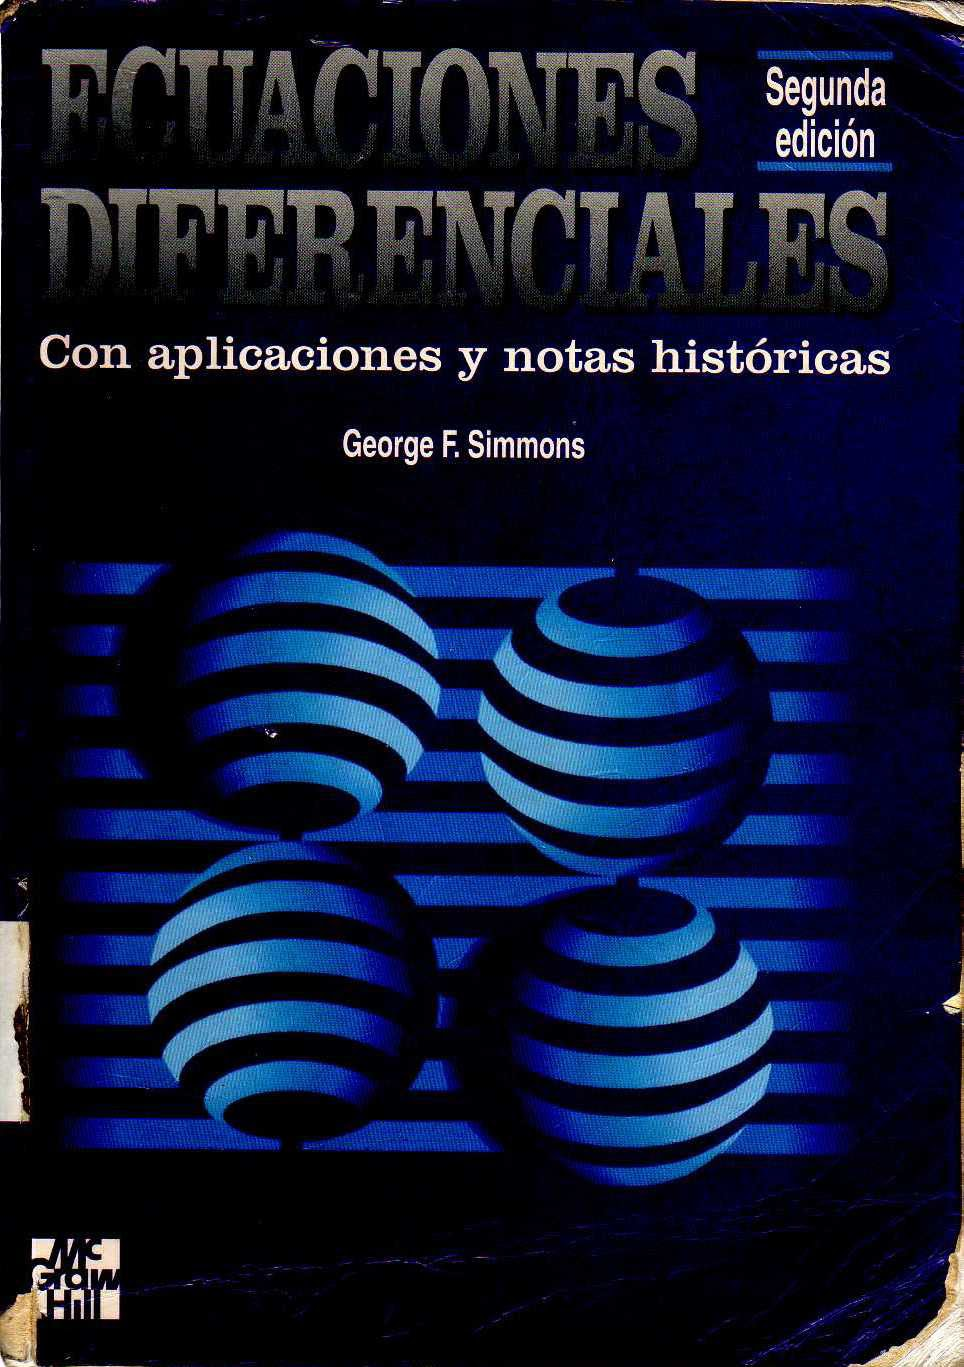
\includegraphics[scale=0.05]{imagenes/Tapa_Simmons.jpg} &    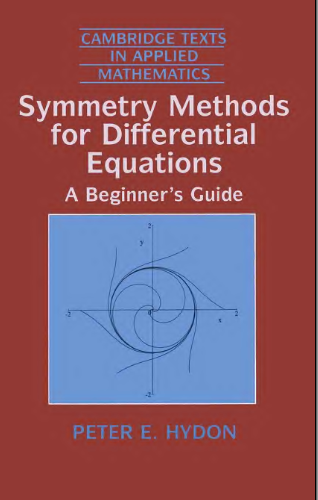
\includegraphics[scale=0.13]{imagenes/tapa_hydon.png}          \end{tabular}

\end{itemize}


% 
\chapter{Breve introducci\'on a Python y SymPy}


  Se trata de una masa puntual $m$ suspendida de un punto por medio de una barra de longitud $l$
 a la que suponemos sin masa. Equivale al movimiento sobre una guía circular.  Usaremos el ángulo $\alpha$ marcado en la figura, como variable dependiente.


\section{Descripción}
\href{https://www.python.org/}{Python} es un lenguaje de programación interpretado, 
abierto, facil de aprender, potente y portátil. Es utilizado en proyectos de todo tipo, 
no sólo aplicaciones científicas.
\marginpar{
%\begin{tabular}{b{.7in} b{.7in}}
 
\includegraphics[scale=.25]{imagenes/python-logo.png}
% &\begin{pspicture}(.7in,.7in)
%        \psbarcode{https://www.python.org/}{}{qrcode}
%    \end{pspicture}\\
%    &
% {\tiny https://www.python.org/}
% \end{tabular}
}



\href{http://www.scipy.org/}{SciPy}, 
Python científico, es un conjunto de módulos de python para distintos tipos de cálculos. 
Está integrado por los módulos, SymPy (para cálculos simbólicos), 
numpy (cálculos numéricos), matplotlib (gráficos) entre otros.  
En este curso sólo usaremos SymPy.
\marginpar{
%\begin{tabular}{b{.7in} b{.7in}}
 
\includegraphics[scale=.75]{imagenes/scipy_logo.png}
%&\begin{pspicture}(.7in,.7in)
%       \psbarcode{http://www.scipy.org/}{}{qrcode}
%   \end{pspicture}\\
%   &
%{\tiny http://www.scipy.org/}
%\end{tabular}
}


\href{http://www.sympy.org/}{SymPy}
es una biblioteca de Python para matemática simbólica. Su objetivo es convertirse en 
un sistema de álgebra computacional (SAC) completo, manteniendo el código lo más simple 
posible para que sea comprensible y fácilmente extensible. SymPy está escrito enteramente 
en Python y no requiere de ninguna biblioteca externa.
\marginpar{
 % \begin{tabular}{b{.7in} b{.7in}}
    
\includegraphics[scale=.25]{imagenes/sympy_logo.png}
% 	&
% 	  \begin{pspicture}(.7in,.7in)
% 	    \psbarcode{http://www.sympy.org/}{}{qrcode}
% 	  \end{pspicture}
% \\
% 	&
% 	  {\tiny http://www.sympy.org/}
%   \end{tabular}
}
% 
% 


% 
% \section{Local y online} 
% 
% Se pueden usar todos los recursos anteriores de dos formas
% \begin{enumerate}
% \item Instalando el software necesario en una computadora. Nos referiremos a este modo como de acceso local.
% 
% \item A traves de trasacciones en línea que permiten usar una computadora remota que ejecuta las instrucciones y programas que se tipean en una página web con la que se interactúa usualmente por medio de un navegador.  Hay varios sitios que ofrecen este servicio. 
%Sugerimos la \href{https://cloud.sagemath.com/}{SageMathCloud}. El usuario debe registrase.
% \end{enumerate}
% 


\section{Instalación}


Son muchas las componentes requeridas para poder ejecutar los programas con los que trabajaremos 
en esta asignatura. Hay que instalar un interprete de python, los módulos que utilizaremos 
(sympy, matplotlib), es útil utilizar entornos integrados de desarrollo (IDE), que facilitan al usuario
editores de código fuente (especializados con la sintáxis de python), consolas de comandos 
mejoradas (ipython, qt, etc). Otro recurso que se dispone son las notebooks, de las cuales 
hablaremos más adelante. Sería engorroso instalar todas estas componentes, que muchas veces 
tienen orígenes en desarrolladores diferentes, de manera independiente. Para nuestra fortuna
existen, las así llamadas, \emph{distribuciones}. Estas son programas que instalan todas 
las coponentes necesarias, o al menos muchas  de ellas, de un determinado paquete de software.
Recomendamos las siguientes distribuciones.  

\subsection{\href{https://www.continuum.io/downloads}{Anaconda}} 
La versión de código abierto de Anaconda es una distribución de alto rendimiento de Python y R 
e incluye más de 100 de los paquetes científicos más populares asociados a estos lenguajes.
%\reversemarginpar\marginpar{
\includegraphics[scale=.12]{imagenes/library.png} } 
Además, se puede acceder a más de 720 paquetes que pueden ser fácilmente instalados con Conda, 
 un programa incluído en Anaconda para la gestión de paquetes.
 Anaconda tiene licencia BSD que da permiso para utilizar Anaconda comercialmente 
 y para su redistribución. Al día que se escriben estas líneas, anaconda parece la opción más 
 sencilla y completa para instalar todos los recursos para desarrollar los contenidos de 
 estas notas. Existen versiones para linux, OS X y Windows. 
\marginpar{
    
\includegraphics[scale=.3]{imagenes/anaconda.png}
}

 Hay distribuciones específicas para distintos sistemas operativos

\subsection{Windows} La distribución  \href{https://code.google.com/p/pythonxy/}{python(x,y)}  instala el interprete de python y todos los módulos de scipy. Además el entorno de desarrollo integrado (IDE) spyder.
\marginpar{
\includegraphics[scale=.07]{imagenes/windows-logo.png}}


\subsection{linux} Aquí todo es más sencillo, el interprete de python suele venir con 
la distribución del SO y se pueden instalar los módulos, SymPy, NumPy, etc, 
recurriendo al administrador de paquetes o tipeando la sentencia adecuada en la línea 
de comandos.  
\marginpar{
\includegraphics[scale=.4]{imagenes/linux.jpeg}}

\subsection{Android} \href{http://qpython.com/}{Qpython} es una aplicación que permite ejecutar código python y una versión básica de sympy desde tablets y smartphones. Se descarga desde la plataforma \href{https://play.google.com/store/apps/details?id=com.hipipal.qpyplus}{google play}.
\marginpar{
\includegraphics[scale=.1]{imagenes/android.jpg}}

\subsection{Otros recursos de utilidad:} 

\href{http://www.sagemath.org/}{SageMath}  es un sistema de software
de matemáticas, libre, de código abierto bajo la licencia GPL. 
Es construído sobre  muchos paquetes de código abierto existentes: 
NumPy, SciPy, matplotlib, SymPy, Maxima, GAP, FLINT, R y muchos más.
Se acceda a su poder combinado a través de un lenguaje común, basado en Python.
\marginpar{
% \begin{tabular}{b{.7in} b{.7in}}

\includegraphics[scale=.12]{imagenes/sage_logo.png} 
% &\begin{pspicture}(.7in,.7in).
%        \psbarcode{http://www.sagemath.org/}{}{qrcode}
%    \end{pspicture}\\
%    &
% {\tiny http://www.sagemath.org/}
% \end{tabular}
}
Puede instalarse bajo linux o usarse en línea desde cualquier plataforma de manera remota, 
por ejemplo desde el sitio \href{https://cloud.sagemath.com/}{SageMathCloud}.


Entre las útilidades destinadas a editor de código fuente para python, sobresale 
\href{http://www.gnu.org/software/emacs/}{emacs}.
 Esta herramienta de software libre
puede extenderse, ampliarse y permite la edición de código fuente de muchos lenguajes 
de programación, incluídos los que más populares dentro de la matemática, python, \LaTeX, 
Octave (lenguaje m). Claro está que provee la comunicación con los respectivos interpretes 
o compiladores y en el caso de lenguajes intepretados que pueden ser ejecutados desde una 
consola de manera interactiva, provee una consola.
\marginpar{
\includegraphics[scale=1.2]{imagenes/emacs.png}}

\section{Forma de trabajo: por medio de scripts e interactiva}


Se puede trabajar de dos formas

\begin{enumerate}
\item Interactivamente, ingresando sentencias, de a una por vez, en la línea de comandos y obteniendo respuestas.

\item Haciendo un script (programa) donde se guardan todas las sentencias que se desea ejecutar. Posteriormente este script se puede ejecutar, ya sea desde la línea de comandos o en desde un IDE (spyder) oprimiendo un botón de ejecución.

\end{enumerate}





\section{Características del Lenguaje}

Seguiremos en esta exposición a \cite{wiki_python} de manera cercana. Las principales características del lenguaje son:

\begin{itemize}
\item Interpretado. Es necesario un conjutno de programas, el interprete, que entienda el código python y ejecute las acciones contenidas en él.
\item implementa  tipos dinámicos
\item  Multiparadigma, ya que soporta orientación a objetos, programación imperativa y, en menor medida, programación funcional.
\item Multiplataforma.

\item Es comprendido  con facilidad. Usa  palabras donde otros lenguajes utilizarían símbolos. Por ejemplo, los operadores lógicos \verb~!, || y \&\&~ en Python se escriben not, or y and, respectivamente.


\item  El contenido de los bloques de código (bucles, funciones, clases, etc.) es delimitado mediante espacios o tabuladores.

\item Empieza a contar desde cero (elementos en listas, vectores, etc).



\end{itemize}




\section{Elementos del Lenguaje}

\subsection{Comentarios}

Hay dos formas de producir comentarios, texto que el interprete  no ejecuta y que sirve para entender un programa.

La primera, para comentarios largos es utilizanda la notación \linebreak\verb~''' comentario '''~ .


 La segunda notación utiliza el símbolo \verb~#~, no necesita símbolo de finalización pues se extienden hasta el final de la línea.

 \begin{lstlisting}
'''
Comentario  largo en un script de Python
'''
print "Hola mundo" # Comentario corto
\end{lstlisting}

El intérprete no tiene en cuenta los comentarios, lo cual es útil si deseamos poner información adicional en nuestro código como, por ejemplo, una explicación sobre el comportamiento de una sección del programa.






\begin{lstlisting}
x = 1
x = "texto" # Esto es posible porque los tipos son asignados \
dinamicamente
\end{lstlisting}



\subsection{Variables}
Las variables se definen de forma dinámica, lo que significa que no se tiene que especificar cuál es su tipo de antemano y que una variable puede tomar distintos valores en distintos momentos de un programa, incluso puede tomar
 un tipo diferente al que tenía previamente. Se usa el símbolo = para asignar valores a variables. Es importante distinguir este = (de asignación) con el igual que es utilizado para definir igualdades en sympy, para ecuaciones por ejemplo.




\subsection{Tipo de datos}

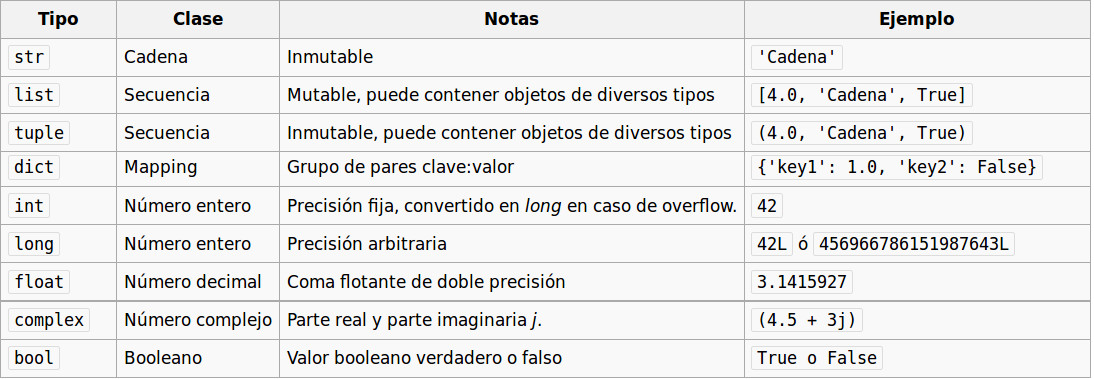
\includegraphics[scale=.4]{imagenes/tipo_datos.jpg}

Se clasifican en:
\begin{description}
 \item[Mutable] si su contenido puede cambiarse.
 \item[Inmutable] si su contenido no puede cambiarse.
\end{description}

Se usa el comando \verb~\type~ para averiguar que tipo de dato contiene una variable

 \begin{lstlisting}
>>> x=1
>>> type(x)
<type 'int'>
>>> x='Ecuaciones'
>>> type(x)
<type 'str'>
\end{lstlisting}





\subsection{Listas y tuples}


\begin{itemize}

\item Es una estructura de dato, que contiene, como su nombre lo indica, listas de otros datos en cierto orden. Listas y tuplas son muy similares.

\item Para declarar una lista se usan los corchetes [], en cambio, para declarar una tupla se usan los paréntesis (). En ambos casos los elementos se separan por comas, y en el caso de las tuplas es necesario que tengan como mínimo una coma.

\item    Tanto las listas como las tuplas pueden contener elementos de diferentes tipos. No obstante las listas suelen usarse para elementos del mismo tipo en cantidad variable mientras que las tuplas se reservan para elementos distintos en cantidad fija.
    
\item Para acceder a los elementos de una lista o tupla se utiliza un índice entero (empezando por "0", no por "1"). Se pueden utilizar índices negativos para acceder elementos a partir del final.


\item Las listas se caracterizan por ser mutables, mientras que las tuplas son inmutables.

\end{itemize}






\begin{lstlisting}
>>> lista = ["abc", 42, 3.1415]
>>> lista[0] # Acceder a un elemento por su indice
'abc'
>>> lista[-1] # Acceder a un elemento usando un indice negativo
3.1415
>>> lista.append(True) # Agregar un elemento al final de la lista
>>> lista
['abc', 42, 3.1415, True]
>>> del lista[3] # Borra un elemento de la lista usando un indice
>>> lista[0] = "xyz" # Re-asignar el valor del primer elemento
>>> lista[0:2] # elementos del indice "0" al "2" (sin incluir  ultimo)
['xyz', 42]
>>> lista_anidada = [lista, [True, 42L]] # Es posible anidar listas
>>> lista_anidada
[['xyz', 42, 3.1415], [True, 42L]]
>>> lista_anidada[1][0] # Acceder a un elemento de una lista dentro de otra lista
True
\end{lstlisting}

\begin{lstlisting}
>>> tupla = ("abc", 42, 3.1415)
>>> tupla[0] # Acceder a un elemento por su indice
'abc'
>>> del tupla[0] # No es posible borrar ni agregar
( Excepcion )
>>> tupla[0] = "xyz" # Tampoco es posible re-asignar
( Excepcion )
>>> tupla[0:2] # elementos del indice "0" al "2" sin incluir
('abc', 42)
>>> tupla_anidada = (tupla, (True, 3.1415)) # es posible anidar
>>> 1, 2, 3, "abc" # Esto tambien es una tupla
(1, 2, 3, 'abc')
>>> (1) #  no es una tupla, ya que no posee al menos una coma
1
>>> (1,) # si es una tupla
(1,)
>>> (1, 2) # Con mas de un elemento no es necesaria la coma final
(1, 2)
>>> (1, 2,) # Aunque agregarla no modifica el resultado
(1, 2)
\end{lstlisting}

\subsection{Diccionarios}
\begin{itemize}
\item    Para declarar un diccionario se usan las llaves \verb~\{\}~. Contienen elementos separados por comas, donde cada elemento está formado por un par clave:valor (el símbolo : separa la clave de su valor correspondiente).
 \item   Los diccionarios son mutables, es decir, se puede cambiar el contenido de un valor en tiempo de ejecución.
\item    En cambio, las claves de un diccionario deben ser inmutables. Esto quiere decir, por ejemplo, que no podremos usar ni listas ni diccionarios como claves.
\item    El valor asociado a una clave puede ser de cualquier tipo de dato, incluso un diccionario.

\end{itemize}






\begin{lstlisting}
>>> dicci = {"cadena": "abc", "numero": 42, "lista": [True, 42L]}
>>> dicci["cadena"] # Usando una clave, se accede a su valor
'abc'
>>> dicci["lista"][0]
True
>>> dicci["cadena"] = "xyz" # Re-asignar el valor de una clave
>>> dicci["cadena"]
'xyz'
>>> dicci["decimal"] = 3.1415927 # nuevo elemento clave:valor
>>> dicci["decimal"]
3.1415927
>>> dicci_mixto = {"tupla": (True, 3.1415), "diccionario": dicci}
>>> dicci_mixto["diccionario"]["lista"][1]
42L
>>> dicci = {("abc",): 42} # tupla puede ser clave pues es inmutable
>>> dicci = {["abc"]: 42} # No es posible que una clave sea una lista
( Excepcion )
\end{lstlisting}



\subsection{Listas por comprensión}
Una lista por comprensión es una expresión compacta para definir listas. Al igual que el operador lambda, aparece en lenguajes funcionales. Ejemplos:


\begin{lstlisting}
>>> range(5) #  "range" devuelve una lista, empezando en 0 \
y terminando con el numero indicado menos uno
[0, 1, 2, 3, 4]
>>> [i*i for i in range(5)]
[0, 1, 4, 9, 16]
>>> lista = [(i, i + 2) for i in range(5)]
>>> lista
[(0, 2), (1, 3), (2, 4), (3, 5), (4, 6)]
\end{lstlisting}



\subsection{Funciones}
\begin{itemize}

  \item  Las funciones se definen con la palabra clave \verb~def~, seguida del nombre de la función y sus parámetros. Otra forma de escribir funciones, aunque menos utilizada, es con la palabra clave \verb~lambda~ (que aparece en lenguajes funcionales como Lisp). Generalemente esta forma es apropiada para funciones que es posible definir en una sola línea.

  \item  El valor devuelto en las funciones con \verb~def~ será el dado con la instrucción \verb~return~.
  \end{itemize}


\begin{lstlisting}
>>> def suma(x, y = 2): # el argumento y tiene un valor por defecto
...     return x + y # Retornar la suma
...
>>> suma(4) # La variable "y" no se modifica, siendo su valor: 2
6
>>> suma(4, 10) # La variable "y" si se modifica
14
\end{lstlisting}


\begin{lstlisting}
>>> suma = lambda x, y = 2: x + y
>>> suma(4) # La variable "y" no se modifica
6
>>> suma(4, 10) # La variable "y" si se modifica
14
\end{lstlisting}

\subsection{Condicionales}
 Una sentencia condicional (\verb~if condicion~) ejecuta su bloque de código interno sólo si \verb~condicion~ tiene el valor bolleano \verb~True~.  Condiciones adicionales, si las hay, se introducen usando \verb~elif~ seguida de la condición y su bloque de código. Todas las condiciones se evalúan secuencialmente hasta encontrar la primera que sea verdadera, y su bloque de código asociado es el único que se ejecuta. Opcionalmente, puede haber un bloque final (la palabra clave \verb~else~ seguida de un bloque de código) que se ejecuta sólo cuando todas las condiciones fueron falsas.



\begin{lstlisting}
>>> verdadero = True
>>> if verdadero: # No es necesario poner "verdadero == True"
...     print "Verdadero"
... else:
...     print "Falso"
...
Verdadero
>>> lenguaje = "Python"
>>> if lenguaje == "C": 
...     print "Lenguaje de programacion: C"
... elif lenguaje == "Python": # Se pueden agregar "elif" como se quiera
...     print "Lenguaje de programacion: Python"
... else: 
...     print "Lenguaje de programacion: indefinido"
...
Lenguaje de programacion: Python
>>> if verdadero and lenguaje == "Python": 
...     print "Verdadero y Lenguaje de programacion: Python"
...
Verdadero y Lenguaje de programacion: Python
\end{lstlisting}






\subsection{Bucles}
El bucle \verb~for~ es similar a  otros lenguajes. Recorre un objeto iterable, esto es  una lista o una tupla, y por cada elemento del iterable ejecuta el bloque de código interno. Se define con la palabra clave \verb~for~ seguida de un nombre de variable, seguido de \verb~in,~ seguido del iterable, y finalmente el bloque de código interno. En cada iteración, el elemento siguiente del iterable se asigna al nombre de variable especificado:

\begin{lstlisting}
>>> lista = ["a", "b", "c"]
>>> for i in lista: # Iteramos sobre una lista, que es iterable
...     print i
...
a
b
c
>>> cadena = "abcdef"
>>> for i in cadena: # Iteramos sobre una cadena, que es iterable
...     print i, # una coma al final evita un salto de linea
...
a b c d e f
\end{lstlisting}



%El bucle \verb~while~ evalúa una condición y, si es verdadera, ejecuta el bloque de código interno. Continúa evaluando y ejecutando mientras la condición sea verdadera. Se define con la palabra clave }verb~while~ seguida de la condición, y a continuación el bloque de código interno:
\begin{lstlisting}
>>> numero = 0
>>> while numero < 10:
...     print numero
...     numero += 1,  #un buen programador modificara las variables de control al finalizar el ciclo while
...
0 1 2 3 4 5 6 7 8 9
\end{lstlisting}


% 
%  \bibliographystyle{plain}
%  \bibliography{biblio}
% 
% 
% \end{document}






% \documentclass{article}
%\documentclass[hyperref={colorlinks=true}]{beamer}
%\documentclass[handout,hyperref={colorlinks=true}]{beamer}


%%%%%%%%%%%%%%%%%%%%%%%%%%%%%%Paquetes%%%%%%%%%%%%%%%%%%%%%%%%%%%%%%%%%%%%%%%%%%%%%%%5
%%%%%%%%%%%%%%%%%%%%%%%%%%%%%%%%%%%%%%%%%%%%%%%%%%%%%%%%%%%%%%%%%%%%%%%%%%%%%%%%%%%%%
\usepackage{empheq}
\usepackage[spanish]{babel}
\usepackage[utf8x]{inputenc}
\usepackage{times}
%\usepackage[T1]{fontenc}
\usepackage{amssymb,amsmath}
\usepackage{enumerate}
\usepackage{verbatim}
\usepackage{ esint }
%\usepackage{pst-all}
%\usepackage{pstricks-add}
\usepackage{array}
%\usepackage[T1]{fontenc}
\usepackage{animate}
%\usepackage{media9}
\usepackage{xparse}
\usepackage{listings}
\usepackage{ wasysym }
\usepackage{sagetex}
\usepackage{yfonts,mathrsfs,eufrak}
\usepackage{hyperref}
\usepackage{color}
\usepackage{url}
\usepackage{theorem}
\usepackage{boiboites}


\definecolor{mygreen}{rgb}{0,0.6,0}
\definecolor{mygray}{rgb}{0.5,0.5,0.5}
\definecolor{mymauve}{rgb}{0.58,0,0.82}

\lstset{ %
  backgroundcolor=\color{white},   % choose the background color; you must add \usepackage{color} or \usepackage{xcolor}
  basicstyle=\footnotesize,        % the size of the fonts that are used for the code
  breakatwhitespace=false,         % sets if automatic breaks should only happen at whitespace
  breaklines=true,                 % sets automatic line breaking
  captionpos=b,                    % sets the caption-position to bottom
  commentstyle=\color{mygreen},    % comment style
  deletekeywords={...},            % if you want to delete keywords from the given language
  escapeinside={\%*}{*)},          % if you want to add LaTeX within your code
  extendedchars=true,              % lets you use non-ASCII characters; for 8-bits encodings only, does not work with UTF-8
  frame=single,	                   % adds a frame around the code
  keepspaces=true,                 % keeps spaces in text, useful for keeping indentation of code (possibly needs columns=flexible)
  keywordstyle=\color{blue},       % keyword style
  language=Python,                 % the language of the code
  otherkeywords={*,...},           % if you want to add more keywords to the set
  numbers=left,                    % where to put the line-numbers; possible values are (none, left, right)
  numbersep=5pt,                   % how far the line-numbers are from the code
  numberstyle=\tiny\color{mygray}, % the style that is used for the line-numbers
  rulecolor=\color{black},         % if not set, the frame-color may be changed on line-breaks within not-black text (e.g. comments (green here))
  showspaces=false,                % show spaces everywhere adding particular underscores; it overrides 'showstringspaces'
  showstringspaces=false,          % underline spaces within strings only
  showtabs=false,                  % show tabs within strings adding particular underscores
  stepnumber=2,                    % the step between two line-numbers. If it's 1, each line will be numbered
  stringstyle=\color{mymauve},     % string literal style
  tabsize=2,	                   % sets default tabsize to 2 spaces
  title=\lstname                   % show the filename of files included with \lstinputlisting; also try caption instead of title
}


%%%%%%%%%%%%%%%%%%%%%%%%%%Nuevos comandos entornos%%%%%%%%%%%%%%%%%%%%%%%%%%%%%%%%
%%%%%%%%%%%%%%%%%%%%%%%%%%%%%%%%%%%%%%%%%%%%%%%%%%%%%%%%%%%%%%%%%%%%%%%%
\newenvironment{demo}{\noindent\emph{Dem.}}{$\square$ \newline\vspace{5pt}}

\newcommand{\com}{\mathbb{C}}
\newcommand{\dis}{\mathbb{D}}
\newcommand{\rr}{\mathbb{R}}
\newcommand{\oo}{\mathcal{O}}
\renewcommand{\emph}[1]{\textcolor[rgb]{1,0,0}{#1}}
\newcommand{\der}[2]{\frac{\partial #1}{\partial #2}}
\renewcommand{\v}[1]{\overrightarrow{#1}}
\renewcommand{\epsilon}{\varepsilon}
%\newcommand{\defverbatim}{\def{#1}}
\renewenvironment{frame}[1]{}{}
\newcommand{\qed}{$\square$}
\DeclareMathOperator{\atan2}{atan2}
\DeclareMathOperator{\sen}{sen}


%%%%%%%%%%%%%%%%%%%%%%%%Colores
\definecolor{myblue}{rgb}{.8, .8, 1}
\definecolor{dblackcolor}{rgb}{0.0,0.0,0.0}
\definecolor{dbluecolor}{rgb}{0.01,0.02,0.7}
\definecolor{dgreencolor}{rgb}{0.2,0.4,0.0}
\definecolor{dgraycolor}{rgb}{0.30,0.3,0.30}
\newcommand{\dblue}{\color{dbluecolor}\bf}
\newcommand{\dred}{\color{dredcolor}\bf}
\newcommand{\dblack}{\color{dblackcolor}\bf}


%%%%%%%%%%Definimos una caja con color
\newlength\mytemplen
\newsavebox\mytempbox
\makeatletter
\newcommand\mybluebox{%
\@ifnextchar[%]
{\@mybluebox}%
{\@mybluebox[0pt]}}
\def\@mybluebox[#1]{%
\@ifnextchar[%]
{\@@mybluebox[#1]}%
{\@@mybluebox[#1][0pt]}}
\def\@@mybluebox[#1][#2]#3{
\sbox\mytempbox{#3}%
\mytemplen\ht\mytempbox
\advance\mytemplen #1\relax
\ht\mytempbox\mytemplen
\mytemplen\dp\mytempbox
\advance\mytemplen #2\relax
\dp\mytempbox\mytemplen
\colorbox{myblue}{\hspace{1em}\usebox{\mytempbox}\hspace{1em}}}
\makeatother
\DeclareDocumentCommand\boxedeq{ m g }{%
{\begin{empheq}[box={\mybluebox[2pt][2pt]}]{equation}% #1%
\IfNoValueF {#2} {\label{#2}}%
#1
\end{empheq}
}%
}


%%%%%%%%%%%%%%%%%%
\newboxedtheorem[boxcolor=orange, background=blue!5, titlebackground=blue!20,
titleboxcolor = black,thcounter=section]{problema}{Problema}{thcounter1}

\newboxedtheorem[boxcolor=orange, background=blue!5, titlebackground=blue!20,
titleboxcolor = black,thcounter=section]{teorema}{Teorema}{thcounter2}

\newboxedtheorem[boxcolor=orange, background=blue!5, titlebackground=blue!20,
titleboxcolor = black,thcounter=section]{definicion}{Definici\'on}{thcounter3}

\newboxedtheorem[boxcolor=orange, background=blue!5, titlebackground=blue!20,
titleboxcolor = black,thcounter=section]{lema}{Lema}{thcounter4}

\newboxedtheorem[boxcolor=orange, background=blue!5, titlebackground=blue!20,
titleboxcolor = black,thcounter=section]{corolario}{Corolario}{thcounter5}

\newboxedtheorem[boxcolor=orange, background=blue!5, titlebackground=blue!20,
titleboxcolor = black,thcounter=section]{proposicion}{Proposici\'on}{thcounter6}

\newboxedtheorem[boxcolor=orange, background=blue!5, titlebackground=blue!20,
titleboxcolor = black,thcounter=section]{codigo}{Función SymPy}{}



        {\theorembodyfont{\normalfont}
\newtheorem{ejemplo}{Ejemplo}}


%%%%%%%%%%%%%%%%%%%%%%%%%%%%%%%%%%%%%%%%%%%%%%%%%%%%%%%%%%%%%%%%%%%%%%%%%%%%%%%%%%%%%%%%%%%%%%%%%%%%%%%%%%%
%%%%%%%%%%Para escibir en clase articulo o similar






\title{Generalidades}
\author{Fernando Mazzone}

%%%%%%%%%%%%%%%%%%%%%%%%%%%%%%%%%%%%%%%%%%%%%%%%%%%%%%%%%%%%%%%%%%%%%%%%%%%%%%%%%%%%%%


\begin{document}
  \maketitle
\tableofcontents


















\section{Sobre esta materia}

\begin{itemize}
 \item  \href{https://docs.google.com/viewer?a=v&pid=sites&srcid=ZGVmYXVsdGRvbWFpbnxlY3VhY2lvbmVzZGlmZXJlbmNpYWxldW5yY3xneDoyZjE0YzJmMDcyODc0ZGQ3}{Programa analítico.}
 \item  \href{https://sites.google.com/site/ecuacionesdiferencialeunrc/ecuaciones-diferenciales-unrc}{Página web} de la materia
 \item  Vamos a hacer uso intensivo de paquetes de matemática basados en \href{https://www.python.org/}{Python}, por ejemplo \href{http://www.scipy.org/}{SciPy},  \href{http://www.scipy.org/}{SymPy} y \href{http://www.sagemath.org/}{SAGE}.
 \item  Requeriremos muchos contenidos de la asignatura Física.
 \item  \begin{tabular}{m{4cm} m{2cm} m{2cm}} Bibliografía principal & 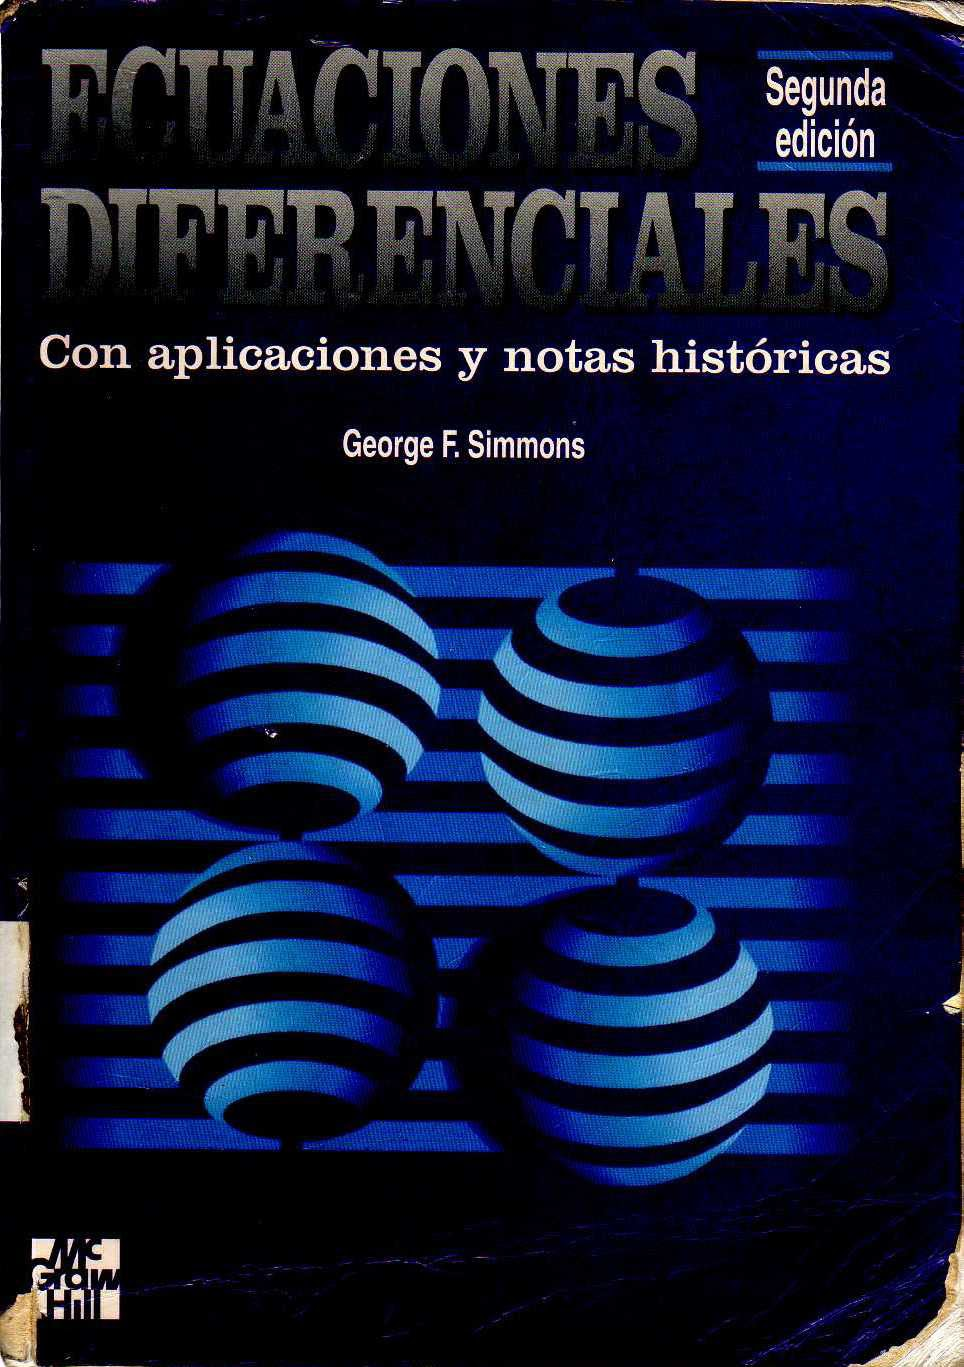
\includegraphics[scale=0.05]{imagenes/Tapa_Simmons.jpg} &    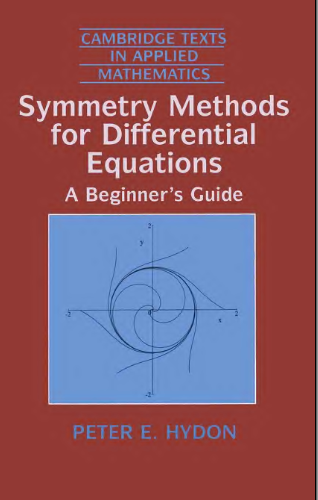
\includegraphics[scale=0.13]{imagenes/tapa_hydon.png}          \end{tabular}

\end{itemize}



\section{¿Que son las ecuaciones diferenciales?}


\begin{definicion}[Ecuación diferencial, definición informal]
 Es una o varias relaciones entre una o varias variables dependientes y sus tasas de cambio respecto a ciertas variables independientes.
 \end{definicion}

 El problema básico asociado
 a las ecuaciones diferenciales es hallar las variables dependientes que las resuelven.

 Las ecuaciones diferenciales son usadas muy a menudo en matemática aplicada, puesto que muchas
 leyes (de la física por ejemplo) se expresan atraves de este tipo de ecuaciones.








 \begin{ejemplo}[\href{http://es.wikipedia.org/wiki/Caída_libre}{Caída libre}] Modelizar matemáticamente el movimiento de un cuerpo de masa $m$ en las proximidades de la superficie
terrestre, asumiendo que su movimiento es
sobre la vertical y que las fuerzas que sobre él actúan son la gravedad y el rozamiento con el aire.
\end{ejemplo}
 \begin{tabular}{m{4.5cm} m{5cm}} 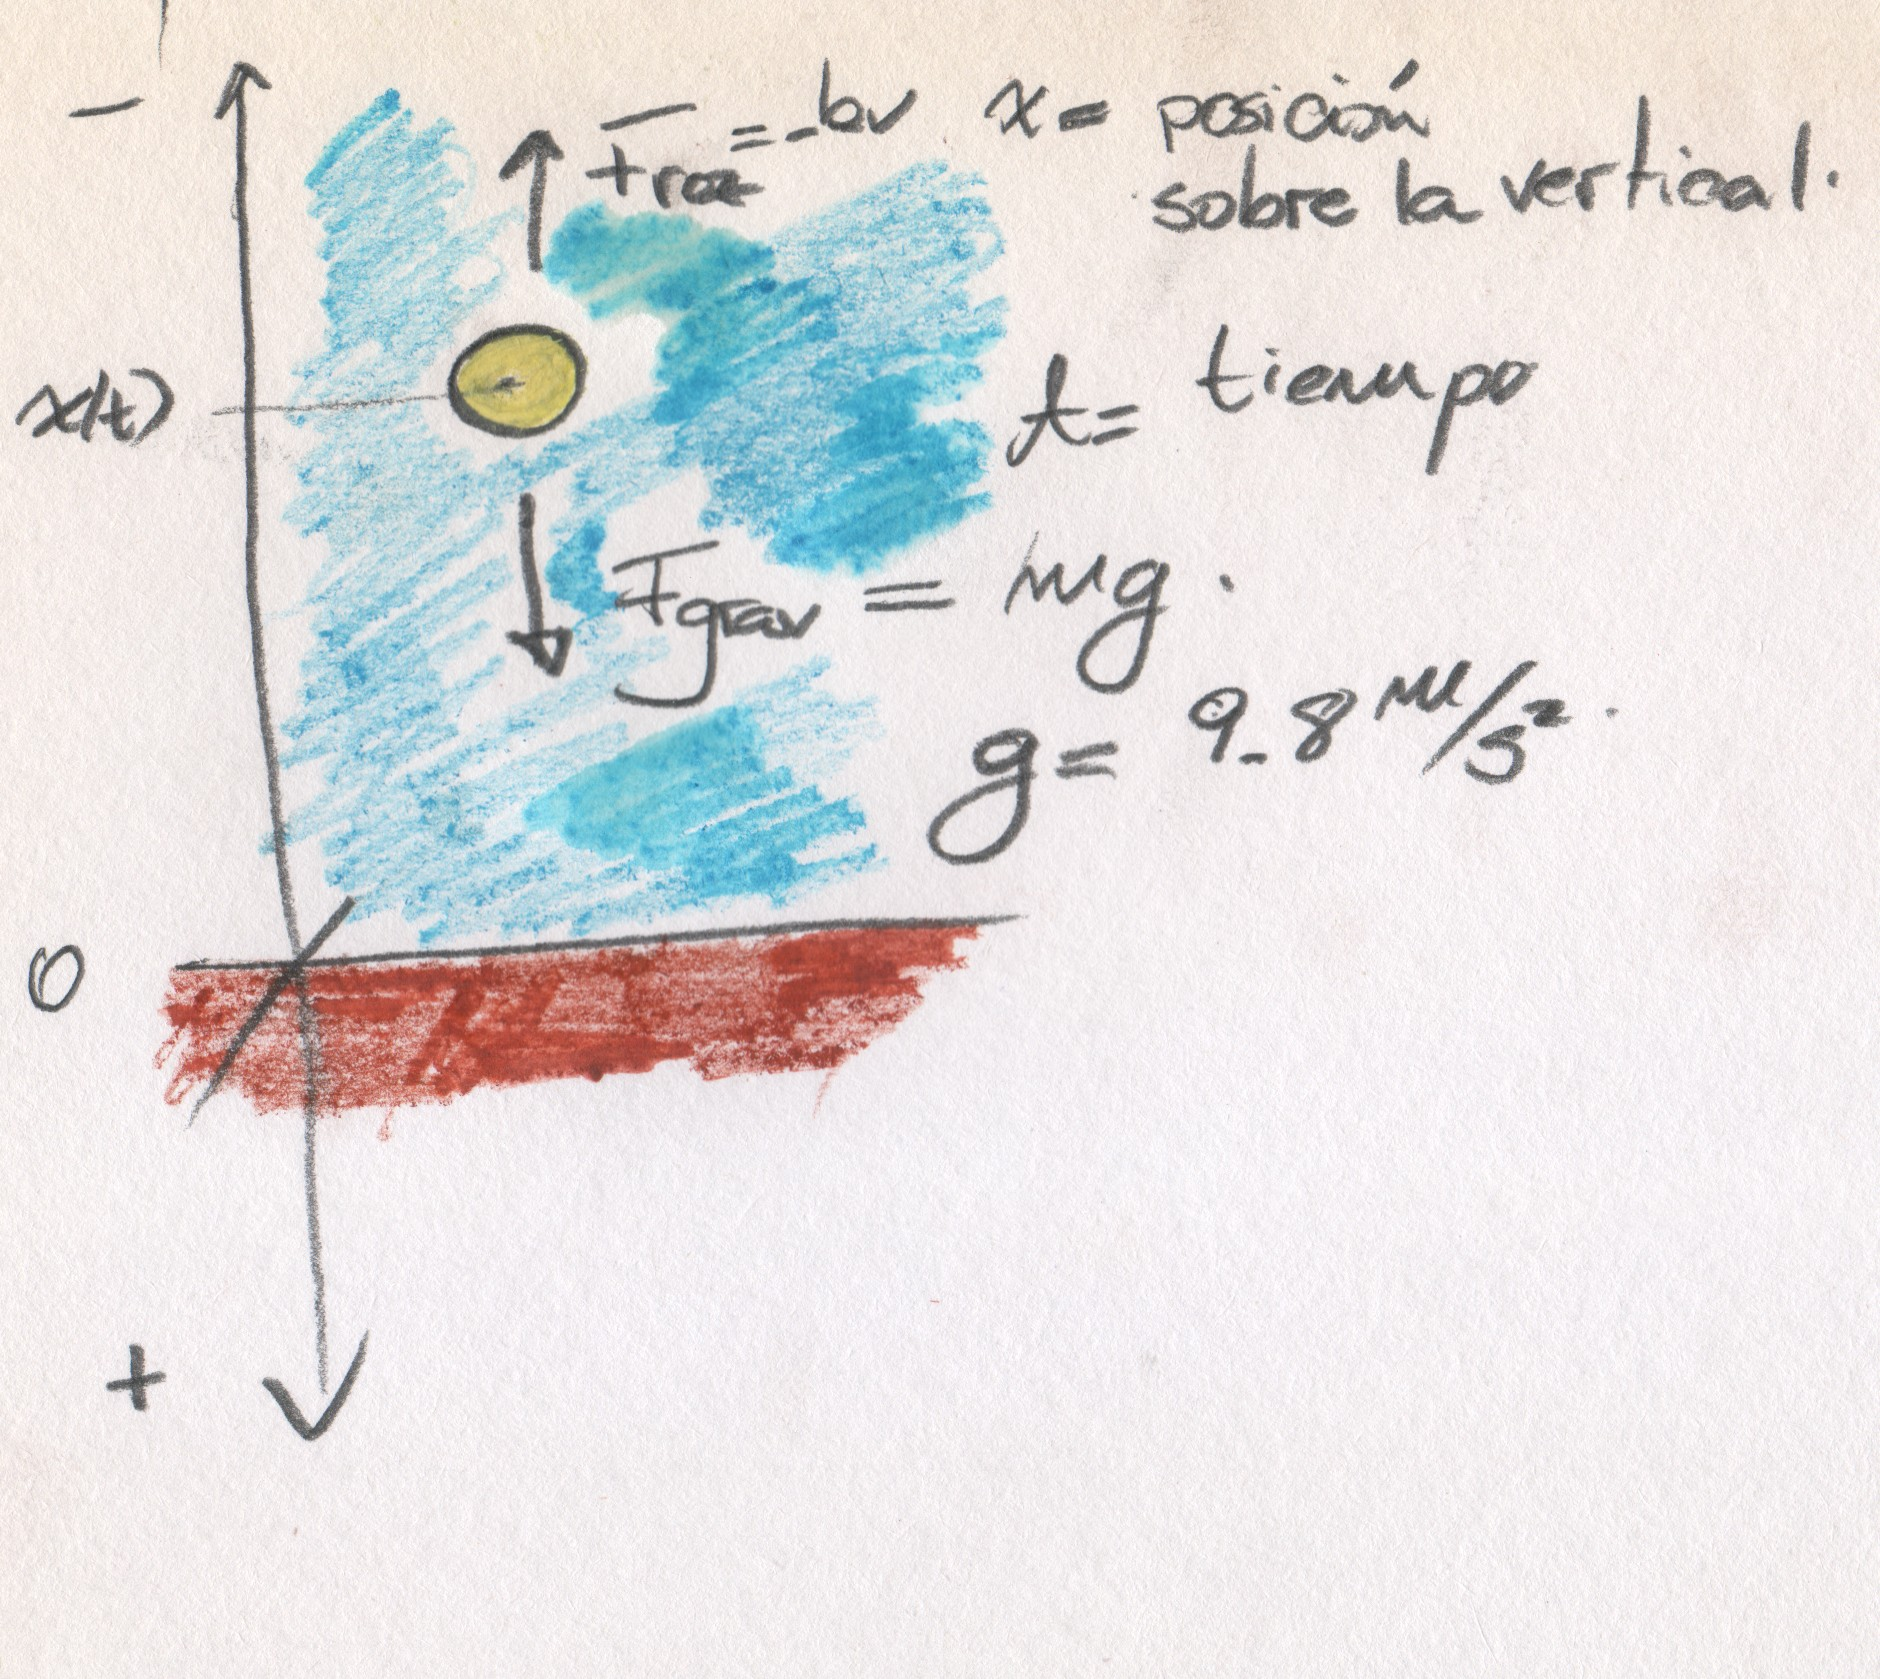
\includegraphics[scale=0.07]{imagenes/caida_libre.jpg}    &  $x(t)=$ posición a lo largo de la vertical, relativo a un eje de coordenadas\newline
$v(t)=\frac{dx}{dt}=$ velocidad\newline
$F_{grav}=$ fuerza debida a la gravedad $=mg$ donde $g=9.8m/s^2$
$F_{roz}=$ fuerza de rozamiento, proporcional a la velocidad y de sentido contrario $=-cv$, $c>0$.

\end{tabular} 



 Usamos la \href{http://es.wikipedia.org/wiki/Leyes_de_Newton}{Segunda Ley de Newton}, esto es la suma de las fuerzas totales que actuan sobre un cuerpo de masa $m$
es igual al producto de la masa $m$ y la aceleración $a(t)$. Recordemos que la aceleración es la tasa de cambio de la velocidad, es decir la derivada segunda de la posición.   

  Usando todas las relaciones mencionadas

\[ma(t)=mv'(t)=F_{\hbox{total}}=F_{\hbox{grav}}+F_{\hbox{roz}}=mg-cv\]

vale decir
\begin{equation}\label{caidaLibre1}
 \boxed{ x''(t)+\frac{c}{m} x'(t)=g.}
\end{equation}
\begin{equation}\label{caidaLibre2}
\boxed{ v'(t)+\frac{c}{m} v=g.}
\end{equation}





\section{Algunos conceptos relacionados con ecuaciones diferenciales}

\begin{definicion}[Orden] El índice de la mayor derivada interviniente en la ecuación.
 \end{definicion}

 Por ejemplo la ecuación \eqref{caidaLibre1} es de orden 2 y la
ecuación \eqref{caidaLibre2}, si bien está estrechamente relacionada con la anterior, es de orden 1. Como regla casi general, cuanto menor es el orden,  más fáciles de estudiar y/o resolver las ecuaciones son.

  \begin{definicion}[Solución] Una función que satisface la relación que indica la ecuación.

   \end{definicion}

   Por ejemplo
\begin{equation}\label{SolGencaidaLibre2} v(t)=\frac{m}{c}g+ke^{-\frac{c}{m}t},\end{equation}
resuelve \eqref{caidaLibre2}, para todo $C\in\rr$. No deberíamos perder tiempo en chequear una cuestión tan sencilla, pero aprovechemos la ocasión para usar  \href{http://www.sympy.org}{SymPy}.





\begin{lstlisting}
>>>from sympy import *
>>>m,g,c,k,t=symbols('m,g,c,k,t')
>>>v=m/c*g+k*exp(-c/m*t)
>>>simplify(v.diff(t)+c/m*v)
g
\end{lstlisting}
Notar que las líneas que comienzan con el signo del prompt \verb~>>>~ indican entradas por línea de comandos y las que comienzan sin este signo son las respuestas del interprete.

Rara vez utilizaremos las siguientes funcionalidades de sympy, pero es oportuno decir que
 \texttt{SymPy} puede encontrar la solución a una ecuación diferencial

\begin{lstlisting}
>>>v=symbols('v',cls=Function)
>>>EqCaida=Eq(v(t).diff(t)+c/m*v(t),g)
>>>Vel=dsolve(EqCaida,v(t))
>>> Vel
v(t) == (g*m + exp(c*(C1 - t/m)))/c
\end{lstlisting}

La solución obtenida es la ya conocida. Es instructivo averiguar que tipo de dato tiene la variable \verb~Vel~

\begin{lstlisting}
>>> type(Vel)
<class 'sympy.core.relational.Equality'>
\end{lstlisting}
A este tipo de cuestiones hay que prestar atención cuando se trabaja con sympy, pues existe la tendencia a confudir los conceptos matemáticos con los propios del lenguaje. Por ejemplo, matemáticamente una solución es una función. Sin embargo, en este caso, cuando le solicitamos una solución a sympy nos entrega un objeto de tipo  ``relación de igualdad``.





\begin{definicion}[Ecuación diferencial ordinaria (EDO)] Es una ecuación donde las variables dependientes sólo dependen de una única variable independiente.
\end{definicion}

Las
ecuaciones \eqref{caidaLibre1} y \eqref{caidaLibre2} son ejemplo de ello, la variable independiente es el tiempo.
  \begin{definicion}[Ecuación en derivadas parciales (EDP)] Es una ecuación donde las variables dependientes dependen de más de una variable independiente.
   \end{definicion}

Ejemplo de este tipo de ecuación es la ecuación de Laplace

\[\frac{\partial^2 u}{\partial x^2}+\frac{\partial^2 u}{\partial y^2}=0\]

Puede ocurrir también que dispongamos de varias ecuaciones diferenciales que se deben satisfacer simultaneamente. En estos casos, el conjuntos de ecuaciones se suele escribir como una única ecuación vectorial. Por este motivo, muchas veces, cuando dispongamos de una única ecuación diremos que tenemos una \emph{ecuación  escalar}.

\begin{definicion}[Sistema de ecuaciones] Es un  conjunto de ecuaciones diferenciales que se deben satisfacer simultaneamente.
 \end{definicion}

En ese caso es  de esperar que tengamos varias incognitas en
nuestro problema. En general una ecuación escalar determina sólo una incognita. De hecho aquí ocurre, a semejanza con ecuaciones algebraicas, que es frecuente necesitar tantas ecuaciones como incognitas.

\begin{ejemplo}[Ecuación del péndulo] El sistema de ecuaciones:
\[\left\{ \begin{array}{l l} x'&=y \\y'&=-\sen(x) \end{array}\right.\]
es muy conocido pues modeliza el movimiento de un péndulo.
\end{ejemplo}



Muy a menudo hablaremos de resolver una ecuación, pero es oportuno discutir que queremos significar con esto.

\begin{definicion}[Resolver una ecuación] Es expresar la solución como combinaciones algebraicas y composiciones de funciones que consideramos elementales.
\end{definicion}

Esta definición contiene una vaga apelación a ciertas ``funciones elementales''. El universo de funciones que se considera elemental es una cuestión política, no matemática. En  principio, consideraremos elementales a las potencias, exponenciales, logarítmos, trigonométricas y trigonométricas inversas. No obstante esta lista se puede expandir con muchas funciones especiales.  Las operaciones permitidas para combinar estas funciones
también están sujetas a convenciones. Por ejemplo, admitiremos como válida una expresión que contenga una integral, al menos en el caso que no sea claro como resolver esta integral.

 Casi todo este curso trata con la discusión de métodos para resolver ecuaciones.  Sin embargo resolver ecuaciones no es quizás el problema principal relacionado con las ecuaciones diferenciales. No importa tanto lograr una expresión formal de la solución, como, por ejemplo, conocer las propiedades que poseen las soluciones. Al fin y al cabo, uno conoce una función a través de sus propiedades.
 





\begin{definicion}[Solución general] Usualmente una ecuación presenta infinitas soluciones. Una solución general  es una expresión que representa todas estas soluciones. Es habitual que una solución general contenga parámetros. Cada elección de estos parámetros determina una solución distinta.
 \end{definicion}

 Por ejemplo \eqref{SolGencaidaLibre2} es la solución general de \eqref{caidaLibre2}.
  La afirmación anterior requiere una demostración puesto que sólo hemos mostrado que \eqref{SolGencaidaLibre2} es solución, pero no
que toda solución se expresa con \eqref{SolGencaidaLibre2}. Para demostrar la afirmación, hay que multiplicar ambos miembros de \eqref{caidaLibre2} 
por $e^{\frac{c}{m}t}$ y luego integrar respecto a $t$ 
\[\frac{mg}{c}e^{\frac{c}{m}t}=\int ge^{\frac{c}{m}t}dt=\int v'(t)e^{\frac{c}{m}t}+\frac{c}{m}e^{\frac{c}{m}t} vdt=e^{\frac{c}{m}t}v+C.\]
 Despejando $v$ del primer y último miembro obtenemos \eqref{SolGencaidaLibre2} con $k=-C$.

 




\begin{ejemplo} En algunas ocasiones sólo podemos dejar una relación implícita entre las variable dependientes e independientes. Por ejemplo
\begin{equation}\label{solImpl}x=e^y+y+C\quad\text{ para } C\in\rr\end{equation}
es solución general de
\[y'(e^y+1)=1.\]
Vamos a chequear sólo que \eqref{solImpl} es solución, dejando la justificación que toda solución tiene esa forma para más adelante. Derivando \eqref{solImpl}
\[ 1=e^yy'+y'\]
Luego $y'=1/(1+e^{y})$. Reemplazando esta relación  en la ecuación diferencial corroboramos que es solución.
\end{ejemplo}



\section{Definición formal}

\begin{definicion}[Ecuación diferencial] Una ecuación diferencial ordinaria de orden $n$ es una relación de la forma
\[\boxed{F(x,y(x),y'(x),\ldots,y^{(n)}(x))=0}.\]
donde $F:(a,b)\times \Omega\to\rr$, $\Omega$ es abierto de $\rr^{n+1}$ y $(a,b)$ un intervalo de $\rr$.
  \end{definicion}





\begin{ejemplo} El problema de hallar una primitiva de una función es una ecuación diferencial que, como ya has visto en cursos iniciales de análisis, se relaciona con el concepto de integral. Supongamos $f:(a,b)\subset \rr\to\rr$ una función continua. Consideremos la ecuación diferencial
\[y'(x)=f(x).\]
Sea $x_0\in(a,b)$, integrando respecto a $x$ entre $x_0$ y $x$
\[y(x)=y(x_0)+\int_{x_0}^xf(t)dt\]
Que es una solución general. Quedaría determinada una única solución si, por ejemplo, conociecemos $y(x_0)$.
\end{ejemplo}



\begin{ejemplo} Supongamos $f:(a,b)\subset \rr\to\rr$ como antes. Consideremos la ecuación diferencial
\[y''(x)=f(x).\]
Tomemos una integral indefinida respecto a $x$ 
\[y'(x)=C_1+\int f(t)dt\]
Ahora deberemos tomar una integral indefinida más
\[y(x)=C_2+C_1t +\int\left(\int f(x)dx\right)dx.\]
Ahora quedan dos constantes $C_1$ y $C_2$. 
\end{ejemplo}



 \begin{definicion}[Principio de Hadamard]
 Un problema se dice \href{http://es.wikipedia.org/wiki/Problema_bien_definido}{bien planteado} segun Hadamard si satisface que
 \begin{enumerate}
  \item El problema admite solución
  \item La solución es única
  \item La solución depende de manera continua de los datos numéricos del problema.
 \end{enumerate}
\end{definicion}

 Como hemos visto, una ecuación diferencial no determina una única solución, por consiguiente no sería un problema bien planteado. Debemos agregar relaciones
a nuestro problema para que sea bien planteado. Es así que aparecen condiciones iniciales, problemas de contorno, etc.
 




\begin{definicion}[Problemas de valores iniciales] Sea $x_0\in(a,b)$, $F:(a,b)\times \Omega\to\rr$ e $y_0,y_0^1,\ldots,y_0^{n-1}\in\rr$. Las siguientes relaciones  se denominan problema de
valores iniciales
\[
 \left\{\begin{array}{l l l}
         F(x,y,y',&\ldots,y^{(n)})=0& x\in(a,b)\\
         y(x_0)&=y_0&\\
         y'(x_0)&=y_0^1&\\
          & \vdots &\\
          y^{(n-1)}(x_0)&=y_0^{n-1}&\\
        \end{array}
   \right.
\]

\end{definicion}



\begin{definicion}[Ecuaciones de primer orden] La ecuación general de primer orden tiene la forma
\[
F(x,y(x),y'(x))=0,
\]
donde $F:(a,b)\times \Omega\to\rr$ y $\Omega$ abierto de $\rr^2$. Con frecuencia asumiremos que $y'$ se despeja de la relación anterior, es decir que existe $f:\Omega'\to\rr$,
$\Omega'$ abierto de $\rr^2$, tal que
\[y'=f(x,y).\]
Bajo esta suposición, si $(x_0,y_0)\in\Omega'$ el problema de valores iniciales se escribe
\[\left\{\begin{array}{l l}
	    y'&=f(x,y)\\
	    y(x_0)&=y_0
         \end{array}\right.
\]
\end{definicion}



\section{Familias paramétricas de funciones}

En las secciones siguientes vamos a describir problemas, matemáticos y físicos que se reducen a un problema de ecuaciones diferenciales.


\begin{problema}
Dada una familia paramétrica de funciones
 \begin{equation}\label{flia_param}y=y(x,c),\end{equation}
 dependiente del parámetro $c\in\rr$, ¿Será posible hallar una ecuación para la cual la familia sea la solución general?
\end{problema}


{Familias paramétricas de funciones}
En líneas generales la respuesta es si. Nos conviene expresar \eqref{flia_param} como una ecuación implícita
\begin{equation}\label{flia_impl}f(x,y,c)=0.\end{equation}
Derivando esta ecuación respecto a $x$
\begin{equation}\label{der_impl}
 \frac{\partial f}{\partial x}+\frac{\partial f}{\partial y}y'(x,c)=0.
\end{equation}
Ahora es posible eliminar $c$ de \eqref{flia_impl} y \eqref{der_impl} al costo de quedarnos con una sola ecuación.




\begin{ejemplo} Encontrar la ecuación que satisface la familia paramétrica
\[x^2+y^2=c^2.\]
Derivamos
\[2x+2yy'=0.\]
Ya está!!!
\end{ejemplo}

\begin{ejemplo} Idem $x^2+y^2=2cx$.  Derivando
\[2x+2yy'=2c.\]
Eliminamos $c$ de las dos relaciones
\[\frac{x^2+y^2}{x}=2x+2yy'\Rightarrow \boxed{y'=\frac{y^2-x^2}{2xy}}.\]
\end{ejemplo}


\begin{problema}
 Dada una familia paramétrica
 \[f(x,y,c)=0,\]
 encontrar otra
 \[g(x,y,d)=0\]
 tal que los ángulos que forman los gráficos entre las funciones de una y de otra familia sean rectos  en cada punto de corte entre ellos.
\end{problema}




Para resolver este problema se completan estos pasos
\begin{itemize}
 \item Se encuentra la ecuación diferencial que satisface la familia dada, digamos
 \[y'=h(x,y).\]
 \item Se resuelve
 \[y'=-\frac{1}{h(x,y)}.\]
\end{itemize}




\begin{ejemplo} Encontrar la familia de curvas ortogonales a la flia de circunferencias

\[x^2+y^2=c^2\]

Hallamos antes que la ecuación que satisfacen estas curvas es
\[y'=-\frac{x}{y}.\]
Luego deberíamos resolver
\[y'=\frac{y}{x}.\]
Que no sabemos pero SymPy si!!!

\end{ejemplo}

\begin{codigo}[\texttt{dsolve}]

\textbf{Sintaxis} (\href{http://docs.sympy.org/latest/modules/solvers/ode.html#}{documentación \texttt{SymPy}})

\texttt{dsolve(eq, f(x), hint)}

\texttt{eq:} Ecuación (posicional)

\texttt{f(x):} función incognita (posicional)

\texttt{hint: } Método a emplear. Argumento con nombre \texttt{hint='cadena'}.

\end{codigo}

\begin{ejemplo}
\end{ejemplo}
\begin{lstlisting}
x=symbols('x')
y=Function('y')(x)
MiEcua=Eq(y.diff(x),y/x)
f=dsolve(MiEcua,y)
\end{lstlisting}

\noindent\textbf{Resultado:}
Flía rectas  por el origen. \\
La instrucción\\
\texttt{f=dsolve(MiEcua,y,hint='separable')}
\\produce el mismo resultado.






\begin{codigo}[\texttt{plot}]

\textbf{Sintaxis} (\href{http://docs.sympy.org/latest/modules/plotting.html}{documentación \texttt{SymPy}})

Para un gráfico simple

\texttt{plot(expr,rango,opcionales(claves))}

\texttt{expr:} Expresión a graficar 

\texttt{rango:} Conjunto donde varia la variable independiente 

\texttt{opcionales } Argumentos que modifican la apariencia del gráfico. Generalemente de la forma de clave=valor

\end{codigo}


\begin{ejemplo}

\end{ejemplo}


\begin{lstlisting}
x=symbols('x')
f=plot(1/x,(x,-3,3),ylim=(-3,3))
\end{lstlisting}

\noindent\textbf{Resultado:}
\begin{center}
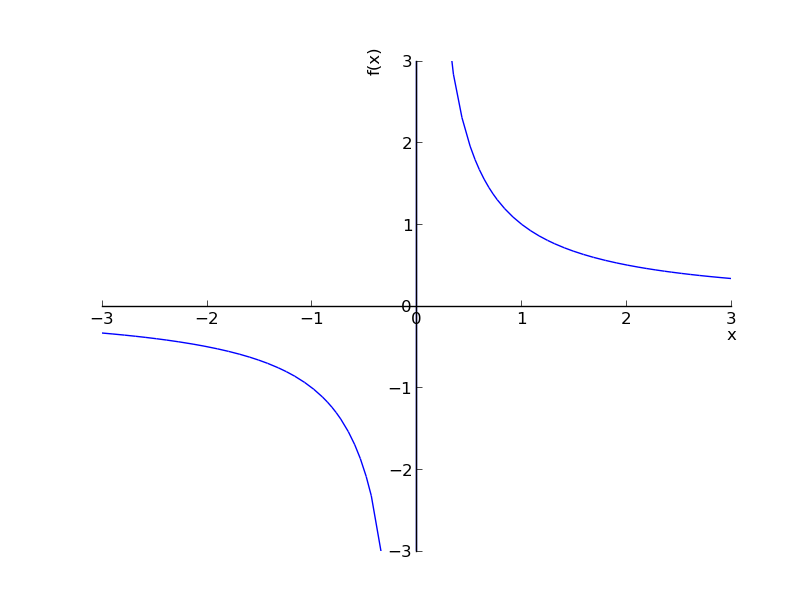
\includegraphics[scale=.35]{imagenes/ejemplo_plot.png}
\end{center}












\begin{ejemplo}Grafiquemos un familias paramétrica de funciones.

\end{ejemplo}




\begin{lstlisting}
from sympy import *
x,y=symbols('x,y')
Rango=range(21)
L=[tan(pi*k/21.0) for k in Rango] 
p=plot(L[0]*x,(x,-2,2),show=False,xlim=(-2,2),\
ylim=(-2,2),aspect_ratio=(1,1))
for pend in L[1:]:
    p1=plot(pend*x,(x,-2,2),show=False,\
xlim=(-2,2),ylim=(-2,2),aspect_ratio=(1,1))
    p.append(p1[0])
for r in range(1,10):
    p1=plot_implicit(Eq(x**2 + y**2, 0.2*r),\
show=False,aspect_ratio=(1,1),xlim=(-2,2),ylim=(-2,2))
    p.append(p1[0])
\end{lstlisting}


\noindent\textbf{Resultado:}
\begin{figure}[h]
\begin{center}
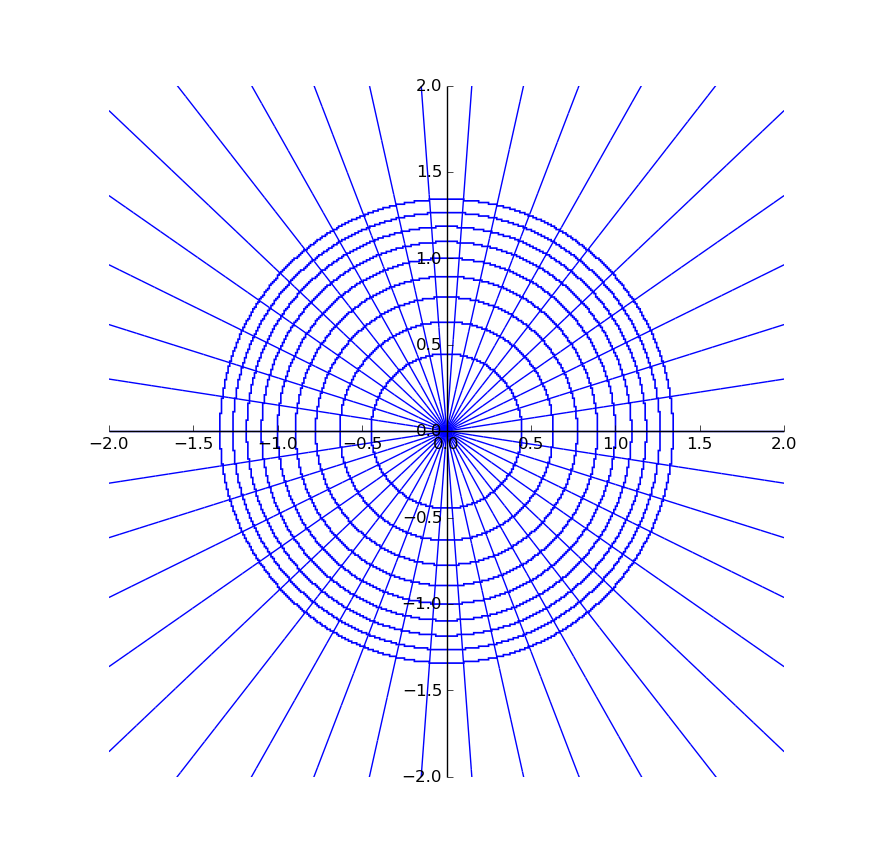
\includegraphics[scale=.2]{imagenes/flia_curvas_ortogonales.png}
\end{center}
\caption{Familia curvas ortogonales}\label{fig:ortogonales}
\end{figure}


\begin{problema}[Familias paramétricas de funciones en coordenadas polares]
En ocasiones la ecuación de la familia de curvas esta dada en otras coordenadas. Por ejemplo supongamos que tenemos la flia de curvas dadas por una EDO en coordenadas polares
\[\frac{dr}{d\theta}=f(r,\theta)\label{eq:flia_curvas_polar},\]
y queremos hallar su flia ortogonal.
\end{problema}

\noindent\textbf{Solución:} Calculemos $dy/dx$ para las curvas en la familia dada.
\[\frac{dy}{dx}=\frac{dy/d\theta}{dx/d\theta}=\frac{r_{\theta}\sen\theta+r\cos\theta}{r_{\theta}\cos\theta-r\sen\theta}=\frac{f\sen\theta+r\cos\theta}{f\cos\theta-r\sen\theta},\]

donde $r_{\theta}=dr/d\theta$. La flia ortogonal tiene que satisfacer

\[\frac{dy}{dx}=-\frac{f\cos\theta-r\sen\theta}{f\sen\theta+r\cos\theta}\]
Luego
\[\frac{r_{\theta}\sen\theta+r\cos\theta}{r_{\theta}\cos\theta-r\sen\theta}=-\frac{f\cos\theta-r\sen\theta}{f\sen\theta+r\cos\theta}.\]
Si despejamos $r_{\theta}$ llegamos a la ecuación de la flia de curvas ortogonales en coordenadas polares

\boxedeq{\frac{dr}{d\theta}=-\frac{r^2}{f}.}{eq_flia_ortogonal_polares}




\section{Separación de variables}

\begin{definicion}[Ecuaciones en variables separadas] Se dice que en una ecuación de primer orden
 \[y'=f(x,y)\]
 separan las variables, si es posible la factorización $f(x,y)=g(x)h(y)$.
\end{definicion}



Una ecuación  en la que se separan variables se puede resolver siguiendo los siguientes pasos. Como, asumiendo $h(y)\neq 0$,
\[\frac{y'}{h(y)}=g(x),\]
Si $H$ y $G$ son primitivas de $1/h$ y $g$ respectivamente por la regla de la cadena tenemos
\[\frac{d}{dx}H(y)=\frac{d}{dx}G(x)\]
Luego 
\[H(y)=G(x)+C,\quad C\in\rr.\]
Por último, si podemos encontrar la inversa de $H$
\boxedeq{y(x)=H^{-1}\left(G(x)+C\right).}{eq:var_sep}
será candidata a solución general. No podemos estar seguros de esta afrirmación, sobre todo porque la deducción de esta fórmula estuvo sujeta a suposiciones, como $h(y)\neq 0$.



\begin{ejemplo} Resolver
\[y'=\frac{y}{x}.\]
Es común emplear el método de la siguiente forma
\[\begin{split}
   \frac{dy}{dx}=\frac{y}{x} &\Longrightarrow \frac{dy}{y}=\frac{dx}{x} \Longrightarrow \int \frac{dy}{y}=\int \frac{dx}{x}\\
   &\Longrightarrow\ln|y|=\ln|x|+C \Longrightarrow |y|= k|x|, \hbox{ con }k>0\\
   &\Longrightarrow y= kx, \hbox{ con }k\in\rr
  \end{split}
\]
\end{ejemplo}




\begin{codigo}{\texttt{classify\_ode}: clasificación de ecuaciones}

\textbf{Sintaxis}\\
\texttt{classify\_ode(eq, f(x))}\\

\end{codigo}
\begin{ejemplo}

\end{ejemplo}

\begin{lstlisting}
x=symbols('x')
y=Function('y')(x)
MiEcua=Eq(y.diff(x),y/x)
tipo=classify_ode(MiEcua,y)
\end{lstlisting}
\textbf{Resultado:}\\
\begin{verbatim}
('separable', '1st_exact', '1st_linear', 
'almost_linear', 'lie_group',  etc)
\end{verbatim}




\section{Galeria de Ejemplos}

Vamos a describir algunos ejemplos. algunos de ellos llevan a problemas matemáticos muy simples. No obstante es oportuno discutirlos por dos motivos, habituarnos a la utilización de la matemática para resolver problemas de otras ciencias y sentar las bases para discutior problemas más relevantes desde una óptica matemática.

\subsection{Ley de reproducción normal}
  En muchos ejemplos de biología, química-física, etc, hay magnitudes que crecen(decrecen) siguiendo una ley que denominaremos
\href{http://es.wikipedia.org/wiki/Crecimiento_exponencial}{Ley de reproducción  normal}. Según esta ley la cantidad de individuos, sustancia, materia,
energía, etc, que se agrega o elimina de una población, cuerpo, etc por unidad de tiempo es proporcional a la cantidad de individuos, sustancia, etc que hay presente.   Una población de seres vivos puede reproducirse de esta manera bajo algunas circunstancias
especiales, por ejemplo si cuenta con fuente ilimitada de alimentos.

  Si $P(t)$ es la cantidad de individuos en el momento $t$, la ley de reproducción normal establece
en este caso la siguiente ecuación diferencial de primer orden
\[P'(t)=kP(t),\quad\text{ con } k>0.\]
La solución es hallada con suma facilidad, siendo ella 
\[\boxed{P(t)=Ce^{kt},\quad C\in\rr.}\]
La constante  $C$ se puede determinar si tenemos un problema a valores iniciales (pvi), por ejemplo $P(0)=P_0$, siendo $P_0\in\rr$ dado. En ese caso
$A=P_0$. 



  Otro ejemplo de comportamiento similar es la \href{http://es.wikipedia.org/wiki/Radiactividad}{desintegración radiactiva}. Algunos átomos de
ciertas sustancias, pueden ``desarmarse'' en átomos de otras sustancias. En el proceso suelen emitir radiaciones.  La velocidad de desintegración sigue una ley
de reproducción normal pero hay que tener en cuenta que la materia radiactiva, es decir la ``población''  en este caso, se pierde. Si $x(t)$ es la masa de materia radiactiva en el momento $t$, evolucionará
acorde a la ley
\[\boxed{x'(t)=-kx(t),\quad\text{con } k>0.}\]



\subsection{Soluciones}

\begin{problema}
\begin{tabular}{m{5cm} m{4.5cm}}
 Un tanque contiene inicialmente $N$ $\hbox{m}^3$ de $H_2O$ entre los cuales hay disueltos $C$ kg de sal común
 $NaCl$. A través de una boca de entrada y una de salida empieza circular la solución, entrando y saliendo al mismo caudal $q\frac{\hbox{m}^3}{s}$. Se supone que 
 la solución entrante tiene una concentración conocida $r$. Encontrar la cantidad de sal en el momento $t$. &
  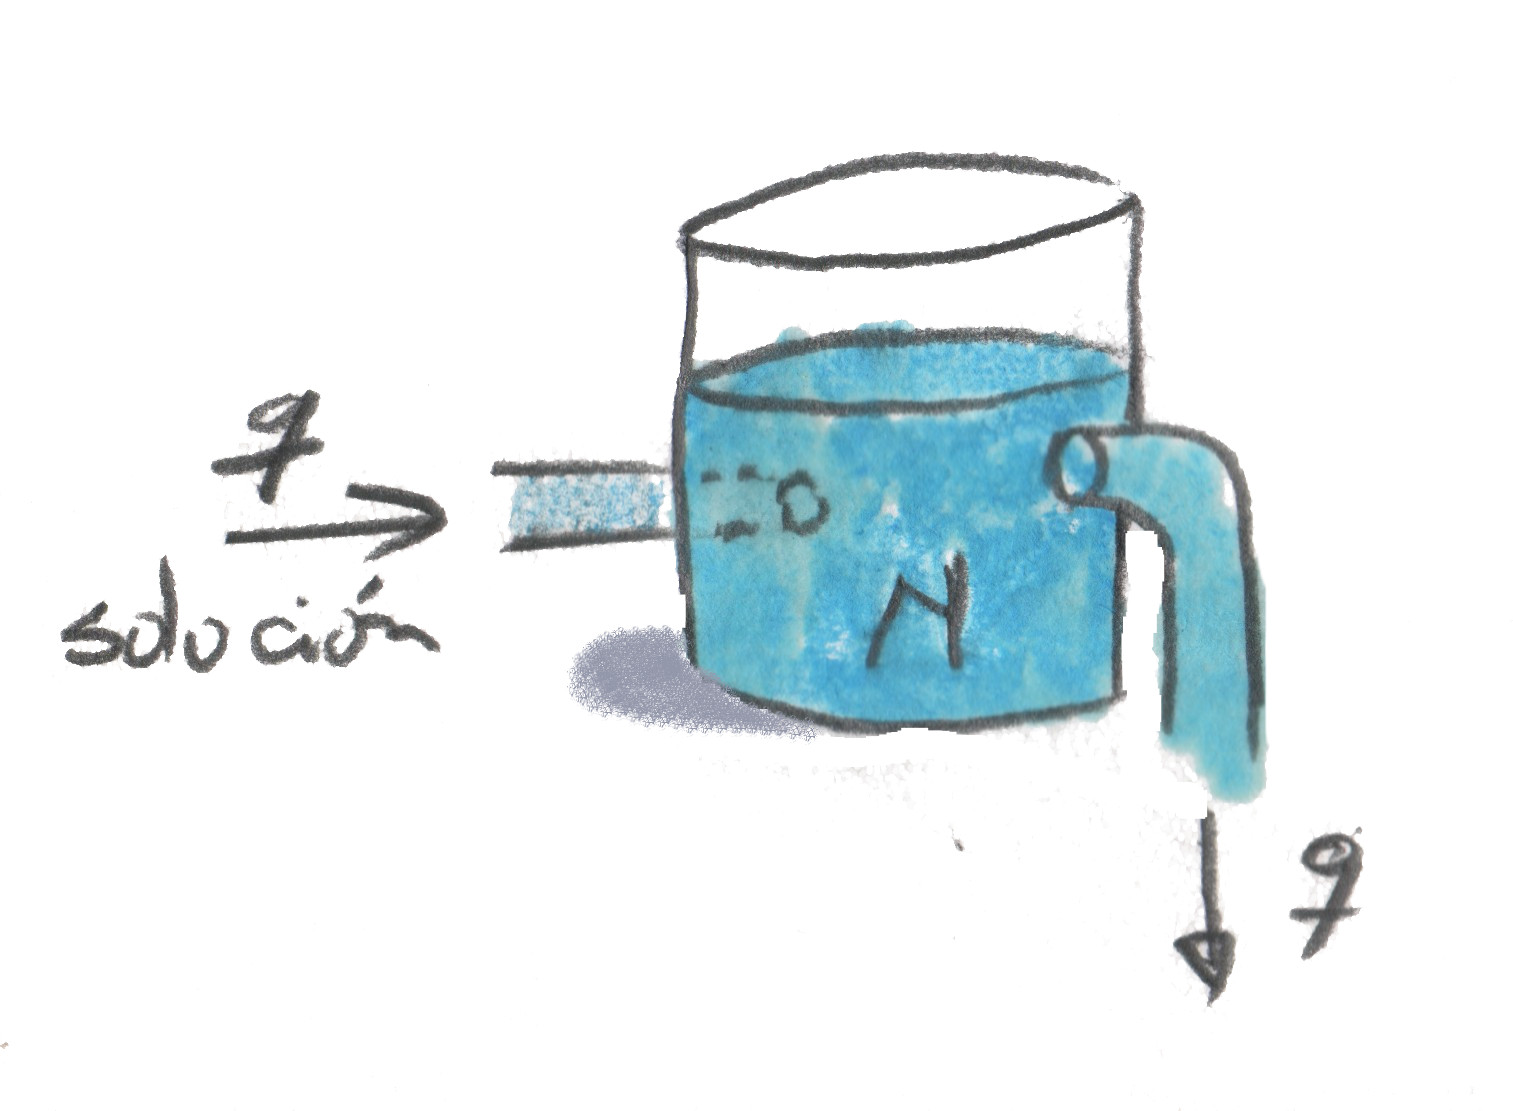
\includegraphics[scale=.1]{imagenes/tanque.jpg} \\
\end{tabular}
\end{problema}


 Sea $x(t)$ la cantidad de $NaCl$ en el tanque en el momento $t$. entonces

\[\begin{split}
   x'(t)&=\text{cantidad que entra }-\text{cantidad que sale }\\
          &=qr-q\frac{x(t)}{N}
  \end{split}
\]




\subsection{Dinámica del punto}

\subsubsection{Discusión Teórica}
Vamos a recordar algunas temas de la asignatura física. En particular  el movimiento de un cuerpo de masa $m$ al que podemos suponer puntual. Lo llamaremos punto masa. Denotamos por $x(t)$ su posición, digamos en $\rr^3$. Suponemos
que sobre él actúa una fuerza $f$. Recordemos que $x'(t)$ es la velocidad $v(t)$ y que $x''(t)$ es la aceleración $a(t)$.  
\href{http://es.wikipedia.org/wiki/Leyes_de_Newton\#Segunda_ley_de_Newton_o_ley_de_fuerza}{La segunda ley de Newton} implica que 
\begin{equation}\label{2leyR}\boxed{mx''(t)=f}\end{equation}


Supongamos que el movimiento del punto masa se realiza entre los momentos $t_0$ y $t_1$. Como has visto en Cálculo III la lóngitud de la curva recorrida 
$s(t)$ se puede calcular por
\begin{equation}\label{2ley}s=\int_{t_0}^{t_1}|x'(t)|dt=\int_{t_0}^{t_1}|v(t)|dt.\end{equation}
A $s$ se lo suele denominar \href{http://es.wikipedia.org/wiki/Longitud_de_arco}{elemento de arco}. Es comun querer utilizar a $s$ como variable independiente en 
lugar de $t$, puesto que algunas fórmulas se simplifican de esta forma. Por ejemplo

\begin{equation}\label{pre_trab} f\cdot v(t)dt=f\cdot\frac{v(t)}{|v(t)|}|v(t)|dt=f_tds,\end{equation}
donde $f_t$ denota la proyección de la fuerza $f$ sobre la dirección tangente a la trayectoria.





Si integramos \eqref{pre_trab} entre $t_0$ y $t_1$ y usamos \eqref{2leyR} obtenemos
\[\begin{split} W:=\int_{s_0}^{s_1}f_t(x(s))ds&=\int_{t_0}^{t_1} f(x(t))\cdot v(t)dt\\
   & =m \int_{t_0}^{t_1} v'(t)\cdot v(t)dt\\
   &=\frac{m}{2} \int_{t_0}^{t_1} \frac{d|v|^2}{dt}dt\\
   &=\frac{m}{2}|v(t_1)|^2-\frac{m}{2}|v(t_0)|^2.  \end{split}\]


  A la cantidad $\frac{m}{2}|v|^2$ se la denomina \emph{energía cinética} $E_c$ y a $W$ se lo denomina \emph{trabajo}.
Las relaciones obtenidas dicen que la variación de la energía cinética es igual al trabajo realizado $W=\Delta E_c$ por la fuerza $f$.
El trabajo realizado depende de la proyección tangencial de la fuerza $f_t$.  Llamaremos a esta relación
\href{https://es.wikipedia.org/wiki/Conservaci%C3%B3n_de_la_energ%C3%ADa}{Principio de Conservación de la Energía Mecánica.}

  Vamos a referirnos por \emph{rapidez} al módulo de la velocidad.
Si uno quiere incrementar o reducir la rapidez final $|v(t_1)|$ entonces deberá tener fuerzas con una componente tangencial no nula. 
Dicho de otra forma, si la fuerza es perpendicilar al movimiento, no hay cambio de rapidéz. 

  Hay fuerzas que siempre actuan en la dirección del movimiento. El ejemplo más conocido son las fuerzas de fricción, resistencia del aire,
resistencia a la rodadura, etc. Estás fuerzas, actúan sólo en la dirección del movimiento y se oponen a él.


 

  Por el contrario hay otras que actúan perpendiculares al movimiento $f_t=0$. Ejemplo de ello son las fuerzas que mantienen a un cuerpo moviéndosé a lo largo
de una guía. Por ejemplo un niño cayendo por un tobogan. Que el niño no se despegue de la guía (tobogán) se explica por la aparición de una fuerza que se denomina
reacción de vínculo que actúa en la dirección perpendicular al movimiento esto es decir a la guía. Está fuerza debe compensar a toda otra fuerza que trata de apartar
al cuerpo de la guía.  En el caso del tobogán la gravedad trata de apartar al niño de aquel.





\subsubsection{Cuerpos cayendo por guías}
Analicemos más en detalle el movimiento de un cuerpo cayendo a lo largo de una guía estando además influído  por la acción de la gravedad. Supondremos el movimiento en las proximidades de la superficie de la Tierra y por ello, supondremos que la fuerza de la gravedad es la constante $mg$. 

\begin{tabular}{m{5cm} m{4.5cm}}
 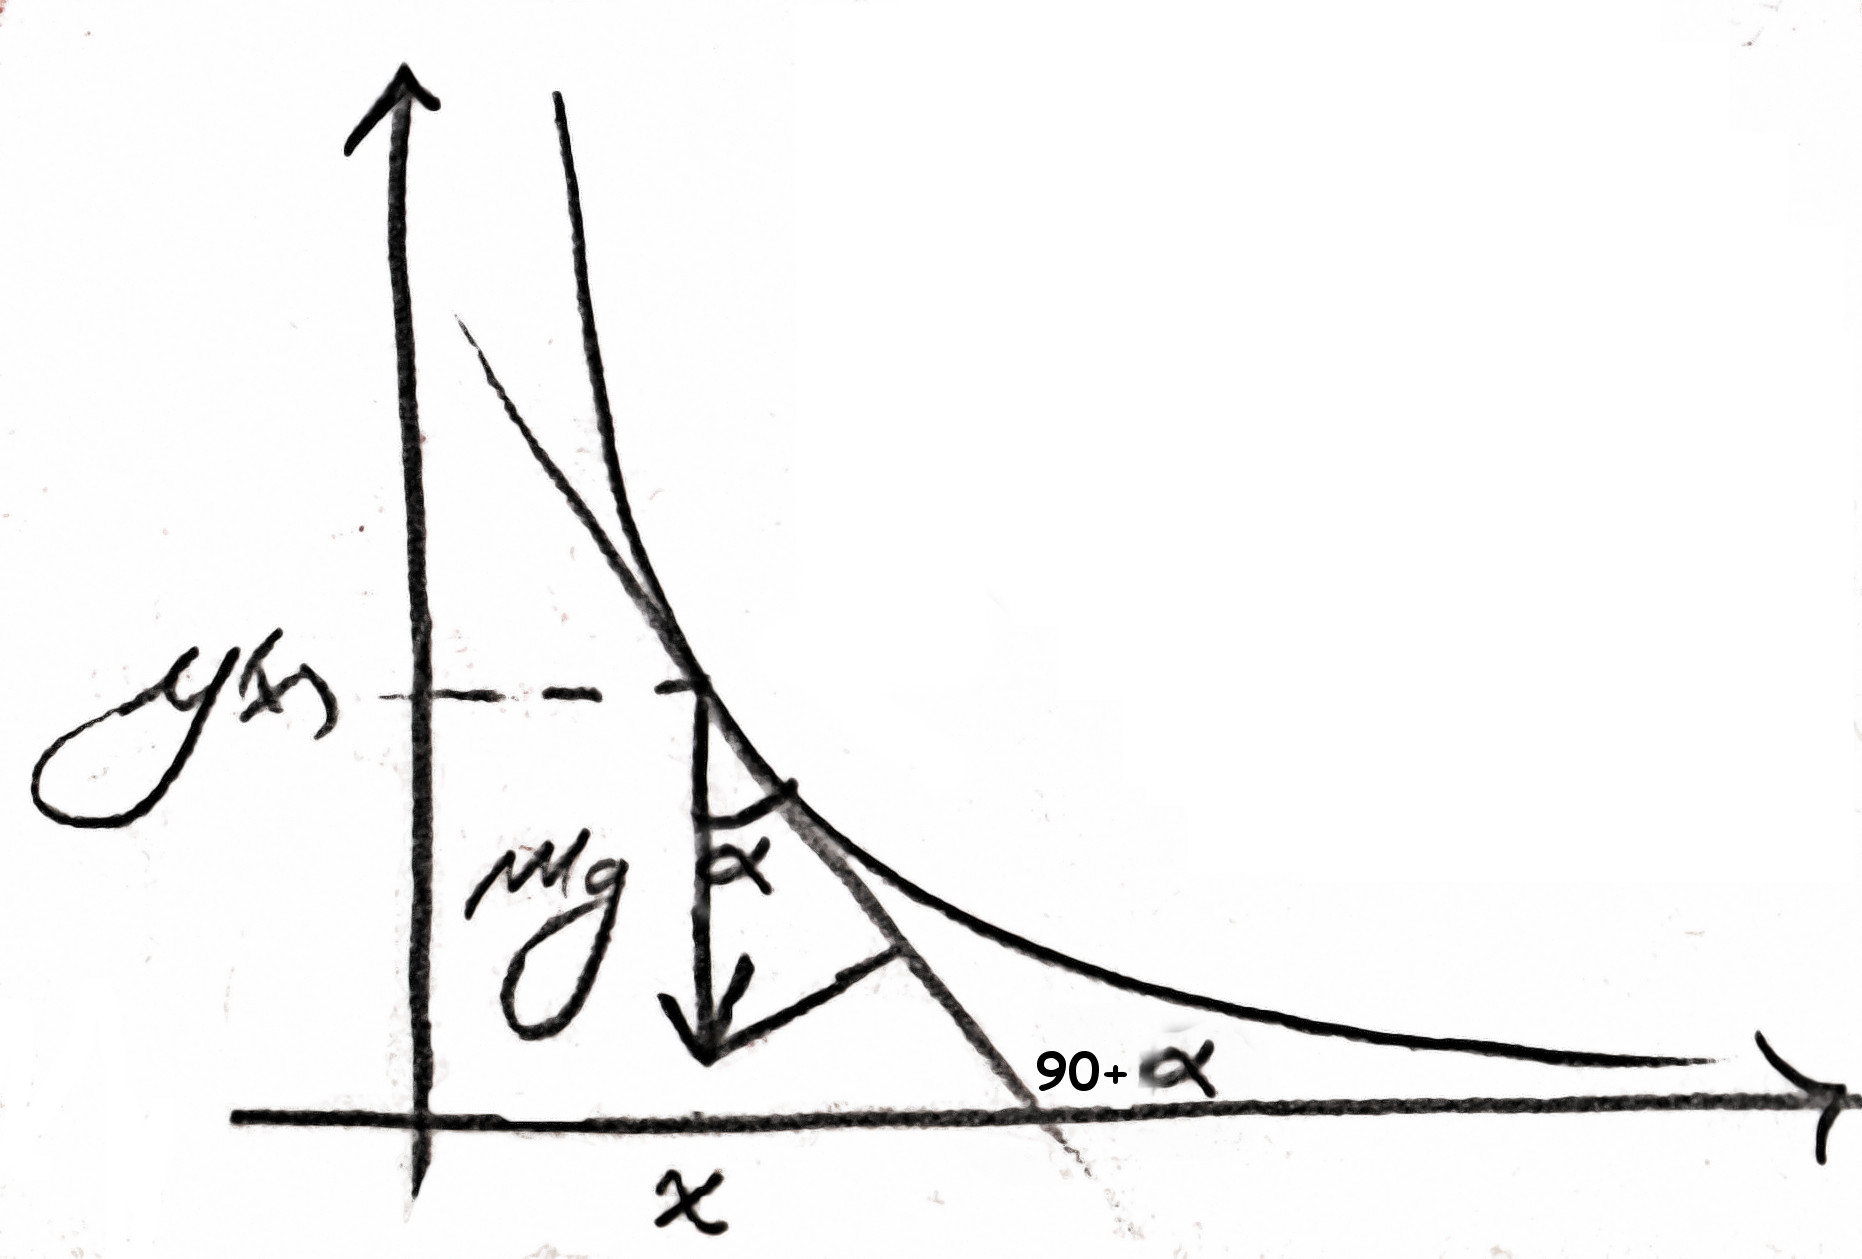
\includegraphics[scale=.07]{imagenes/caida_guia.jpg} & Supongamos que la guía esta
confinada a un plano. Introducimos un sistema de coordenadas ortogonales en dicho plano, con el suelo paralelo al eje $x$
\end{tabular}

El elemento longitud de arco $s$ de una curva que es el gráfico de una función $y(x)$ para $x$ en $[x_0,x_1]$ viene dado por 
\[s=\int_{x_0}^{x_1}\sqrt{1+y'(x)^2}dx\]
La fuerza de vínculo de la guía tiene componente tangencial nula,  la gravedad tiene una componente tangencial no nula. 
Su magnitud es $mg\cos\alpha$ (ver dibujo). Vamos a tratar de expresar $\cos\alpha$  en términos de   $y'(x)$. Vamos a suponer $\cos\alpha>0$ e $y'(x)<0$. 
Los demás casos quedan como \textbf{ejercicio}.
\[ \tan^2\alpha=\frac{\sen^2\alpha}{\cos^2\alpha}=\frac{1-\cos^2\alpha}{\cos^2\alpha}=\frac{1}{\cos^2\alpha}-1\]
y
\[y'(x)=\tan \left(\frac{\pi}{2}+\alpha\right)=-\frac{1}{\tan\alpha}\]
Podemos usar las relaciones anteriores para escribir $\cos\alpha$ en función de $y'(x)$
\begin{equation}\label{cos_alpha}\cos\alpha=-\frac{y'(x)}{\sqrt{1+y'(x)^2}}\end{equation}
Entonces
\begin{equation}\label{cons_ener}
 \begin{split} \frac{m}{2}|v(t_1)|^2-\frac{m}{2}|v(t_0)|^2&=\int_{s_0}^{s_1}f_tds =\int_{x_0}^{x_1}f_t\frac{ds}{dx}dx\\
&= -mg\int_{x_0}^{x_1}\frac{y'(x)}{\sqrt{1+y'(x)^2}}\sqrt{1+y'(x)^2}dx\\
&=-mg\left(y_1-y_0\right)
    \end{split}\end{equation}
Esto nos permite escribir la rapidez en función de la altura repecto al piso.




\begin{ejemplo}[Péndulo]
\end{ejemplo}

\noindent\begin{tabular}{m{6cm} m{5.5cm}}
  Se trata de una masa puntual $m$ suspendida de un punto por medio de una barra de longitud $l$
 a la que suponemos sin masa. Equivale al movimiento sobre una guía circular.  Usaremos el ángulo $\alpha$ marcado en la figura, como variable dependiente.
 & 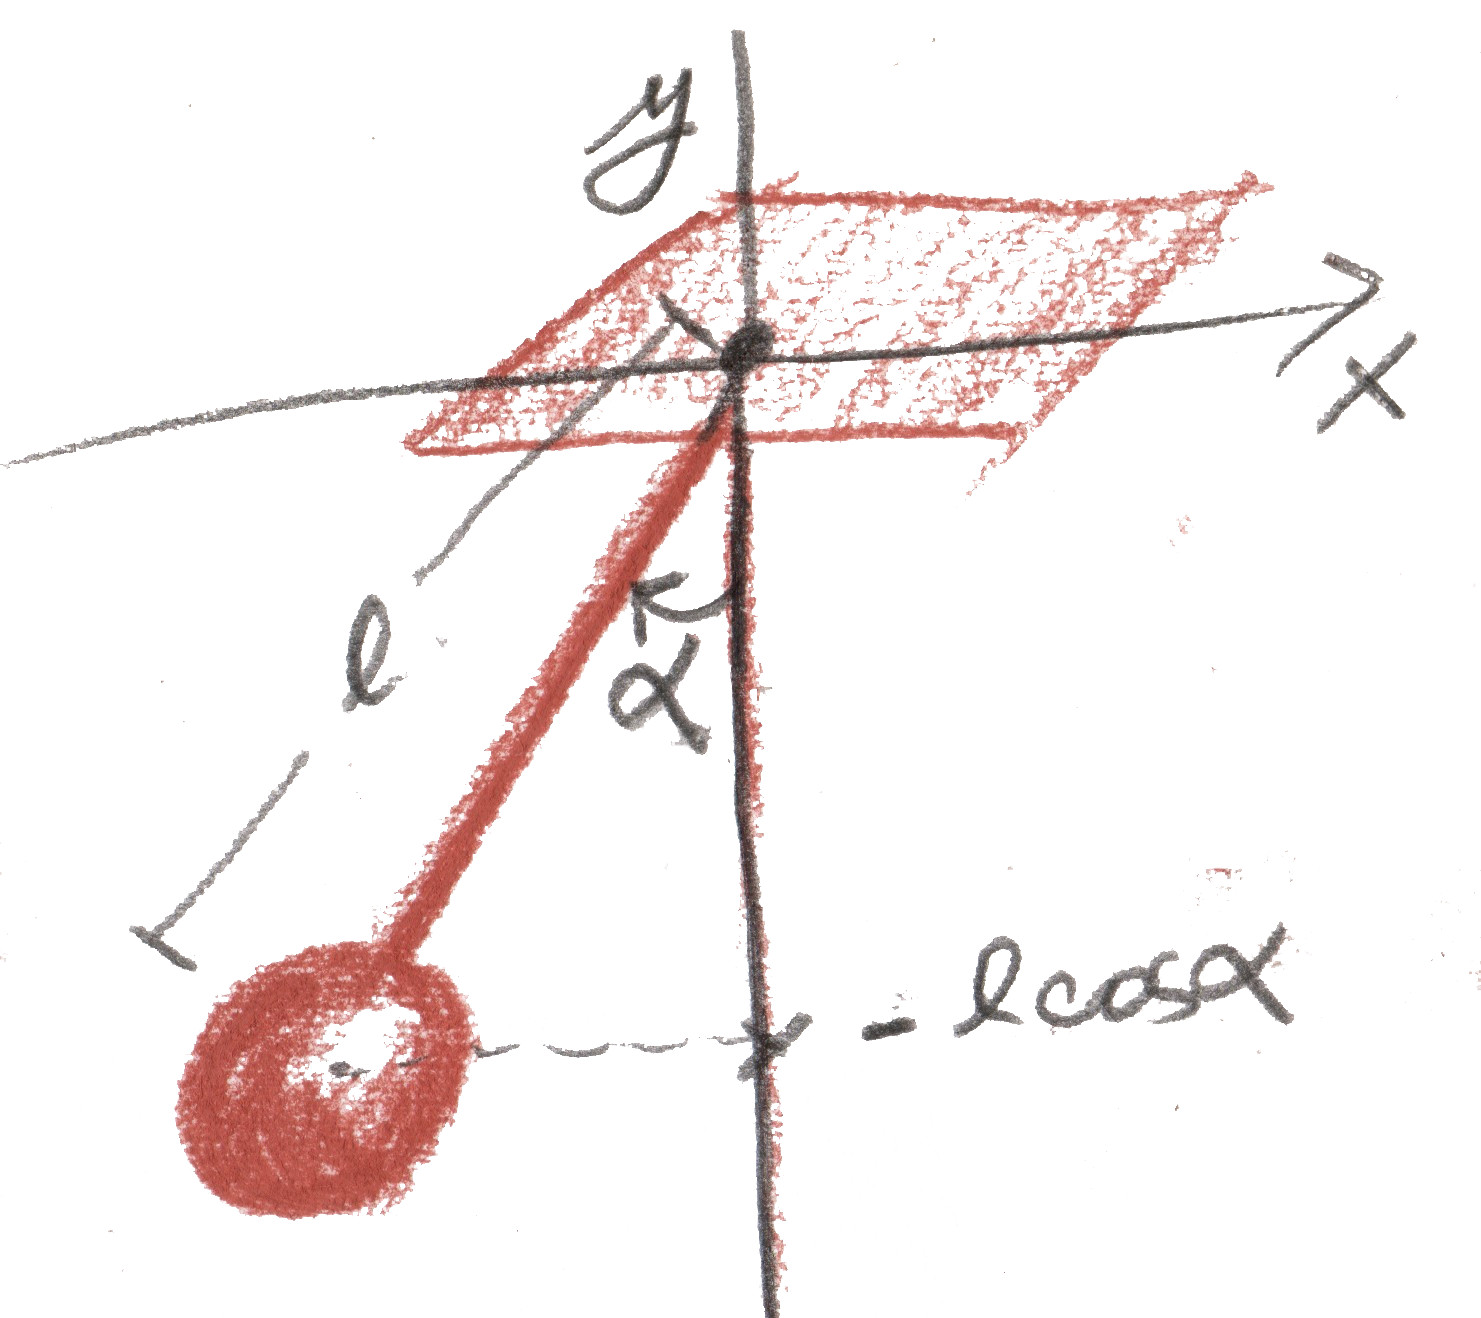
\includegraphics[scale=.07]{imagenes/pendulo.jpg} \\
\end{tabular}

Supondremos que el origen del sistema de de coordenadas está sobre el punto de amarre de la barra. Entonces de \eqref{cons_ener} con $t_1=t$ deducimos 
\[\begin{split}\frac{m|v(t)|^2}{2}-\frac{m|v(t_0)|^2}{2}&=-mg\left(y(t)-y(t_0)\right)\\
  &=mg\cos\alpha(t)-mg\cos\alpha(t_0).
   \end{split}
\]



Ahora la posición de la masa es $x(t)=l(\sen\alpha,-\cos\alpha)$ luego 
\[v(t)=l\alpha'(t)(\cos\alpha,\sen\alpha) \Longrightarrow |v(t)|^2=l^2\alpha'(t)^2.\]
Entonces
\[\frac{ml^2\alpha'(t)^2}{2}= mgl\cos\alpha(t)-mgl\cos\alpha(t_0) +\frac{mv(t_0)^2}{2}.\]
Derivando esta relación
\[ml^2\alpha'(t)\alpha''(t)=-mgl\alpha'(t)\sen\alpha(t).\]
De esto deducimos la ecuación del \href{http://es.wikipedia.org/wiki/Péndulo}{péndulo}
\[\boxed{\alpha''(t)=-\frac{g}{l}\sen\alpha(t)}.\]


\begin{ejemplo}[La braquistócrona]

\end{ejemplo}


\begin{problema} Dados dos puntos $A$ y $B$ en las proximidades de la superficie terrestre, uno mas abajo respecto al suelo que el otro,
queremos diseñar el tobogán óptimo entre los dos,
esto es el tobogán que nos lleve de $A$ hasta $B$ en el menor tiempo. La curva solución a este problema se llama curva 
\href{http://es.wikipedia.org/wiki/Curva_braquistócrona}{braquistócrona} (braquistos - el más corto, cronos - tiempo). 
\end{problema} \marginpar{\vspace{-30mm}
 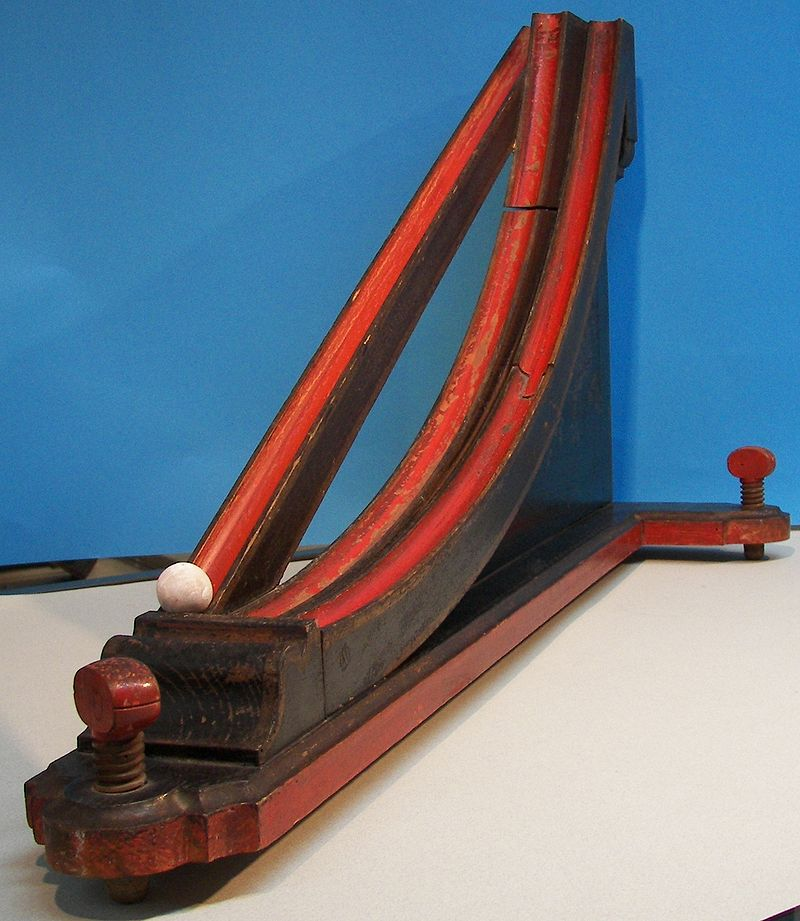
\includegraphics[scale=.07]{imagenes/braquis.jpg}
}
% \begin{center}


 Este problema fue resuelto por primera vez por Johann Bernoulli y es unos de los problemas precursores de la rama de las matemáticas que se denomina
\href{http://es.wikipedia.org/wiki/Cálculo_variacional}{cálculo de 
variaciones}. Vamos a dar la solución de Bernoulli que es muy elegante y está basada en un resultado de óptica llamado 
 el \href{http://es.wikipedia.org/wiki/Principio_de_Fermat}{Principio de Mínimo Tiempo} de \href{http://es.wikipedia.org/wiki/Fermat}{Fermat}.

\begin{boite}[boxcolor=orange, background=blue!5, titlebackground=blue!20,
titleboxcolor = black]{\href{http://es.wikipedia.org/wiki/Principio_de_Fermat}{\textbf {Principio de Mínimo Tiempo}} \textbf{de} \href{http://es.wikipedia.org/wiki/Fermat}{\textbf{Fermat}}}
 La luz sigue para ir de un punto a otro el recorrido que minimiza el tiempo.
\end{boite}



 La primera impresión   es que ese reccorrido debería ser la línea recta. Si embargo esto no es así debido a que la velocidad de la luz cambia
de acuerdo al \href{http://es.wikipedia.org/wiki/Velocidad_de_la_luz_en_un_medio_material}{medio que atraviesa}. 
La velocidad de la luz en el vacío es 299.792,458km/h y en el diamante 124.034,943 km/h. La velocidad de la luz cambia no sólo con la sustancia sino con sus cualidades, 
como la densidad. 

 Si la luz se mueve dentro de un medio homogéneo, el camino que sigue es la línea recta. Esto ya no es más así cuando la luz cambia de medio de propagación. Por ejemplo
cuando pasa del aire al vidrio. 


\begin{tabular}{m{4cm} m{7.5cm}}
 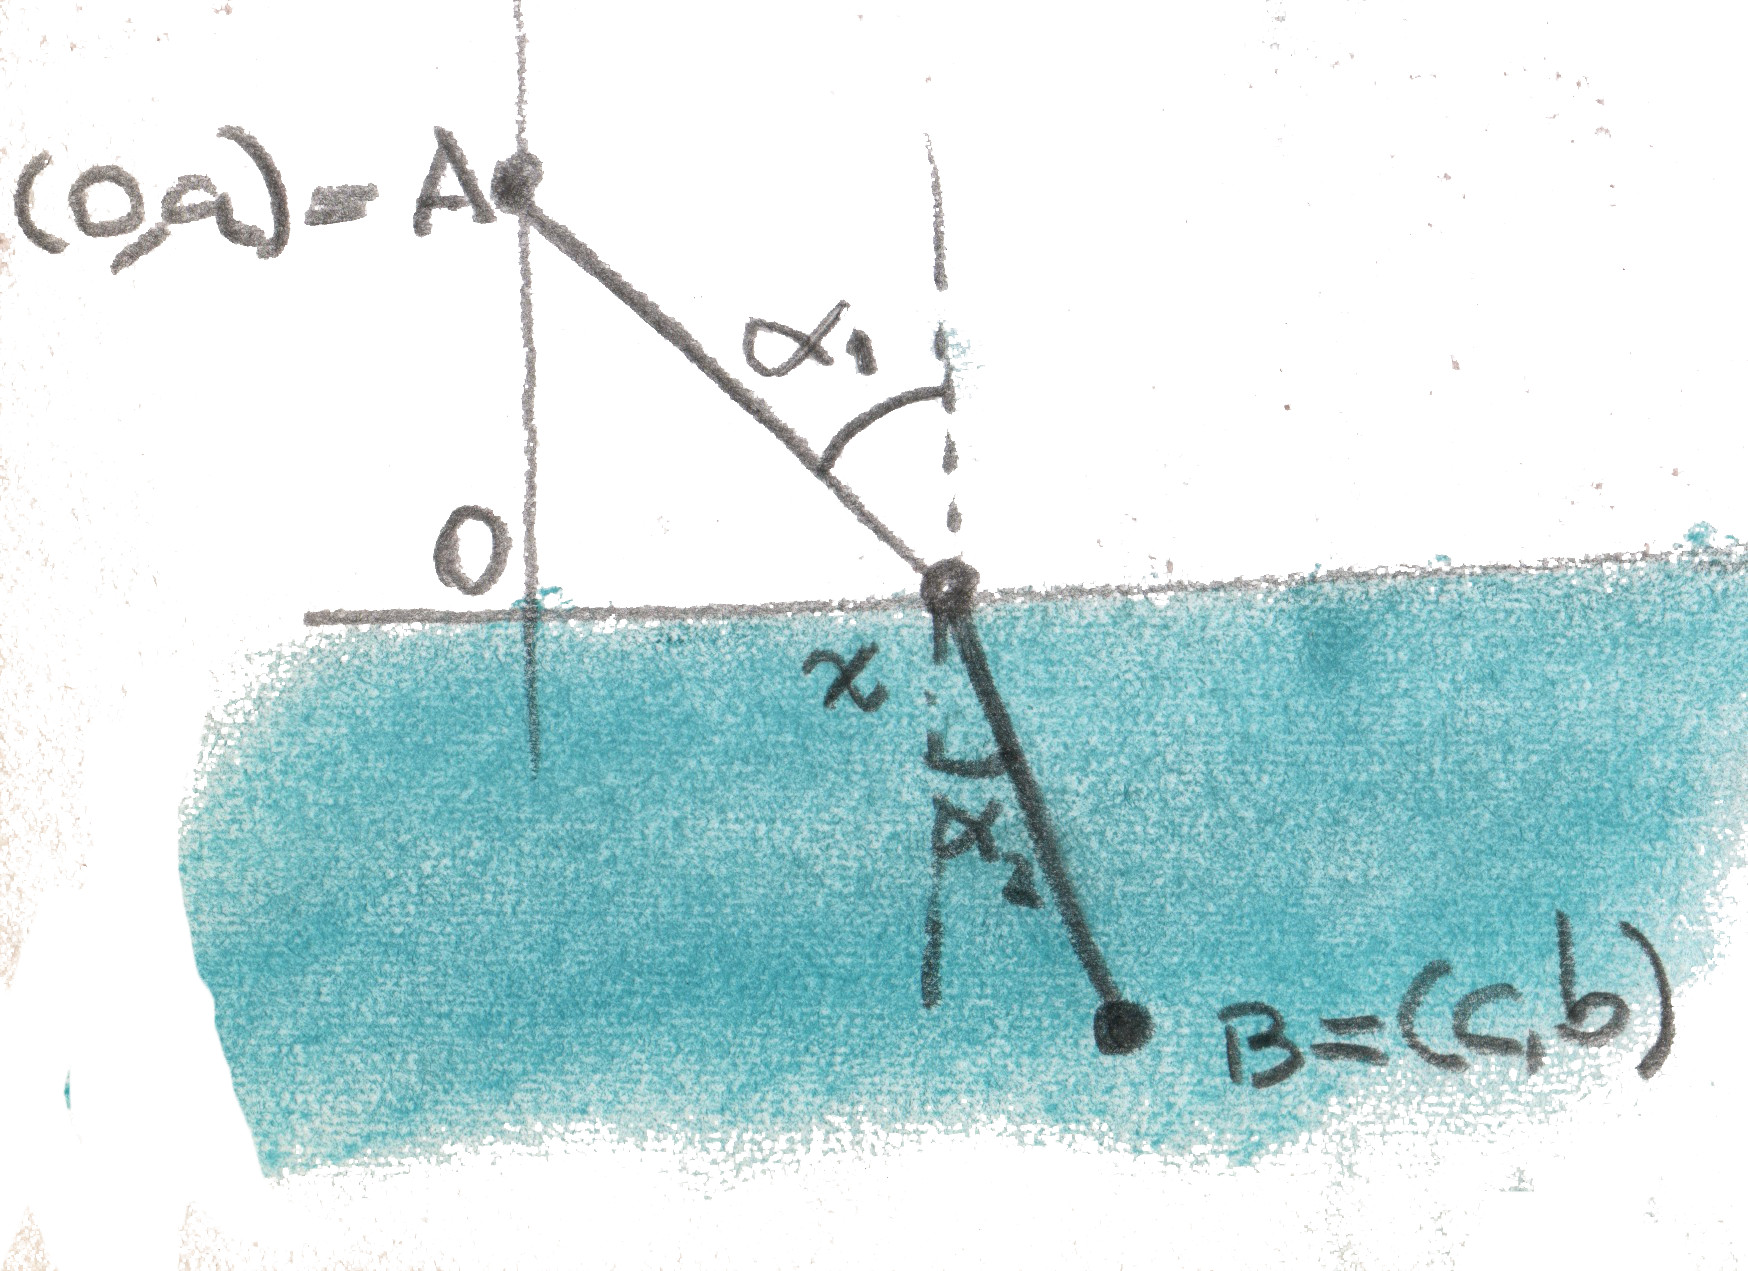
\includegraphics[scale=.07]{imagenes/refraccion.jpg} & Supongamos que la luz une los puntos $A$ y $B$ del plano y en el camino atravieza de un medio a otro, siendo la velocidad
 de la luz en cada uno de ellos $v_1$ y $v_2$.  Supongamos que $A=(a,0)$ y $B=(c,b)$ y el eje $x$ es la frontera entre los medios.
 \end{tabular}
Como sabemos que mientras se mueva en un medio homogéneo la luz sigue en línea recta,
el tiempo que emplea la luz para ir $A$ a $B$ es
 \[t=\frac{\sqrt{a^{2} + x^{2}}}{v_{1}} + \frac{\sqrt{{\left(c - x\right)}^{2} + b^{2}}}{v_{2}}\]
Para determinar la trayectoria es suficiente encontrar $x$, el punto donde la luz choca con la interfaz entre los medios. 
El principio de Fermat afirma que el tiempo es mínimo de modo que hallaremos un punto crítico de $t$ respecto a $x$. 
\[ \frac{dt}{dx}=-\frac{c - x}{\sqrt{{\left(c - x\right)}^{2} + b^{2}} v_{2}} +
\frac{x}{\sqrt{a^{2} + x^{2}} v_{1}}=\frac{\sen\alpha_1}{v_1}-\frac{\sen\alpha_2}{v_2} \]
Deducimos que en un punto crítico 
\boxedeq{\frac{\sen\alpha_1}{v_1}=\frac{\sen\alpha_2}{v_2} }{eq:ley_snell1}
que se denomina \href{http://es.wikipedia.org/wiki/Ley_de_Snell}{Ley de Snell}. El punto crítico es mínimo pues $\left.\frac{dt}{dx}\right|_{x=0}=-\tfrac{c}{bv_2}<0$ y
$\left.\frac{dt}{dx}\right|_{x=c}=\tfrac{c}{\sqrt{c^2+a^2}v_1}>0$.

 A la razón entre la velocidad de la luz dentro de un determinado medio y la velocidad de la luz en el vacio se lo denomina
\href{http://es.wikipedia.org/wiki/Índice_de_refracción}{índice de refracción} y se lo denota con la letra $n$. La Ley de Snell se la suele escribir
\[\boxed{n_1\sen\alpha_1=n_2\sen\alpha_2 }.\]
Que pasa si la luz atraviesa un medio que va cambiando de manera continua de índice de refracción. Por ejemplo, el índice de refracción en la atmósfera
va cambiando de manera continua con la altitud respecto a la superficie terrestre, ya que la densidad del aire va cambiando con la altitud. La Ley de
Snell en este caso es
\[\boxed{\frac{\sen\alpha}{v}=\text{cte}}\]
Aquí el ángulo $\alpha$ y la velocidad $v$ cambian respecto a alguna variable/s real/es, por ejemplo la altitud.


¿Que tienen en común el recorrido de la luz y la braquistócrona? Bernoulli se dió cuenta que la situación en los dos casos es la misma, ya que en los dos casos
se trata de minimizar el tiempo del recorrido. De modo que la braquistócrona también tiene que satisfacer la Ley de Snell.
 Ahora supongamos un sistema de coordenadas con origen en el punto $A$, inicial del recorrido.  Además supongamos que el movil  parte
del reposo. Con estas suposiciones $x(t_0)=0$ y $v(t_0)=0$. Por la conservación de la energía 
\[\frac{m}{2}|v(t)|^2=-mgy(t)=mg|y(t)|.\]
 Así por la ley de Snell
\[\frac{\sen\alpha}{|v(t)|}=\frac{\sen\alpha}{\sqrt{2g|y|}}=c=\text{ cte}.\]
En \eqref{cos_alpha} habíamos expresado el $\cos\alpha$ (en realidad del ángulo opuesto por el vértice, pero es igual) mediante la derivada. Luego
\[\sen\alpha=\sqrt{1-\cos^2\alpha}=\frac{1}{\sqrt{1+y'(x)^2}}.\]
Entonces tenemos
\[\sqrt{2g|y|}\sqrt{1+y'(x)^2}=c=\hbox{ cte}\]
Despejando llegamos a la ecuación diferencial
\[\boxed{\sqrt{\frac{y}{c-y}}y'=1}.\]
Es una ecuación con variables separables. La constante $c$ no tiene el mismo valor que en la ecuación anterior.  

La solución se obtiene resolviendo la integral
\[x=\int dx=\int \sqrt{\frac{y}{c-y}}dy.\]
lo que no es tan sencillo. Hacemos el cambio de variables
\[\sqrt{\frac{y}{c-y}}=\tan\phi\Longrightarrow y=c\sen^2\phi\Longrightarrow dy=2c\sen\phi\cos\phi d\phi.\]
Luego
\[x=2c\int\sen^2\phi d\phi=\frac{c}{2}\left(2\phi-\sen 2\phi\right)+C_1.\]
Como tiene que pasar por $x=0$ e $y=0$ debe ser $C_1=0$.  Tenemos que
 \[\left\{\begin{array}{l l l}
	      y&=c\sen^2 \phi&=\frac{c}{2}(1-\cos2\phi)\\
	      x&=\frac{c}{2}(2\phi-\sen2\phi)\ &\\
          \end{array}\right.
\]
Conviene llamar $2\phi=\theta$ y $a=c/2$
 \[\left\{\begin{array}{l l }
	      y&= a(1-\cos\theta)\\
	      x&=a(\theta-\sen\theta)\
          \end{array}\right.
\]
Que son la ecuaciones paramétricas de una curva conocida con el nombre de \href{http://es.wikipedia.org/wiki/Cicloide}{cicloide}. Podemos usar \texttt{SymPy} para graficar esta curva
\begin{lstlisting}
theta=symbols('theta')
from sympy.plotting import *
plot_parametric(theta-sin(theta),1-cos(theta),(theta,0,10*pi))
\end{lstlisting}

\begin{figure}[h]
\begin{center}
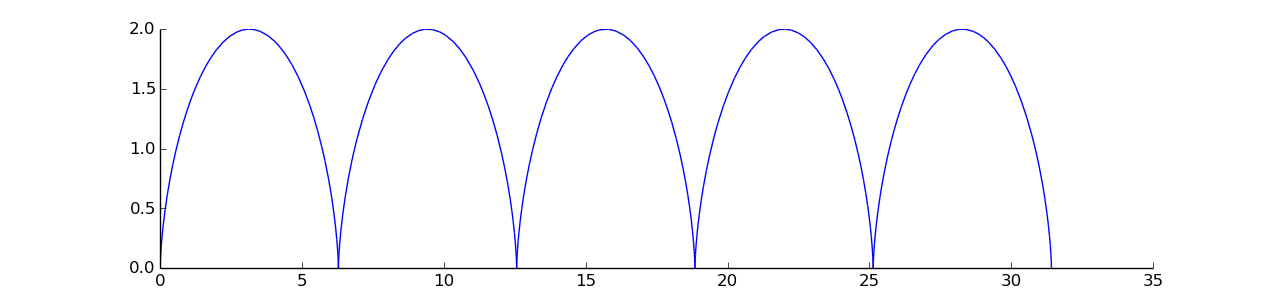
\includegraphics[scale=.3]{imagenes/cicloide.png}
\end{center}\caption{Cicloide}\label{fig:cicloide}
\end{figure}


Si in tentamos resolver las ecuaciones con \texttt{SymPy} el resultado no es muy alentador.

\begin{lstlisting}
x,c=symbols('x,c')
y=Function('y')(x)
MiEcua=Eq(y.diff(x),sqrt((c-y)/y))
f=dsolve(MiEcua,y,hint='separable')
\end{lstlisting}
\textbf{Resultado:}
\[
 \begin{cases} - i \sqrt{c} \sqrt{-1 + \frac{1}{c} y{\left (x \right )}} \sqrt{y{\left (x \right )}} - i c \operatorname{acosh}{\left (\frac{1}{\sqrt{c}} \sqrt{y{\left (x \right )}} \right )} & \text{for}\: \left\lvert{\frac{1}{c} y{\left (x \right )}}\right\rvert > 1 \\ \- \frac{\sqrt{c} \sqrt{y{\left (x \right )}}}{\sqrt{1 - \frac{1}{c} y{\left (x \right )}}} + c \operatorname{asin}{\left (\frac{1}{\sqrt{c}} \sqrt{y{\left (x \right )}} \right )} + \frac{y^{\frac{3}{2}}{\left (x \right )}}{\sqrt{c} \sqrt{1 - \frac{1}{c} y{\left (x \right )}}} & \text{otherwise} \end{cases} = C_{1} + x
\]




  \begin{ejemplo}[La tautócrona]


  \end{ejemplo}




  Vamos a ver otra propiedad notable de la ciclode. Supongamos que dejamos caer el cuerpo del reposo desde un punto intermedio, digamos en $(x_0,y_0)$. Sea  $\theta_0$
 el valor del paŕámetro $\theta$ correpondiente a este punto. ¿Cuánto tardara en llegar el cuerpo al punto mínimo de la curva que ocurre cuando $\theta=\pi$? 
% \begin{center}
% \animategraphics[controls,scale=.5]{15}{tautocrona/tauto-}{0}{79}
% \end{center}


  
  

 Tenemos
\[
 \left\{ \begin{array}{l l}
 \frac{dx}{d\theta}&=a(1-\cos\theta)\\
 \frac{dy}{d\theta}&=a\sen\theta 
 \end{array}\right.
\]
% 
Como el cuerpo ahora no parte de $(0,0)$ tendremos
\[|v|=\sqrt{2g(y_0-y)}.\]


  
  {La tautócrona}
Por \eqref{2ley} $ds/dt=|v|$. Si llamamos $T$ al tiempo que demanda en llegar a $\theta=\pi$, y llamamos  $s_0$ y $s_1$ a los arcos correspondientes al punto inicial
y final.  Tenemos
 \[T=\int_0^Tdt=\int_{s_0}^{s_1}\frac{dt}{ds}ds=\int_{s_0}^{s_1}\frac{1}{\sqrt{2g(y_0-y)}}ds.\]
Cambiando la variable de integración a $\theta$. Como 
\[
 \frac{ds}{d\theta}=\sqrt{\left(\frac{dx}{d\theta}\right)^2+\left(\frac{dy}{d\theta}\right)^2}=\sqrt{2}a\sqrt{1-cos\theta}.
\]
 Tenemos
\[T=\sqrt{\frac{a}{g}}\int_{\theta_0}^{\pi}\frac{\sqrt{1-\cos\theta}}{\cos\theta_0-\cos\theta}d\theta=
\sqrt{\frac{a}{g}}\int_{\theta_0}^{\pi}\frac{\sen\frac{\theta}{2}}{\cos^2\frac{\theta_0}{2}-\cos^2\frac{\theta}{2}}d\theta.
\]
Ahora hacemos la sustitución
\[u=\frac{\cos\frac{\theta}{2}}{\cos\frac{\theta_0}{2}}\Longrightarrow du=-\frac{\sen\frac{\theta}{2}}{2\cos\frac{\theta_0}{2}}d\theta.\]
Vemos que
\[
 T=2\sqrt{\frac{a}{g}}\int_0^1\frac{1}{\sqrt{1-u^2}}du.
\]
Que es una expresión independiente de $\theta_0$. En consecuencia el tiempo $T$ que demanda  el cuerpo para llegar $\theta=\pi$ es siempre el mismo no importa
desde donde se deje caer.



\end{document}
% \chapter{Teoría de Lie y ecuaciones diferenciales}

% 
\section{Introducción histórica}




\begin{quote}
<<Marius Sophus Lie fue un matemático noruego (17 de diciembre de 1842-18 de febrero de 1899) que creó en gran parte la teoría de la simetría continua, y la aplicó al estudio de la geometría y las ecuaciones diferenciales.
La herramienta principal de Lie, y uno de sus logros más grandes fue el descubrimiento de que los grupos continuos de transformación (ahora llamados grupos de Lie), podían ser
 entendidos mejor "linealizándolos", y estudiando los correspondientes campos vectoriales generadores (los, así llamados, generadores infinitesimales).
Los generadores obedecen una versión linealizada de la ley del grupo llamada el corchete o conmutador, y tienen la estructura de lo que hoy, en honor suyo, llamamos un álgebra de Lie.>>
\end{quote}
\marginpar{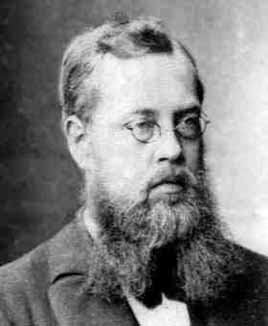
\includegraphics[scale=.28]{imagenes/Sophus_Lie.jpg}
}

\begin{flushright}
Wikipedia
\end{flushright}


 
\begin{quote}
<< La historia del análisis de simetrías comenzó a mediados del siglo XIX cuando S. Lie
Y F. Klein se reunieron en Berlín. Ambos matemáticos contribuyeron mucho a la teoría de las
simetrías. S. Lie presentó su famosa obra para examinar las simetrías en relación con
ecuaciones algebraicas y diferenciales. En su programa de Erlangen, Klein desarrolló las contrapartes discreta y algebraica de la aplicación de las simetrías a las funciones. S. Lie
creo un gran campo de las ecuaciones diferenciales, que fue muy útil para
clasificar las ecuaciones diferenciales de una forma nueva. La teoría desarrollada por Lie es
muy laboriosa, si se hace a mano. Esta es una de las razones por las que la aplicación de
esta teoría desapareció en la práctica de resolver problemas. Muy pocas personas usaron los procedimientos de  Lie para examinar ecuaciones diferenciales. Uno de ellos fue Birkhoff,
quien en la década de 1950 aplicó la teoría a problemas hidrodinámicos. En los últimos años,
 se prestó más atención a la teoría de Lie como uno de los métodos raros para obtener
soluciones, especialmente para ecuaciones diferenciales no lineales. Hoy el procedimiento de Lie es
accesible para su aplicación, si es usado el poder computacional del álgebra computacional. 
Los cálculos algebraicos muy extendidos hoy en día se llevan a cabo por computadoras. 
En los últimos 20 años, ha habido un enorme aumento de la potencia de  las computadoras y del desarrollo de lenguajes simbólicos, permitiendo abordar problemas en una
manera más sencilla.>>
\end{quote}
  

\begin{flushright}

Symmetry Analysis of
Differential Equations
with Mathematica\textregistered\\
\cite{GerdBaumann578}

\end{flushright}




\section{Cambios de Variables}



Vamos a seguir estudiando ecuaciones no lineales de primer orden

\boxedeq{\frac{dy}{dx}=f(x,y)}{eq:gral_orden1}
o, utilizando  la escritura en  \emph{forma diferencial}
\boxedeq{M(x,y)dx+N(x,y)dy=0.}{eq:gral_orden1_FormDif}
En el apéndice \ref{section:fromas} discutimos muy sumariamente el concepto de forma diferencial.

\begin{problema}[Cambio de variables]
 Dada la ecuación \eqref{eq:gral_orden1} o \eqref{eq:gral_orden1_FormDif} en las variables $x,y$. Queremos encontrar nuevas variables 
 \begin{equation}\label{eq:cambio_prin}
  \left \{\begin{array}{cc}
	    \hat{x}&=\hat{x}(x,y)\\
	    \hat{y}&=\hat{y}(x,y)
          \end{array}
 \right. .
 \end{equation}
tales que la ecuación se transforme en una que podamos resolver.
\end{problema}

Para no correr riesgos de perder información en la ecuación transformada, es conveniente que 
$x$ e $y$ también se expresan en función de $\hat{x}$ e $\hat{y}$, vale decir que la transformación pueda invertirse:
 \begin{equation}\label{eq:cambio_inv}
  \left \{\begin{array}{cc}
	    x&=x(\hat{x},\hat{y})\\
	    y&=y(\hat{x},\hat{y})
          \end{array}
 \right. .
 \end{equation}
\subsection{Cómputos de cambios de variables}\marginpar{Es costumbre recurrir a un abuso de notación que suele producir confusión al estudiante. Nos referimos a distinguir las derivadas $\partial y/\partial x$ y  $d y/d x$. Tratándose $y$ en el caso que nos ocupa, de una función de $x$ e $\hat{y}$,    la derivada $\partial y/\partial x$ representa la derivada parcial de $y$ respecto a su primera variable. Como $\hat{y}$ es a su vez función de $x$, por  $d y/d x$ denotamos la derivada de $y$ atendiendo a que la segunda variable también depende de $x$.}
Vamos a estudiar en primer lugar como computar cambios de variables. Empezaremos por casos más sencillos hasta ir a la situación más general.

\subsubsection{Cambio de la variable dependiente manteniendo la independiente}

 Supongamos que el conjunto de variables se relacionan  por las identidades $x=\hat{x}$ e  $y=y(x,\hat{y})$. Notar que en este caso usamos la relación inversa. Entoces, derivando $y$ respecto a $x$ y usando la regla de la cadena (que sería más apropiado llamarla regla de cambio de variables para la derivada)

\[\frac{dy}{dx}=\frac{\partial y}{\partial x}+\frac{\partial y}{\partial \hat{y}}\frac{d\hat{y}}{dx}.\]

La ecuación se convierte

\[\frac{\partial y}{\partial x}+\frac{\partial y}{\partial \hat{y}}\frac{d\hat{y}}{dx}=f(x,y(x,\hat{y})).\]
Que es una expresión sólo en $\hat{y}$ y $x$. Parece más complicada, pero en un ejemplo concreto puede ser más simple.







\begin{ejemplo}{} Hacer el cambio de variable propuesto en la  ecuación indicada
\[y=\frac{e^{\hat{y}}}{x}\quad\text{en}\quad  y'=\left[\ln(xy)\right]^2xy-\frac{y}{x}.\]
 1) Expresemos $dy/dx$ sólo con $x$, $\hat{y}$ y $d\hat{y}/dx$.
\[\frac{dy}{dx}=-\frac{e^{\hat{y}}}{x^2}+\frac{e^{\hat{y}}}{x}\frac{d\hat{y}}{dx}.\]
 2) Remplacemos $y'$ e $y$ en la ecuación
\[-\frac{e^{\hat{y}}}{x^2}+\frac{e^{\hat{y}}}{x}\frac{d\hat{y}}{dx}=\left[\ln\left(x \frac{e^{\hat{y}}}{x} \right)\right]^2x\frac{e^{\hat{y}}}{x}-\frac{\frac{e^{\hat{y}}}{x} }{x}.\]
 3) Simplifiquemos
\boxedeq{\frac{d\hat{y}}{dx}=\hat{y}^2x.}{}




\end{ejemplo}

  \emph{Importante:} Observar  que en un cambio de variable, ya se cambie la variable dependiente, independiente o ambas, las derivadas (tratándose de la velocidad de cambio de unas variables repecto a otras)  también hay que cambiarlas.


Podemos resolver los cambios de variables con \texttt{SymPy}, lo cual es muy útil por dos motivos. El primero porque nos permite hacer cambios de variables en expresiones muy grandes, resolviendo operaciones que a mano son sumamente tediosas. El segundo, y no menos importante para nosotros, es que es muy rico explorar un procedimiento enmarcándolo en un contexto muy distinto. En este caso, el procedimiento es relizar un cambio de variables y estamos explorando el mismo a través de un breve código que lo implementa en un lenguaje de programación.

\begin{sympyblock}[][frame=single]
from sympy import *
x=symbols('x') #unico simbolo primitivo
y_n=Function('y_n')(x) #variables nuevas, funciones de x
y=exp(y_n)/x #relacion entre y, y_n
eq=Eq(y.diff(x)-(ln(x*y))**2*x*y+y/x,0) #la ecuacion
eq1=simplify(eq) # simplifica expresiones
\end{sympyblock}
Obtenemos la ecuación

\[\sympy{eq1},\]
que \texttt{SymPy} no simplifica a nuestro gusto

% 
% 
% 
\subsubsection{Cambio de la variable independiente manteniendo la dependiente}

Supongamos  $\hat{x}=\hat{x}(x)$. Usamos la relación
\[\frac{dy}{dx}=\frac{dy}{d\hat{x}}\frac{d\hat{x}}{dx}.\]
Suponiendo que la relación $\hat{x}=\hat{x}(x)$ se invierte en $x=x(\hat{x})$, todo lo que resta es sustituir  $x$ por su igual en términos de $\hat{x}$

\[\frac{dy}{d\hat{x}}=f(x(\hat{x}),y) \left[\left.\frac{d\hat{x}}{dx}\right|_{x=x(\hat{x})}\right]^{-1}.\]
Que es una expresión sólo en $\hat{x}$ e $y$. Describir el procedimiento  en general puede hacer parecer que es más dificil de lo que en realidad es en un caso concreto.



\begin{ejemplo}{} Hacer el cambio de variable en la  ecuación indicados
\[x=\cos \hat{x}\quad\text{en}\quad  -\frac{dy}{dx}+\frac{x}{\sqrt{1-x^2}}y=0.\]
1) $\hat{x}=\arcsen x$
\[\frac{dy}{dx}=\frac{dy}{d\hat{x}} \frac{d\hat{x}}{dx}  =-\frac{1}{\sqrt{1-x^2}}\frac{dy}{d\hat{x}}.\]
 2) Remplacemos $x$ e $y'$ en la ecuación
\[\frac{1}{\sqrt{1-x^2}}\frac{dy}{d\hat{x}}+ \frac{x}{\sqrt{1-x^2}}y=0\]
3) Reemplazando $x$ por $\cos(\hat{x})$ y simplificando
\[\frac{dy}{d\hat{x}}+\cos(\hat{x}) y=0.\]

\end{ejemplo}


Para hacer esto con \texttt{SymPy} (de ahora en más omitiremos la sentencia de importanción del módulo, esta operación se hace sólo una vez por sesión).

\begin{sympyblock}[][frame=single]
x=symbols('x')
x_n=acos(x)
y=Function('y')(x_n)
Ecuacion=-y.diff()+1/(sqrt(1-x**2))*y
xn=symbols('xn')
Eq=Ecuacion.subs(x,cos(xn))
\end{sympyblock}

Obtenemos la ecuación

\[\sympy{Eq}\]

hola

Nuevamente \texttt{SymPy} no simplifica a nuestro gusto, esto ocurre aún con aquellas expresiones que parece muy evidente como se simplifican. El caso es que la operación de simplificación es por un lado  subjetiva, depende de un supuesto tácito de a que expresión se quiere arribar y por otro algunas expresiones, por ejemplo $\ln\exp(z)$, se simplifican en determinados campos numéricos y en otros no. En el caso del ejemplo $\ln\exp(z)$, la expresión es simplificable si $z\in\rr$, pero no lo es si por ejemplo $z\in\mathbb{C}$. De modo que no puede esperarse que Sympy efectúe esta simplificación a menos que conozca que se trabaja en el campo numérico indicado. Hay que distinguir que supuestos tácitos está haciendo uno y hay que indicarselos a Sympy.    El lector debe tener en cuenta que en ningún momento uno le dijo a \texttt{SymPy} que tipo de ente estaba manipulando en expresiones del tipo \texttt{x\_n=acos(x)}. Puede parecer natural que se trata de números reales, no obstante esta 
información nunca fue comunicada al interprete de \texttt{SymPy}. ¿Porqué el habría de entender que \texttt{x} es real? Si al fin y al cabo \texttt{x\_n=acos(x)} tiene sentido si \texttt{x} es complejo y aún si es una matríz. Muchas veces las operaciones que se simplifican en un campo no lo pueden hacer en otro. El comando  \texttt{symbols} tiene la opción de informar a \texttt{SymPy} que tipo de ente representa \texttt{x} de la siguiente forma
\texttt{x=symbols('x',real=True)}. De esta forma se consiguen mejores resultados en las simplificaciones.


\subsubsection{Cambio de variable general $\hat{x}=\hat{x}(x,y)$, $\hat{y}=\hat{y}(x,y)$}
\begin{enumerate}
  \item Calculamos $d\hat{y}/d\hat{x}$ en las variables $x,y$
    \boxedeq{
      \frac{d\hat{y}}{d\hat{x}}=\frac{\frac{d\hat{y}}{dx}}{\frac{d\hat{x}}{dx}}=\frac{\frac{\partial\hat{y}}{\partial x}+\frac{\partial\hat{y}}{\partial y}y'}{\frac{\partial\hat{x}}{\partial x}+\frac{\partial\hat{x}}{\partial y}y'}=\frac{\frac{\partial\hat{y}}{\partial x}+\frac{\partial\hat{y}}{\partial y}f(x,y)}{\frac{\partial\hat{x}}{\partial x}+\frac{\partial\hat{x}}{\partial y}f(x,y)}.
	    }{eq:subsder}

   \item En la expresión resultante sustituímos $x,y$ por las tansformaciones 			inversas $x=x(\hat{x},\hat{y})$ y  $y=y(\hat{x},\hat{y})$
\end{enumerate}



\begin{ejemplo}{ej:cambio_forma} Transformar a polares
 \[
  \frac{dy}{dx}=\frac{y^3+x^2y-x-y}{x^3+xy^2-x+y}.
 \]
\end{ejemplo}

Dado que el cálculo es extenso lo haremos con \texttt{SymPy}, el procedimiento seguido ilustra como hacerlo a mano. Es ilustrativo hacer esto último para apreciar la utilidad de usar un sistema de álgebra computacional (SAC) como \texttt{SymPy}.

\begin{sympyblock}[][frame=single]
x=symbols('x')
y=Function('y')(x)
r=sqrt(x**2+y**2)
theta=atan(y/x)
Expr2=r.diff(x)/theta.diff(x)
\end{sympyblock}



Obtenemos la siguiente expresión 
\[\sympy{Expr2}.\]
Ahora sustituímos $y'(x)$ usando la ecuación diferencial, redefinimos $r,\theta$ fundamentalmente para limpiar el valor que tenían asignado en el código previo, que era una expresión de $x,y$, y finalmente sustituímos $x$ e $y$ por su expresión en polares.

\begin{sympyblock}[][frame=single]
Expr3=Expr2.subs(y.diff(x),(y**3+x**2*y-x-y)/(x**3+x*y**2-x+y))
r,theta=symbols('r,theta',positive=True)
Expr4=Expr3.subs([(y,r*sin(theta)),(x,r*cos(theta))])
Expr5=simplify(Expr4)
\end{sympyblock}


 Encontramos que en polares la ecuación es mucho más simple
\[\frac{dr}{d\theta}=-r^3+r.\]

 Quizás  usar la notación como  forma diferencial sea más efectivo. Como $r$ y $\theta$ son funciones de $x$ e $y$, ellas son 0-formas. Usando las reglas de la diferencial, hay que reemplazar
\[
\begin{array}{ll}
x=r\cos\theta; &dx=\cos\theta dr-\sen\theta r d\theta\\
 y= r\sen\theta; & dy=\sen\theta dr+\cos\theta r d\theta\\
\end{array}
\]
en la 1-forma:
\[(y^3+x^2y-x-y)dx-(x^3+xy^2-x+y)dy.\]

Sympy posee un módulo para operar con formas diferenciales, en un apéndice describimos como utilizarlo para resolver este ejemplo.

\section{Grupos}

\marginpar{Las raíces históricas de la teoría de grupos son la teoría de las ecuaciones algebraicas, la teoría de números y la geometría. Euler, Gauss, Lagrange, Abel y Galois fueron los creadores que ponen los cimientos de esta rama del álgebra abstracta.  Otros importantes matemáticos que contribuyen son Cayley, Emil Artin, Emmy Noether, Peter Ludwig Mejdell Sylow, A.G. Kurosch, Iwasawa entre muchos otros.
\raggedright{(Wikipedia)}
}
 \subsection{Definición y ejemplos}
\begin{definicion}[Grupo]
Un \href{https://es.wikipedia.org/wiki/Grupo_(matem%C3%A1tica)}{grupo} es un par $(G,\cdot)$ donde $G$ es un conjunto y $\cdot :G\times G\to G$ una \href{https://es.wikipedia.org/wiki/Operaci%C3%B3n_matem%C3%A1tica}{operación binaria interna} que satisface
\begin{enumerate}
\item $(g_1\cdot g_2)\cdot g_3=g_1\cdot (g_2\cdot g_3)$, para todos $g_1,g_2,g_3\in G$,
\item Existe $e\in G$ tal que $e\cdot g=g\cdot e=g$,  para todo $g\in G$.
\item Para todo $g\in G$ existe $h\in G$ tal que $g\cdot h=h\cdot g=e$. Esta función $h$ se denota  $g^{-1}$.
\end{enumerate}
\end{definicion}

Es usual omitir el punto para indicar la operación, i.e. escribimos $g\cdot h=gh$.



\begin{ejemplo}{} Sea $\Pi$ un plano euclideano y $G$ el conjunto de todas las transformaciones rígidas de $\Pi$ en si mismo. Entonces $G$ es un grupo con la operación de composición. Se llama el \emph{grupo de transformaciones rígidas}.
 \end{ejemplo}


\begin{ejemplo}{}  Sea $X=\{x_1,\ldots,x_n\}$ un conjunto de $n$ elementos y $S_n$ definido por
\[S_n=\{\sigma|\sigma:X\to X\hbox{ y }\sigma \hbox{ es biyectiva }\}\]
Entonces $S_n$ es un grupo  con la operación de composición. Se denomina \href{http://es.wikipedia.org/wiki/Grupo_simétrico}{\emph{grupo simétrico}}.
 \end{ejemplo}

\begin{ejemplo}{} Sea $\Delta$ un polígono regular de $n$ lados  en un plano euclideano $\Pi$ y $D_{2n}$ el conjunto de todas las transformaciones rígidas de $\Pi$ en si mismo que llevan $\Delta$ en si mismo. $D_{2n}$ se llama el \href{http://es.wikipedia.org/wiki/Grupo_diedral}{\emph{grupo diedral}}  de orden $2n$. Para un triángulo equilatero:
\begin{center}
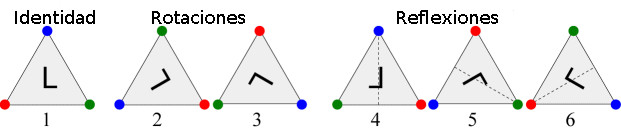
\includegraphics[scale=.4]{imagenes/SimTria.jpg}
\end{center}
\end{ejemplo}

Recordemos el siguiente concepto.

\begin{definicion}[Acción de un grupo sobre un conjunto]
Diremos que un grupo $G$ actúa sobre el conjunto $X$ si existe una operación binaria externa  $\star:G\times X\to G$ que satisface:
\begin{enumerate}
\item Si $e$ es el neutro de $G$, $e \star x=x$,  para todo $x\in X$.
\item Para todos $g,h\in G$ y $x\in X$,    $g\star (h\star x)=(gh)\star x$.
\end{enumerate}
\end{definicion}

Como en el caso de grupos suele nos escribirse el símbolo de la operación binaria, i.e. se escribe $g\star x= gx$.




\section{Grupos continuos de simetrías}

\subsection{Grupos y cambios de variables}

Los cambios de variables de un conjunto de dos variables, digamos $x$ e $y$, son funciones $\Gamma$, invertibles,  de clase $C^1$, donde $\Gamma:\Omega_1\to\Omega_2$, con $\Omega_1,\Omega_2$ abiertos de $\rr^2$.  Acostumbraremos escribir $(\hat{x},\hat{y})=\Gamma(x,y)$ y diremos que $(\hat{x},\hat{y})$ son la variables nuevas y $(x,y)$ las viejas.

\begin{ejemplo}{} \textbf{Coordenadas polares.} Es más facil describir la transformación que lleva coordenadas polares en cartesianas. En este caso $(x,y)=\Gamma(r,\theta)$ y
\[
\begin{array}{ll}
\Gamma(r,\theta)&=(r\cos(\theta),r\sen(\theta)),\\
\Omega_1&=(0,\infty)\times (-\pi,\pi),\\
\Omega_2&=\rr^2-\{(x,y)|y=0,x\leq 0\}\\
\end{array}
\]
\end{ejemplo}

\subsection{Grupos de Lie uniparamétricos}

\begin{definicion}[Grupos de Lie uniparamétricos]  Supongamos dada una acción del grupo  $(\rr,+)$ en $\rr^2$. En este caso vamos a adoptar una notación funcional, i.e. en lugar de escribir $\epsilon\star (x,y)$, con $\epsilon\in\rr$ y $(x,y)\in\rr^2$ pondremos $\Gamma_{\epsilon}(x,y)$. Denotaremos por $\{\Gamma_{\epsilon}\}$ a la acción introducida.  Notar que $\{\Gamma_{\epsilon}\}$  satisface que 
\begin{enumerate}
 \item $\forall\epsilon_1,\epsilon_2\in\rr:\Gamma_{\epsilon_1}\circ \Gamma_{\epsilon_2}=\Gamma_{\epsilon_1+\epsilon_2}$.

\item $\Gamma_0=I$.

\item $\Gamma_{\epsilon}$ es invertible y $\left(\Gamma_{\epsilon}\right)^{-1}=\Gamma_{-\epsilon}$
\end{enumerate}

La acción $\Gamma_{\epsilon}$ se denomina un  \href{http://es.wikipedia.org/wiki/Grupo_uniparamétrico}{\emph{grupo de Lie uniparamétrico}} si además:

\begin{enumerate}
\item[4.] $\forall\epsilon\in\rr:\Gamma_{\epsilon}$ es un difeomorfismo sobre $\rr^2$.


\item[5.] Si $\Gamma_{\epsilon}(x,y)=\left(\hat{x}(x,y,\epsilon),\hat{y}(x,y,\epsilon)\right)$ entonces   las funciones  $\hat{x}(x,y,\epsilon)$ y $\hat{y}(x,y,\epsilon)$  se desarrollan en serie de potencias respecto a $\epsilon$. Es decir para todo $\epsilon_0\in\rr$ existen coeficientes $a_j$ y $b_j$, $j=0,1,\ldots$, y $r>0$ tales que
\begin{equation}\label{eq:des_serie}
\begin{array}{cc}
\hat{x}(x,y,\epsilon)&=a_0(x,y)+a_1(x,y)(\epsilon- \epsilon_0)+\cdots\\
\hat{y}(x,y,\epsilon)&=b_0(x,y)+b_1(x,y)(\epsilon- \epsilon_0)+\cdots\\
\end{array}
\end{equation}
para $|\epsilon-\epsilon_0|<r$.
\end{enumerate}
\end{definicion}



\begin{ejemplo}{} Demostrar que las siguientes aplicaciones inducen grupos de Lie uniparamétricos
\begin{enumerate}
\item $\Gamma_{\epsilon}(x,y)=(x+\epsilon,y)$ y $\Gamma_{\epsilon}(x,y)=(x,y+\epsilon)$.
\item $\Gamma_{\epsilon}(x,y)=(e^{\epsilon}x,y)$
\item$\Gamma_{\epsilon}(x,y)=\left(\frac{x}{1-\epsilon x},\frac{y}{1-\epsilon x} \right)$
\item$\Gamma_{\epsilon}(x,y)=\begin{pmatrix} \cos(\epsilon) & -\sen(\epsilon)
\\ \sen(\epsilon) & \cos(\epsilon)
\end{pmatrix} \begin{pmatrix} x\\ y
\end{pmatrix}
$
\end{enumerate}
\end{ejemplo}

Vamos a desarrollar sólo el ejemplo de $\Gamma_{\epsilon}(x,y)=(x+\epsilon,y)$. La propiedad 1 en la definición la chequearemos con  \texttt{SymPy}. 

\begin{sympyblock}[][frame=single]
x,y,epsilon,epsilon1,epsilon2=symbols('x,y,epsilon,epsilon1,epsilon2')
T=Matrix([x+epsilon,y])
x_copete=T.subs(epsilon,epsilon1)[0]
y_copete=T.subs(epsilon,epsilon1)[1]
PropGrupo=T.subs([(x,x_copete),(y,y_copete),(epsilon,epsilon2)])\
-T.subs(epsilon,epsilon1+epsilon2)
\end{sympyblock}

\[\sympy{PropGrupo}.\]


 La propiedad 2 en la definición es evidente y la propiedad 3 es siempre consecuencia de 1. y 2. 
Se incluyó en la lista sólo para resaltar su cumplimiento, pero no es necesario chequearla. La propiedad 4. es clara la 5. también lo es, notar que el desarrollo en serie \eqref{eq:des_serie} es válido en este caso con $a_0(x,y)=x$, $a_1(x,y)=1$, $a_j(x,y)=0$, $j\geq 2$, $b_0(x,y)=y$ y $b_j(x,y)=0$, $j\geq 1$. La justificaciones correspondientes al resto de los ejemplos queda como ejercicio.


 Las reflexiones en el plano, por ejemplo $\Gamma(x,y)=(-x,y)$,  no pueden  pertenecer a un  grupo de Lie uniparamétrico. Más generalmente:
 
 \begin{teorema}{}
   Una transformación  $T:\rr^2\to\rr^2$ tal que el determinante de la matriz Jacobiana $\det(DT)$ sea negativo en algún punto no puede pertenecer a un grupo de Lie uniparamerico. Dicho de otro modo, debe ocurrir que $\det(D\Gamma_{\epsilon})>0$ para todo $\epsilon$ y todo grupo $\{\Gamma_{\epsilon}\}$.
 \end{teorema}
\begin{proof}
 Si $\Gamma_{\epsilon}$ es un grupo y supongamos por ejemplo que existe $\epsilon_0\in\rr$ y $(x_0,y_0)\in\rr^2$ tal que:

\[J(x_0,y_0,\epsilon_0):=\det\begin{pmatrix} \frac{\partial\hat{x}}{\partial x}&  \frac{\partial\hat{x}}{\partial y}\\
 \frac{\partial\hat{y}}{\partial x} &  \frac{\partial\hat{y}}{\partial y}\\
\end{pmatrix}<0,
\]
donde las derivadas son tomadas en $\epsilon=\epsilon_0, x=x_0$ y $y=y_0$.
 Por otro lado tenemos que $J(x_0,y_0,0)=1$. Como $J(x_0,y_0,\epsilon)$ es continua respecto a $\epsilon$ debería existir $\epsilon'$ con $J(x_0,y_0,\epsilon')=0$. Esto implica que la matriz jacobiana $D\Gamma_{\epsilon}$ es singular y esto contradice que $\Gamma:\rr^2\to \rr^2$ es difeomorfismo ($D\Gamma D\Gamma^{-1}=I$).
\end{proof}


 
 
 



 En el caso de la reflexión $\Gamma(x,y)=(x,-y)$, se  genera un grupo discreto, ya que $\Gamma^2=\Gamma\circ \Gamma=I$. Luego $\Gamma$ genera el grupo finito $G=\{I,\Gamma\}$ que es isomorfo a $\mathbb{Z}_2$. En este caso diremos que    $\{I,\Gamma\}$ es un \emph{grupo discreto}.





\subsection{Grupos de simetrías de EDO}
\begin{definicion}[Grupo de simetrías de una ecuación]
 Consideremos una ecuación
\boxedeq{y'=f(x,y).}{eq:principi}
Una transformación o cambio de variables $\Gamma$ se denomina una \emph{simetría} de la ecuación si el cambio de variables dado por $(\hat{x},\hat{y})=\Gamma(x,y)$ deja invariante  la ecuación.  Diremos que un grupo de Lie uniparamétrico $\{\Gamma_{\epsilon}\}$ es un grupo uniparamétrico de simetrías de \eqref{eq:principi} si $\Gamma_{\epsilon}$ es simetría de la ecuación para cada $\epsilon$.

\end{definicion}


De acuerdo con \eqref{eq:subsder} para que $(\hat{x},\hat{y})=\Gamma(x,y)$ sea una simetría de \eqref{eq:principi} se debe cumplir que
 \boxedeq{\frac{\frac{\partial\hat{y}}{\partial x}+\frac{\partial\hat{y}}{\partial y}f(x,y)}{\frac{\partial\hat{x}}{\partial x}+\frac{\partial\hat{x}}{\partial y}f(x,y)}=f(\hat{x},\hat{y})}{eq:cond_sim}

 Esta ecuación se llama \emph{condición de simetría}. Es una ecuación en derivadas parciales, en principio más compleja que la ecuación original. Tiene varios grados de libertad, por lo que suele haber muchas simetrías.  Es común que encontremos soluciones a  traves de un  \href{http://es.wikipedia.org/wiki/Ansatz}{ansatz}. 





 \begin{ejemplo}{} Consideremos la ecuación
   \begin{equation}\label{eq:trivial}y'=0.
    \end{equation}
    \begin{wrapfigure}[10]{r}{5.5cm}
   \vspace{-.5cm}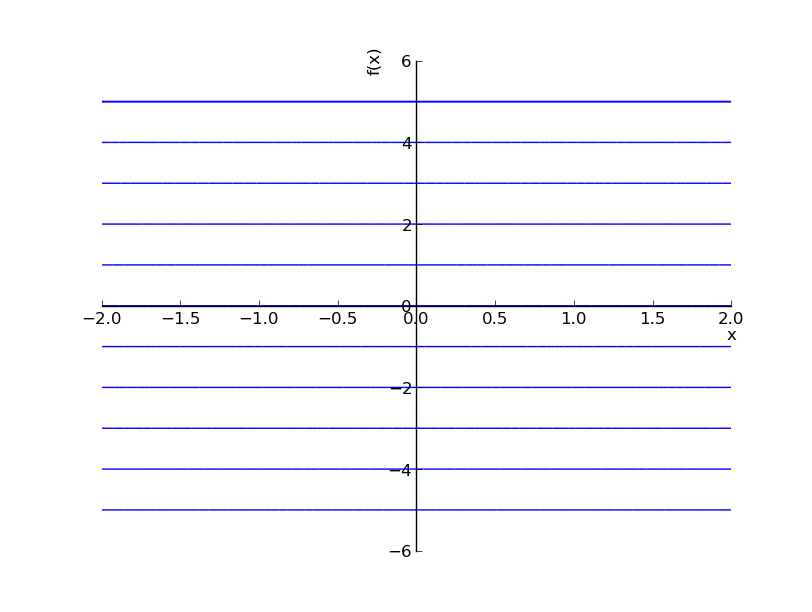
\includegraphics[scale=.3]{imagenes/sol_trivial.png}
 \end{wrapfigure}
La condición de simetría se reduce a 
\[
\frac{\frac{\partial\hat{y}}{\partial x}}{\frac{\partial\hat{x}}{\partial x}}=0
\]
Debemos tener que $\frac{\partial\hat{y}}{\partial x}=0$. Vale decir $\hat{y}$ es independiente de $x$. De allí la forma general de una simetría es 
\[\hat{x}=\hat{x}(x,y)\quad \hat{y}=\hat{y}(y).\]
\end{ejemplo}
 Hay muchas simetrías. Las traslaciones en cualquier dirección $(x,y)\mapsto (x+\alpha ,y+\beta)$ ($\alpha,\beta\in\rr$). Cambios de escala en ambos ejes  $(x,y)\mapsto (e^{\epsilon}x,y)$, $(x,y)\mapsto (x,e^{\epsilon}y)$. Reflexiones respecto ambos ejes  $(x,y)\mapsto (-x,y)$, $(x,y)\mapsto (x,-y)$.  Observar que el gráfico de las soluciones posee las mismas simetrías, pues en general \emph{las simetrías de una ecuación llevan soluciones en soluciones}.

 De todas las simetrías encontradas $\Gamma_{\epsilon}(x,y)=(e^{\epsilon}x,y)$, $\Gamma_{\epsilon}(x,y)=(x+\epsilon,y)$ y  $\Gamma_{\epsilon}(x,y)=(x+\epsilon,y)$ se llaman \emph{triviales} pues llevan una curva solución en si misma.  Cualquier cambio de la forma $\hat{x}=\hat{x}(x,y)\quad \hat{y}=y$ es trivial. \emph{Estamos interesados en hallar grupos de Lie uniparamétricos de simetrías no triviales.}




 \begin{ejemplo}{} Hallar simetrías de
\[\frac{dy}{dx}=f(x).\]
\end{ejemplo}
De acuerdo con \eqref{eq:subsder} se debe cumplir que
 \[\frac{\frac{\partial\hat{y}}{\partial x}+\frac{\partial\hat{y}}{\partial y}f(x)}{\frac{\partial\hat{x}}{\partial x}+\frac{\partial\hat{x}}{\partial y}f(x)}=f(\hat{x})\]
La forma de la ecuación sugiere el  \href{http://es.wikipedia.org/wiki/Ansatz}{ansatz}
   \[\boxed{\hat{x}=x},\quad \frac{\partial\hat{y}}{\partial x}=\frac{\partial\hat{x}}{\partial y}=0,\quad
   \frac{\partial\hat{y}}{\partial y}=\frac{\partial\hat{x}}{\partial x}. \]
 Luego 
\[\frac{\partial\hat{y}}{\partial y}=1\Rightarrow \boxed{\hat{y}=y+\epsilon} \]
con $\epsilon$ constante arbitraria. Hallamos que
\[\Gamma_{\epsilon}(x,y)=(x,y+\epsilon)\]
es un grupo de Lie uniparamétrico de simetrías. De manera similar
\[\Gamma_{\epsilon}(x,y)=(x+\epsilon,y)\]
es un grupo uniparamétrico de simetrías para 
\[\frac{dy}{dx}=f(y).\]
Geométricamente en el primer caso todas las soluciones se obtienen trasladando una cualquiera verticalmente y en el segundo caso horizontalmente.



\begin{tabular}{cc}
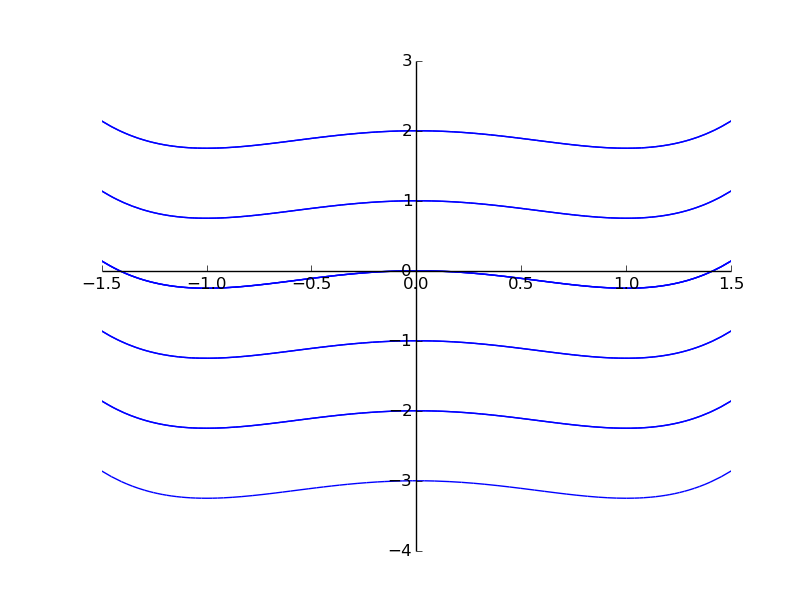
\includegraphics[scale=.3]{imagenes/sol_paralelas.png} &\hspace{-1.5cm}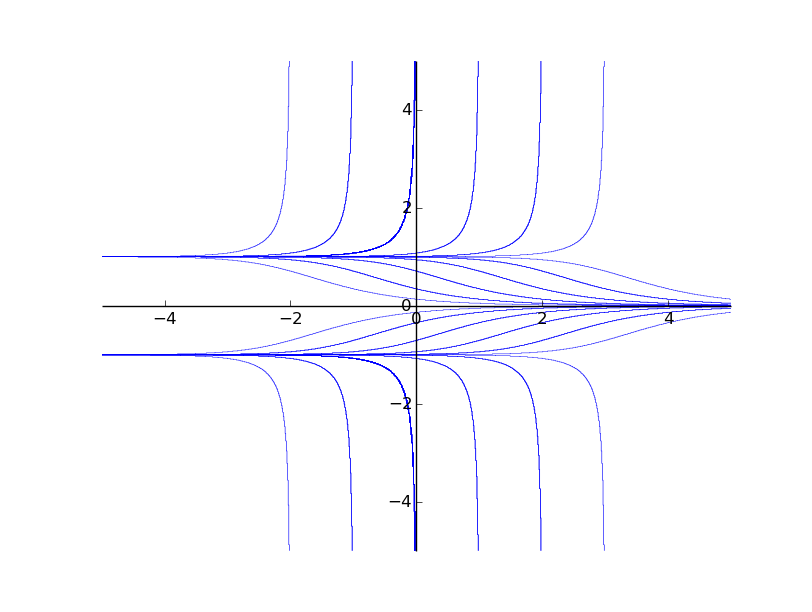
\includegraphics[scale=.3]{imagenes/sol_paralelas2.png} \\
Soluciones de $y'=x^3-x$ &\hspace{-1.5cm}Soluciones de $y'=y^3-y$
\end{tabular}





\begin{ejemplo}{}
 Demostrar que las rotaciones alrededor del origen es un grupo de Lie uniparamétrico de simetrías de
 \begin{equation}\label{eq:ejemplo_polar}
  \frac{dy}{dx}=\frac{y^3+x^2y-x-y}{x^3+xy^2-x+y}.
 \end{equation}
\end{ejemplo}
Sea $\Gamma_{\epsilon}$ la transformación que rota un ángulo $\epsilon$ alrededor del origen. Es un ejercicio demostrar que  $\{\Gamma_{\epsilon}|\epsilon\in\rr\}$ es un grupo uniparamétrico de simetrías. Se tiene la representación matricial
\[
\Gamma_{\epsilon}(x,y)= \begin{pmatrix} \hat{x}\\ \hat{y}
\end{pmatrix}=\begin{pmatrix} \cos(\epsilon) & -\sen(\epsilon)
\\ \sen(\epsilon) & \cos(\epsilon)
\end{pmatrix} \begin{pmatrix} x\\ y
\end{pmatrix}
\]

\[
\Gamma^{-1}_{\epsilon}(\hat{x},\hat{y})= \begin{pmatrix} x\\ y
\end{pmatrix}=\begin{pmatrix} \cos(\epsilon) & \sen(\epsilon)
\\ -sen(\epsilon) & \cos(\epsilon)
\end{pmatrix} \begin{pmatrix} \hat{x}\\ \hat{y}
\end{pmatrix}
\]


Para el cálculo recurrimos a \texttt{SymPy} (usamos \texttt{x\_n} en lugar de $\hat{x}$)

\begin{sympyblock}[][frame=single]
x,theta=symbols('x,theta')
y=Function('y')(x)
x_n=cos(theta)*x-sin(theta)*y
y_n=sin(theta)*x+cos(theta)*y
Expr2=y_n.diff(x)/x_n.diff(x)
Expr3=Expr2.subs(y.diff(),\
(y**3+x**2*y-x-y)/(x**3+x*y**2-x+y))
x_n,y_n=symbols('x_n,y_n')
Expr4=Expr3.subs([(y, -sin(theta)*x_n+cos(theta)*y_n),\
(x,cos(theta)*x_n+sin(theta)*y_n)])
Expr5=simplify(Expr4) 
\end{sympyblock}






\begin{wrapfigure}[15]{r}{5.5cm}
 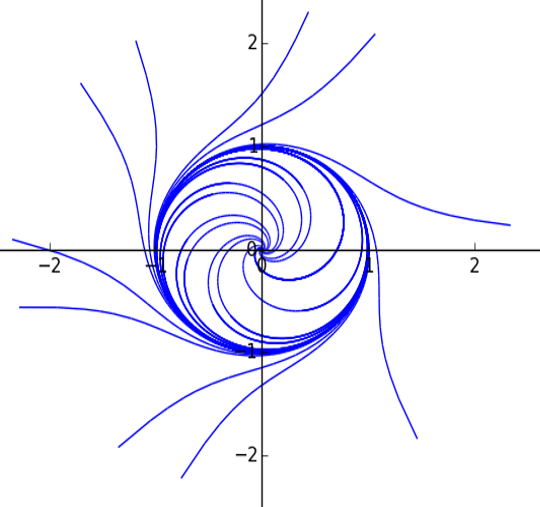
\includegraphics[scale=.4]{imagenes/sol_rotadas.png}
\end{wrapfigure}
La ecuación resultante es \emph{la misma}
\[\sympy{Expr5}\]
A la misma conclusión arribábamos si recordabamos que en en coordenadas polares la ecuación se escribe
\[\frac{dr}{d\theta}=r-r^3,\]
y que esta ecuación tiene las simetrías $\Gamma_{\epsilon}:(r,\theta)\mapsto (r,\theta+\epsilon)$. Si rotamos un ángulo fijo el gráfico de una solución obtenemos el gráfico de otra solución.








\begin{ejemplo}{ejem:tras} Supongamos que $y'=f(x,y)$ tiene  el grupo de Lie uniparamétrico de simetrías
\boxedeq{(\hat{x},\hat{y})=\Gamma_{\epsilon}(x,y)=(x,y+\epsilon)}{eq:tras_lie}
Usando la condición de simetrías \eqref{eq:cond_sim} tenemos
\[f(x,y)=f(\hat{x},\hat{y})=f(x,y+\epsilon).\]
La igualdad vale para todo $\epsilon$, luego poniendo $\epsilon=-y$ vemos que $f(x,y)=f(x,0):=f(x)$. Vale decir que $f$ es independiente de $y$ y la ecuación
\[y'=f(x),\]
se resuelve simplemente integrando.
\end{ejemplo}



\section{Órbitas, tangentes y curvas invariantes}


\begin{definicion}[Órbitas] Dado un grupo uniparamétrico de simetrías $G=\{\Gamma_{\epsilon}|\epsilon\in\rr\}$, y $(x_0,y_0)\in\rr^2$ llamamos \emph{órbita $(x_0,y_0)$ bajo la acción de  $G$} (simplemente órbita si es claro quien es $G$) a la curva
\[\{\Gamma_{\epsilon}(x_0,y_0)|\epsilon\in\rr\} \]
\end{definicion}

\begin{wrapfigure}[15]{r}{5.5cm}
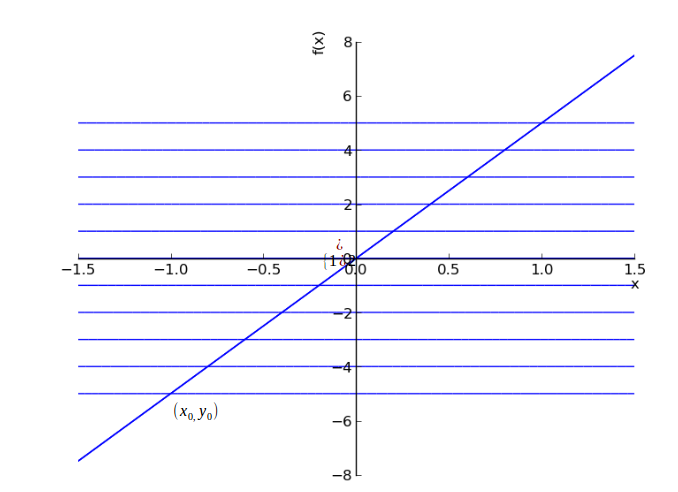
\includegraphics[scale=.3]{imagenes/sol_trivialB.png}
\end{wrapfigure}
Si $G$ es un grupo de simetrías no trivial, entonces es de esperar que la órbita de  $(x_0,y_0)$ cruce transversalmente las curvas solución. La órbita se usará como una nueva coordenada.
 La órbita atraves de $(x,y)$ es el conjunto de puntos de coordenadas
\begin{equation}\label{eq:orb} (\hat{x}(x,y,\epsilon),\hat{y}(x,y,\epsilon))=\Gamma_{\epsilon}(x,y),
\end{equation}
donde
\[(\hat{x}(x,y,0),\hat{y}(x,y,0))=(x,y).\]
Las ecuaciones \eqref{eq:orb} son ecuaciones parámetricas (parámetro $\epsilon$) de una  curva en el plano.

\begin{definicion}[Puntos invariantes]
Un punto $(x,y)$ se llama invariante si su órbita se reduce a $\{(x,y)\}$, vale decir
\[(x,y)=\Gamma_{\epsilon}(x,y),\quad\forall \epsilon>0\]
\end{definicion}






\begin{ejemplo}{} La órbita de $(x,y)$ bajo la acción del grupo  de Lie uniparamétrico
\[
\Gamma_{\epsilon}(x,y)= \begin{pmatrix} \hat{x}\\ \hat{y}
\end{pmatrix}=\begin{pmatrix} \cos(\epsilon) & -\sen(\epsilon)
\\ \sen(\epsilon) & \cos(\epsilon)
\end{pmatrix} \begin{pmatrix} x\\ y
\end{pmatrix}
\]
Son circunsferencias con centro en el origen. El punto $(0,0)$ es invariante.

\end{ejemplo}


\begin{definicion}[Campo vectorial de tangentes]
 Dado un grupo de Lie uniparamétrico $(\hat{x}(x,y,\epsilon),\hat{y}(x,y,\epsilon))=\Gamma_{\epsilon}(x,y)$  definimos el campo vectorial
\[(\xi(x,y),\eta(x, y))=\left(\left.\frac{d\hat{x}}{d\epsilon}\right|_{\epsilon=0}, \left.\frac{d\hat{y}}{d\epsilon}\right|_{\epsilon=0}   \right).\]
 $\xi$ y $\eta$ se llaman \emph{símbolos infinitesimales}.
 
 
Como $\hat{x},\hat{y}$ eran analíticas respecto a $\epsilon$ tenemos las fórmulas.

 
 \begin{equation}\label{eq:des_serie_infi}
\begin{array}{cc}
\hat{x}&=x+\epsilon\xi(x,y)+O(\epsilon^2)\\
\hat{y}&=y+\epsilon\eta(x,y)+O(\epsilon^2)\\
\end{array}
\end{equation}
 En un punto invariante \fbox{$\xi(x,y)=\eta(x,y)=0$}.
 
\end{definicion}





\begin{ejemplo}{}
Campo vectorial de infitesimales para las rotaciones. 
\end{ejemplo}
\begin{figure}[h]
 \begin{center}
  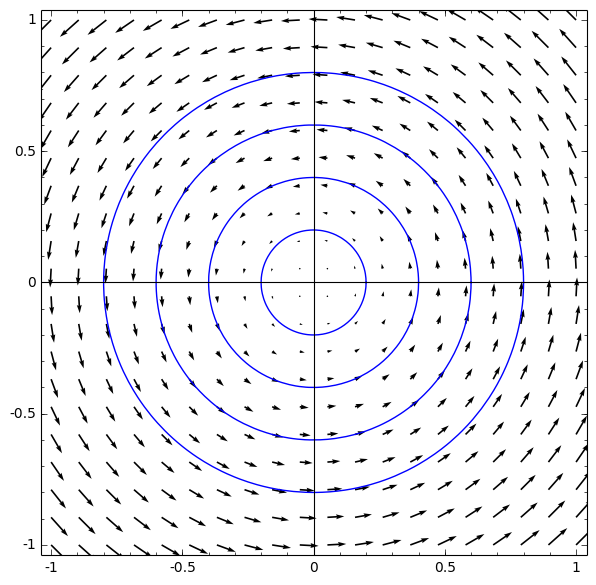
\includegraphics[scale=.3]{imagenes/CampoVectorial.png}
 \end{center}
\caption{Campo vectorial de infinitesimales $(\xi,\eta)$ }
\end{figure}

\begin{definicion}
 Más generalmente, un conjunto $C\subset\rr^2$ se dice \emph{invariante} por un grupo uniparamétrico de 
simetrías de Lie $\Gamma_{\epsilon}$ si y sólo si $\forall \epsilon: \Gamma_{\epsilon}(C)\subset C$, i.e. las órbitas de puntos en $C$ permanecen en $C$.
\end{definicion}

\noindent\textbf{Observaciones}
\begin{enumerate}
\item El conjunto unitario $\{(x,y)\}$ es invariante si y sólo si el punto $(x,y)$ 
es invariante.

\item Se $C$ es una curva plana suave, supongamos que $C$ viene dada por la ecuación implícita $g(x,y)=0$, con $\nabla g\neq 0$.  Supongamos que  $(\xi,\eta)\neq (0,0)$ sobre $C$. Entonces $C$ es invariante si y sólo si la tangente a  $C$ en cada punto $(x,y)$ es
paralela a $(\xi(x,y),\eta(x,y))$. La demostración de este hecho se propone como ejercicio.  
\item Si en particular $C$ es una curva que viene descripta como el gráfico de una función $y=h(x)$, entonces $C$ es invariante si y sólo si
\boxedeq{Q(x,y,y')=\eta(x,y)-h'\xi(x,y)\equiv 0.}{eq:inv}
En efecto, en este caso $g(x,y)=y-h(x)$ (notar que $\nabla g=(-h'(x),1)\neq 0$). Como $\nabla g$ es perpendicular a $C$ tenemos la ecuación \eqref{eq:inv}. La ecuación \eqref{eq:inv} se llama \emph{ecuación característica}.






\item Si además de lo anterior, $\Gamma_{\epsilon}$ es un grupo de Lie de simetrías de $y'=f(x,y)$ e $y(x)$ es una curva invariante y solución de la ecuación entonces:
\boxedeq{\overline{Q}(x,y)=\eta(x,y)-f(x,y)\xi(x,y)\equiv 0.}{eq:sol_inv}
A esta ecuación la llamamos  \emph{ecuación característica reducida}.

 \end{enumerate}


El recíproco también es cierto.
\begin{teorema}{teo:invariantes}
 Supongamos que $y(x)$ es solución de la ecuación característica y que
 \[\left.\frac{\partial \overline{Q}}{\partial y}\right|_{y=y(x)}\neq 0.\]
 Entonces $y(x)$ es una solución invariante de la ecuación.
\end{teorema}
\begin{proof} Será completada más adelante.
 
\end{proof}




\begin{ejemplo}{} La EDO
\begin{equation}\label{eq:eq_simple}y'=y
 \end{equation}
tiene simetrías de escala
\[(\hat{x},\hat{y})=\Gamma_{\epsilon}(x,y)=(x,e^{\epsilon}y).
 \]
Luego 
\[(\xi,\eta)=\left(\left.\frac{d\hat{x}}{d\epsilon}\right|_{\epsilon=0}, \left.\frac{d\hat{y}}{d\epsilon}\right|_{\epsilon=0}   \right)=(0,y)\]
Cualquier punto en el conjunto $\{(x,0)|x\in\rr\}$  es invariante. La ecuación característica reducida es.
\[\overline{Q}(x,y)=0\Rightarrow y=0\]
Esta formada enteramente por puntos invariantes.
\end{ejemplo}



\begin{ejemplo}{} Demostrar que la siguiente expresión es un grupo de Lie uniparamétrico de simetrías
\[(\hat{x},\hat{y})=\Gamma_{\epsilon}(x,y)=(e^{\epsilon}x,e^{(e^{\epsilon}-1)x}y),\]
para la ecuación \eqref{eq:eq_simple}.
Para este grupo tenemos
\[(\xi,\eta)=(x,xy)\]
Todo punto en $x=0$ es invariante. La ecuación característica reducida es
\[\overline{Q}(x,y)=0\Rightarrow xy-xy=0\]
De modo que estas simetrías actuan trivialmente sobre las soluciones. Llevan una solución en si misma. Chequeemos esta afirmación de manera directa. 
\end{ejemplo}

Buscamos el cambio de variables inverso
\[
\left.
\begin{array}{ll} 
  \hat{x}&= e^{\epsilon}x\\
  \hat{y}&=e^{(e^{\epsilon}-1)x}y\\
\end{array}
\right\} 
\Rightarrow  
    \left.
\begin{array}{ll} 
  x&= e^{-\epsilon}\hat{x}\\
  y&=e^{(e^{-\epsilon}-1)\hat{x}}\hat{y}\\
\end{array}
\right\} 
\]    

Las soluciones son $y=ke^x$, sustituímos en esta expresión, luego de unas operaciones, llegamos a $\hat{y}=ke^{\hat{x}}$.

\begin{ejemplo}{} La ecuación de Riccati
\[y'=xy^2-\frac{2y}{x}-\frac{1}{x^3},\quad x\neq 0\] 
 Tiene el grupo de Lie de simetrías
\[(\hat{x},\hat{y})=\Gamma_{\epsilon}(x,y)=(e^{\epsilon}x,e^{-2\epsilon}y).\]
Tenemos
\[(\xi,\eta)=(x,-2y).\]
La característica reducida
\[\overline{Q}(x,y)=\frac{1}{x^2}-x^2y^2=0.\]
Tenemos dos soluciones invariantes
\[y=\pm\frac{1}{x^2}.\] 

\end{ejemplo}

\section{Simetrías a partir de Infinitesimales }

 La mayoría de los métodos de simetría usan  $(\xi,\eta)$ en lugar de las simetrías en si mismas.
Por otra parte  $(\xi(\hat{x},\hat{y}),\eta(\hat{x},\hat{y}))$ determinan las simetrías a traves de las ecuaciones

\boxedeq{
\left\{
\begin{array}{ll}
\frac{d\hat{x}}{d\epsilon}&=\xi(\hat{x},\hat{y})\\
\frac{d\hat{y}}{d\epsilon}&=\eta(\hat{x},\hat{y})\\
\hat{x}(x,y,0)&=x\\
\hat{y}(x,y,0)&=y\\
\end{array}
\right.
}{eq:ecua_infinitesimales}
\textbf{Justificación de las ecuaciones.}
De la propiedad de grupo $ \Gamma_{\epsilon_1} \circ  \Gamma_{\epsilon}=
\Gamma_{\epsilon+\epsilon_1}$, deducimos 
\[\hat{x}(x,y,\epsilon+\epsilon_1)=\hat{x}(\hat{x}(x,y,\epsilon),
\hat{y}(x,y,\epsilon),\epsilon_1).\]
Derivando respecto a $\epsilon_1$ y evaluando en $\epsilon_1=0$ justificamos las EDO en 
\eqref{eq:ecua_infinitesimales}.




















El \emph{sistema de ecuaciones} \eqref{eq:ecua_infinitesimales}    puede ser difícil de resolver. Pero en algunos casos puede ser posible.

 \begin{ejemplo}{} Encontrar el grupo de simetrías para los infinitesimales $\xi(x,y),\eta(x,y))=(x^2,xy)$.
   \end{ejemplo}



\[ \frac{d\hat{x}}{d\epsilon}=\xi(\hat{x},\hat{y})=\hat{x}^2\text{ y }\hat{x}(x,y,0)=x
\Rightarrow \hat{x}=\frac{x}{1-\epsilon x}\]
y

\[ \frac{d\hat{y}}{d\epsilon}=\eta(\hat{x},\hat{y})=\hat{x}\hat{y}\text{ y }\hat{y}(x,y,0)=y
\Rightarrow \hat{y}=\frac{y}{1-\epsilon x}\]

\section{Condición de Simetría Linealizada}
En esta sección discutiremos una técnica para encontrar simetrías de ecuaciones. 


Desarrollando en serie de Taylor las funciones $\hat{x}$ e $\hat{y}$ en $\epsilon$ alrededror de $\epsilon=0$
\[
 \begin{split}
  \hat{x}&=x+\epsilon\xi+\mathcal{O}(\epsilon^2)\\
  \hat{y}&=y+\epsilon\eta+\mathcal{O}(\epsilon^2)
  \end{split}
\]
Reemplazando en la condición de simetría, que recordemos es
\[\frac{\frac{\partial\hat{y}}{\partial x}+\frac{\partial\hat{y}}{\partial y}
 f(x,y)}{\frac{\partial\hat{x}}{\partial x}+\frac{\partial\hat{x}}{\partial y}f(x,y)}
 =f(\hat{x},\hat{y}),
\] 
obtenemos
\[\frac{f+\epsilon\{\eta_x+f\eta_y\}+\mathcal{O}(\epsilon^2)}
{1+\epsilon\{\xi_x+f\xi_y\}+\mathcal{O}(\epsilon^2)}
=f(x+\epsilon\xi+\mathcal{O}(\epsilon^2),y+\epsilon\eta+\mathcal{O}(\epsilon^2))
\]



Desarrollando en serie de Taylor para $x$ e $y$ el segundo miembro y luego de algunas operaciones

\[f+\epsilon\{\eta_x+(\eta_y-\xi_x)f-\xi_yf^2\}+\mathcal{O}(\epsilon^2)=
 f+\epsilon\{\xi f_x+\eta f_y\}+\mathcal{O}(\epsilon^2)
\]
Cancelando $f$ dividiendo por $\epsilon$ y haciendo $\epsilon\to 0$ llegamos a la 
\emph{Condición de Simetría Linealizada}

\boxedeq{\eta_x+(\eta_y-\xi_x)f-\xi_yf^2=\xi f_x+\eta f_y}{eq:CondSimLin}

Recordando la característica reducida $\overline{Q}= \eta-f\xi$, la fórmula anterior se escribe más sintéticamente
\boxedeq{\overline{Q}_x+f\overline{Q}_y=f_y\overline{Q}}{eq:CondSimLin2}

Cada solución de \eqref{eq:CondSimLin2} conlleva una infinita cantidad de grupos de Lie de simetrías, porque si $\overline{Q}$ resueleve  \eqref{eq:CondSimLin2}  entonces para toda función $\xi$ el par $(\xi, \overline{Q}+f\xi)$ son infinitesimales para un grupo de Lie de simetrías de la ecuación. La solución trivial $\overline{Q}\equiv 0$ de  \eqref{eq:CondSimLin2}  se corresponde con simetrías triviales. En principio podríamos utilizar el método de características, que hemos visto en la unidad anterior, para resolver la ecuación lineal en derivadas parciales de primer orden \eqref{eq:CondSimLin2} que, recordando lo visto, se puede escribir
\[ \frac{dx}{1}=\frac{dy}{f}=\frac{d\overline{Q}}{f_y\overline{Q}}.\]
La primera igualdad en la ecuación anterior equivales a $dy/dx=f$, que es al fin y al cabo, la ecuación que queremos resolver. Así estas consideraciones parecen habernos llevado al origen de nuestro problema. No obstante, algunas veces es posible encontrar una solución de \eqref{eq:CondSimLin} recurriendo a un ansatz.

 \begin{ejemplo}{} Encontrar un grupo de Lie de simetrías no trivial de $y'=\frac{y}{x}+x$.
   \end{ejemplo}


 
 La condición de simetría linealizada es
 \[\eta_x+(\eta_y-\xi_x)\left(\frac{y}{x}+x\right)-\xi_y\left(\frac{y}{x}+x\right)^2
 =\xi \left(1-\frac{y}{x^2}\right)
+\frac{\eta}{x},\] 

que luce intimidante. Hagamos el ansatz $\xi=0$ y $\eta=\eta(x)$. Conseguimos
\[\eta_x-\frac{\eta}{x}=0\]
Cuya solucion general es $\boxed{\eta=cx}$. Ahora podemos encontrar simetrías de la ecuación. Recordando \eqref{eq:ecua_infinitesimales}, tenemos
\[
\left\{
\begin{array}{ll}
\frac{d\hat{x}}{d\epsilon}&=0\\
\frac{d\hat{y}}{d\epsilon}&=c\hat{x}\\
\hat{x}(x,y,0)&=x\\
\hat{y}(x,y,0)&=y\\
\end{array}
\right. 
\Rightarrow 
\left\{
\begin{array}{ll}
\hat{x}&=x\\
\hat{y}&=c\epsilon x+y\\
\end{array}
\right.
\]

Podemos constatar de manera directa que $\hat{x}=x$ e $\hat{y}=c\epsilon x+y$ constituyen un grupo de Lie uniparamétrico de simetrías de la ecuación, para el cual $\overline{Q}\neq 0$.


 \begin{ejemplo}{} Encontrar valiendose de SymPy los infinitesimales  de la ecuación \eqref{eq:ejemplo_polar}.
   \end{ejemplo}
   
\begin{sympyblock}[][frame=single]
from sympy import *
init_printing()
x,y=symbols('x,y',real=True)
f=(y**3+x**2*y-x-y)/(x**3+x*y**2-x+y)
\end{sympyblock}

Cómo en muchos otras situaciones que se presentan cuando intentamos resolver de manera exacta ecuaciones diferenciales,  debemos recurrrir a una heurística \marginpar{\textbf{Heurística:} ...significa «hallar, inventar» (etimología que comparte con eureka)... Cuando se usa como sustantivo, se refiere a la disciplina, el arte o la ciencia del descubrimiento... Cuando aparece como adjetivo, se refiere a cosas más concretas, como estrategias, reglas, silogismos y conclusiones heurísticas. Estos dos usos están íntimamente relacionados, ya que la heurística usualmente propone estrategias que guían el descubrimiento. El término fue utilizado por Albert Einstein en la publicación sobre efecto fotoeléctrico (1905). 
\begin{flushright}
 Wikipedia
\end{flushright}
 } con el objeto de resolver  el problema. Por ejemplo, SymPy incorpora una estrategia de busqueda entre distintos candidatos a infinitesimales, ver \cite{Lie_Sympy,cheb1997computer} para los detalles. Por ejemplo, la primer heurística que se enumera en \cite{Lie_Sympy} es la que usamos en el ejemplo anterior, es decir $\xi=0$ y $\eta=\eta(x)$. En el ejemplo actual, vamos a usar la siguiente heurística
 \[\xi=ax+by+h,\quad \eta=cx+dy+k.\]
\begin{sympyblock}[][frame=single]
a,b,c,d,h,k=symbols('a,b,c,d,h,k',real=True)
xi=a*x+b*y+h
eta=c*x+d*y+k
Q=eta-f*xi
\end{sympyblock}

Reemplazamos el valor de $Q$ en la condición de simetría linealizada.
\begin{sympyblock}[][frame=single]
CondSim=Q.diff(x)+f*Q.diff(y)-f.diff(y)*Q
CondSim=simplify(CondSim)
\end{sympyblock}
Llegamos a una ecuación de la forma
\[
 \frac{P_1(x,y)}{P_2(x,y)}=0,
\]
donde $P_1$ y $P_2$  son polinomios bivariados. Obviamente sólo nos interesa $P_1$, que podemos extraer de la siguiente forma 
\begin{sympyblock}[][frame=single]
P1,P2=fraction(CondSim)
P1
\end{sympyblock}
Obtenemos la siguiente expresión  monstruosa de $P_1$, que sólo reproducimos a modo anecdótico

\[
\begin{split}
P_1 =&- a x^{4} - 2 a x^{2} y^{2} - a x^{2} + 2 a x y - a y^{4} + a y^{2} - b x^{2} - 2 b x y\\
&+ b y^{2} - c x^{2} - 2 c x y+ c y^{2} - d x^{4} - 2 d x^{2} y^{2}
+ d x^{2} - 2 d x y\\
&- d y^{4} - d y^{2} + h x^{4} y - 2 h x^{3} + 2 h x^{2} y^{3} - 2 h x^{2} y - 2 h x y^{2} + h y^{5}\\
&- 2 h y^{3} + 2 h y - k x^{5} - 2 k x^{3} y^{2} + 2 k x^{3} - 2 k x^{2} y - k x y^{4} + 2 k x y^{2}\\
&- 2 k x - 2 k y^{3}
\end{split}
\]

Hay que resolver $P_1=0$. A pesar de la apariencia atemorizante de esta ecuación, es completamente inofensiva si tenemos en mente que el ``juego'' consiste en hallar los coeficientes $a,b,c,d,h,k$ que resuelven la ecuación para todo $x$ e $y$. De modo que podemos reemplazar $x$ e $y$ por distintos valores y resolver las ecuaciones resultantes. En el código debajo usamos el método \texttt{collect(x)} que agrupa los términos de una expresión que tienen la misma potencia para $x$.

\begin{sympyblock}[][frame=single]
P1.subs(y,0).collect(x)
\end{sympyblock}
Resulta
\[
 0=- k x^{5} - 2 k x + x^{4} (- a - d) + x^{3} (- 2 h + 2 k) + x^{2} (- a - b - c + d)
\]
Es un polinomio en $x$ que debería ser identicamente $0$, debe para ello tener todos los coeficientes iguales a $0$. Inferimos  inmediatamente de esto que $k=h=0$, $d=-a$ y $c=-2a-b$. Reemplacemos ahora $y$ por $1$.  

\begin{sympyblock}[][frame=single]
P11=P1.subs({h:0,k:0,d:-a,c:-2*a-b})
P11.subs(y,1).collect(x)
\end{sympyblock}
Resulta en la expresión $8ax$,  que si es identicamente $0$ fuerza  que $a=0$. Luego $d=0$ y $c=-b$. El valor de $c$ es arbitrario, se puede elegir cualquiera, elejimos $c=1$ y por consiguiente $b=-1$.   
 
 \begin{sympyblock}[][frame=single]
xi=xi.subs({d:0,a:0,b:-1,c:1,h:0,k:0})
eta=eta.subs({d:0,a:0,b:-1,c:1,h:0,k:0})
xi,eta
\end{sympyblock}
Cocnluímos $\xi=-y$ y $\eta=x$. Todavía no estamos seguros que estos $\xi$ y $\eta$ resuelvan nuestro problema. El razonamiento anterior está incompleto sino chequeamos que la solución obtenida resuelve la ecuación de simetría linealizada para todo $x$ e $y$, esto porque con la metodología  utilizada solo estamos seguros que los valores obtenidos para los coeficientes   solucionan el problema en los valores que elegimos para $y$ ($y=0$ e $y=1$). Ahora podemos chequear que en realidad se resuelve la ecuación de simetría linealizada para cualquier valor de $x$ e $y$.  
 \begin{sympyblock}[][frame=single]
CondSimLin=Q.diff(x)+f*Q.diff(y)-f.diff(y)*Q
CondSimLin.simplify()
\end{sympyblock}


Que definitivamente establece que la elección que hemos hecho resuelve el problema.

 
\textbf{Completación de la demostración  del Teorema \ref{teo:invariantes}}.
Restaba demostrar que si $y(x)$ resuelve la ecuación $\overline{Q}(x,y(x))=0$ y $\overline{Q}_y\neq 0$ en los puntos a lo largo de la curva $(x,y(x))$ entonces $y(x)$ es solución invariante de la ecuación $y'=f$. 

Por el Teorema de la función implícita,
la condición de simetría linealizada \eqref{eq:CondSimLin2} y $\overline{Q}=0$
\[y'(x)=-\frac{\overline{Q}_x}{\overline{Q}_y}=f-f_y\frac{\overline{Q}}{\overline{Q}_y}=f\]
Luego $y$ es solución de la ecuación. El hecho de que es invariante es simplemente la igualdad 
$\overline{Q}=0$.









\section{Coordenadas canónicas}

\subsection{Definición y ejemplos}
\begin{definicion}[Coordenadas canónicas]   Diremos que las coordenadas $(r,s)$ son canónicas respecto a el grupo de Lie de simetrías $\Gamma_{\epsilon}$  si en las coordenadas $(r,s)$ la acción de grupo es la traslación

\boxedeq{(\hat{r},\hat{s}):= (r(\hat{x},\hat{y}),s(\hat{x},\hat{y}))=(r(x,y),s(x,y)+\epsilon).}{eq:coorcan}
\end{definicion}
 \begin{ejemplo}{} Las coordenadas polares son canónicas respecto al grupo de Lie de rotaciones. Las rotaciones en coordenadas cartesianas y polares se escriben
\[
 \begin{pmatrix} \hat{x}\\ \hat{y}
\end{pmatrix}=\begin{pmatrix} \cos(\epsilon) & -\sen(\epsilon)
\\ \sen(\epsilon) & \cos(\epsilon)
\end{pmatrix} \begin{pmatrix} x\\ y
\end{pmatrix},\quad \begin{array}{ll} \hat{r}&=r\\ \hat{\theta}&=\theta+\epsilon\\ 
\end{array}
\]
\end{ejemplo}

Derivando las ecuaciones \eqref{eq:coorcan} respecto a $\epsilon$ obtenemos
\boxedeq{
\begin{array}{ll}
\xi(x,y)\frac{\partial r}{\partial x}+\eta(x,y)\frac{\partial r}{\partial y}&=0\\
\xi(x,y)\frac{\partial s}{\partial x}+\eta(x,y)\frac{\partial s}{\partial y}&=1
\end{array}
}{eq:coor_can_dif}
 Los cambios de coordenadas deben ser invertibles, de modo que pediremos la condición de no degeneración
\boxedeq{\frac{\partial r}{\partial x}\frac{\partial s}{\partial y}-\frac{\partial r}{\partial y}\frac{\partial s}{\partial x}\neq 0}{eq:no_deg}





\noindent\textbf{Observaciones:}
\begin{enumerate}
\item El vector tangente en cualquier punto no invariante es paralelo a la curva $r=\hbox{cte}$ que pasa por ese punto. Luego esa curva continene las órbitas de cada punto en ella. Las órbitas son invariantes, así  $r$ se llama la \emph{coordenada invariante}. Las curvas $s=\hbox{cte}$ son transversales a las órbitas.
\item Las coordenadas canónicas no estan definidas en un punto $(x,y)$ invariante pues en esos puntos $\xi(x,y)=\eta(x,y)=0$.

\item Las coordenadas canónicas estan definidas en un entorno de cualquier   punto no invariante. Esta afirmación requiere una demostración que utiliza métodos y conceptos que estan fuera de los objetivos de este curso.

\item Las coordenadas canónicas no son únicas. De hecho si $(r,s)$ son canónicas $(\tilde{r},\tilde{s})=(F(r),G(r)+s)$ lo son para cualquier $F$ y $G$ con $F'(r)\neq 0$ (para la no degeneración).

\end{enumerate}






\section{Encontrando coordenadas canónicas}

 \subsection{Integrales primeras}
\begin{definicion}[Integrales primera] Una integral primera de la EDO $y'=f(x,y)$ es una función $\phi(x,y)$ que es constante a lo largo de cualquier curva solución de la EDO. Se la denomina también \emph{magnitud conservada}.
 \end{definicion}



 \begin{teorema}[Propiedad de conservación de coordenadas canónicas]{} Si $(r,s)$ son coordenadas canónicas de una grupo de Lie de simetrías entonces $r$ es una integral primera de la ecuación
\begin{equation}\label{eq:int_pri} \frac{dy}{dx}=\frac{\eta(x,y)}{\xi(x,y)}.
\end{equation}
\end{teorema}
\textbf{Dem.} La afirmación del teorema es consecuencia de que el campo $(\xi,\eta)$ es tangente a las curvas $r=c$, con $c$ constante. Justifiquemos el teorema del siguiente modo.  Supongamos $y(x)$ solución de la EDO, es suficiente demostrar que $\frac{d}{dx}r(x,y(x))=0$. Pero, en efecto
\[
\begin{array}{lll}
 \frac{d}{dx}r(x,y(x)) &=\frac{\partial r}{\partial x}+\frac{\partial s}{\partial y}y' &\text{(regla cadena)}\\
&=\frac{\partial r}{\partial x}+\frac{\partial s}{\partial y}\frac{\eta(x,y)}{\xi(x,y)}& \text{(Ec. \eqref{eq:int_pri})}\\
&=0 & \text{(Ec. \eqref{eq:coor_can_dif})}\\
\end{array}
\]
\qed

\begin{ejemplo}{} Ya conocemos las coordenadas canónicas de las rotaciones,
 \[
 \begin{pmatrix} \hat{x}\\ \hat{y}
\end{pmatrix}=\begin{pmatrix} \cos(\epsilon) & -\sen(\epsilon)
\\ \sen(\epsilon) & \cos(\epsilon)
\end{pmatrix} \begin{pmatrix} x\\ y
\end{pmatrix}\Rightarrow  \begin{pmatrix} \xi\\ \eta
\end{pmatrix}= \begin{pmatrix} -y\\ x
\end{pmatrix}
\]
hallemosla por el método propuesto.
\end{ejemplo}
Hay que resolver
\[\frac{dy}{dx}=-\frac{x}{y}\Rightarrow ydy=-xdx\Rightarrow y^2+x^2=C\]
Luego $r=\sqrt{x^2+y^2}$ es una integral primera. 



La coordenada $r$ es constante sobre los puntos en la gráfica de una solución de \eqref{eq:int_pri}. Sobre esos puntos $(x,y(x))$, la coordenada $s$ satisface:

\begin{equation} \label{eq:coor_can_s}
\begin{array}{lll}
\frac{ds}{dx}&=\frac{\partial s}{\partial x}+\frac{\partial s}{\partial y} y'(x) & \hbox{(Regla cadena)}\\
&=\frac{\partial s}{\partial x}+\frac{\partial s}{\partial y} \frac{\eta}{\xi} &
  \eqref{eq:int_pri}\\
&=\frac{1}{\xi} &\hbox{\eqref{eq:coor_can_dif}}.
\end{array}
\end{equation}
Ahora podemos aprovechar que ya conocemos $r$ y  expresar $y$ como función de $r,x$. Luego

\begin{teorema}[Expresión para $s$]{}
\boxedeq{s=\int\frac{ds}{dx}dx=\int\frac{dx}{\xi(x,y(r,x))}.}{eq:expr_coor_s}
\end{teorema}
 

En la igualdad resultante  reemplazamos $r$ por su expresión en las variables $x,y$.


Si ocurriese que $\xi=0$ y $\eta\neq 0$. Entonces por \eqref{eq:int_pri} $r_y=0$, de modo que $r$ es sólo función de $x$. Se puede asumir $r=x$. Además $\eta s_y=1$, entonces
\boxedeq{s=\int\frac{dy}{\eta(r,y)} .}{eq:s_xi_0}


\begin{ejemplo}{} Retornando al ejemplo de las rotaciones, donde hallamos que $r=\sqrt(x^2+y^2)$, vemos que
\[s=\int\frac{dx}{-y}=-\int\frac{dx}{\sqrt{r^2-x^2}}=\arccos\left(\frac{x}{r}\right).\]
Por consiguiente  $s$ es el ángulo polar.
\end{ejemplo}


\label{pag_ejem_canon1}
\begin{ejemplo}{} Encontrar coordenadas canónicas para el grupo de Lie de simetrías
\[(\hat{x},\hat{y})=(e^{\epsilon}x,e^{k\epsilon}y)\quad k>0.\]
\end{ejemplo}
El vector tangente es
\[(\xi,\eta)=\left(\left.\frac{d\hat{x}}{d\epsilon}\right|_{\epsilon=0},\left.\frac{d\hat{y}}{d\epsilon}\right|_{\epsilon=0}\right)=(x,ky).\]
Resolvamos la ecuación  \eqref{eq:int_pri} 
\[\frac{dy}{dx}=\frac{ky}{x}\Rightarrow y=Cx^k.\]
Luego $\Phi=y/x^k$ es integral primera. Entonces podemos tomar $r=y/x^k$.  Para $s$
\label{pag_ejem_canon2}
\[s=\int\frac{dx}{\xi}=\frac{dx}{x}=\ln|x|.\]
Entonces $(r,s)=(yx^{-k},\ln|x|)$ son coordenadas canónicas. No estan definidas en $x=0$.
Podemos encontrar coordenadas canónicas definidas en $x=0$ del siguiente modo. Recordamos que para todas $F$ y $G$
\[(\tilde{r},\tilde{s})=(F(r),G(r)+s)=(F(x^{-k}y),G(x^{-k}y)+\ln|x|).\]
Son canónicas también. Si tomamos $F(r)=1/r$ y $G(r)=\frac{1}{k}\ln|r|$, evitamos la singularidad. Luego

\[(\tilde{r},\tilde{s})=(x^ky^{-1},\frac{1}{k}\ln|y|).\]
Son canónicas, están definidas en $x=0$ pero no en $y=0$.  

%%%%%%%%%%%%%

\begin{ejemplo}{} Encontrar coordenadas canónicas para
\[(\hat{x},\hat{y})=\left( \frac{x}{1-\epsilon x},\frac{y}{1-\epsilon x}\right).\]
\end{ejemplo}

\[(\xi,\eta)=\left(\left.\frac{d\hat{x}}{d\epsilon}\right|_{\epsilon=0},\left.\frac{d\hat{y}}{d\epsilon}\right|_{\epsilon=0}\right)=(x^2,xy).\]
\label{pag:can_ejem_p}
\[\frac{dy}{dx}=\frac{\eta}{\xi}=\frac{y}{x}\Rightarrow \frac{y}{x}=\hbox{cte}.\]

Podemos tomar $r=y/x$. Para $s$
\[s=\int\frac{dx}{x^2}=-\frac{1}{x}.\]
Luego $(r,s)=(\frac{y}{x},-\frac{1}{x})$ son canónicas.

En este caso los puntos sobre $x=0$ son invariantes, no podemos definir coordenadas canónicas allí.

Lo podemos desarrollar con \texttt{SymPy}. 

\begin{sympyblock}[][frame=single]
x,y,epsilon=symbols('x,y,epsilon')
T=Matrix([x/(1-epsilon*x),y/(1-epsilon*x)])
xi=T[0].diff(epsilon).subs(epsilon,0)
print(xi)
eta=T[1].diff(epsilon).subs(epsilon,0)
print(eta/xi)
y=Function('z')(x)
sol=dsolve(y.diff(x)-y/x,y)
print(sol)
Integral(1/xi,x).doit()
\end{sympyblock}





\subsection{Infinitesimales$\to$Simetrías (Revisitado)}
Las coordenadas canónicas nos dan otra manera de encontrar simetrías a partir de los infinitesimales siguiendo el procedimiento:

\begin{enumerate}
\item Determinar las coordenadas canónicas  (sólo necesitamos conocer los infinitesimales).
\item Expresamos las relaciones $\hat{r}=r$ y $\hat{s}=s+\epsilon$ en las coordenadas $x,y$.
\end{enumerate}


\begin{ejemplo}{} Hallar el grupo de simetrías asociado a los infinitesimales 
$\xi=x^2$ y $\eta=xy$.
\end{ejemplo}


\begin{enumerate}
\item En la sección \ref{pag:can_ejem_p} hallamos las coordenadas canónicas $(r,s)=\left(\frac{y}{x},-\frac{1}{x}\right)$ asociadas a los infinitesimales dados.
\item Entonces
\[\begin{split}
(\hat{r},\hat{s})&=(r,s+\epsilon)\Rightarrow \frac{\hat{y}}{\hat{x}}=\frac{y}{x}\text{ , }-\frac{1}{\hat{x}}=-\frac{1}{x}+\epsilon\\
&\Rightarrow \hat{x}=\frac{x}{1-\epsilon x} \text{ , } \hat{y}=\frac{y}{1-\epsilon x}.
\end{split}
\] 
\end{enumerate}



\section{Resolviendo EDO con grupos de Lie de simetrías}
\subsection{Método de solución}
Finalmente, toda la teoría expuesta nos permite elaborar un método que puede resolver una ecuación dada supuesto que conocemos un grupo de Lie de simetrías de ella.  Supongamos dado  un grupo de Lie de simetrías $(\hat{x},\hat{y})$ de la ecuación
\boxedeq{y'=f(x,y)}{eq:eq_princi}
 Supongamos  que las simetrías son no triviales. Según \eqref{eq:sol_inv} debemos tener
 \[\eta(x,y)\not\equiv f(x,y)\xi(x,y)\]
La razón de esta condición es que si fuese falsa entonces la ecuación \eqref{eq:int_pri} es la misma que la ecuación \eqref{eq:eq_princi} y el método es inútil.

Supongamos $(r,s)$ coordenadas canónicas. La ecuación en las coordenadas $(r,s)$, según \eqref{eq:subsder}, se escribirá
\boxedeq{\frac{ds}{dr}=\hat{f}(r,s):=\frac{s_x+f(x,y)s_y}{r_x+f(x,y)r_y}.}{eq:prin_en_canon}

Las coordenadas canónicas se definen por \eqref{eq:coorcan} de modo que el grupo de simetrías actúe por traslación $(\hat{r},\hat{s})=(r,s+\epsilon)$.
Cómo se justifica en el Ejemplo  \ref{ejem:tras}, $\hat{f}$ es independiente de $s$, por consiguiente la ecuación se reduce a
\boxedeq{\frac{ds}{dr}=\hat{f}(r)}{eq:ecu_prin_canonica}
que se resuelve integrando.


\begin{ejemplo}{} Resolver
\[y'=xy^2-\frac{2y}{x}-\frac{1}{x^3},\quad x\neq 0,\]
sabiendo que la ecuación es invariante para el grupo de simetrías
\[(\hat{x},\hat{y})=(e^{\epsilon}x,e^{-2\epsilon}y).\]
\end{ejemplo}
Por los resultados de la sección \ref{pag_ejem_canon1}:
\[(r,s)=(x^2y,\ln|x|)\]
son canónicas. Según \eqref{eq:prin_en_canon} la ecuación en $(r,s)$ es:
\[\frac{dr}{ds}=\frac{\frac{1}{x}}{2xy+x^2\left(  xy^2-\frac{2y}{x}-\frac{1}{x^3}     \right)}=\frac{1}{x^4y^2-1}=\frac{1}{r^2-1}\]
\begin{wrapfigure}[15]{r}{7cm}
\begin{center}
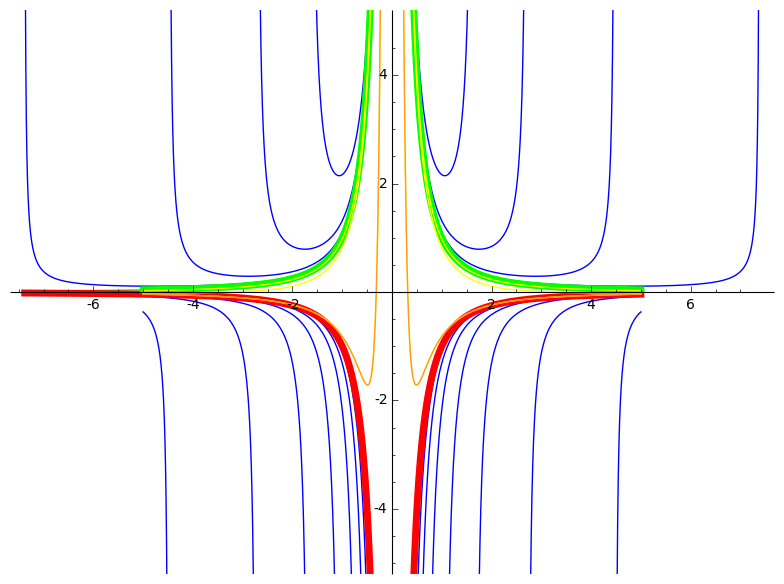
\includegraphics[scale=.3]{imagenes/SolGrup.png}
\caption{Soluciones de  $y'=xy^2-\frac{2y}{x}-\frac{1}{x^3}$}\label{fig:sol_met_lie}
\end{center}
\end{wrapfigure}
Como sabíamos que debía suceder el resultado del segundo miembro no depende sólo de $r$. Integrando
\[s=\frac12\ln\left( \frac{r-1}{r+1}  \right)+C.\]
Sustituyendo
\[\ln|x|=\frac12\ln\left( \frac{x^2y-1}{x^2y+1}  \right)+C.\]
Despejando
\begin{equation}\label{eq:sol_ejem}y =-\frac{x^2 + C}{x^2(x^2 - C)}\end{equation}
La ecuación característica reducida \eqref{eq:sol_inv} es para la ecuación de este ejemplo:
\[0=\overline{Q}=-2y- \left(xy^2-\frac{2y}{x}-\frac{1}{x^3}  \right)x=-x^2y^2+\frac{1}{x^2}\]
Cuyas soluciones son
\[y=\pm\frac{1}{x^2}.\]
Que además son solución de la ecuación diferencial. La curva $y=-1/x^2$ se obtiene de \eqref{eq:sol_ejem} con $C=0$. La  curva $y=-1/x^2$. En la figura \ref{fig:sol_met_lie} graficamos las distintas soluciones.Las curvas azules y naranjas se corresponden con las gráficas de \eqref{eq:sol_ejem} con $c>0$ y $c<0$ respectivamente. La verde es la de $y=1/x^2$ y la roja de $y=-1/x^2$.









\begin{ejemplo}{} Resolver
\[y'=\frac{y+1}{x}+\frac{y^2}{x^3},\quad x\neq 0,\]
sabiendo que la ecuación es invariante para el grupo de simetrías
\[(\hat{x},\hat{y})=\left(\frac{x}{1-\epsilon x},\frac{y}{1-\epsilon x}   \right).\]
\end{ejemplo}
Ya hemos computado las coordenadas canónicas en la subsección \ref{pag:can_ejem_p}:
\[(r,s)=\left(\frac{y}{x},\frac{1}{x}\right).\]
Por \eqref{eq:prin_en_canon} la ecuación se escribe
\[\frac{dr}{ds}=\frac{-\frac{1}{x^2} }{-\frac{y}{x^2}+\frac{1}{x}\left(
\frac{y+1}{x}+\frac{y^2}{x^3}\right)}=\frac{1}{1+r^2},\]
cuya solución es
\[s=\arctan(r)+C\Rightarrow y=-x\tan\left(\frac{1}{x}+C\right).\]



\subsection{Ecuaciones homogéneas}
\begin{ejemplo}{} En este ejemplo deduciremos nuevamente el método de solución de ecuaciones homogéneas apelando a las simetrías. Es decir, queremos resolver la ecuación
\boxedeq{y'=F\left(\frac{y}{x}\right).}{eq:homogenea}
\end{ejemplo}
Aquí tenemos el Grupo de Lie de simetrías de cambio de escalas
\[(\hat{x},\hat{y})=(e^{\epsilon}x,e^{\epsilon}y).\] 
Por los resultados de la subsección \ref{pag_ejem_canon1}, $(r,s)=(y/x,\ln|x|)$ son canónicas y la ecuación se escribe
\[\frac{ds}{dr}=\frac{\frac{1}{x}}{-\frac{y}{x^2}+\frac{F\left(\frac{y}{x}\right)}{x}}=\frac{1}{F(r)-r}.\]
La solución general es 
\[\ln|x|=\int^{y/x}\frac{dr}{F(r)-r}+c.\]




\subsection{Método de Lie y \texttt{SymPy}}
\text{SymPy} Incorpora distintas estrategías para resolver ecuaciones por el método de Lie. Hay mucho por indagar al respecto, pero sólo vamos a mencionar una función para calcular los infinitesimales $(\xi,\eta)$.  Aprovechamos para mostrar como luce una consola de \texttt{ipython}, otra manera de usar \texttt{Python} y \texttt{SymPy}.

\begin{sympyblock}[][frame=single]
x=symbols('x')
y=Function('y')(x)
from sympy.solvers.ode import infinitesimals
xi_eta=infinitesimals((y+1)/x+y**2/x**3-y.diff(x))
 
\end{sympyblock}

\[\sympy{xi_eta}\]



\section{Diagrama conceptual}

\begin{center}
 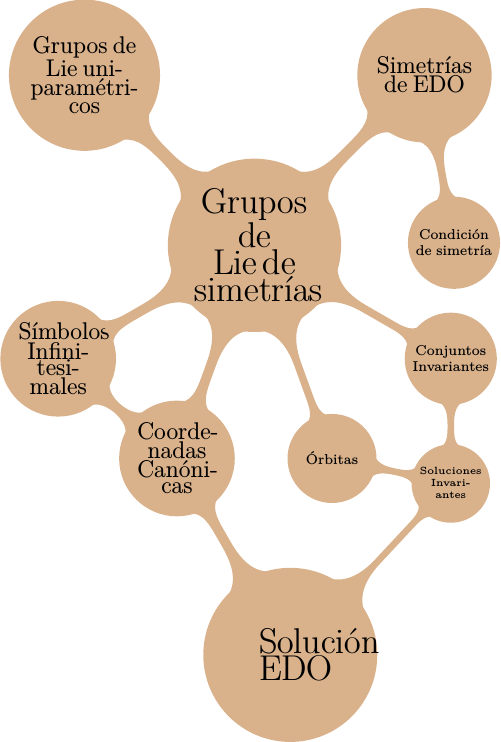
\includegraphics[scale=.5]{imagenes/diagrama.png}
\end{center}


\begin{subappendices}
 

\section{Formas Diferenciales, una introducción ingenua}%\label{section:fromas}





 La  expresión \eqref{eq:gral_orden1} es más asimétrica, entre las variables $x$ e $y$ una de ellas es independiente ($x$) y la otra independiente  ($y$).  La expresión \eqref{eq:gral_orden1_FormDif}  es  más simétrica, las dos variables tienen el mismo estatus.

 Las expresiones del tipo \eqref{eq:gral_orden1_FormDif} representan un ente matemático importante llamado \href{http://es.wikipedia.org/wiki/Forma_diferencial}{forma diferencial} . No disponemos del tiempo necesario para dotar con entidad matemática el concepto de forma diferencial. Tampoco  resulta de vital importancia. Pero las reglas que rigen la combinación de las formas diferenciales son muy simples y nos gustaría describir este aspecto de las formas diferenciales brevemente; como motivación para un estudio posterior más profundo y para que el lector gane en confianza en su manipulación. Daremos así una pintura de las formas diferenciales incompleta, por cuanto sólo diremos como ellas se combinan pero no contestaremos la pregunta de que son. Sólo digamos, para advertir al lector sobre los requisítos teóricos que se requieren, que las formas diferenciales se encuentran asociados al concepto de variedad diferencial, concepto este que generaliza al de curva y superficie.  Más 
concretamente, las formas diferenciales son funciones que toman valores en los duales de los espacios tangentes a las variedades diferenciales. En particular hay formas diferenciales asociadas a los espacios euclideo, que podemos identificar con  $\rr^n$.

Aqui vamos a pensar a las formas diferenciales como objetos puramente formales sobre los que actúa un operador $d$, leyes de composición internas y externas. Se construyen formas diferenciales invocando un sistema de coordenadas $x_1,\ldots,x_n$. Estas coordenadas, deben ser coordenadas de alguna variedad diferencial, pero, por simplicidad, supondremos que son coordenadas cartesianas ortogonales de un espacio euclideo. Las formas diferenciales forman un espacio vectorial con una operación de suma $+$ y producto por un escalar. Además tienen definido un producto $\wedge$, llamado \href{https://es.wikipedia.org/wiki/Producto_exterior}{producto exterior} , que posee  algunas particularidades.  Como los polinomios, las formas diferenciales tienen grado. Por eso se dice que forman un álgebra graduada. A diferencia de los polinomios, este grado no supera la dimensión $n$ del espacio ($\rr^n$ o más generalmente una variedad) a la que están asociadas. Para ser más exactas, la única forma 
de 
grado $k>n$ es la trivial, esto es la nula. Denotamos $\Lambda_k$ las formas de grado $k$, siendo $\Lambda =\bigoplus_{k=0}^{n}\Lambda_k$ el espacio vectorial de todas ellas. Luego $d:\Lambda\to\Lambda$ y $\wedge:\Lambda\times\Lambda\to \Lambda$. Ahora describimos unas simples reglas de las formas,  $d$ y $\wedge$.



\begin{enumerate}
   \item Una 0-forma diferencial es una función $g(x_1,\ldots,x_n)$.

  \item Si $\alpha\in\Lambda_k$ y $\beta\in\Lambda_p$ entonces $\alpha \wedge \beta\in \Lambda_{k+p}$.
  \item El producto $\wedge$ es asociativo, distributivo y satisface una especia de anticonmutatividad, especídficamente si $\alpha\in\Lambda_k$ y $\beta\in\Lambda_p$ entonces $\alpha\wedge \beta=(-1)^{kp}\beta\wedge\alpha$. En particular $\alpha\wedge\alpha=0$ cuando $\alpha$ es un $k$-forma con $k$ impar.
  \item El diferencial satisface
  \begin{enumerate}
    \item Si $\omega$ es una $k$-forma diferencial $d\omega$ es una $k+1$ forma diferencial.
    \item  $d^2\omega=d(d\omega)=0$, para toda $\omega\in\Lambda$.
    \item Si $\alpha\in\Lambda_k$ entonces  $d(\alpha\wedge\beta)=d\alpha\wedge\beta+(-1)^k\alpha\wedge d\beta$.
    \item En el caso de $0$-forma (función) $g(x_1,\ldots,x_n)$ el diferencial se define
    \[dg=\frac{\partial g}{\partial x_1}dx_1+\cdots+\frac{\partial g}{\partial x_n}dx_n\]

  \end{enumerate}
  \item Las expresiones $dx_i$, $i=1,\ldots,n$ forman una especie de base del espacio de las formas $\Lambda$, en el sentido que cualquier $k$ forma $\alpha$ se expresa de la siguiente manera:
  \[\alpha=\sum_{1\leq i_1<\cdots i_k\leq n}g_{i_1\ldots i_k} dx_{i_1}\wedge\cdots\wedge dx_{i_n},\]
  para ciertas funciones $g_{i_1\ldots i_k}$. Observar que la suma se extiende sobre todos los subconjuntos ordenados de $\{1,\ldots,n\}$.
\end{enumerate}


Una $k$-forma diferencial $\alpha$ se llama \href{https://es.wikipedia.org/wiki/Formas_diferenciales_cerradas_y_exactas}{exacta}  cuando es el diferencial de una $k-1$-forma y se dice \href{https://es.wikipedia.org/wiki/Formas_diferenciales_cerradas_y_exactas}{cerrada}  cuando $d\alpha=0$. Las propiedades de las formas implican que toda forma exacta es cerrda. Un famoso \href{https://es.wikipedia.org/wiki/Formas_diferenciales_cerradas_y_exactas#Lema_de_Poincar.C3.A9}{Lema de Poincare}  trata con el recíproco de esta afirmación.

Las reglas anteriores permiten computar cualquiera de las operaciones.
\begin{ejemplo}{} Si $\alpha=M(x,y)dx+N(x,y)dy$ es una 1-forma de $\rr^2$, entonces
\[ \begin{split}
    d\alpha&=dM\wedge dx-Md^2x + dN\wedge dy-Nd^2y\\
    &=\left(\frac{\partial M}{\partial x}dx+ \frac{\partial M}{\partial y}dy\right)\wedge dx+
    \left(\frac{\partial N}{\partial x}dx+ \frac{\partial N}{\partial y}dy\right)\wedge dy\\
    &= \left(\frac{\partial N}{\partial x}- \frac{\partial M}{\partial y}\right) dx\wedge dy
   \end{split}
\]
Recordemos el famoso \href{https://es.wikipedia.org/wiki/Teorema_de_Green}{Teorema de Green} , que afirmaba que si $D\subset \rr^2$ era una región cuyo borde $C=\partial D$ era una curva cerrada simple, entonces
\[\ointctrclockwise_{\partial D} Mdx +Ndy=\iint_D \left(\frac{\partial N}{\partial x}- \frac{\partial M}{\partial y}\right) dx dy.\]
Utilizando formas diferenciales este resultado se escribe de la manera, mucho más compacta y sugerente
\[\ointctrclockwise_{\partial D} \alpha = \iint_Dd\alpha,\]
donde $\alpha =M(x,y)dx+N(x,y)dy$.  Esto es una relación clave de las formas diferenciales que se generaliza en un teorema fundamental de la matemática llamado \href{https://es.wikipedia.org/wiki/Teorema_de_Stokes}{Teorema de Stokes} .
\end{ejemplo}




\begin{ejemplo}{} Computemos $d^2g$, cuando $g$ es una función (0-forma).

\[
\begin{split}
d^2g&=d\left(\frac{\partial g}{\partial x_1}dx_1+\cdots+\frac{\partial g}{\partial x_n}dx_n\right)\\
&= d\left(\frac{\partial g}{\partial x_1}\right)\wedge dx_1+\cdots+d\left(\frac{\partial g}{\partial x_n}\right)\wedge dx_n
    -\frac{\partial g}{\partial x_1}\wedge d^2x_1-\cdots-\frac{\partial g}{\partial x_n}\wedge d^2x_n\\
    &=\left(\sum_{i=1}^n\frac{\partial^2g}{\partial x_i\partial x_1} dx_i\right)\wedge dx_1+\cdots+\left(\sum_{i=1}^n\frac{\partial^2g}{\partial x_i\partial x_n} dx_i\right)\wedge dx_n\\
    &= \sum_{i\neq 1}^n\frac{\partial^2g}{\partial x_i\partial x_1} dx_i\wedge dx_1+\cdots
    \sum_{i\neq n}^n\frac{\partial^2g}{\partial x_i\partial x_n} dx_i\wedge dx_n\\
    &=\sum_{1\leq i<j\leq n}^n\left\{\frac{\partial^2g}{\partial x_i\partial x_j}- \frac{\partial^2g}{\partial x_j\partial x_i}\right \} dx_i\wedge dx_j=0.
\end{split}
\]
Que es lo que tenía que ser.


\end{ejemplo}

\section{Formas diferenciales en Sympy}

En este apéndice resolveremos el problema planteado en el ejemplo \ref{ej:cambio_forma} usando formas diferenciales y Sympy.  Usaremos el módulo de geometría diferencial, donde se pueden definir formas diferenciales
y otros entes propios de la geometría diferencial: campos escalares  y
vectoriales. No es posible entender completamente este módulo sin introducir conceptos básicos de geometría diferencial, cosa que no haremos pues nos alejaría del propósito del curso. De modo que vamos a discutir superficialmente la solución de este problema.  Es suficiente importar del módulo de geometría diferencial el submodulo R2, que ya nos
crea las formas diferenciales $dx$, $dy$  (se accede por \texttt{R2.dx}, \texttt{R2.dy}), como
así también las formas $dr$ y $d\theta$ (\texttt{R2.dr}, \texttt{R2.dtheta}). Tecnicamente hablando R2 es una variedad diferencial --en este caso el espacio euclideano bidimensional-- con toda la estructura algebraica que lleva consigo.

En el siguiente código, luego de las sentencias de importanción, cada línea efectúa lo siguiente: 4-define la forma diferencial en coordenadas cartesianas, 5 y 6-calcula el valor de M y N en coordenadas polares --$Md\theta+N dr$--. Sin embargo el resultado, todavía tiene apelaciones a las coordenadas $x$ e $y$. Por este motivo en las líneas 7 y 8 introducimos los símbolos $r$ y $theta$ y en las líneas 9 a 11 sustituímos $x$ e $y$ por $r\cos\theta$ y $r\sen\theta$ respectivamente. Hay que notar que los simbolos que introdujimos $r$ y $\theta$ son diferentes de \texttt{R2.theta} y \texttt{R2.r}, a los que sympy despliega en negritas en la consola de ipython.  Por ese motivo, también sustituímos   \texttt{R2.theta} y \texttt{R2.r} por $\theta$ y $r$ respectivamente.

 \lstinputlisting[language=Python]{scripts/sust_formas.py}

La forma obtenida es $-rdr+(-r^4+r^2)d\theta$.




\section{Teoría de grupos computacional: GAP}


\begin{quote}
 <<
GAP (Groups, Algorithms, Programming) es un sistema de álgebra discreta computacional, con especial énfasis en la teoría de grupos computacional. GAP proporciona un lenguaje de programación, una biblioteca de miles de funciones implementando algoritmos algebraicos escritos en el lenguaje GAP, así como bibliotecas de datos de objetos algebraicos de gran tamaño [...] GAP se utiliza en la investigación y la enseñanza para estudiar grupos y sus representaciones, anillos, espacios vectoriales, álgebras, estructuras combinatorias, y más. El sistema, incluida la fuente, se distribuye libremente.>>
\end{quote}
\begin{flushright}
 \href{https://www.gap-system.org/}{(Página Oficial de GAP)} 
\end{flushright}

Hasta donde sabemos Sympy no implementa objetos de teoría de grupos. Sin embargo existe software libre para estudiar grupos. El más conocido de ellos es GAP. Este sistema provee un lenguaje muy sencillo y transparente. Lamentablemente el estudio de esta herramienta está más allá de los alcances de este documento. Desarrollemos un simple ejemplo.

\begin{ejemplo}{} En el siguiente ejemplo de sesión con línea de comandos de GAP introducimos sentencias que quedan indicadas en cada línea iniciada con el símbolo de sistema (prompt) \verb~>gap~. Las líneas que no inician con el símbolo de sistema indican la salida correspondiente a la sentencia que antecede dichas líneas. En línea 1 introducimos el grupo simétrico de orden 3 y lo llamamos \texttt{G}. En línea 3 pedimos que nos enumere los elementos de \texttt{G}. En línea 5, introducimos el elemento de \texttt{G} que en notación cíclica se escribe $(1,3,2)$. En líneas 7 y 9 calculamos potencias de \texttt{r}. En 11 definimos como \texttt{H} el subgrupo generado por
\texttt{r} y en 13 enumeramos los elementos de \texttt{H}. En 15 averiguamos si \texttt{H} es normal. Siendo este el caso, podemos calcular el grupo cociente en 17 y lo llamos \texttt{K}. Por último averiguamos el orden de \texttt{K} en 19.


\end{ejemplo}
\lstinputlisting[language=GAP]{scripts/gap_basico.g}



\end{subappendices}
\nocite{*}
  \bibliographystyle{apalike}
  \bibliography{Grupos_Simetrias.bib}


%\end{document}


% \chapter{Teoremas de Existencia y Unicidad}



\subsection{Introducción}

\begin{quote}

 
 <<El determinismo es una doctrina filosófica que sostiene que todo acontecimiento físico, incluyendo el pensamiento y acciones humanas, está causalmente determinado por la irrompible cadena causa-consecuencia, y por tanto, el estado actual determina en algún sentido el futuro...En física, el determinismo sobre las leyes físicas fue dominante durante siglos, siendo algunos de sus principales defensores Pierre Simon Laplace y Albert Einstein.>>
 
<<Podemos mirar el estado presente del universo como el efecto del pasado y la causa de su futuro. Se podría condensar un intelecto que en cualquier momento dado sabría todas las fuerzas que animan la naturaleza y las posiciones de los seres que la componen. Si este intelecto fuera lo suficientemente vasto para someter los datos al análisis, podría condensarse en una simple fórmula de movimiento de los grandes cuerpos del universo y del átomo más ligero; para tal intelecto nada podría ser incierto y el futuro, así como el pasado, estaría frente sus ojos>>

\end{quote}
\begin{flushright}
Laplace, citado en \cite{ wiki:determinismo}
\end{flushright}


La ciencia se vale de estructuras matemáticas para describir a traves de modelos la evolución de sistemas reales. Usualmente esas estructuras son ecuaciones (diferenciales) donde el tiempo es una de sus variables. Conocer el estado actual de un sistema (las posiciones que menciona Laplace) es conocer las condiciones iniciales. Mientras que las ecuaciones en si mismas se derivan de  las fuerzas que animan la naturaleza.  Así, para que la matemática colabore con la filosofía determinista, debería ella misma plantear problemas deterministas.  En ese sentido, hablando específicamente de ecuaciones diferenciales, para que podamos decir que un PVI sea determinista, el problema debería tener solución (existencia de soluciones), caso contrario este PVI no produciría ninguna predicción del futuro. Pero también esta solución debería ser única (unicidad de soluciones), porque de no ser así, el problema produciría múltiples predicciones y por tanto el estado actual 
no determinaría el futuro. Un problema que satisfaga estas condiciones lo denominaremos \emph{bien planteado}\footnote{Es común en la literatura requerir, además de la existencia y unicidad, la estabilidad para hablar de problema bien planteado} . 

Por lo expuesto, es de trascendencia para la ciencia en general que se pueda establecer que los problemas matemáticos que modelizan problemas de estas ciencias sean bien planteados. Este es el propósito de este capítulo.


Para nuestra sorpresa, PVIs sin ningun problema aparente a la vista no son problemas bien planteados.

\begin{ejemplo}{} Considerar el siguiente PVI:
\[
  \left\{
 \begin{array}{ll}
    y'(x)&=y(x)^{2/3}\\
    y(0)&=0\\
 \end{array}
 \right.
\]

La ecuacion  s en varialbles separables. Deberíamos dividir por $y(x)$, pero notar antes de hacer ello que $y\equiv 0$ es solución. Supongamos $y(x)\neq 0$, una vez dividido
\[\frac{dy}{y^{2/3}}=dx\Rightarrow 3y^{1/3}=x+C\Rightarrow y(x)=\left(\frac{x}{3}+C\right)^3.\]
A pesar de la limitación original de que $y(x)\neq 0$, la expresión para $y(x)$ que hemos hallado es solución para todo $x\in\rr$. Notar que  $y(x)=0$ cuando $x=-C/3$. Sin embargo, el valor problemático $y=0$ nos trae aparejado un inesperado problema. Ocure  que la función $y_C(x):=\left(\frac{x}{3}+C\right)^3$ tiene derivada igual a cero en $x=-C/3$. Esto implica que si $C_1<C_2$ entonces la función 
\[
  y_{C_1,C_2}(x):=
  \left\{
 \begin{array}{ll}
    y_{C_1}(x)&\hbox{ si } x\leq-C_2\\
    0         &\hbox{ si } x\in [C_1,C_2]\\
    y_{C_2}(x) &\hbox{ si } x\geq -C_1\\
  \end{array}
 \right.
\]
está bien definida y es diferenciable en $\rr$. Además de ello, cualquiera de estas funciones con $C_1\leq 0 \leq C_2$ resuelven el PVI.  De esta manera hemos encontrado un PVI con infinitas soluciones.
\end{ejemplo}

\begin{tabular}{m{6cm} m{6cm}}
\begin{minipage}{6cm}
  \lstinputlisting[language=Python]{scripts/no-unicidad.py}
\end{minipage}

&
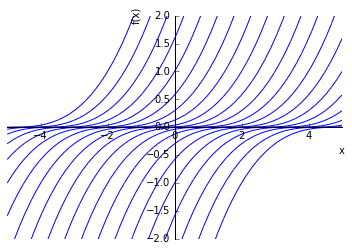
\includegraphics[scale=.4]{imagenes/no-unicidad.png}
 \end{tabular}




\section{Sistemas de Ecuaciones Diferenciales}
\subsection{Definición y ejemplos}
Un \emph{sistema de ecuaciones diferenciales de primer orden} es un conjunto  de ecuaciones que relacionan una variable independiente, digamos $x$, un conjunto de variables dependientes, digamos $y_1(x),\ldots,y_n(x)$, y sus derivadas respecto a $x$. A las ecuaciones diferenciales con una incognita y una ecuación las denominaremos \emph{ecuaciones escalares}.

\begin{definicion} Un sistema de ecuaciones diferenciales es una conjunto de ecuaciones de la forma
\begin{equation}\label{eq:sist_ecua}
\left\{
\begin{split}
 \frac{dy_1}{dx}(x)&=f_1(x,y_1(x),\ldots,y_n(x))\\
  \frac{dy_2}{dx}(x)&=f_2(x,y_1(x),\ldots,y_n(x))\\
       &\,\,\vdots                                   \\
 \frac{dy_n}{dx}(x)&=f_n(x,y_1(x),\ldots,y_n(x))\\
\end{split}\right.,
\end{equation}
donde $f_j:[a,b]\times\rr^n\to\rr$, $j=1,\ldots,n$, son funciones.

Una manera alternativa y compacta de denotar un sistema se logra introduciendo las funciones $y=(y_1,\ldots,y_n)$  y $f=(f_1,\ldots,f_n)$. Entonces $y:[a,b]\to\rr^n$ es una función con valores en $\rr^n$ y $f:[a,b]\times \rr^n\to\rr^n$ es un campo vectorial dependiente de $x$. Con estas notaciones el sistema se escribe:
\begin{equation}\label{eq:sist_ecua_comp}
 y'(x)=f(x,y(x)).
\end{equation}

\end{definicion}






\begin{ejemplo} [Ecuación del péndulo]{} Si $x(t)$ es el ángulo que forma un péndulo, de longitud $l$, con la vertical en el tiempo $t$ y $v(t)=x'(t)$, entonces $x(t)$ y$v(t)$ deben satisfacer el siguiente sistema de  ecuaciones:
\begin{equation}\label{eq:sist_pend}
\left\{
\begin{split}
 x'(t)&=v(t)\\
  v'(t)&=-\frac{g}{l}\sen(x(t)).\\
\end{split}\right.
\end{equation}


\end{ejemplo}


\begin{ejemplo}[Sistemas de ecuaciones de Lotka-Volterra]{}
 En 1925 y 1926, Alfred J. Lotka y Vito Volterra respectivamente, introdujeron
 las \href{https://es.wikipedia.org/wiki/Ecuaciones_Lotka%E2%80%93Volterra}{ecuaciones de Lotka-Volterra}. \marginpar{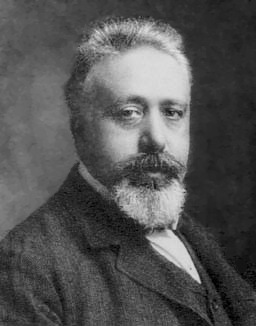
\includegraphics[scale=.28]{imagenes/Vito_Volterra.jpg}\\
 Vito Volterra (1860-1940)}  Se trata de un sistema de dos ecuaciones diferenciales de primer orden que se usan para describir dinámicas de sistemas biológicos en el que dos especies interactúan, una como presa y otra como depredador. Se definen como:
\begin{equation}\label{eq:lotka_volterra}
\left\{
\begin{split}
 x'(t) &= x(t) ( \alpha − \beta  y(t) )\\
  y'(t)&=-y(t)(\gamma-\delta x(t))\\
\end{split}\right.
\end{equation}
La variable $y$ representa el número de individuos de algún predador (por ejemplo, un lobo) y $x$ es el número de sus presas (por ejemplo, conejos), $t$ representa el tiempo; y  $\alpha,\beta,\gamma$ y $\delta$ son parámetros (positivos)

\end{ejemplo}


\subsection{Sistemas de ecuaciones y ecuaciones de orden superior}

\emph{Es posible convertir el sistema \eqref{eq:sist_ecua} de $n$-ecuaciones diferenciales de primer orden  en una ecuación escalar de orden $n$
\begin{equation}\label{eq:orden_n}
y^{(n)}=f(x,y,y',\ldots,y^{(n-1)}).
\end{equation}
y viceverza.}

Para justificar la aseveración anterior supongamos que $y=y(x)$ resuelven  \eqref{eq:orden_n} y escribamos:
\[y_1=y,\, y_2=y',\,y_3=y'',\ldots, y_{n}=y^{(n-1)}.\]
Entonces notar que
\begin{equation}\label{eq:sist_ecua_conv}
\left\{
\begin{array}{l l l}
 y_1'(x)&=y_2(x)\\
  y_2'(x)&=y_3(x)\\
       &\,\,\vdots\\
  y_{n-1}'(x)&=y_n(x)\\
 y_n'(x)&=f(x,y_1(x),\ldots,y_n(x))\\
\end{array}\right.,
\end{equation}

Reciprocamente, supongamos que $y_1,\ldots,y_n$ resuelven \eqref{eq:sist_ecua}. Por simplicidad vamos a suponer que las $f_j$ son independientes de $x$, el procedimiento general sigue las mismas líneas que el caso que discutimos aquí. Se toma $y=y_n$ (podríamos usar cualquier $y_j$, $j=1,\ldots,n$). Ahora derivamos sucesivamente $n$-veces respecto a $x$ la ecuación para $y_n$,  y reemplazamos cada derivada $y_j'$ por $f_j$ (vamos a omitir los argumentos de $f_j$ que son en todos los casos $(y_1,\ldots,y_n)$):

\[%\label{eq:sist_ecua_conv}
\begin{array}{c c c}
y_n'(x) =& f_n(y_1,\ldots,y_n) &\eqqcolon g_1(y_1,\ldots,y_n)\\
 y_n''(x)=&\sum\limits_{j=1}^n\frac{\partial f_n}{\partial y_j}f_j+
 & \eqqcolon g_2(y_1,\ldots,y_n)\\
  y_n'''(x)=&\sum\limits_{k,j=1}^n\frac{\partial^2 f_n}{\partial y_k \partial y_j}f_kf_j+
  \sum\limits_{k,j=1}^n\frac{\partial f_n}{\partial y_j}\frac{\partial f_j}{\partial y_k}f_k & \eqqcolon g_k(y_1,\ldots,y_n)\\
  &\,\,\vdots &\,\,\vdots \\
  y^{(n)}_n(x) =&\cdots & \eqqcolon g_n(y_1,\ldots,y_n)
  \\
\end{array}
\]
%\end{equation}
Las igualdades anteriores tienen la estructura $z=G(y)$, donde $y=(y_1,\ldots,y_n)$, $z=(y_n',y_n'',\ldots,y_n^{(n)})$ y $G=(y_1,\ldots,y_n)$. Si la función $G:\rr^n\to\rr^n$ es invertible y escribimos $H=G^{-1}$ entonces
\[y_n=H_n(z)=H_n(y_n',y_n'',\ldots,y_n^{(n)}).\]
La anterior es una ecuación escalar de orden $n$ para $y_n$. Por consiguiente hemos logrado reducir el sistema de $n$-ecuaciones a una ecuación de orden $n$. Observar que si resolvemos esta ecuación, encontrando $y_n$, podemos hallar el resto de las incognitas $y_j$, $j=1,\ldots,n-1$,  usando que $y_j=H_j(y_n',y_n'',\ldots,y_n^{(n)})$.


\begin{ejemplo}[Ecuaciones de Lotka-Volterra.]{} Reduzcamos las ecuaciones de Lotka-Volterra a una ecuación de orden 2 y luego revirtamos el camino.

La primera parte la resolvemos con Sympy:
\lstinputlisting[language=Python]{scripts/Sist-Ecua.py}
Resulta en
\begin{equation}\label{eq:lotka_escalar}\frac{d^{2}}{d t^{2}}  y{\left (t \right )- \frac{d}{d t} y{\left (t \right )} +
\left(- \alpha \gamma - \alpha\right) y{\left (t \right )} + \left(\beta \gamma + \beta\right) y^{2}{\left (t \right )} }=0
\end{equation}

El camino inverso es más sencillo. Llamamos $z=y'$. Usando las variables $y,z$ la ecuación \eqref{eq:lotka_escalar} se escribe
\[
 \left\{
 \begin{array}{ll}
    y'(t)&=v(t)\\
    v'(t)&=v+\left( \alpha \gamma + \alpha\right) y{\left (t \right )} - \left(\beta \gamma + \beta\right) y^{2}{\left (t \right )}
 \end{array}
 \right.
 \]

 No llegamos a la ecuación de partida. Hay que tener presente que una ecuación tiene diferentes representaciones en diferentes variables y que las variables que hemos elegido para el camino de vuelta $y,v$, no son las originales del problema $y,x$.


\end{ejemplo}


\section{Método de iteraciones de Picard}

En esta sección vamos a describir la estrategia que emplearemos para la demostración de la existencia de soluciones. El método que seguiremos fue ideado por \href{https://es.wikipedia.org/wiki/Charles_%C3%89mile_Picard}{Émile Picard} \marginpar{
    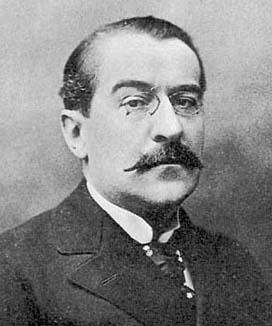
\includegraphics[scale=.3]{imagenes/Picard.jpg}\\
    Émile Picard (1856-1941)
}

Introducimos previamente algunas definiciones elementales.

\begin{definicion}
 Sea $\alpha$ una función  definida en un intervalo $[a,b]\subset \rr$ con valores en $\rr^n$, $n\geq 1$, tal que cada componete es una función integrable. Entonces, como es usual, escribimos
 \[\int_a^b\alpha(s)ds=\left(\int_a^b\alpha_1(s)ds,\ldots,\int_a^b\alpha_n(s)ds\right) \]
\end{definicion}

Es un ejercicio muy sencillo  demostrar que vales las propiedades elementales de las integrales, para esta extensión del concepto de integral a funciones con valores vectoriales. En particular vale el Teorema Fundamental del Cálculo: \emph{Si $\alpha$ es continuamente diferenciable entonces
\[ \int_a^b\alpha'(s)ds=\alpha(b)-\alpha(a).\]
}

Además vale la \emph{desigualdad triangular:} si $a<b$
\[\left\|\int_a^b \alpha(s)ds\right\|\leq \int_a^b \left\|\alpha(s)\right\|ds.\]
Nuestra intención es demostrar la existencia de soluciones de un PVI para el sistema de EDOs
\boxedeq{
\left\{
\begin{array}{ll}
 y'(x)&=f(x,y)\\
 y(x_0)&=y_0\\
\end{array}
\right. ,
}{eq:PVI_prin}

donde $f:\Omega \subset (a,b)\times \rr^n\to \rr^n$, $\Omega$ abierto, $y:(a,b)\to \rr^n$ (se debe satisfacer que $(x,y(x))\in \Omega$, para $x\in [a,b]$), $x_0\in (a,b)$
e $y_0\in\rr^n$ son dados con $(x_0,y_0)\in \Omega$.



Integremos la ecuación diferencial en un intervalo de extremos $x_0$ y $x$ y tomando en consideeración las condiciones iniciales obtenemos una nueva ecuación para $y(x)$,  en este caso una \href{https://es.wikipedia.org/wiki/Ecuaci%C3%B3n_integral}{ecuación integral} :

\boxedeq{
y(x)=y_0+\int_{x_0}^xf(t,y(t))dt.
}{eq:ecua_int}

Esta ecuación presenta una estructura muy particular. Podemos pensar el miembro derecho de \eqref{eq:ecua_int} como una trasformación (función) $T$ que lleva la función $y=y(x)$ en la función
\[
 T(y)(x):=y_0+\int_{x_0}^xf(t,y(t))dt.
\]
Pensando de esta manera  \eqref{eq:ecua_int} se escribe sencillamente
\[
 T(y)=y.
\]
Vale decir, la ecuación integral expresa el hecho que $T$ lleva a la función $y$ en si misma. Esto en matemática es conocido como un \href{https://es.wikipedia.org/wiki/M%C3%A9todo_del_punto_fijo}{punto fijo}. En análisis numérico los puntos fijos son utilizados para resolver ecuaciones algebraicas del tipo $h(x)=x$, donde $h:\rr\to\rr$. En aquel copntexto se ve que un procedimiento para aproximar soluciones es interar la función $h$, i.e. dado un $x_0$ cualquiera considerar la sucesión de \emph{aproximaciones sucesivas}
\[x_n=h(x_{n-1}),\quad n=1,2,\ldots.\]
El fundamento de proceder así es que si la sucesión $x_n$ converge a algún valor $x^*$ y si $h$ es continua entonces $x^*$ resuelve $h(x)=x$ pues
\begin{equation}
\label{eq:pto_fijo}h(x^*)=h\left(\lim_{n\to\infty} x_n\right)=\lim_{n\to\infty} h(x_n)=\lim_{n\to\infty} x_{n+1}=x^*.
\end{equation}

Vamos a proceder por analogía y proponer el siguiente proceso iterativo que genera las funciones $\varphi_k$, $k=0,1,\ldots$:

\boxedeq{
\left\{
\begin{array}{ll}
\varphi_0&=y_0\\
\varphi_{k+1}(x)&=y_0+\int_{x_0}^xf(t,\varphi_k(t))dt.\\
\end{array}
\right. .
}{eq:iter_picard}

Este proceso se denomina \emph{método de las aproximaciones sucesivas de Picard} y fué propuesto por E. Picard en  \cite{EmilePicard1893} y luego generalizado por \href{https://es.wikipedia.org/wiki/Ernst_Leonard_Lindel%C3%B6f}{Ernest Lindelöf}  en \cite{ErnestLindelof1894}. \marginpar{
    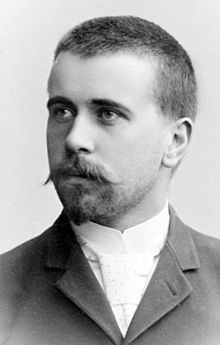
\includegraphics[scale=.3]{imagenes/Lindelof.jpg}\\
   Ernst L. Lindelöf (1870—1946)
}



Deberemos indagar por condiciones que nos aseguren que la sucesión $\varphi_k$ converja a una función $\varphi$ y que esta función $\varphi$ es solución del PVI. Antes de adentrarnos en los detalles de las demostraciones, constatemos que la idea funciona en algunos ejemplos sencillos.

\begin{ejemplo}{} Resolver
\[
 \left\{
 \begin{array}{ll}
 y'(x)&=y(x)\\
 y(0)&=y_0\\
 \end{array}
  \right. ,
\]
donde $y:\rr\to\rr$ e $y_0$ es un punto arbitrario de $\rr$.

Aplicando el método de picard:
\[
 \begin{array}{lll}
  \varphi_0(x)&=y_0 &\\
  \varphi_1(x) &= y_0+\int_{0}^x \varphi_0(t)dt &= y_0(1+x)\\
  \varphi_2(x) &= y_0+\int_{0}^x \varphi_1(t)dt &= y_0(1+x+\frac{x^2}{2})\\
               &\,\vdots                        &\,\vdots                 \\
  \varphi_k(x) &= y_0+\int_{0}^x \varphi_k(t)dt &= y_0(1+x+\cdots+\frac{x^k}{k!})\\
 \end{array}
\]
Se aprecia que en $\varphi_k$ aparecen las sumas parciales del desarrollo en serie de Taylor alrededor de $0$ de la función exponencial. Luego tenemos que $\varphi_k$ converge a $y_0e^x$ que es justamente la solución delm PVI propuesto.
\end{ejemplo}

Más ejemplos será tratados en la actividad práctica.

\section{\href{https://es.wikipedia.org/wiki/Teorema_del_punto_fijo_de_Banach}{Teorema de punto fijo Banach}}

\begin{definicion} Sea $(X,d)$ un espacio métrico completo. Una función $K:X\to X$ se denominará una contracción si existe un $\theta\in [0,1)$ tal que
\[d(K(x),K(y))\leq \theta d(x,y),\quad x,y\in X.\]
\end{definicion}

Dada una función $K:X\to X$ escribiremos
\[K^n(x)=\underbrace{K\left( K \left( K\cdots K(x)\cdots \right)\right)}_{n-\hbox{veces}}.\]
Cuando $n=0$ ponemos $K^0(x)=x$.

\begin{teorema}[Principio de contracción de Banach]{teo:banach}  Sea $(X,d)$ un espacio métrico completo y $K:X\to X$  una contracción. Entonces $K$ tiene un único punto fijo $x^*$. Además para todo $x$
\[d(K^n(x),x^*)\leq \frac{\theta^n}{1-\theta}d(K(x),x).\]
\end{teorema}\marginpar{
    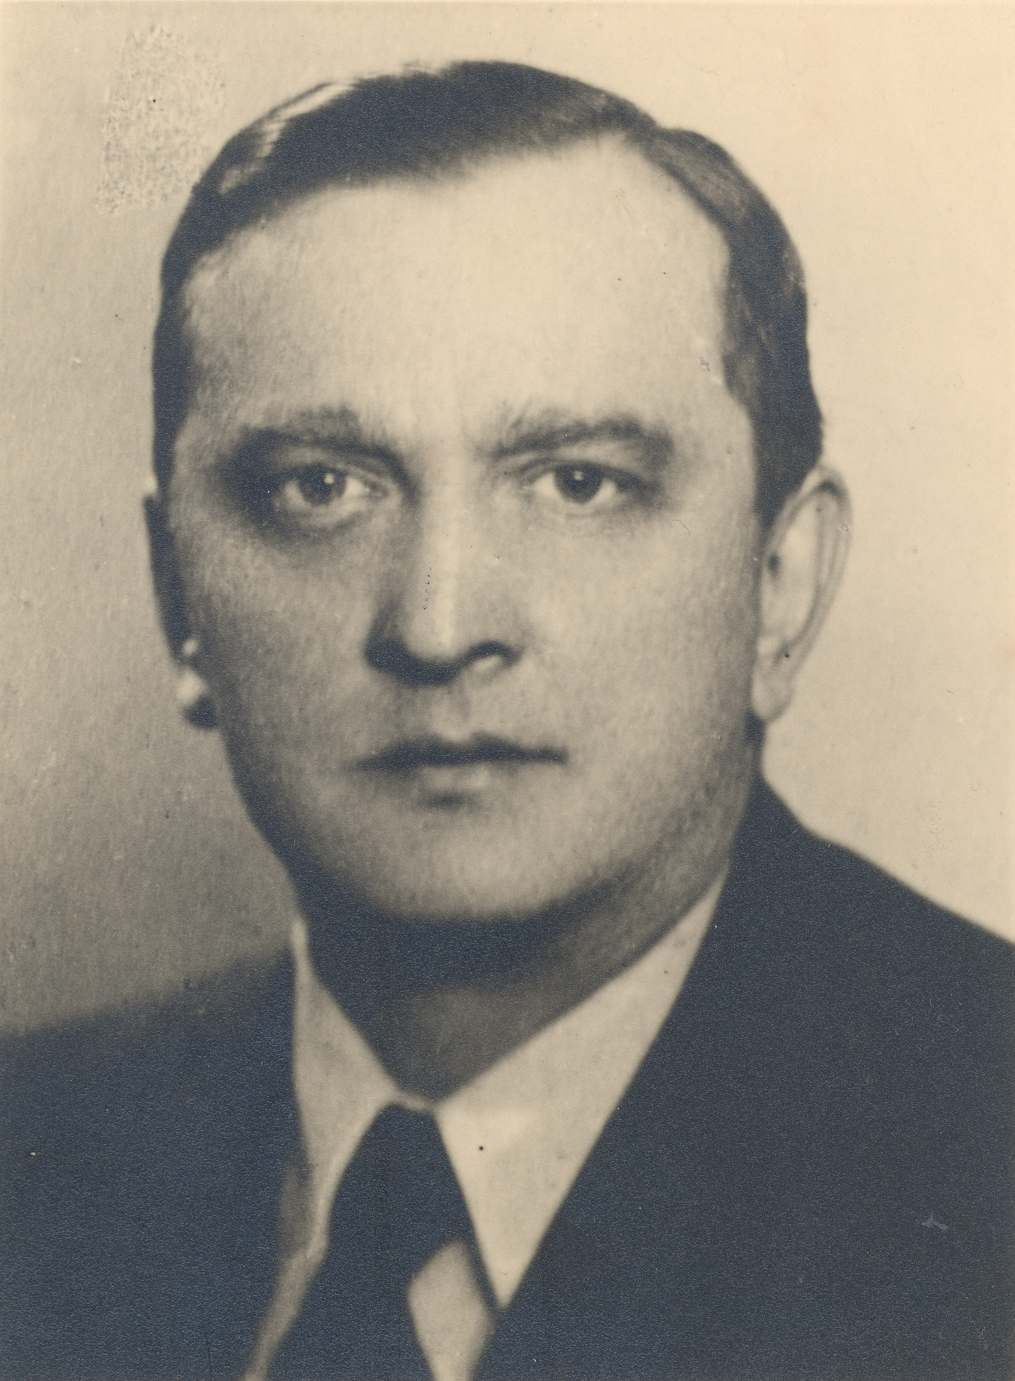
\includegraphics[scale=.3]{imagenes/banach.jpg}\\
   Stefan Banach (1892—1945)
}
\begin{proof} Sea $x\in X$ un punto arbitrario y definimos $x_n:=K^n(x)$. Entonces si $m<n$
\[
\begin{split}
 d(K^n(x),K^m(x))&\leq d(K^n(x),K^{n-1}(x))+\cdots+ d(K^{m+1}(x),K^m(x))\\
 &\leq \theta^{n-1} d(K(x),x)+\cdots + \theta^m d(K(x),x)\\
 &\leq \frac{\theta^m}{1-\theta}d(K(x),x)
 \end{split}
\]
Como $\theta<1$ vemos que si $m,n$ son suficientemente grandes podemos hacer que $ d(K^n(x),K^m(x))$ sea arbitrariamente chico. Hemos probado que la sucesión $K^n(x)$ es de Cauchy, de allí tiene límite, al que llamaremos $x^*$. Que $x^*$ es punto fijo se justifica como en \eqref{eq:pto_fijo} (notar que una contracción es continua).

Que el punto fijo es único, se deduce de suponer que existe otro $z^*$ y aplicar lque $K$ es contracción
\[d(x^* , z^*)=d(K(x^*) , K(z^*))\leq \theta d(x^* , z^*)<d(x^* , z^*).\]
Lo que es una contradicción.
\end{proof}

\begin{corolario}{cor:banach}  Sea $(X,d)$ un espacio métrico completo y $K:X\to X$ continua y $K^m$ contracción para algún $m\in\mathbb{N}$. Entonces $K$ tiene un único punto fijo $x^*$ y para todo $x\in X$ se tiene
\[ \lim_{n\to\infty} K^n(x)=x^*.\]
 \end{corolario}
 
 \begin{proof} Sea $x^*$ el único punto fijo de $K^m$ dado por el principio de contracción de Banach aplicado a $K^m$. Sean $x\in X$ y $0\leq r<m$. Consideremos las sucesiones $\{K^{km+r}(x)\}_{k\in\mathbb{N}}$. Tenemos $m$ de estas sucesiones, una para cada valor de $r=0,\ldots,m-1$. Todas ellas son subsucesiones de $\{K^n(x)\}_{n\in\mathbb{N}}$. Además 
  \[\bigcup_{r=0}^{m-1}\{K^{km+r}(x)\}_{k\in\mathbb{N}}=\{K^n(x)\}_{n\in\mathbb{N}}.\]
  Vamos a demostrar que estas $m$ subsucesiones convergen todas a $x^*$. Esto es facil consecuencia de que $K^m$ es contracción. Pues de ello obtenemos que $\left(K^{m}\right)^n(y)\to x^*$, cuando $n\to\infty$ para todo $y\in X$. Luego
  \[\lim_{k\to\infty}K^{km+r}(x)=\lim_{k\to\infty}\left(K^{m}\right)^k(K^r(x))=x^*.\]
  Esto establece que $ \lim_{n\to\infty} K^n(x)=x^*$.
  
  Veamos que $x^*$ es punto fijo de $K$. 
  \[K(x^*)=K\left(\lim_{n\to\infty} K^{n}(x)\right)=\lim_{n\to\infty} K\left( K^{n}(x)\right)
  =\lim_{n\to\infty}  K^{n+1}(x)=x^*.\]
  
  Para la unicidad, observar que un punto fijo de $K$ lo es de $K^m$. Cómo $K^m$ tiene un único punto fijo, lo mismo podemos afirmar de $K$.
  
 \end{proof}


\begin{definicion} Sea $f:\Omega \subset \rr^n\to \rr^m$. Diremos que $f$ es \emph{lipschitziana} (o que es una función Lipschitz) si existe una constante $K\geq 0$ tal que
\[\|f(x)-f(y)\|\leq K\|x-y\|,\quad \forall x,y\in \Omega .\]

Si $f:\Omega\subset\rr\times \rr^n\to\rr^m$, diremos que $f=f(t,x)$ es lipschitziana respecto a la segunda variable si existe  $K\geq 0$ tal que
\[\|f(t,x)-f(t,y)\|\leq K\|x-y\|,\quad \forall (t,x),(t,y)\in \Omega .\]
 
\end{definicion}



\begin{teorema}[Picard- Lindelöf]{teo:picard} Sean $x_0\in\rr$, $y_0\in\rr^n$ y $f:\Omega\to\rr^n$ continua y lipschitziana respecto a la segunda variable, donde $\Omega=I_a\times B_b$,  $I_a=[x_0-a,x_0+a]$ y $B_b=\{y\in\rr^n|\|y-y_0\|\leq b\}$. Como $\Omega$ es compacto y $f$ es continua, existe $M\geq 0$ tal que $\|f\|\leq M$. Entonces existe una única solución del PVI:
\[
 \left\{\begin{array}{ll}
	  y'(x)&=f(x,y(x)),\\
	  y(x_0)&=y_0\\         
        \end{array}
\right. ,
\]
en $I_{\delta}=(x_0-\delta,x_0+\delta)$ con $\delta:=\min\{a,b/M\}$.
 \end{teorema}

 \begin{proof}
 
 Definamos
\[X=C(I_{\delta},B_b):=\{\varphi| \varphi:I_a\to B_b\hbox{ continua }\}.\]
\begin{figure}[h]
  \begin{center}
\scalebox{.6} % Change this value to rescale the drawing.
{
\begin{pspicture}(0,-4.81)(10.393595,4.81)
\definecolor{color123b}{rgb}{0.9098039215686274,0.8431372549019608,0.8431372549019608}
\definecolor{color105b}{rgb}{0.8627450980392157,0.7607843137254902,0.7607843137254902}
\psellipse[linewidth=0.04,linestyle=dashed,dash=0.16cm 0.16cm,dimen=outer,fillstyle=solid,fillcolor=color105b](3.86,0.85)(0.44,1.3)
\psellipse[linewidth=0.04,linestyle=dashed,dash=0.16cm 0.16cm,dimen=outer](5.04,0.88)(0.4,1.29)
\psellipse[linewidth=0.04,linestyle=dashed,dash=0.16cm 0.16cm,dimen=outer,fillstyle=solid,fillcolor=color123b](6.07,0.86)(0.39,1.31)
\pspolygon[linewidth=0.04](0.0,-4.79)(0.04231884,2.37)(2.92,4.79)(2.86,-2.55)(2.88,-2.49)
\psbezier[linewidth=0.04](1.42,2.19)(0.96,2.05)(0.94,1.23)(0.92,0.93)(0.9,0.63)(0.92,-0.31)(1.42,-0.39)
\psbezier[linewidth=0.04,linestyle=dashed,dash=0.16cm 0.16cm](1.48,-0.41)(1.98,-0.27)(1.98,0.51)(1.98,0.93)(1.98,1.35)(1.9,2.27)(1.48,2.15)
\psline[linewidth=0.04cm](1.44,2.17)(7.1,2.15)
\psline[linewidth=0.04cm](1.44,-0.41)(7.02,-0.43)
\psellipse[linewidth=0.04,dimen=outer](7.0,0.86)(0.54,1.29)
\psline[linewidth=0.04cm,linestyle=dashed,dash=0.16cm 0.16cm](7.0,0.83)(1.46,0.81)
\psdots[dotsize=0.24](7.06,0.83)
\psdots[dotsize=0.12](1.5,0.83)
\psline[linewidth=0.04cm,arrowsize=0.05291667cm 2.0,arrowlength=1.4,arrowinset=0.4]{->}(1.5,0.77)(1.78,1.97)
\psline[linewidth=0.04cm,arrowsize=0.05291667cm 2.0,arrowlength=1.4,arrowinset=0.4]{->}(1.3,-1.77)(9.52,-1.71)
\usefont{T1}{ptm}{m}{n}
\rput(2.4290624,3.5){$\mathbb{R}^n$}
\usefont{T1}{ptm}{m}{n}
\rput(1.3590626,1.48){$b$}
\psline[linewidth=0.04cm,linestyle=dashed,dash=0.16cm 0.16cm](5.04,0.83)(5.0,-1.77)
\psline[linewidth=0.04cm,linestyle=dashed,dash=0.16cm 0.16cm](7.1,0.79)(7.1,-1.83)
\psline[linewidth=0.04cm,linestyle=dashed,dash=0.16cm 0.16cm](3.9,0.87)(3.86,-1.79)
\usefont{T1}{ptm}{m}{n}
\rput(5.0590625,-1.96){$x_0$}
\usefont{T1}{ptm}{m}{n}
\rput(6,-1.96){$x_0+\delta$}
\usefont{T1}{ptm}{m}{n}
\rput(3.8490624,-1.96){$x_0-\delta$}
\usefont{T1}{ptm}{m}{n}
\rput(1.5590626,0.52){$y_0$}
\psbezier[linewidth=0.04,arrowsize=0.05291667cm 2.0,arrowlength=1.4,arrowinset=0.4]{->}(6.4,3.39)(5.6,3.05)(6.6,2.49)(5.52,1.77)
\usefont{T1}{ptm}{m}{n}
\rput(6.4590626,3.42){$\Omega$}
\usefont{T1}{ptm}{m}{n}
\rput(9.049064,-1.48){$\mathbb{R}$}
\psline[linewidth=0.04cm,linestyle=dashed,dash=0.16cm 0.16cm](6.06,0.79)(6.08,-1.71)
\usefont{T1}{ptm}{m}{n}
\rput(7.2690625,-1.94){$x_0+a$}
\psbezier[linewidth=0.04,arrowsize=0.05291667cm 2.0,arrowlength=1.4,arrowinset=0.4]{->}(4.36,2.51)(4.5,1.53)(5.48,2.21)(5.12,0.95)
\psdots[dotsize=0.2](5.06,0.79)
\usefont{T1}{ptm}{m}{n}
\rput(4.2745314,2.78){$(x_0,y_0)$}
\end{pspicture} 
}
 \caption{Conjunto $I_{\delta}\times B_b$}\label{fig:exi_uni}
  \end{center}
\end{figure}
\begin{ejercicio} La función
\[d(\varphi_1,\varphi_2):=\max\left\{\|\varphi_1(x)-\varphi_2(x)\| \,\big| x\in I_{\delta}\right\}\]
  define una métrica sobre el conjunto $X$ y con esta métrica $(X,d)$ es completo. 
\end{ejercicio}

Para $\varphi\in X$, definamos una nueva función $K(\varphi)$ por:
\[K(\varphi)(x)=y_0+\int_{x_0}^xf(t,\varphi(t))dt.\]
\noindent\textbf{Afirmación 1:} $K:X\to X$. 

En efecto, si $x\geq x_0$ y $x\in I_{\delta}$ (si $x\leq x_0$ queda como ejercicio)
\[\|K(\varphi)(x)-y_0\|\leq \int_{x_0}^x\|f(t,\varphi(t))\|dt\leq M|x-x_0|\leq b.\]
Esto muestra que $K(\varphi):I_{\delta}\to B_b$. 

La continuad se establece del siguiente modo. Si $x_1<x_2$
\[
\|K(\varphi)(x_1)-K(\varphi)(x_2)\|\leq \int_{x_1}^{x_2}\|f(t,\varphi(t))\|dt\leq M|x_1-x_2|.\]

Lo que implica la continuidad. Entonces $K(\varphi)\in X$. 

\noindent\textbf{Afirmación 2:} $K^m$ es  contracción para $m$ suficientemente grande. 

La afirmación es consecuencia de la siguiente desigualdad, para $\varphi_1,\varphi_2\in X$ y $x\in I_{\delta}$
\[\|K^m(\varphi_1)(x)-K^m(\varphi)(x)\|\leq \frac{K^m|x-x_0|^m}{m!}d(\varphi_1,\varphi_2).\]
La prueba procede por induccón sobre $m$. Cuando $m=0$ es inmediata. Supuesta válida la desigualdad para $m$ vemos que (otra vez asumimos $x_0\leq x$)

\[
  \begin{split}
    \|K^{m+1}(\varphi_1)(x)&-K^{m+1}(\varphi)(x)\|=   \|K\left(K^{m}(\varphi_1)\right)(x)-K\left(K^{m}(\varphi)\right)(x)\|\\
    &=\left\|   
    \int_{x_0}^{x} f(t,K^m(\varphi_1)(t))- f(t,K^m(\varphi_2)(t)) dt
        \right\|\\
     &\leq    
    \int_{x_0}^{x} \left\|f(t,K^m(\varphi_1)(t))- f(t,K^m(\varphi_2)(t))\right\| dt\\
    &\leq     K\int_{x_0}^{x} \left\|K^m(\varphi_1)(t)- K^m(\varphi_2)(t))\right\| dt\\
    &\leq  \frac{K^{m+1}}{m!}d(\varphi_1,\varphi_2) \int_{x_0}^{x}  |t-x_0|^m dt\\
    &=\frac{K^{m+1}|x-x_0|^{m+1}}{(m+1)!}d(\varphi_1,\varphi_2)
  \end{split}
\]

Notar que $K^m|x-x_0|^m/m!$ es el valor absoluto del término general de la serie de Taylor de $e^{Kx}$ alrededor de $x_0$.Como esta serie tiene radio de convergencia infinito, el término general tiende a cero. Por consiguiente existe $m$ suficientemente grande para que $K^m|x-x_0|^m/m!<1$. Para este $m$, $K^m$ será contracción. Luego, por el Corolario \ref{cor:banach},  deducimos que $K$ tiene un único punto fijo. Vale decir que existe $y\in X$ con
\[
 y(x)=y_0+\int_{x_0}^xf(t,y(t))dt.
\]
Notar que $y(x_0)=y_0$, i.e. $y$ satisface la condición inicial. Por el teorema fundamental del cálculo $y'(x)=f(x,y(x))$, i.e. $y$ satisface la ecuación y por tanto, finalmente, es solución del PVI.\end{proof}


\begin{corolario}{} Sea $\Omega$ abierto de $\rr\times \rr^n$ y $f:\Omega\to\rr^n$ continua con $\partial f_j/\partial y_k)$ tambien continuas $j,k=1,\ldots,n$. Entonces para todo $(x_0,y_0)\in\Omega$ existe un entorno $V=[x_0-\delta,x_0+\delta]\times B_b(y_0)$ tal que el PVI
 \[
 \left\{\begin{array}{ll}
	  y'(x)&=f(x,y(x)),\\
	  y(x_0)&=y_0\\         
        \end{array}
\right. ,
\]
tiene solución única en $[x_0-\delta,x_0+\delta]$. Además el gráfico de esta solución está contenido en $V$..
\end{corolario}

\begin{proof} Sea $(x_0,y_0)\in\Omega$ arbitrario. Como $\Omega$ es abierto, existen $a,b>0$ tal que $[x_0-a,x_0+a]\times B_b(y_0)\subset \Omega$. Como $\partial f_j/\partial y_k)$ son continuas y $V$ es compacto, tenemos que existe $M>0$ con $|\partial f_j/\partial y_k)|\leq M$ en $V$, $j,k=1,\ldots,n$. El Teorema del valor medio para funciones en varias variables implica que existe una constante $C>0$ tal que si $(t,x),(t,z)\in V$
\[\|f(t,x)-f(t,z)\|\leq C M\|x-z\|.\]
i.e. $f$ es Lipschitziana respecto a la segunda variable en $V$. La conclusión del Corolario sigue del Teorema de Picard- Lindelöf. 
\end{proof}


   
\nocite{JorgeSotomayor513}.




  \bibliographystyle{apalike}
  \bibliography{diferenciales_ecuaciones,diferenciales_ecuaciones_sim}
% \documentclass{article}
%\documentclass[hyperref={colorlinks=true}]{beamer}
%\documentclass[handout,hyperref={colorlinks=true}]{beamer}


%%%%%%%%%%%%%%%%%%%%%%%%%%%%%%Paquetes%%%%%%%%%%%%%%%%%%%%%%%%%%%%%%%%%%%%%%%%%%%%%%%5
%%%%%%%%%%%%%%%%%%%%%%%%%%%%%%%%%%%%%%%%%%%%%%%%%%%%%%%%%%%%%%%%%%%%%%%%%%%%%%%%%%%%%
\usepackage{empheq}
\usepackage[spanish]{babel}
%\usepackage[utf8x]{inputenc}
\usepackage{times}
%\usepackage[T1]{fontenc}
\usepackage[latin1]{inputenc}
\usepackage{amssymb,amsmath,amsthm}
\usepackage{enumerate}
\usepackage{verbatim}
\usepackage{ esint }
%\usepackage{pst-all}
%\usepackage{pstricks-add}
\usepackage{array}
%\usepackage[T1]{fontenc}
\usepackage{animate}
%\usepackage{media9}
\usepackage{xparse}
\usepackage{listings}
\usepackage{ wasysym }
%\usepackage{sagetex}
\usepackage{yfonts,mathrsfs,eufrak}
\usepackage{hyperref}
\usepackage{color}
\usepackage{url}
\usepackage{theorem}
\usepackage{boiboites}
\usepackage{wrapfig}
\usepackage{ esint }
\definecolor{mygreen}{rgb}{0,0.6,0}
\definecolor{mygray}{rgb}{0.5,0.5,0.5}
\definecolor{mymauve}{rgb}{0.58,0,0.82}

\lstset{ %
  backgroundcolor=\color{white},   % choose the background color; you must add \usepackage{color} or \usepackage{xcolor}
  basicstyle=\footnotesize,        % the size of the fonts that are used for the code
  breakatwhitespace=false,         % sets if automatic breaks should only happen at whitespace
  breaklines=true,                 % sets automatic line breaking
  captionpos=b,                    % sets the caption-position to bottom
  commentstyle=\color{mygreen},    % comment style
  deletekeywords={...},            % if you want to delete keywords from the given language
  escapeinside={\%*}{*)},          % if you want to add LaTeX within your code
  extendedchars=true,              % lets you use non-ASCII characters; for 8-bits encodings only, does not work with UTF-8
  frame=single,	                   % adds a frame around the code
  keepspaces=true,                 % keeps spaces in text, useful for keeping indentation of code (possibly needs columns=flexible)
  keywordstyle=\color{blue},       % keyword style
  language=Python,                 % the language of the code
  otherkeywords={*,...},           % if you want to add more keywords to the set
  numbers=left,                    % where to put the line-numbers; possible values are (none, left, right)
  numbersep=5pt,                   % how far the line-numbers are from the code
  numberstyle=\tiny\color{mygray}, % the style that is used for the line-numbers
  rulecolor=\color{black},         % if not set, the frame-color may be changed on line-breaks within not-black text (e.g. comments (green here))
  showspaces=false,                % show spaces everywhere adding particular underscores; it overrides 'showstringspaces'
  showstringspaces=false,          % underline spaces within strings only
  showtabs=false,                  % show tabs within strings adding particular underscores
  stepnumber=2,                    % the step between two line-numbers. If it's 1, each line will be numbered
  stringstyle=\color{mymauve},     % string literal style
  tabsize=2,	                   % sets default tabsize to 2 spaces
  title=\lstname                   % show the filename of files included with \lstinputlisting; also try caption instead of title
}


%%%%%%%%%%%%%%%%%%%%%%%%%%Nuevos comandos entornos%%%%%%%%%%%%%%%%%%%%%%%%%%%%%%%%
%%%%%%%%%%%%%%%%%%%%%%%%%%%%%%%%%%%%%%%%%%%%%%%%%%%%%%%%%%%%%%%%%%%%%%%%
\newenvironment{demo}{\noindent\emph{Dem.}}{$\square$ \newline\vspace{5pt}}

\newcommand{\com}{\mathbb{C}}
\newcommand{\dis}{\mathbb{D}}
\newcommand{\rr}{\mathbb{R}}
\newcommand{\oo}{\mathcal{O}}
%\renewcommand{\emph}[1]{\textcolor[rgb]{1,0,0}{#1}}
\newcommand{\der}[2]{\frac{\partial #1}{\partial #2}}
\renewcommand{\v}[1]{\overrightarrow{#1}}
\renewcommand{\epsilon}{\varepsilon}
%\newcommand{\defverbatim}{\def{#1}}
\renewcommand{\b}[1]{\boldsymbol{#1}}
\renewenvironment{frame}[1]{}{}
%\newcommand{\end{proof}}{$\square$}
\DeclareMathOperator{\atan2}{atan2}
\DeclareMathOperator{\sen}{sen}


%%%%%%%%%%%%%%%%%%%%%%%%Colores
\definecolor{myblue}{rgb}{.8, .8, 1}
\definecolor{dblackcolor}{rgb}{0.0,0.0,0.0}
\definecolor{dbluecolor}{rgb}{0.01,0.02,0.7}
\definecolor{dgreencolor}{rgb}{0.2,0.4,0.0}
\definecolor{dgraycolor}{rgb}{0.30,0.3,0.30}
\newcommand{\dblue}{\color{dbluecolor}\bf}
\newcommand{\dred}{\color{dredcolor}\bf}
\newcommand{\dblack}{\color{dblackcolor}\bf}


%%%%%%%%%%Definimos una caja con color
\newlength\mytemplen
\newsavebox\mytempbox
\makeatletter
\newcommand\mybluebox{%
\@ifnextchar[%]
{\@mybluebox}%
{\@mybluebox[0pt]}}
\def\@mybluebox[#1]{%
\@ifnextchar[%]
{\@@mybluebox[#1]}%
{\@@mybluebox[#1][0pt]}}
\def\@@mybluebox[#1][#2]#3{
\sbox\mytempbox{#3}%
\mytemplen\ht\mytempbox
\advance\mytemplen #1\relax
\ht\mytempbox\mytemplen
\mytemplen\dp\mytempbox
\advance\mytemplen #2\relax
\dp\mytempbox\mytemplen
\colorbox{myblue}{\hspace{1em}\usebox{\mytempbox}\hspace{1em}}}
\makeatother
\DeclareDocumentCommand\boxedeq{ m g }{%
{\begin{empheq}[box={\mybluebox[2pt][2pt]}]{equation}% #1%
\IfNoValueF {#2} {\label{#2}}%
#1
\end{empheq}
}%
}


%%%%%%%%%%%%%%%%%%
\newboxedtheorem[boxcolor=orange, background=blue!5, titlebackground=blue!20,
titleboxcolor = black,thcounter=section]{problema}{Problema}{thcounter1}

\newboxedtheorem[boxcolor=orange, background=blue!5, titlebackground=blue!20,
titleboxcolor = black,thcounter=section]{teorema}{Teorema}{thcounter2}

\newboxedtheorem[boxcolor=orange, background=blue!5, titlebackground=blue!20,
titleboxcolor = black,thcounter=section]{definicion}{Definici\'on}{thcounter3}

\newboxedtheorem[boxcolor=orange, background=blue!5, titlebackground=blue!20,
titleboxcolor = black,thcounter=section]{lema}{Lema}{thcounter4}

\newboxedtheorem[boxcolor=orange, background=blue!5, titlebackground=blue!20,
titleboxcolor = black,thcounter=section]{corolario}{Corolario}{thcounter5}

\newboxedtheorem[boxcolor=orange, background=blue!5, titlebackground=blue!20,
titleboxcolor = black,thcounter=section]{proposicion}{Proposici\'on}{thcounter6}

\newboxedtheorem[boxcolor=orange, background=blue!5, titlebackground=blue!20,
titleboxcolor = black,thcounter=section]{codigo}{Funci�n SymPy}{}




\newcounter{ejemplo_cont}
\setcounter{ejemplo_cont}{1}

\newenvironment{ejemplo}{\noindent\textbf{Ejemplo  \arabic{ejemplo_cont}.} }{\addtocounter{ejemplo_cont}{1}}
%%%%%%%%%%%%%%%%%%%%%%%%%%%%%%%%%%%%%%%%%%%%%%%%%%%%%%%%%%%%%%%%%%%%%%%%%%%%%%%%%%%%%%%%%%%%%%%%%%%%%%%%%%%
%%%%%%%%%%Para escibir en clase articulo o similar






\title{Ecuaciones Lineales de Segundo Orden}
\date{}

\begin{document}




\tableofcontents




\section{Introducci�n}


\begin{quote}
``Me convert� en ateo porque como estudiante de  post-grado en f�sica cu�ntica, la vida parec�a ser reducible a ecuaciones diferenciales de segundo orden. Matem�ticas, qu�mica y f�sica ten�an todo y yo no veo ninguna necesidad de ir m�s all� de eso.''
\end{quote}
\begin{flushright}
Francis Collins
\end{flushright}

 


\begin{definicion}[Ecuaci�n lineal general de segundo orden]
 \boxedeq{\frac{d^2y}{dx^2}+p(x)\frac{dy}{dx}+q(x)y=r(x),}{ec_2_gen}
donde $p,q,r$ son funciones definidas en un intervalo $I=(a,b)$ de $\rr$ con valores en $\rr$.Si $r\equiv 0$ se llama homog�nea
\boxedeq{\frac{d^2y}{dx^2}+p(x)\frac{dy}{dx}+q(x)y=0,}{ec_2_gen_hom}
\end{definicion}







\begin{teorema}[Teorema de existencia y unicidad de soluciones]
Supongamos $p,q,r$ continuas sobre $I$. Sean $x_0\in I$ e $y_0,y_1\in\rr$ dados. Entonces existe una �nica soluci�n del PVI
\[\left\{
\begin{array}{l l l}
\frac{d^2y}{dx^2}+&p(x)\frac{dy}{dx}+q(x)y=r(x),&x\in I\\
y(x_0)&=y_0&\\
y'(x_0)&=y^1_0&\\
\end{array}\right.
\]
\end{teorema}
\begin{proof} M�s adelante.

\end{proof}


\section{Estructura del conjunto de soluciones}
\begin{teorema}
Si $y_1$ e $y_2$ son soluciones de \eqref{ec_2_gen_hom} y $c_1,c_2\in\rr$ entonces $c_1y_1+c_2y_2$ es soluci�n. Vale decir, el conjunto de soluciones
es un espacio vectorial. En particular $y\equiv 0$ es una soluci�n, a la que llameremos \emph{trivial}.
\end{teorema}

\begin{proof}
 El operador
\[L[y]:=y''+py'+qy\]
es lineal, por consiguiente
$L[c_1y_1+c_2y_2]=c_1L[y_1]+c_2L[y_2]=0.$
\end{proof}


\begin{teorema}
 Supongamos que $y_p$ es una soluci�n particular de \eqref{ec_2_gen} y que $y_g=y_g(x,c_1,c_2)$ es una soluci�n
general de \eqref{ec_2_gen_hom}. Entonces $y=y_p+y_g$ es soluci�n general de \eqref{ec_2_gen}.
\end{teorema}



\begin{proof}
El operador
\[L[y]:=y''+py'+qy\]
es lineal, por consiguiente
$L[y_g+y_p]=L[y_g]+L[y_p]=0+r=r.$
Rec�procamente supongamos $y$ soluci�n de $L[y]=r$, entonces
$L[y-y_p]=L[y]-L[y_p]=r-r=0.$
Luego debe haber $c_1$ y $c_2$ con $y(x)-y_p(x)=y_g(x,c_1,c_2)$.

\end{proof}


Volviendo a las ecuaciones homog�neas, supongamos que tenemos dos soluciones de \eqref{ec_2_gen_hom} $y_1$ e $y_2$. Entonces la expresi�n
\begin{equation}\label{comb_lin}
c_1y_1+c_2y_2,\quad c_1,c_2\in\rr
\end{equation}
es soluci�n tambi�n. Notar que en la expresi�n aparecen dos constantes y hab�amos dicho que era de esperar que la soluci�n general de una ecuaci�n de orden 2 contuviese
precisamente dos constantes de integraci�n. De modo que podemos conjeturar que \eqref{comb_lin} es soluci�n general de \eqref{ec_2_gen_hom}.
Hay una situaci�n especial, si, por ejemplo, $y_1=ky_2$, $k\in\rr$,entonces $c_1y_1+c_2y_2=(c_1k+c_2)y_2=cy_2$. Vale decir la combinaci�n lineal \eqref{comb_lin}
termina siendo s�lo combinaci�n lineal de la funci�n $y_2$ y por ende siendo esencialmente una expresi�n uniparam�trica.

\begin{definicion}[Independencia lineal]
 Un conjunto finito de funciones $\{y_1,\ldots,y_n\}$ se dir� linealmente independiente sobre un conjunto $I$,
si la �nica soluci�n de $c_1y_1(t)+\cdots+c_ny_n(t)=0$, para $t\in I$, es $c_1=c_2=\cdots=c_n=0$.

\end{definicion}




\begin{definicion}[Definici�n wronskiano]
 Dadas $n$ fuciones $\{y_1,\ldots,y_n\}$ con dominio $I$ el wronskiano $W(x)=W(y_1,y_2,\ldots,y_n)(x)$ de estas funciones en un punto $x\in I$ se define por
\boxedeq{W(x)=\det\begin{pmatrix}
y_1(x) & y_2(x) & \cdots &y_n(x)\\
y_1'(x) & y_2'(x) & \cdots &y_n'(x)\\
\vdots & \vdots &\ddots& \vdots\\
y_1^{(n-1)}(x) & y_2^{(n-1)}(x) & \cdots &y_n^{(n-1)}(x)\\
\end{pmatrix}}{wronskiano}
\end{definicion}




\begin{lema}[Propiedades Wronskiano I]
 Sea $\{y_1,\ldots,y_n\}$ un conjunto de $n$ funciones. Si existe un $x_0\in I$ con $W(x_0)\neq 0$ entonces $\{y_1,\ldots,y_n\}$ son
linealmente independientes
\end{lema}


\begin{proof} Supongamos que $c_1y_1+\cdots+c_ny_n\equiv 0$. Derivando $n-1$ veces esta igualdad y evaluando el resultado en $x_0$ obtenemos
\[
\begin{split}
c_1y_1(x_0)+\cdots+c_ny_n(x_0)&=0\\
c_1y_1'(x_0)+\cdots+c_ny'_n(x_0)&=0\\
\vdots \quad& \quad\vdots\\
c_1y_1^{(n-1)}(x_0)+\cdots+c_ny^{(n-1)}_n(x_0)&=0\\
\end{split}
\]
Las igualdades anteriores dicen que el vector $(c_1,\ldots,c_n)^t$ pertenece al nucleo de la matriz
\[
\begin{pmatrix}
y_1(x_0) & y_2(x_0) & \cdots &y_n(x_0)\\
y_1'(x_0) & y_2'(x_0) & \cdots &y_n'(x_0)\\
\vdots & \vdots &\ddots& \vdots\\
y_1^{(n-1)}(x_0) & y_2^{(n-1)}(x_0) & \cdots &y_n^{(n-1)}(x_0)\\
\end{pmatrix}
\]
Como por hip�tesis la matr�z es no singular, debe ocurrir que $c_1=c_2=\cdots c_n=0$.
\end{proof}

\begin{teorema}[Teorema. Propiedades wronskiano II, F�rmula de Abel]
 Supongamos que $y_1$ e $y_2$ son soluci�n de
\begin{equation}\label{eq2orden}\frac{d^2y}{dx^2}+p(x)\frac{dy}{dx}+q(x)y=0,\quad x\in I=(a,b)\end{equation}
Entonces existe $c\in\rr$ que satisface
\boxedeq{W(y_1,y_2)(x)=ce^{-\int p dx}.}{formu_abel}
Esta expresi�n se denomina \href{http://en.wikipedia.org/wiki/Abel's_identity}{f�rmula de Abel}. En particular vale que
\[\exists x_0\in I: W(x_0)\neq 0 \Longleftrightarrow \forall x\in I: W(x)\neq 0 .\]
\end{teorema}

\begin{proof} Tenemos que
\[W(x)=y_1(x)y_2'(x)-y_1'(x)y_2(x).\]
Derivando y usando \eqref{eq2orden}
\[\begin{split}W'(x)&=y_1y_2''-y_1y_2''\\
&=y_1(-py_2'-qy_2)-y_2(-py_1'-qy_1)\\
&=-pW.
\end{split}
\]
Vale decir $W$ resuelve la ecuaci�n $W'=-pW$ la cual es facilmente resoluble, mostrando su resoluci�n que se satisface \eqref{formu_abel}
\end{proof}

\begin{teorema}[Propiedades wronskiano III]
 Sean $y_1$ e $y_2$ soluciones de \eqref{eq2orden}. Entonces son equivalentes
\begin{enumerate}
\item\label{item1} $y_1$ e $y_2$ son linealmente indepenientes en $I$.
\item\label{item2} $W(y_1,y_2)(x)\neq 0$ para todo $x\in I$.
\end{enumerate}
\end{teorema}


\begin{proof} Que \ref{item2} implica \ref{item1} es consecuencia de la propiedad del wronskiano I.
Veamos que \ref{item1} implica \ref{item2}. Supongamos que exista un $x_0$ con $W(x_0)=0$. Esto quiere decir que una de las columnas
de la matr�z wronskiana en $x_0$ es m�ltiplo de la otra. Supongamos que $y_2(x_0)=ky_1(x_0)$ e $y'_2(x_0)=ky'_1(x_0)$. Esto quiere decir que $y_2$ y $ky_1$
resuelven el mismo pvi. Por lo tanto $y_2(x)=ky_1(x)$ para todo $x$. Lo que nos dice lo contrario de \ref{item1}
\end{proof}


\begin{teorema}[Estructura del conjunto de soluciones, ecuaci�n  homog�nea]
 Si $y_1$ e $y_2$ son soluciones linealmente independientes de
\[\frac{d^2y}{dx^2}+p(x)\frac{dy}{dx}+q(x)y=0,\quad x\in I=(a,b)\]
entonces
\boxedeq{ y(x,c_1,c_2)=c_1y_1+c_2y_2}{comb_lin2}
es soluci�n general.
\end{teorema}

\begin{proof} Que la expresi�n \eqref{comb_lin2} es soluci�n ya lo hemos dicho. Restar�a ver que cualquier soluci�n se escribe como en \eqref{comb_lin2}.
Sea $y$ cualquier soluci�n y $x_0\in I$. La matriz wronskiana
\[\begin{pmatrix}
y_1(x_0) & y_2(x_0)\\
y'_1(x_0) & y'_2(x_0)\\
\end{pmatrix}
\]
Es no singular dado que el determinante es no nulo. Por este motivo el sistema
\[ \begin{split}
c_1 y_1(x_0) + c_2y_2(x_0) &=y(x_0)\\
c_1y'_1(x_0) + c_2y'_2(x_0) &=y'(x_0)\\
\end{split}
\]
tiene soluci�n para $c_1$ y $c_2$. De este modo vemos que la funci�n $c_1y_1+c_2y_2$ resuelve el PVI
\[\left\{
\begin{array}{l l l}
\frac{d^2z}{dx^2}+&p(x)\frac{dz}{dx}+q(x)z=0,&x\in I\\
z(x_0)&=y(x_0)&\\
z'(x_0)&=y'(x_0)&\\
\end{array}.\right.
\]
Evidentemente $y$ es soluci�n tambi�n, por el Teorema de Existencia y Unicidad vemos que $y=c_1y_1+c_2y_2$ \end{proof}

\section{Reducci�n de orden}

Como conclusi�n de los anterior, vemos que si queremos resolver \eqref{eq2orden} debemos conseguir dos soluciones linealmente independientes.
Suponiendo que ya contamos con una soluci�n no trivial vamos a describir un m�todo
que posibilita encontrar otra soluci�n $y_2$ linealmente independiente de $y_1$.
El m�todo consiste en proponer que $y_2$ se escribe
\[\boxed{y_2(x)=v(x)y_1(x)}.\]
Sustituyendo este ansatz en la ecuaci�n
\[
\begin{split}
0&=y_2''+py_2'+qy_2\\
&=y_1v''+2v'y_1'+vy_1''+pv'y_1+pvy_1'+qvy_1\\
&=y_1 v''+(2y_1'+py_1)v'+v(y_1''+py_1'+qy_1)\\
&=y_1 v''+(2y_1'+py_1)v'
\end{split}
\]
La f�rmula anterior es nuevamente una ecuaci�n de segundo orden para $v$,
pero en este caso afortunadamente contamos con herramientas para resolverla puesto que se trata de una ecuaci�n donde la
variable dependiente $v$ no aparece expl�citamente, sino que aparecen sus derivadas $v'$ y $v''$. Hay que intentar la sustituci�n $w=v'$.
Luego
\[
y_1w''+(2y_1'+py_1)w=0
\]
Recordar que $y_1$ la asumimos conocida y que $p$ es obviamente conocida, as� $2y_1'+py_1$ es una funci�on conocida. La ecuaci�n es una ecuaci�n lineal homog�nea de primer orden.
Usando la f�rmula para resolver este tipo de ecuaci�n, obtenemos
\[w(x)=Ce^{-\int \frac{y_1'}{y_1}+p dx}=Ce^{-2\ln|y_1|}e^{-\int p dx}=C\frac{1}{y_1^2}e^{-\int p dx} \]
Es suficiente encontrar s�lo una funci�n $v$, de all� podemos tomar $C=1$.
\boxedeq{w(x)= \frac{1}{y_1^2}e^{-\int p dx}\Longrightarrow v(x)= \int \frac{1}{y_1^2}e^{-\int p dx}dx }{reduc_orden}


Otra manera de testear la independencia lineal de dos funciones $y_1$ e $y_2$ es notar que si fueran linealmente dependientes e $y_1\neq 0$
en un conjunto $J\subset I$ entonces $y_2/y_1$
ser�a constante.
Luego uno chequear�a independencia si comprobase que $y_2/y_1$ no es constante en alg�n subdominio $J\subset I$.
En el caso anterior $y_2/y_1=v$, luego
deber�amos tener $v$ no constante sobre alg�n subconjunto $J$. Pero $v$ constante implicar�a $y_1^{-2}e^{-\int pdx}=0$ y esto claramente no ocurre. De modo que por el
m�todo anterior encontramos dos soluciones independientes.

\section{Ecuaciones homog�neas con coeficientes constantes}

Consideramos la ecuaci�n
\boxedeq{y''+py'+qy=0,\quad p,q\in\rr}\label{2orden_coef_ctes}
Propongamos una soluci�n de la forma
\[\boxed{y(x)=e^{\lambda x},\quad \lambda\in\mathbb{C}}\]
Reemplazando en la ecuaci�n
\[(\lambda^2+\lambda p+q)e^{\lambda x}=0.\]
Se debe satisfacer la llamada \emph{ecuaci�n caracter�stica}
\boxedeq{\lambda^2+p\lambda+q=0}{ecua_carac}
Tenemos tres casos acorde al valor de $\Delta:=p^2-4c$

\begin{enumerate}

\item \noindent \textbf{ $\b{\Delta=p^2-4c>0}$, raices reales distintas $\b{\lambda_1$, $\lambda_2}$}. Este es el caso m�s sencillo de todos, obtenemos las soluciones
\[y_1(x)=e^{\lambda_1 x}\quad\text{y}\quad y_2(x)=e^{\lambda_2 x}.\]
Para chequear la independencia
\[\frac{y_2}{y_1}=e^{(\lambda_2-\lambda_1)x}\neq\text{cte}.\]
Luego
\boxedeq{y(x,c_2,c_2)=c_1e^{\lambda_1 x}+c_2e^{\lambda_2 x}.}{sol_gen1}
es soluci�n general


\item \noindent  \textbf{$\b{\Delta=p^2-4c<0}$, raices complejas conjugadas $\lambda_1=\mu+i\nu$, $\lambda_2=\mu-i\nu$, $\mu,\nu\in\rr$}.
Proponemos una soluci�n de la forma
\[
y(x)=e^{\mu x}v(x)
\]
Hagamos los c�lculos con \texttt{SymPy}





\begin{lstlisting}
>>> x,p,q=symbols('x,p,q')
>>> v=Function('v')(x)
>>> y=exp(-p/2*x)*v
>>> ecua=y.diff(x,2)+p*y.diff(x)+q*y
>>> simplify(ecua/exp(-p/2*x))

\end{lstlisting}

\[-\frac{p^{2}}{4} v{\left (x \right )} + q v{\left (x \right )} + \frac{d^{2}}{d x^{2}}  v{\left (x \right )}=0
 \]

Como $\nu^2:=-\frac{1}{4}(p^2-4q)>0$, $v$ resuelve  la ecuaci�n del oscilador arm�nico con frecuencia $\nu$. Recordar que la soluci�n general
para $v$ es
\[v(x)=C_1\cos \nu x +C_2\sen \nu x,\]
y de all�
\boxedeq{y(x)=e^{\mu x}\left\{C_1\cos \nu x +C_2\sen \nu x\right\}}{sol_gen_2caso}

Seguidamente presentamos las gr�ficas de las soluciones para distiontos valores de $\mu$.

\begin{center}
 \begin{tabular}{c c c}
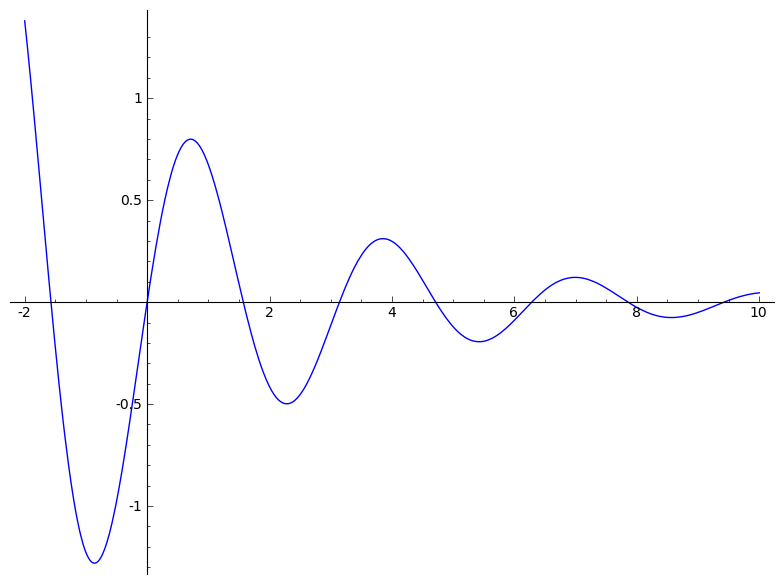
\includegraphics[scale=.1]{imagenes/mu_neg.png} & 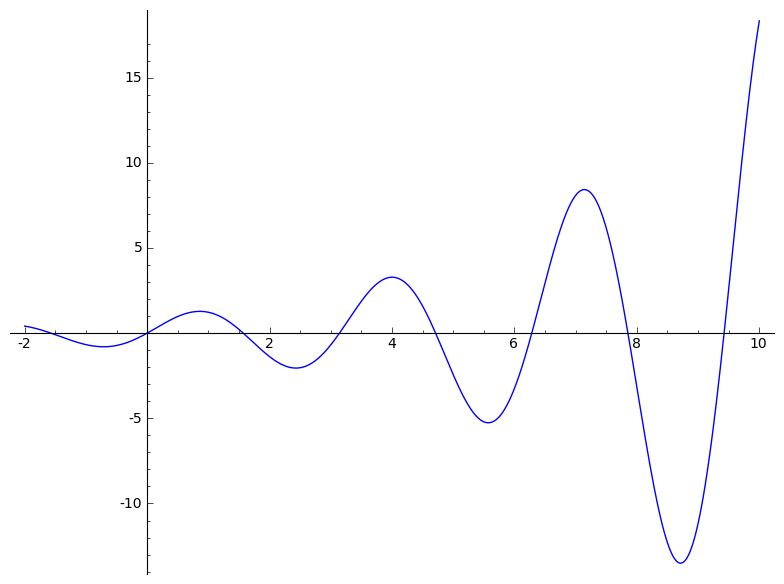
\includegraphics[scale=.1]{imagenes/mu_pos.png} &
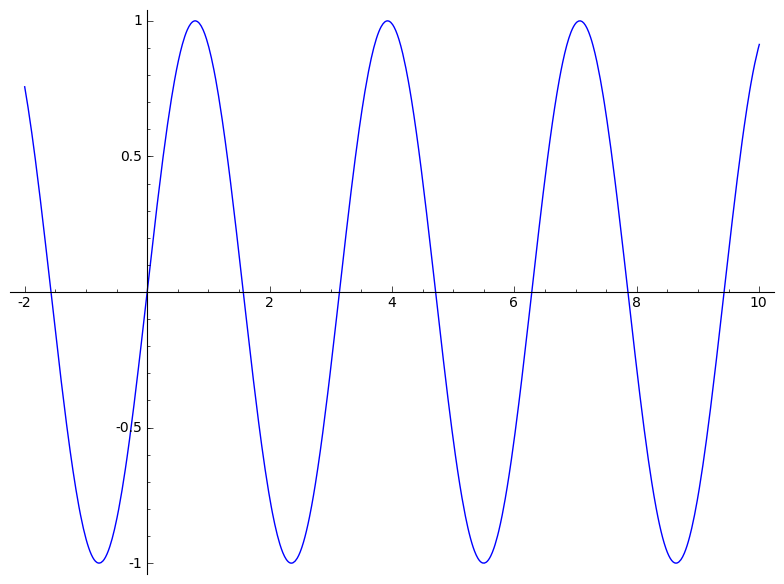
\includegraphics[scale=.1]{imagenes/mu_cero.png}\\
$\mu<0$ & $\mu>0$ & $\mu=0$\\
\end{tabular}

\end{center}








\item \noindent\textbf{ $\b{\Delta=p^2-4c=0}$, raices iguales }. Conocemos una soluci�n $\boxed{y_1=e^{-\frac{p}{2}x}}$. Podemos hallar otra
por el m�todo de reducci�n de orden. Esto consiste en proponer otra soluci�n de la forma $y_2(x)=y_1(x)v(x)$ Dejemos que lo haga \texttt{SymPy}


\begin{lstlisting}
>>> x,p=symbols('x,p')
>>> y=Function('y')(x)
>>> v=Function('v')(x)
>>> y=v*exp(-p/2*x)
>>> ecua=y.diff(x,2)+p*y.diff(x)+p**2/4*y
>>> ecuav=simplify(ecua/exp(-p/2*x))
>>> ecuav
\end{lstlisting}
Se obtiene
\[\frac{d^{2}}{d x^{2}}  v{\left (x \right )}=0.\]
La soluci�n general para $v$ es $v=c_1+c_2x$. As� el m�todo mencionado proporciona la soluci�n extra
\[\boxed{y_2(x)=xe^{-\frac{p}{2}x}}.\]
\end{enumerate}


\section{Ecuaci�n no homog�nea}
\subsection{M�todo coeficientes indeterminados}
Intentamos resolver
\boxedeq{\frac{d^2y}{dx^2}+p\frac{dy}{dx}+qy=r(x),}{ec_2_nohom}
donde $p,q,r \in \rr$, $r\in C(I)$ $r\neq 0$. El m�todo consiste en buscar soluciones en la misma clase de funciones a la que pertenece $r(x)$. Funciona de manera met�dica s�lo para algunos tipos de funciones $r(x)$.
Concretamente para $r(x)$ combinaci�n lineal de funciones polin�micas, exponenciales $e^{\alpha x}$ o trigonom�tricas $\cos \alpha x$ y $\sen \alpha x$.
Lo vamos a ilustrar con ejemplos para cada caso.



\begin{enumerate}
\item \textbf{Caso $\b{r(x)=e^{a x}}$ y $\b{a^2+pa+q\neq 0}$.}
En esta situaci�n se propone como soluci�n una funci�n de la forma $\boxed{y(x)=Ae^{ax}}$. Usamos \texttt{SymPy} para el c�lculo
\begin{lstlisting}
>>> x,p,q,a,A=symbols('x,p,q,a,A')
>>> y=A*exp(a*x)
>>> ecua=y.diff(x,2)+p*y.diff(x)+q*y-exp(a*x)
>>> ecua=simplify(ecua/exp(a*x))
>>> ecua
A*a**2 + A*a*p + A*q - 1
>>> solve(ecua,A)
[1/(a**2 + a*p + q)]
\end{lstlisting}


Si $a^2+pa+q\neq 0$, encontramos la soluci�n particular $\boxed{y(x)=\frac{1}{(a^2+pa+q)}e^{ax}}$.




\item \textbf{Caso $\b{r(x)=e^{a x}}$ y $\b{a^2+pa+q= 0}$.}
En esta situaci�n diremos que la ecuaci�n est� en \emph{resonancia}. M�s generalmente, diremos que se presenta resonancia cuando $r(x)$ es soluci�n
del problema homog�neo.
Propongamos como soluci�n $y(x)=Axe^{ax}$. Hagamos los c�lculos con \texttt{SymPy}.


\begin{lstlisting}
>>> x,p,q,a,A=symbols('x,p,q,a,A')
>>> y=A*x*exp(a*x)
>>> ecua=y.diff(x,2)+p*y.diff(x)+q*y-exp(a*x)
>>> ecua=simplify(ecua/exp(a*x))
>>> ecua
A*a*(a*x + 2) + A*p*(a*x + 1) + A*q*x - 1
>>> ecua.subs(q,-a**2 - a*p).simplify()
2*A*a + A*p - 1

\end{lstlisting}

Luego, si $2a+p\neq 0$, $\boxed{y(x)=\frac{1}{2a+p}xe^{ax}}$ resuelve el problema.





\item \textbf{Caso $\b{r(x)=e^{a x}}$, $\b{a^2+pa+q= 0}$ y $ \b{2a+p=0}$.}
Si $2a+p=0$, como tambi�n $a^2+pa+q=0$, tenemos que $a$ es una ra�z doble de la ecuaci�n $\lambda^2+p\lambda+q=0$.
En este caso, proponemos como soluci�n $y(x)=Ax^2e^{ax}$.

\begin{lstlisting}
>>> x,p,q,a,A=symbols('x,p,q,a,A')
>>> y=A*x**2*exp(a*x)
>>> ecua=y.diff(x,2)+p*y.diff(x)+q*y-exp(a*x)
>>> ecua=simplify(ecua/exp(a*x))
>>> ecua
A*p*x*(a*x + 2) + A*q*x**2 + A*(a**2*x**2 + 4*a*x + 2) - 1
>>> ecua.subs([(q,-a**2 - a*p) , (p,-2*a)]).simplify()
2*A - 1
\end{lstlisting}

Hay que tomar $\boxed{y(x)=\frac{1}{2}x^2e^{ax}}$







\item \textbf{Caso $\b{r(x)=\sen bx}$.}
Proponemos
\[y(x)=A\cos x+ B\sen x,\]
como candidato a soluci�n.
\begin{lstlisting}
>>> x,p,q,a,b,A,B=symbols('x,p,q,a,b,A,B')
>>> y=A*cos(b*x)+B*sin(b*x)
>>> ecua=y.diff(x,2)+p*y.diff(x)+q*y-sin(b*x)
>>> ecua.simplify()
-b**2*(A*cos(b*x) + B*sin(b*x)) - b*p*(A*sin(b*x) -
B*cos(b*x)) + q*(A*cos(b*x) + B*sin(b*x)) - sin(b*x)
\end{lstlisting}


La expresi�n en el miembro de la izquierda es una combinaci�n lineal de las funciones $\cos bx$ y $\sen bx$. Como estas funciones son linealmente independientes
debemos tener que los coeficientes en la combinaci�n lineal deben ser cero

\begin{lstlisting}
>>> ecua.expand().coeff(sin(b*x))
-A*b*p - B*b**2 + B*q - 1
>>> ecua.expand().coeff(cos(b*x))
-A*b**2 + A*q + B*b*p
\end{lstlisting}

Obtenemos un sistema de ecuaciones
\begin{equation}\label{sist_lin_1}
\left\{\begin{array}{l l}
-Abp - (b^2 - q)B & = 1\\
Bbp - (b^2 - q)A &=0
\end{array}
\right.
\end{equation}
%
Para que el sistema tenga soluci�n la matriz de coeficientes debe ser no singular
\[
0\neq\det \begin{pmatrix}
-bp & -(b^2-q)\\
-(b^2-q) & bp
\end{pmatrix} = -(b^2p^2+(b^2-q)^2)
\]
Podemos suponer $b\neq 0$, de lo contrario la ecuaci�n hubiese sido homog�nea. entonces la condici�n de arriba ocurre si y s�lo si
$p\neq 0$ o $b^2\neq q$. En esa situaci�n encontraremos una soluci�n de la forma
\[
\boxed{y(x)=A\cos bx + B\sen bx},
\]
donde $A$ y $B$ resuelven \eqref{sist_lin_1}.

\label{eq:forz_res}
Cuando $p=0$ y $b^2= q$ el sistema \eqref{sist_lin_1} puede no tener soluci�n. Notar que en este caso la ecuaci�n queda
\[
y''+b^2y=\sen bx
\]
Es una ecuaci�n de un oscilador arm�nico no homog�nea. Hab�amos visto que justamente $r(x)=\sen bx$ es una soluci�n del problema homog�no. Nuevamente
estamos en una situaci�n de resonancia. Como en casos anteriores hay que proponer como soluci�n
\[y(x)=x\left(A\cos x+ B\sen x\right),\]




\item \textbf{Caso $\b{r(x)=\sen bx}$ con resonancia}

\begin{lstlisting}
>>> x,b,A,B=symbols('x,b,A,B')
>>> y=x*(A*cos(b*x)+B*sin(b*x))
>>> ecua=y.diff(x,2)+b**2*y-sin(b*x)
>>> eq1=ecua.expand().coeff(sin(b*x))
>>> eq2=ecua.expand().coeff(cos(b*x))
>>> H=solve([eq1,eq2],[A,B])
>>> H
{B: 0, A: -1/(2*b)}
>>> y.subs(H)
-x*cos(b*x)/(2*b)
\end{lstlisting}



Encontramos la soluci�n general
\[\boxed{y(x)=-\frac{x}{2b}\cos bx}.\]
El caso donde $r(x)=\cos bx$ se trata de manera completamente similar.



\item \textbf{Caso $\b{r(x)}$ polinomio}
 Hay que proponer como soluci�n un polinomio, en primera instancia, del mismo grado.

 Supongamos

 \boxedeq{\frac{d^2y}{dx^2}+p\frac{dy}{dx}+q(x)y=c_0+c_1x+\cdots+c_nx^n}{eq:no_hom_pol}

Se propone $y=a_0+a_1x+\cdots+a_nx^n$. Luego

\[\begin{array}{l}
2a_2+3\cdot2x+\cdots+n(n-1)x^{n-2}+\\
pa_1+p2a_2x+\cdots+pna_nx^{n-1}+\\
qa_0+qa_1x+\cdots+qa_nx^n=c_0+c_1x+\cdots+c_nx^n
\end{array}
.\]

Como las funciones $1,x,\ldots,x^n$ son linealmente independientes, los coeficientes en ambos lados de la igualdad deben ser iguales.

\[
\begin{split}
2a_2+pa_1+qa_0&=c_0\\
3\cdot 2+2pa_2+qa_1&=c_1\\
 &\hspace{2mm} \vdots\\
n(n-1)+p(n-1)a_{n-1}+qa_{n-2} &=c_{n-2}\\
pna_{n}+qa_{n-1} &=c_{n-1}\\
qa_n &=c_n\\
\end{split}
\]
Es �til escribir estas igualdades matricialmente.
\[\begin{pmatrix} q &\cdots  &\cdots&\cdots&\cdots\\
&q & \cdots & \cdots&\cdots \\
\vdots & &\ddots&& \vdots\\
\vdots&&&q&pn\\
\vdots&&&&q\\
\end{pmatrix}
\begin{pmatrix}
a_0\\
a_1\\
a_2\\
\vdots\\
a_{n-1}\\
a_n
\end{pmatrix}
=
\begin{pmatrix}
c_0\\
c_1\\
c_2\\
\vdots\\
c_{n-1}\\
c_n
\end{pmatrix}
\]
Es un sistema tri�ngular superior que se resuelve por sustituci�n ascendente. Esto siempre que $q\neq 0$. En caso contrario la matr�z es singular y es posible que el sistema no tenga soluci�n.

El caso $q=0$ es una forma de resonancia. Puede ser tratado como las anteriores resonancias, pero notando que la ecuaci�n se reduce a $y''+py'=r$ conviene
tomar $v=y'$ como
nueva variable dependiente y reducir la ecuaci�n a una de primer orden.

\end{enumerate}

Por �ltimo se�alemos que si deseamos resolver un problema de la forma
\[L[y]\equiv y''+py'+qy=r_1(x)+\cdots +r_n(x),\]
donde las funciones $r_i$ son de alguna de las formas descriptas en los casos previos,
entonces la linealidad de $L$ implica que, si $y_i$
resuelve $L[y_i]=r_i$, $y=y_1+\cdots +y_n$ resuelve la ecuaci�n deseada.


\subsection{M�todo de variaci�n de los par�metros}

Queremos resolver la ecuaci�n
\begin{equation}\label{eq:2orden_gen}
y''(x)+p(x)y'(x)+q(x)y(x)=r(x).
\end{equation}
Supongamos que contamos con un par de soluciones $y_1$, $y_2$ linealmente independientes de la ecuaci�n homog�nea asociada
\begin{equation}\label{eq:hom_asoc}
y''(x)+p(x)y'(x)+q(x)y(x)=0.
\end{equation}
El m�todo de \href{http://en.wikipedia.org/wiki/Variation_of_parameters}{variacion de los par�metros} consiste en proponer una soluci�n de la forma
\boxedeq{y(x)=c_1(x)y_1(x)+c_2(x)y_2(x).}{eq:var_param0}
Hay dos funciones incognitas $c_1$ y $c_2$, pero s�lo una ecuaci�n. Tendremos 
por esto libertad de introducir otra condici�n que consideremos conveniente.
Tenemos
\[
y'=c_1'y_1+c_1y_1'+c_2'y_2+c_2y_2'.
\]
Pidamos que
\begin{equation}\label{eq:var_param1}
c_1'y_1+c_2'y_2=0.
\end{equation}
Supuesta esta igualad
\[ y'= c_1y_1'+c_2y_2'.\]
Derivando
\[ y''= c_1'y_1'+c_2'y_2'+c_1y_1''+c_2y_2''.\]
Entonces
\[
\begin{split}
r(x)&=y''+py'+qy\\
&=c_1'y_1'+c_2'y_2'+c_1y_1''+c_2y_2''+p(c_1y_1'+c_2y_2')+q(c_1y_1+c_2y_2)\\
&=c_1(y_1''+py_1'+qy_1)+c_2(y_2''+py_2'+qy_2)+c_1'y_1'+c_2y_2'\\
&=c_1'y_1'+c_2'y_2'
\end{split}
\]
Esta ecuaci�n junto a \eqref{eq:var_param1} nos dan el sistema
\boxedeq{
\left\{\begin{array}{c c}
c_1'y_1+c_2'y_2&=0\\
c_1'y_1'+c_2'y_2'&=r
\end{array}
\right.
}{eq:var_param_sis}
Las incognitas son $c_1'$ y $c_2'$. El determinante de la matriz de coeficientes es precisamente el Wronskiano $W$ de las soluciones $y_1$ e $y_2$, por la suposici�n
de independencia $W\neq 0$ y por lo tanto el sistema tiene soluci�n �nica.
Se tiene
\[c_1'=-\frac{\det\begin{pmatrix}
0 & y_2\\
r & y_2'
\end{pmatrix}
}{W}=-\frac{ry_2}{W}
\]
y
\[c_2'=-\frac{\det\begin{pmatrix}
y_1 & 0\\
y_1' & r
\end{pmatrix}
}{W}=\frac{ry_1}{W}
\]
En consecuencia
\boxedeq{c_1=-\int\frac{ry_2}{W}dx}{eq:c1}
y
\boxedeq{c_2=\int\frac{ry_1}{W}}{eq:c2}
Usando estas f�rmulas y \eqref{eq:var_param0} obtenemos una soluci�n particular del sistema. La soluci�n general es la suma de la particular m�s
una soluci�n general del homog�neo. Esta �ltima soluci�n general se escribe como una combinaci�n lineal gen�rica entre $y_1$ e $y_2$.

\begin{ejemplo} Resolver el siguiente pvi $y''+y=\csc x$, 
$y\left(\tfrac{\pi}{2}\right)=0$ y $y'\left(\tfrac{\pi}{2}\right)=1$. 
La ecuaci�n homog�nea asociada tiene el par $y_1(x)=\cos(x)$ e $y_1(x)=\sen(x)$ 
   de soluciones linealmente independientes.   El wronskiano es $W\equiv 1$ y 
entonces una soluci�n paarticular es
\[\begin{split}
  y(x)&=-\int \frac{ry_2}{W}dx y_1 +\int \frac{ry_1}{W}dx y_2\\
       &=-\int dx \cos(x)+\int \frac{1}{\tan(x)}dx \sen(x)\\
       &=-x\cos(x) +\ln(\sen(x))\sen(x).
 \end{split}
\]
 
 La soluci�n general es
 \[
  y(x)=-x\cos(x) +\ln(\sen(x))\sen(x)+c_1\cos(x)+c_2\sen(x).
  \]
Las condiciones $y\left(\tfrac{\pi}{2}\right)=0$ y 
$y'\left(\tfrac{\pi}{2}\right)=1$ nos conducen a $c_2=0$ y $c_1=\frac{\pi}{2}$.



\end{ejemplo}
\section{Conclusiones}

\begin{enumerate}
\item Si podemos encontrar dos soluciones linealmente independientes de una ecuaci�n lineal homog�nea de segundo orden, tenemos la soluci�n general a traves de
combinaciones lineales.
\item Si tenemos una soluci�n no trivial de una ecuaci�n lineal homog�nea de segundo orden podemos hallar otra por el m�todo de reducci�n de orden.
\item Podemos resolver completamente una ecuaci�n lineal homog�nea de segundo orden con coeficientes constantes.
\item Podemos resolver algunos problemas no homog�neos por el m�todo de coeficientes indeterminados.
\item Si conocemos las soluciones del problema homog�neo podemos resolver, en teor�a, el no homog�neno para cualquier $r(x)$ por el m�todo de variaci�n
de los par�metros
\end{enumerate}

\section{Aplicaciones}
\subsection{Vibraciones mec�nicas }
\begin{problema} Estudiar el movimiento de un resorte (c�mo el de la unidad 
anterior) pero suponer que adem�s de actuar sobre la masa la fuerza el�stica del 
resorte,
tenemos una fuerza de fricci�n debida a la resistencia del medio. Por la acci�n de esta fuerza, se dice que es un sistema resorte-masa amortiguado.
Adem�s suponemos que hay otra fuerza $F$ externa y que s�lo depende de $t$. Por ejemplo si el resorte se colocase verticalmente y se dejase suspendida
la masa, $F$ ser�a la fuerza de gravedad. Si la masa estuviese hecha de metal, $F$ podr�a ser una fuerza provista por un im�n. Por la acci�n de esta fuerza el sistema se
dice forzado. Por consiguiente el sistema completo, con la acci�n de las tres fuerzas, se denomina un sistema resorte-masa, amortiguado y forzado.
\end{problema}

La fuerza el�stica del resorte se modeliza con la Ley de Hooke.
Para la amortiguaci�n, supongamos que el m�dulo de la fuerza es proporcional a 
la velocidad de la masa. La constante de proporcionalidad $c$ se llama 
coeficiente de
\href{http://es.wikipedia.org/wiki/Viscosidad}{viscosidad}. La direcci�n y sentido de la fuerza amortiguadora es siempre contraria
al movimiento. Por el principio de conservaci�n de la energ�a, vemos que la fuerza de amortiguaci�n siempre realiza un trabajo $W$ negativo, por consiguiente
hace perder energ�a cin�tica. De la fuerza externa $F$ no sabemos nada en principio. Por todo lo expuesto, si ponemos un sistema
de coordenadas con origen en la posici�n de equilibrio del sistema masa-resorte y si $x(t)$ es la posici�n de la masa en el momento $t$, la ecuaci�n que gobierna
el sistema masa-resorte con amortiguaci�n y forzamiento es
\boxedeq{mx''(t)\underbrace{=}_\text{2� Ley Newton}\underbrace{-kx(t)}_
\text{Hooke}\underbrace{-cx'(t)}_\text{Amortiguaci�n}+\underbrace{F(t)}_\text{Fuerza externa}}{eq:res_amor_for}


\subsubsection{Vibraciones amortiguadas no forzadas ($c>0$, $F=0$) }

Escribamos la ecuaci�n \eqref{eq:res_amor_for} de la siguiente froma
\begin{equation}\label{eq:res_amor}
\boxed{x''(t)+2\mu x'(t)+\omega^2x=0}\quad 
\mu:=\frac{c}{2m},\omega:=\sqrt{\frac{k}{m}}.
\end{equation}
Las ra�ces de la ecuaci�n caracter�stica   son
\[
\boxed{\lambda_{1,2}=-\mu\pm\sqrt{\Delta},\quad \Delta:=\mu^2-\omega^2}
\]
\textbf{Caso $\Delta>0$.} Aqu� la viscocidad es ``grande'' relativa ala rigidez 
$k$. Se dice que el sistema est� sobreamortiguado.
En este caso tenemos dos soluciones
linealmente independientes del problema homog�neo y la soluci�n general de 
este es de la forma
\[x(t)=c_1e^{\lambda_1t}+c_2e^{\lambda_2t}\]
Notar que $\lambda_1,\lambda_2<0$. Supongamos que el sistema masa-resorte parte 
del resposo $x'(0)=0$ y de una posici�n indeterminada $x_0$. Resolvamos este pvi

\begin{lstlisting}
>>> from sympy import *
>>> init_printing()
>>> lambda1,lambda2,t,x0,c1,c2=symbols('lambda1,lambda2,t,x0,c1,c2')
>>> x=c1*exp(lambda1*t)+c2*exp(lambda2*t)
>>> C=solve([x.subs(t,0)-x0,x.diff(t).subs(t,0)], [c1,c2])
>>> C
\end{lstlisting}

\[\begin{Bmatrix}c_{1} : - \frac{\lambda_{2} x_{0}}{\lambda_{1} - 
\lambda_{2}}, & c_{2} : \frac{\lambda_{1} x_{0}}{\lambda_{1} - 
\lambda_{2}}\end{Bmatrix}\]

\begin{lstlisting}
>>> x=x.subs(C[0])
\end{lstlisting}
\boxedeq{
x(t)= x_0\left\{ \frac{\lambda_{1}
e^{\lambda_{2} t}}{\lambda_{1} - \lambda_{2}}-\frac{\lambda_{2} e^{\lambda_{1} t}}{\lambda_{1} - \lambda_{2}}\right\}
}{eq:sol_sub_amor}


\begin{lstlisting}
>>> x=x.subs({lambda1:-1,lambda2:-2,x0:1})
>>> plot(x,(t,0,10))
\end{lstlisting}


\begin{figure}[h]
\begin{center}
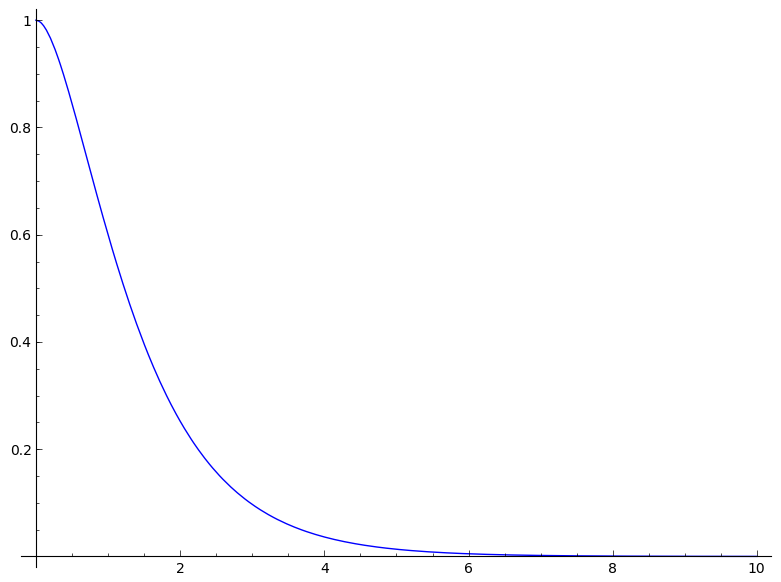
\includegraphics[scale=.2]{imagenes/sobreamortiguado.png}
\caption{ Vibraciones amortiguadas no forzadas ($c>0$, $F=0$) }\label{fig:VibrAmorNoFor}
\end{center}
\end{figure}



\begin{figure}[h]
\begin{center}
\animategraphics[controls, scale=.4]{15}{res_sobre/res_sobre-}{0}{60}
\vspace{.5cm}
\caption{Masa-resorte sobreamortiguado}\label{ani:VibrAmorNoFor}
\end{center}
\end{figure}

Como se observa en la gr�fica \ref{fig:VibrAmorNoFor} y la animaci�n \ref{ani:VibrAmorNoFor}
la masa ejecuta una oscilaci�n, lo cual le demanda un tiempo infinito. Podr�a 
haber pasado por la posici�n de equilibrio s�lo en el pasado, 
puesto que $x(t)=0$ cuando
\[\boxed{t=\frac{1}{\lambda_1-\lambda_2}\ln\frac{\lambda_1}{\lambda_2}<0}\]


\noindent\textbf{Caso $\Delta=0$.} En esta situaci�n se dice que hay amortiguaci�n cr�tica. Las ra�ces son iguales $\lambda_1=\lambda_2=-\mu$. Sabemos que
\boxedeq{x_1(t)=c_1e^{-\mu t}+c_2te^{-\mu t}=e^{-\mu t}\{c_1+c_2t\}}{eq:sol_gen_crit}
Nuevamente la soluci�n puede pasar a lo sumo una vez por la posici�n de equilibrio, siempre y cuando
$C_2\neq 0$. El compportamiento cualitativo de la soluci�n es muy parecido al caso anterior.


\noindent\textbf{Caso $\Delta<0$, caso subamortiguado.} $\lambda_{1,2}=-\mu\pm\nu i$ con $\nu=\sqrt{|\Delta|}=\sqrt{|\omega^2-\mu^2|}$.
La soluci�n general viene dada por
\boxedeq{x(t)=e^{-\mu t}\left\{ c_1\cos \nu t+c_2\sen \nu t \right\}}{eq:sol_gen_sub}
Est� funci�n tiene por gr�fica una onda sinusoidal modulada por una funci�n exponencial 
decreciente.

\begin{lstlisting}
sage: c1,c2,mu,nu,x0,t=var('c1,c2,mu,nu,x0,t')
sage: x=e^(-mu*t)*(c1*cos(nu*t)+c2*sin(nu*t))
sage: C=solve([x(t=0)==x0,x.diff(t).subs(t=0)==0],[c1,c2],solution_dict=True)
sage: x=x.subs(C[0]).subs({mu:.1,nu:4,x0:1})
sage: x.plot((x,0,100))
\end{lstlisting}
\begin{center}
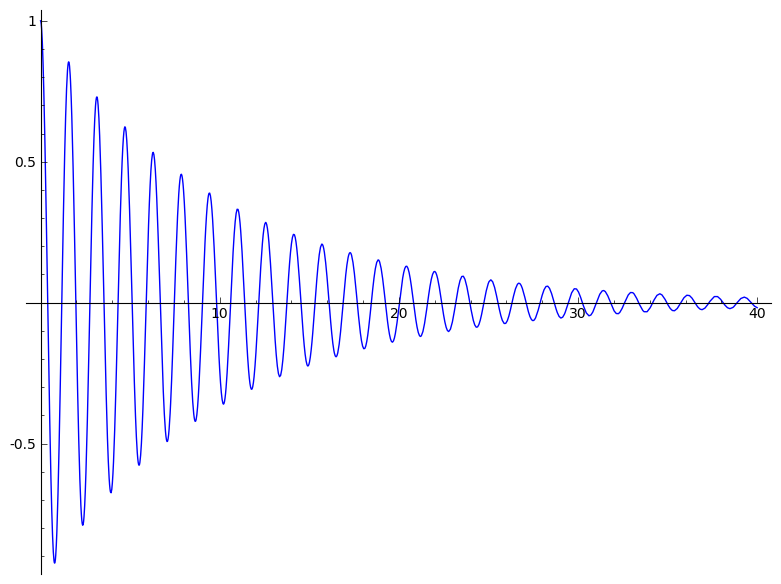
\includegraphics[scale=.15]{imagenes/subamortiguado.png}
\end{center}

{ Vibraciones amortiguadas no forzadas ($c>0$, $F=0$) }
\begin{figure}[h]
\animategraphics[controls, scale=.4]{15}{res_sub/res_sub-}{0}{60}
%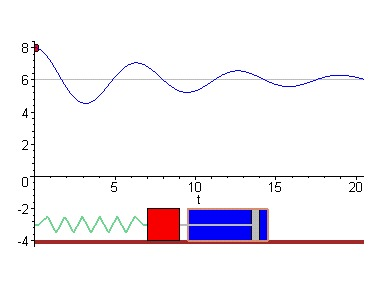
\includegraphics[scale=.4]{res_sub/res_sub-0.jpg}
\vspace{.5cm}
\caption{Masa-resorte subamortiguado}
\end{figure}

{ Vibraciones amortiguadas no forzadas ($c>0$, $F=0$) }
Se suele escribir la ecuaci�n \eqref{eq:sol_gen_sub} de otra forma. Expresemos el vector $(c_1,c_2)$ en
coordenadas polares.
\[
c_1=\rho\cos\alpha,\quad c_2=\rho\sen\alpha.
\]
Entonces
\[
x(t)=e^{-\mu t}\left\{ c_1\cos \nu t+c_2\sen \nu t \right\}=\boxed{\rho e^{-\mu t}\cos(\nu t-\alpha)}.
\]
Llamaremos este r�gimen \emph{movimiento cuasi-oscilatorio}. Se ejecutan vibraciones que se van amortiguando
de \href{http://es.wikipedia.org/wiki/Frecuencia}{frecuencia}
\[
f=\frac{1}{\text{per�odo}}=\frac{\nu}{2\pi},\quad \nu=\sqrt{\omega^2-\mu^2}=\sqrt{\left(\frac{k}{m}\right)^2-
\left(\frac{c}{2m}\right)^2}.
\]
En lugar de la frecuencia se suele considerar la
\href{http://luz.izt.uam.mx/mediawiki/index.php/Frecuencia_angular}{frecuencia angular} que se define como
$2\pi f$. La ventaja de esta definici�n es que la frecuencia �ngular de la funci�n de arriba es
$\nu$.

{ Vibraciones amortiguadas no forzadas ($c>0$, $F=0$) }
\textbf{Ejercicio:} En cualquiera de las situaciones descriptas, $x(t)\to 0$ y $x'(t)\to 0$, cuando $t\to\infty$.
Es decir, la masa se va deteniendo.

{ Vibraciones no amortiguadas y forzadas ($c=0$, $F\neq 0$) }
Vamos a considerar una fuerza externa oscilatoria de frecuencia angular $\omega_0$ y amplitud $F_0$. Tenemos que resolver
\boxedeq{x''(t)+\omega^2 x(t)=F_0\cos(\omega_0 t).}{eq:ecua_2orden_nohom}
Usaremos el m�todo de coeficientes indeterminados y SAGE. Antes, recordar que si $\omega=\omega_0$ estamos en
resonancia. Tendremos que considerar ese caso por separado. Supongamos pues $\omega\neq\omega_0$.
El siguiente c�digo se puede encontrar en la carpeta \texttt{scripts} del repositorio
\href{https://github.com/fdmazzone/Ecuaciones_Diferenciales}{GitHub} de esta materia. El script se denomina \texttt{osc\_arm\_forz\_noamort.sage}

% { Vibraciones no amortiguadas y forzadas ($c=0$, $F\neq 0$) }
% \lstinputlisting{scripts/osc_arm_forz_noamort.sage}
% Notar que el determinante del sistema de ecuaciones algebraicas es $-(\omega-\omega_0)^2$. Luego la matriz
% es no singular s�lo en no resonancia.
% La soluci�n general del problema es la soluci�n particular que acabamos de obtener m�s una soluci�n
% general del homog�neo que sabemos es una combinaci�n lineal generica entre $\cos \omega t$ y $\sin \omega t$.
%
% { Vibraciones no amortiguadas y forzadas ($c=0$, $F\neq 0$) }
% \boxedeq{x(t)=\frac{F_{0} \cos\left(\omega_{0} t\right)}{\omega^{2} - \omega_{0}^{2}}+
% c_1\cos(\omega t)+c_2\sin(\omega t).}{eq:sol_gen_noamort_forz}
% Como ya hemos visto, considerando las coordenadas polares $\rho$ y $\alpha$ de $c_1,c_2)$
% podemos reescribir la soluci�n
% \[x(t)=\frac{F_{0} \cos\left(\omega_{0} t\right)}{\omega^{2} - \omega_{0}^{2}}+
% \rho\cos(\omega t-\alpha)
% \]
% Vemos que el movimiento es la superposici�n de dos movimientos oscilatorios de frecuencias $\omega$, que se
% denomina la \emph{frecuencia natural} del resorte, y $\omega_0$ que se denomina \emph{frecuencia impresa}.
%
% \defverbatim[colored]\lstI{
% \begin{lstlisting}
% sage: t,omega,omega0,F0,rho,alpha=var('t,omega,omega0,F0,rho,alpha')
% sage: x=F0/(omega^2-omega0^2)*cos(omega0*t)+rho*cos(omega*t-alpha)
% sage: assume(-pi<alpha, alpha<2*pi)
% sage: solve([x(t=0)==0,x.diff(t).subs(t=0)==0],[rho,alpha])
% [omega*rho*sin(alpha) == 0, rho*cos(alpha) + F0/(omega^2 - omega0^2) == 0]
% sage: x0=x(alpha=0)
% sage: sol=solve([x0(t=0)==0,x0.diff(t).subs(t=0)==0],rho,\
% solution_dict=True)
% sage: x0=x0.subs(sol[0])
% sage: x0.factor().show()
% \end{lstlisting}
% }
% { Vibraciones no amortiguadas y forzadas ($c=0$, $F\neq 0$) }
% Resolvamos el pvi
% \[
% \left\{\begin{array}{l}
% x''(t)+\omega^2x(t)=F_0\cos(\omega_0 t),\\
% x'(0)=x(0)=0\\
% \end{array}
% \right.
% \]
% \lstI
% \[x(t)=-\frac{F_{0} \cos\left(\omega t\right)}{\omega^{2} - \omega_{0}^{2}} + \frac{F_{0} \cos\left(\omega_{0} t\right)}{\omega^{2} - \omega_{0}^{2}}
% \]
%
% \defverbatim[colored]\lstI{
% \begin{lstlisting}
% sage: x1=x0.subs({F0:1,omega:1,omega0:.9})
% sage: x1.plot(x,0,200)
% \end{lstlisting}
% }
% { Vibraciones no amortiguadas y forzadas ($c=0$, $F\neq 0$) }
% Ahora usemos la identidad $\cos(a-b)-cos(a+b)=2\sen a\sen b$, con $a=\frac12 (\omega+\omega_0)$ y
% $b=\frac12 (\omega-\omega_0)$. Deducimos
% \boxedeq{%
% x(t)=\frac{2F_{0} }{\omega^{2} - \omega_{0}^{2}}\sen (\omega-\omega_0)t \sen (\omega+\omega_0)t.
% }{eq:sol_gen_pulsos}
% Esta expresi�n la podemos ver como una onda de frecuencia grande $\omega+\omega_0$ modulada por una de frecuencia
% chica $\omega-\omega_0$.
% \lstI
% \begin{center}
% 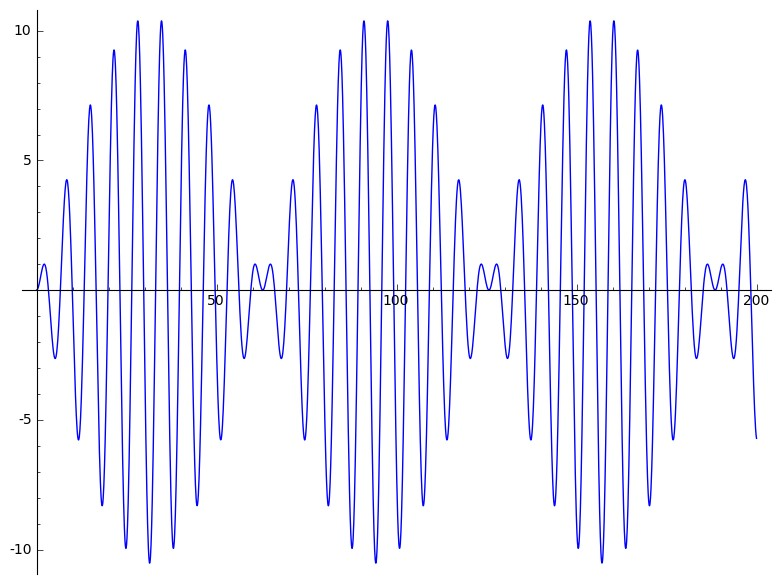
\includegraphics[scale=.15]{imagenes/batido.jpg}
% \end{center}
%
% \defverbatim[colored]\lstI{
% \begin{lstlisting}
% sage: limit(x0,omega0=omega)
% 1/2*F0*t*sin(omega*t)/omega
% \end{lstlisting}
% }
% { Vibraciones no amortiguadas y forzadas ($c>0$, $F\neq 0$) }
% Calculemos el l�mite $\lim_{\omega_0\to\omega}x(t)$,
% \lstI
% \[x(t)=\frac{F_{0} t \sin\left(\omega t\right)}{2 \, \omega}
% \]
% El caso $\omega=\omega_0$ es el caso con resonancia, que debemos resolver como fue indicado en la p�gina \ref{eq:forz_res},
% esto es proponiendo como soluci�n $y(x)=x\left(A\cos x+ B\sen x\right)$. El siguiente c�digo \texttt{SAGE} muestra que la soluci�n es la misma funci�n
% que la obtenida por el proceso de l�mite de los casos sin resonancia.
% \lstinputlisting{scripts/osc_arm_forz_noamort_res.sage}
%
% { Vibraciones no amortiguadas y forzadas ($c>0$, $F\neq 0$) }
% Se producen ``vibraciones'' no acotadas.
% \begin{center}
% 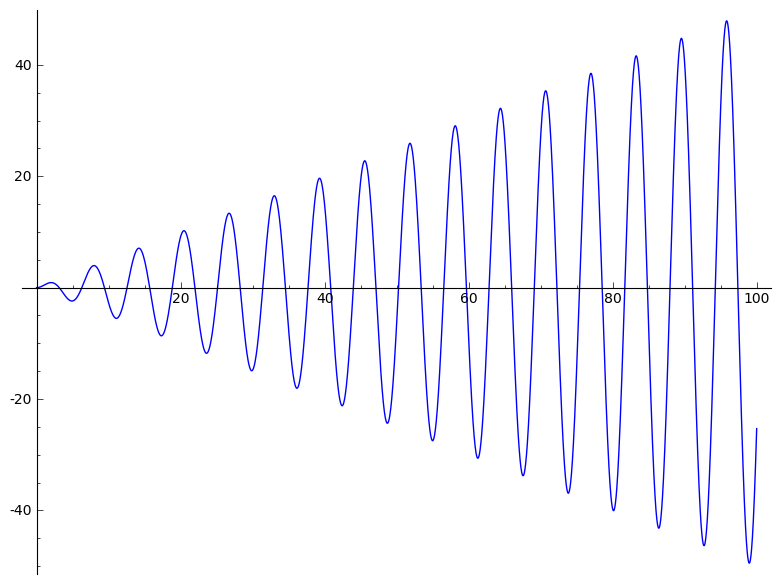
\includegraphics[scale=0.3]{imagenes/osc_arm_forz_res.png}
% \end{center}
% Ver la notebook \texttt{batido.sws}. En la wiki \href{http://wiki.sagemath.org/interact/misc\#Hearing_a_trigonometric_identity}{Hearing a trigonometric identity}
% se puede escuchar ondas sonoras con los fen�menos de resonancia y batido.
%
% { Vibraciones amortiguadas y forzadas ($c>0$, $F\neq 0$) }
% Vamos a considerar una fuerza externa oscilatoria de frecuencia $\omega_0$ y amplitud $F_0$. Tenemos que resolver
% \boxedeq{x''(t)+2\mu x'(t)+\omega^2 x(t)=F_0\cos(\omega_0 t).}{eq:ecua_2orden_amort_nohom}
% \lstinputlisting{scripts/osc_arm_forz_amort.sage}
%
% \defverbatim[colored]\lstI{
% \begin{lstlisting}
% sage: rho=sqrt(A**2+B**2).subs(SolAB[0]).simplify_full()
% sage: show(rho)
% \end{lstlisting}
% }
% { Vibraciones amortiguadas y forzadas ($c>0$, $F\neq 0$) }
% \boxedeq{x(t)=
% \frac{2 \, F_{0} \mu \omega_{0} \sin\left(\omega_{0} t\right)}{\omega^{4} + \omega_{0}^{4} + 2 \,
% {\left(2 \, \mu^{2} - \omega^{2}\right)} \omega_{0}^{2}} + \frac{{\left(F_{0} \omega^{2} -
% F_{0} \omega_{0}^{2}\right)} \cos\left(\omega_{0} t\right)}{\omega^{4} +
% \omega_{0}^{4} + 2 \, {\left(2 \, \mu^{2} - \omega^{2}\right)} \omega_{0}^{2}}
% }{eq:SolGennoHom}
% Es un movimiento oscilatorio de frecuencia angular $\omega_0$. Podemos escribir $x(t)=\rho\cos(\omega_0 t-\alpha)$,
% donde $(\rho,\alpha)$ son las coordenadas polares de $(A,B)$. En particular $\rho=\sqrt{A^2+B^2}$
% Recurrimos nuevamente a SAGE
% \lstI
% \[
% \rho(\omega_0)=\frac{F_{0}}{\sqrt{\omega^{4} + \omega_{0}^{4} + 2 \, {\left(2 \, \mu^{2} - \omega^{2}\right)} \omega_{0}^{2}}}=
% \frac{F_{0}}{\sqrt{(\omega^2-\omega_0^2)^2+4\mu^2\omega_0^2}}
% \]
%
% \defverbatim[colored]\lstI{
% \begin{lstlisting}
% sage: plot(rho.subs({F0:1, mu:.1,omega:5},(omega0,0,10) )
% \end{lstlisting}
% }
% { Vibraciones amortiguadas y forzadas ($c>0$, $F\neq 0$) }
% \[\alpha=\atan2\left( {{\omega^{2} -
% \omega_{0}^{2}} } , {2 \, \mu \omega_{0} } \right)
% \]
% En una consola de sage entrar \texttt{atan2?} para averiguar que funci�n es $\atan2$.
% Grafiquemos la funci�n $\rho(\omega_0)$ para $\omega=5$ y $\mu=0.1$.
% \lstI
% \begin{center}
% 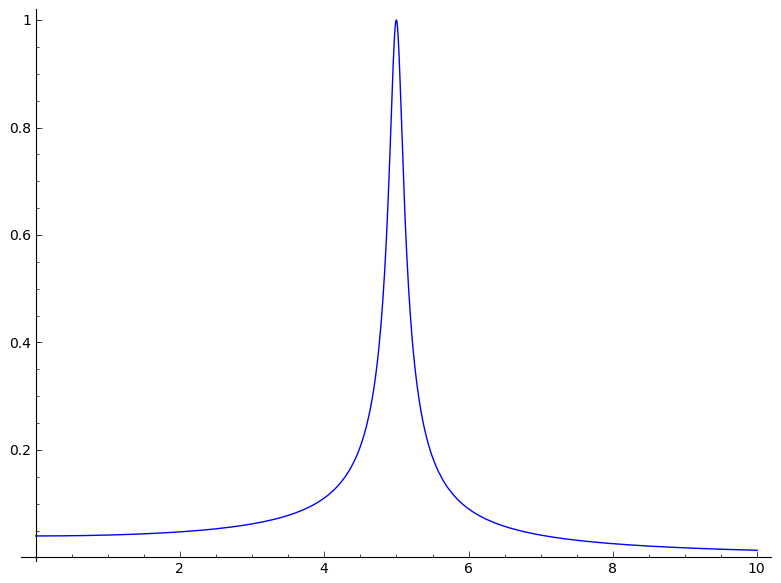
\includegraphics[scale=.2]{imagenes/rho_graf.png}
% \end{center}
%
% \defverbatim[colored]\lstI{
% \begin{lstlisting}
% sage: sol=solve(rho.diff(omega0),omega0)
% sage: sol
% [omega0 == -sqrt(-2*mu^2 + omega^2), omega0 == sqrt(-2*mu^2 + omega^2), omega0 == 0]
% sage: rho.diff(omega0,2).subs(sol[1]).simplify_full().show()
% \end{lstlisting}
% }
% \defverbatim[colored]\lstII{
% \begin{lstlisting}
% sage: sol[1].rhs().subs({mu:.1,omega:5})
% 4.99799959983992
% \end{lstlisting}
% }
% { Vibraciones amortiguadas y forzadas ($c>0$, $F\neq 0$) }
% La funci�n tiene un notorio m�ximo cerca de $\omega_0=5$. Seguramente es debido a la aparici�n de resonancias. Hallemos el punto de m�ximo exacto.
% \lstI
% Si $2\mu^2<\omega$ tendremos un m�ximo (en realidad un m�ximo local) en $\omega_{0} = \sqrt{-2 \, \mu^{2} + \omega^{2}}$. En el ejemplo que graficamos
% el m�ximo ocurre en
% \lstII
% Vale decir, un oscilador arm�nico en reposo es m�s sensible a exitaciones en ciertas frecuencias, aproximadamente la frecuencia
% natural del resorte cuando el coeficiente de viscocidad $c=2m\mu$ es chico. Esto es utilizado para dise�ar dispositivos que captan ondas s�smicas.
%
% { Vibraciones amortiguadas y forzadas ($c>0$, $F\neq 0$) }
% Hasta aqu� hemos encontrado una soluci�n particular del sistema no homog�neo. Para encontrar una soluci�n general deber�amos adicionar a la particular que disponemos
% una soluci�n general $x_g(t)$ de la ecuaci�n homog�nea. La forma de esta soluci�n general es de alguno de los tipos \ref{eq:sol_gen_sub},
% \ref{eq:sol_gen_crit} o \ref{eq:sol_sub_amor}. Sin embargo no nos importa ahora la f�rmula expl�cita de estas soluciones, sino que nos interesa resaltar que
% tr�tese del tipo que se trate, se satisface que $\lim_{t\to\infty}x_g(t)=0$. Por este motivo, vamos a decir que esta parte de la soluci�n es
% \emph{transitoria}. En cambio la soluci�n que prevalece en el tiempo dada por \eqref{eq:SolGennoHom} la denominaremos soluci�n \emph{estacionaria}.
%
% {Un poco de mec�nica celeste}
% Vamos a considerar ahora el problema del movimiento de un planeta, digamos la Tierra, de masa $m_{\earth}$ alrededor del sol de masa $m_{\sun}$. Como
% $m_{\sun}\gg m_{\earth}$ vamos a ignorar la fuerza que act�a sobre el Sol debido a la atracci�n gravitatoria de la Tierra. Esta suposici�n, aunque falsa, la hacemos
% por simplicidad. No obstante, con s�lo un poco de trabajo, el caso m�s general se reduce al tratado aqu�. Ver el trabajo final de la Lic. Matem�tica de Leopoldo Buri,
% para una deducci�n m�s cuidadosa. Vamos a suponer adem�s que el movimiento del planeta se retringe a un plano. Esta afirmaci�n es cierta y aunque su demostraci�n
% es sencilla no la desarrollaremos aqu�.
% Supongamos un sistema de coordenadas cartesianas sobre el plano en que se realiza el movimiento orbital del planeta. Asumimos el Sol en el origen de coordenadas y en
% reposo. Como no act�a fuerza sobre �l, permanecer� en esa situaci�n. Vamos a suponer que la posici�n de la Tierra es $\v{r}$.
%
% {Un poco de mec�nica celeste}
% Los dos ingredientes b�sicos para derivar la leyes de movimiento del planeta son la
% \href{http://es.wikipedia.org/wiki/Leyes_de_Newton\#Segunda_ley_de_Newton_o_ley_de_fuerza}{Segunda Ley de Newton} y la
% \href{http://es.wikipedia.org/wiki/Ley_de_gravitaci�n_universal}{Ley Gravitaci�n Universal}. Ya hemos considerado ambas con anterioridad.
% Seg�n la Ley de Gravitaci�n Universal, la magnitud de la fuerza de gravedad es proporcional a $\frac{m_{\earth}m_{\sun}}{d^2}$, donde $d$ es la distancia tierra-sol.
% A la constante de proporcionalidad la llamaremos, como es costumbre, $G$. La direcci�n de la fuerza gravitatoria es la de la recta que une los dos astros y
% el sentido es tal que la fuerza atrae los cuerpos. Vale decir, la direcci�n y sentido de la
% fuerza de gravedad vienen dados por el versor $-\v{r}/r$, donde $r=|\v{r}|$. Luego se debe satisfacer que
% \[Gm_{\earth}\frac{d^2\v{r}}{dt^2}=-\frac{Gm_{\earth}m_{\sun}}{r^2}\frac{\v{r}}{r}=-Gm_{\earth}m_{\sun}\frac{\v{r}}{r^3}. \]
%
% {Un poco de mec�nica celeste}
% Es decir
% \boxedeq{\frac{d^2\v{r}}{dt^2}=-\mu\frac{\v{r}}{r^3}\quad\text{donde } \mu:=Gm_{\sun}}{eq:grav}
% Esta ecuaci�n se conoce como la \href{http://es.wikipedia.org/wiki/Problema_de_los_dos_cuerpos}{ecuaci�n de los dos cuerpos}.
% Dado que esta ecuaci�n entra�a, a su vez, tres ecuaciones escalares, una por cada
% componente de $\v{r}$, se nos presenta aqu� un \emph{Sistema de Ecuaciones Diferenciales}. No sabemos resolver sistemas de ecuaciones. No obstante vamos
% a ver como podemos reducir la ecuaci�n anterior, mediante ingeniosos cambios de
% variables, a ecuaciones diferenciales que sabemos resolver.
%
% {Un poco de mec�nica celeste}
% Vamos a usar coordenadas polares $(r,\theta)$ y los versores $\v{u}_r:=(\cos\theta,\sen\theta)$ y $\v{u}_{\theta}:=(-\sen\theta, \cos\theta)$. Notar que
% $\v{u}_r \perp \v{u}_{\theta}$ y por consiguiente $\mathcal{B}:=\{\v{u}_r , \v{u}_{\theta}\}$ forma una base del espacio euclideano 2-dimensional. Usaremos este hecho
% para representar distintos vectores como combinaci�n lineal de vectores de la base. Los c�lculos, como es ya habitual, se los dejaremos a SAGE, pero esta vez
% usaremos \href{ http://www.sagemath.org/doc/tutorial/sagetex.html}{\textsf{Sage\TeX}} como interfaz de SAGE.
% \textsf{Sage\TeX} permite incrustar c�digo y outputs de SAGE dentro de un archivo \LaTeX .
% Todos los c�lculos que realizamos los pueden encontrar en el script \texttt{2cuerpos.sage} dentro de la carpeta scripts en
% el repositorio de \href{https://github.com/fdmazzone/Ecuaciones_Diferenciales}{GitHub}
% que mantiene materiales de este curso. Ver el siguiente enlace
% \href{https://github.com/fdmazzone/Ecuaciones_Diferenciales}{https//github.com/fdmazzone/Ecuaciones\_Diferenciales}
%
% {Un poco de mec�nica celeste}
% Primero declaramos las variables y asignamos los vectores $\v{u}_r$, $\v{u}_{\theta}$ y el vector
% $\v{r}$ al que llamamos \texttt{pos}.
%
% t,mu=var('t,mu')
% x=function('x',t)
% y=function('y',t)
% r=function('r',t)
% theta=function('theta',t)
% u_r=vector([cos(theta),sin(theta)])
% u_theta=vector([-sin(theta),cos(theta)])
% pos=(r*u_r).column()
%
% Como vamos a necesitar representar vectores en la base $\mathcal{B}=\{\v{u}_r , \v{u}_{\theta}\}$, constru�mos una matriz
% con los vectores de la base en las columnas.
%
% M=matrix([[cos(theta),-sin(theta)],\
% [sin(theta),cos(theta)]])
%
%
% {Un poco de mec�nica celeste}
% Demosle un vistazo a $M$
% \[M:=\sage{M}.\]
% Concretamente queremos representar el vector aceleraci�n $\v{a}:=\tfrac{d^2\v{r}}{dt^2}$ en la base $\mathcal{B}$, para ello debemos resolver $MX=\v{a}$, donde $X$ y
% $\v{a}$ los asumimos vectores columna. Con SAGE lo hacemos en un periquete
%
% sol=M.solve_right(pos.derivative(t,2))
% a1=sol[0].simplify_full()
% a2=sol[1].simplify_full()
%
% Obtenemos asi las dos componetes de $\v{a}$.
%
% {Un poco de mec�nica celeste}
% En la notaci�n de SAGE
% \[
% \v{a}=\left(\begin{array}{c}
% \sage{a1}\\
% \sage{a2}
% \end{array}
% \right)
% \]
% En la que nos gusta m�s
% \[
% \v{a}=\left(\begin{array}{c}
% \ddot{r}-r\dot{\theta}^2 \\
% r\ddot{\theta}+2\dot{r}\dot{\theta}
% \end{array}
% \right)=
% \left(\begin{array}{c}
% \ddot{r}-r\dot{\theta}^2 \\
% \frac{1}{r}\frac{d}{dt} \left( r^2\dot{\theta} \right)
% \end{array}
% \right)
% \]
%
% {Un poco de mec�nica celeste}
% El vector aceleraci�n debe ser igual a la fuerza por unidad de masa $-\mu \v{r}/r^3$. Notemos que esta fuerza es
% \href{http://es.wikipedia.org/wiki/Campo_central}{central}, es decir tiene componente nula
% respecto al vector $\v{u}_{\theta}$. Por consiguiente se debe satisfacer que
% \[\frac{1}{r}\frac{d}{dt} \left( r^2\dot{\theta} \right)=0\Longleftrightarrow \exists h\in\mathbb{R}: \boxed{ r^2\dot{\theta}=h}. \]
% \begin{tabular}{m{5cm} m{5cm}}
% Hemos derivado la \href{http://es.wikipedia.org/wiki/Leyes_de_Kepler}{Segunda Ley de Kepler}: El radio vector barre �reas iguales en tiempos iguales.
% &
% 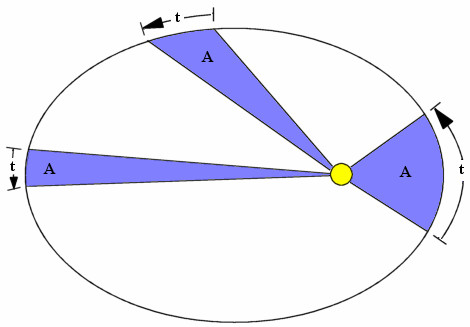
\includegraphics[scale=.3]{imagenes/2leykepler.jpeg}\\
% \end{tabular}
%
% {Un poco de mec�nica celeste}
% En la direcci�n radial $\v{u}_r$ la componente de la fuerza es $-\mu/r^2$. Es decir se satisface la ecuaci�n
% \[
% \ddot{r}-r\dot{\theta}^2=-\frac{\mu}{r^2}
% \]
% Notar que esta ecuaci�n entra�a dos incognitas $r$ y $\theta$, pero $\dot{\theta}$ puede ser remplazado por $h/r^2$ por la segunda Ley de Kepler.
% Declaremos la variable $h$ que juega un rol importante y reemplacemos $\dot{\theta}$ en la ecuaci�n
%
% h=var('h')
% ed=(a1[0]).subs_expr(theta.diff(t)==h/r^2)
% ed+=mu/r^2
%
% Resulta
% \[\sage{ed}\]
%
% {Un poco de mec�nica celeste}
% Conseguimos una ecuaci�n no lineal de segundo orden para $r$. De los m�todos que hemos visto, ninguno se aplica a esta ecuaci�n.
% El truco m�gico consiste en considerar la nueva variable dependiente $z=1/r$ y la nueva variable independiente
% $\theta$.
%
% z=function('z',theta)
% r=1/z
% ed2=r.diff(t,2)+mu/r^2-h^2/r^3
%
% Se obtiene
% \begin{sagecommandline}
% sage: ed2
% -h^2*z(theta(t))^3 + mu*z(theta(t))^2 +
% ...2*D[0](theta)(t)^2*D[0](z)(theta(t))^2/z(theta(t))^3 -
% ...D[0](theta)(t)^2*D[0, 0](z)(theta(t))/z(theta(t))^2
% ...- D[0, 0](theta)(t)*D[0](z)(theta(t))/z(theta(t))^2
% \end{sagecommandline}
%
% {Un poco de mec�nica celeste}
% En la ecuaci�n resultante, nuevamente aparece $\dot{\theta}$ y adem�s ahora aparece $\ddot{\theta}$. Tenemos que reemplazar
% $\dot{\theta}$ por $hz^2$ y $\ddot{\theta}$ por $\tfrac{d}{dt}hz^2$.
%
% theta2diff=(h*z^2).diff(t).\
% subs_expr(theta.diff(t)==h*z^2)
% ed3=ed2.subs_expr\
% (theta.diff(t)==h*z^2,theta.diff(t,2)==theta2diff)
% ed4=(ed3/z^2/h^2).expand()
%
% Resulta
% \[\sage{ed4}\]
% La ecuaci�n del oscilador arm�nico. Sabemos resolver esta ecuaci�n y SAGE tambi�n!!
%
% s=var('s')
% ed5=ed4.subs_expr(theta==s)
% sol1=desolve(ed5,z,ivar=s)
%
%
% {Un poco de mec�nica celeste}
% obtenemos
% \[
% \sage{sol1}
% \]
% Ahora si escribimos $k_1=\rho\cos\omega$ y $k_2=-\rho\sen\omega$ y recordamos que $z=1/r$, deducimos
% \[r=\frac{1}{\frac{\mu}{h^2}+\rho\sen(s-\omega)}\]
% Llamando $p=\tfrac{h^2}{\mu}$ y $e=\tfrac{\rho h^2}{\mu}$
% \boxedeq{r=\frac{p}{1+e\sen(s-\omega)}}{eq:orb_elipse}
%
% {Un poco de mec�nica celeste}
% \textbf{Ejercicio:} La ecuaci�n \eqref{eq:orb_elipse} es la ecuaci�n de una c�nica con foco en el origen y excentricidad $e$.
% Recordemos que la variable $s$ es el �ngulo polar.
% Hagamos algunos gr�ficos
%
% ListaGra=plot([])
% for e in srange(0,.8,.1):
%     ListaGra+=polar_plot(1/(1+e*cos(s)),\
% (s,0,2*pi),rgbcolor=(e,1-e,0))
%     ListaGra+=polar_plot(1/(1+cos(s)),\
% (s,-3*pi/4,3/4*pi),rgbcolor=(e,1-e,0))
% for e in srange(1.2,2,.1):
%     ListaGra+=polar_plot(1/(1+e*cos(s)),\
% (s,-0.65*pi,0.65*pi),rgbcolor=(0,2-e,e-1))
% gra=ListaGra.show()
%
%
% {Un poco de mec�nica celeste}
% \begin{center}
% 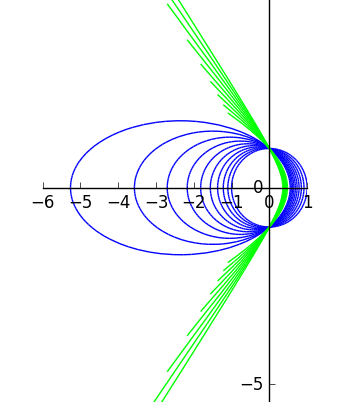
\includegraphics[scale=.5]{imagenes/conicas.png}
% \end{center}
%
% {Un poco de mec�nica celeste}
% Hemos logrado encontrar $r$ como funci�n de $\theta$. No obstante
% no hemos logrado resolver a�n el problema de los dos cuerpos \eqref{eq:grav}, para ello deber�amos encontrar $\v{r}(t)$, es decir poner a $
% \v{r}$ como funci�n de $t$. Esto nos servir�a para decir que punto de la �rbita ocupa el planeta en un dado momento. Este problema no lo desarrollaremos aqu� dado
% que su soluci�n se aparta del tema de las ecuaciones diferenciales.
%




\end{document}
% 
\chapter{Ecuaciones lineales de segundo orden}
%\author{Fernando Mazzone}


\section{Teorema de separación de Sturm}
\subsection{Motivación}


El objetivo  de esta unidad es mostrar como se pueden estudiar propiedades de las soluciones de ecuaciones lineales de segundo orden sin resolver la ecuación diferencial. En particular estudiaremos propiedades de  los \href{http://es.wikipedia.org/wiki/Raíz_de_una_función}{ceros} de las soluciones. Recordemos que denominamos cero de una función $y$ a un punto $x$ tal que $y(x)=0$.

Veamos como se comportan los ceros de la ecuación $y''+ay=0$. Para ser más concretos consideremos el siguiente pvi asociado a esta ecuación.
\[\left\{\begin{array}{l}
    y''+ay=0.\\
    y(0)=0,\quad y'(0)=1\\
  \end{array}\right.
  \]
Las soluciones  acordes al valor de $a$ son
\[
y(x)=\left\{\begin{array}{l l}
    \frac{1}{2\sqrt{|a|}}e^{\sqrt{|a|}x}- \frac{1}{2\sqrt{|a|}}e^{-\sqrt{|a|}x} &\text{cuando } a<0\\
     x &\text{cuando } a=0\\
     \frac{1}{\sqrt{|a|}}\sen(\sqrt{a}x) &\text{cuando } a>0\\
\end{array}\right..
\]
En la siguiente animación representamos los gráficos de las soluciones a medida que $a$ varía desde $-2$ hasta $6$ de a saltos de $0.1$.  
\begin{center}
\animategraphics[controls, scale=.4]{15}{ondas/ondas}{0}{79}
\end{center}
La separación entre ceros sucesivos de la  solución disminuye a medida que $a$ crece, la solución pasa de tener un único cero para $a<0$  a tener, cuando $a>0$, infinitos separados una distancia de $\pi/\sqrt{a}$. Cuando $a>0$, el número $\sqrt{a}$ es la frecuencia circular  de la solución sinusoidal $y(x)=   \frac{1}{\sqrt{|a|}}\sen(\sqrt{a}x)$, por analogía la seguiremos denominando frecuencia para otros valores de $a$.

Vamos a desarrollar dos resultados principales, el Teorema de Separación de Sturm y el Teorema de Comparación de Sturm. Luego generalizaremos este último teorema al Teorema de Comparación de Sturm-Picone.

\subsection{Teorema separación de Sturm}

Nuestra investigación sobre los ceros de soluciones comienza con el siguiente teorema que muestra que los ceros de soluciones linealmente independientes alternan entre si.




\begin{teorema}[\href{http://en.wikipedia.org/wiki/Sturm_separation_theorem}{Separación de Sturm}]{sep_sturm} Sean $y_1$ e $y_2$ soluciones linealmente independientes de 
\boxedeq{y''+P(x)y'+Q(x)y=0.}{eq:2_orden_hom}
Entonces entre dos ceros consecutivos de $y_2$ hay exactamente un cero de $y_1$. \end{teorema}
\begin{demo} Sean $x_1$ y $x_2$ ceros sucesivos de $y_2$. Podemos suponer $y_2>0$ en $(x_1,x_2)$. Vamos a considerar el Wronskiano de las soluciones
\[W=y_1(x)y_2'(x)-y_2(x)y_1'(x),\]
que es no nulo por la independencia lineal y por lo tanto tiene siempre el  mismo signo. En los puntos $x_1$ y $x_2$ tenemos $W=y_1(x)y_2'(x)$. Notar que
\[y_2'(x_1)=\lim_{h\to 0+}\frac{y_2(x_1+h)}{h}\geq 0.\]
De  manera similar deducimos $y_2'(x_2)\leq 0$. Por la invariancia del signo de $W=y_1y_2'$ debe ocurrir que $y_1(x_1)$ e $y_1(x_2)$ tienen signos diferentes. Y por lo tanto $y_1$ se debe anular en $(x_1,x_2)$.\end{demo}

\begin{ejemplo} Las funciones $y_1(x)=c_1\cos x+c_2\sen x$ e $y_2(x)=c_3\cos x+c_4\sen x$ son soluciones de la ecuación del oscilador armónico $y''+y=0$. Para que sean linealmente independientes se tiene que satisfacer que el Wronskiano $W$ sea no nulo en todo punto. Evaluamos $W$  en $0$ 
\[W=\det\begin{pmatrix} y_1(0) & y_2(0)\\y_1'(0) & y_2'(0) 
\end{pmatrix}=\det\begin{pmatrix} c_1 & c_3\\c_2 & c_4 
\end{pmatrix}=c_1c_4-c_2c_3\neq 0\]
Bajo este supuesto los ceros de $y_1$ e $y_2$ alternan. Veamos esta afirmación de manera directa, sin invocar el Teorema de Separación de Sturm. Como  es costumbre escribamos 
\[\begin{split}
y_1(x)=\rho_1\cos(x-\alpha_1),&\quad\text{donde } c_1=\rho_1\cos\alpha_1\text{ y }c_2=\rho_1\sen\alpha_1\\
y_2(x)=\rho_2\cos(x-\alpha_2),&\quad\text{donde }c_3=\rho_2\cos\alpha_2\text{ y }c_4=\rho_2\sen\alpha_2.
\end{split}
\]
La condición $c_1c_4-c_2c_3\neq 0$ equivale a la independencia lineal de los vectores $(c_1,c_2)$ y $(c_3,c_4)$ y esto último a que $\alpha_1-\alpha_2\notin\mathbb{Z}$. Por consiguiente los ceros de $y_1$ e $y_2$ alternaran como predice el Teorema. 


\end{ejemplo}

\subsection{Reducción a la ecuación normal}

La ecuación general lineal  de segundo orden  \eqref{eq:2_orden_hom} no es muy apropiada para el estudio que nos proponemos. Vamos a mostrar que podemos reducir aquella ecuación a una más simple que denominaremos \emph{normal}.

\begin{teorema} Existe una función $v$ tal que el cambio de variables $y(x)=v(x)u(x)$ transforma la ecuación \eqref{eq:2_orden_hom} en la ecuación
\boxedeq{u''+q(x)u=0.}{eq:2_orden_hom_can}
\end{teorema}
\begin{demo} 
\begin{lstlisting}
>>> from sympy import *
>>> init_printing()
>>> x=var('x')
>>> u,v,P,Q=symbols('u v P Q',cls=Function)
>>> y=u(x)*v(x)
>>> eq=y.diff(x,2)+P(x)*y.diff(x)+Q(x)*y
>>> eq.expand().coeff(u(x).diff(x))
P(x)*v(x) + 2*Derivative(v(x), x)
\end{lstlisting}

Para que la ecuación lineal de segundo orden resultante no tenga el término con $u'$ se debe cumplir que
\[ P{\left (x \right )} v{\left (x \right )} + 2 \frac{d}{d x} v{\left (x \right )}=0,\]
que es una ecuación lineal de primer orden para $v$, cuya  solución general es $v(x)=e^{-\int\frac{P}{2}dx}$.
\end{demo}

Hallemos $q$.
\begin{lstlisting}
>>> y=u(x)*exp(-Integral(P(x)/2,x))
>>> eq=y.diff(x,2)+P(x)*y.diff(x)+Q(x)*y
>>> eq=eq/exp(-Integral(P(x)/2,x))
>>>  eq.simplify()
\end{lstlisting}


Obtenemos
\[\boxed{- \frac{1}{4} P^{2}{\left (x \right )} u{\left (x \right )} + Q{\left (x \right 
)} u{\left (x \right )} - \frac{1}{2} u{\left (x \right )} \frac{d}{d x} P{\left
 (x \right )} + \frac{d^{2}}{d x^{2}}  u{\left (x \right )}=0}.\]
y por lo tanto
\[\boxed{q=- \frac{1}{4} P^{2}{\left (x \right )} + Q{\left (x \right )} - \frac{1}{2} \frac{d}{d x} P{\left (x \right )}}.\]
 
\begin{ejemplo} Un caso particular de importancia lo constituye la ecuación de Bessel
 \boxedeq{x^2y''+xy'+(x^2-a^2)y=0}{bessel}.
La ecuación equivale a
\begin{equation}\label{bessel_normal}\boxed{u''+\left(1+\frac{1-4a^2}{4x^2}\right)u=0}.
\end{equation}
\end{ejemplo}

Notar que si $v(x)\neq 0$, entonces los ceros de la función $u(x)$ e $y(x)=v(x)u(x)$ son los mismos. De allí que, si nuestro objetivo es estudiar ceros de soluciones de ecuaciones lineales de segundo orden, podemos suponer que la ecuación viene dada en la forma normal  \eqref{eq:2_orden_hom_can}.

Por  analogía  entre las ecuación a coeficientes constantes $y''+ay=0$ y la ecuación con coeficientes variables \eqref{eq:2_orden_hom_can}, llamaremos a la función $q(x)$ frecuencia. El objetivo que tenemos es ver si se observa un comportamiento similar entre las soluciones de la ecuación  \eqref{eq:2_orden_hom_can} y las de su contraparte a coeficientes constantes. 

\subsection{Teorema de Comparación de Sturm}

\begin{teorema} Sean $q_i$, $i=1,2$,  continuas e  $y_i$, $i=1,2$, soluciones de
\[ y_i''(x)+q_i(x)y_i(x)=0,\quad i=1,2.\]
Sean $x_0$ y $x_1$ ceros sucesivos de $y_2$ y supongamos que $q_2(x)\leq q_1(x)$ y $q_2\not\equiv q_1$ en $[x_0,x_1]$. entonces $y_1$ tiene al menos un cero en $(x_0,x_1)$. 
\end{teorema}
\begin{demo} Por la linealidad de las ecuaciones y como $x_0$ y $x_1$ son ceros consecutivos, podemos suponer $y_2>0$ en $(x_0,x_1)$. Supongamos que $y_1$ no tiene ceros en $(x_0,x_1)$, entonces en virtud del \href{http://es.wikipedia.org/wiki/Teorema_del_valor_intermedio}{Teorema de Bolzano}, $y_1$ no cambia de signo en $(x_0,x_1)$ y por consiguiente podemos suponer también que $y_1>0$ en $(x_0,x_1)$. Derivando el Wronskiano y usando las ecuaciones diferenciales que satisfacen $y_1$ e $y_2$ 
\[\begin{split}
\frac{dW}{dx} &= \frac{d}{dx} (y_1y_2'-y_1'y_2)\\
&=y_1y_2''-y_1''y_2\\
&=-q_2y_1y_2+q_1y_1y_2\\
&=(q_1-q_2)y_1y_2\geq 0\\
\end{split}
\]
Integrado esta desigualdad, tomando en cuenta que $q_1\not\equiv q_2$ y que $x_0$ y $x_1$ son ceros de $y_2$
\begin{equation}\label{wro_cre}0<\int_{x_0}^{x_1}\frac{dW}{dx}dx=W(x_1)-W(x_2)=y_1(x_1)y_2'(x_1)-y_1(x_0)y_2'(x_0).
\end{equation}
Por un razonamiento análogo al de la demostración del Teorema \ref{sep_sturm} debemos tener que $y_2'(x_0)\geq 0$ e $y_2'(x_1)\leq 0$. Luego $y_1(x_0)y_2'(x_0)\geq 0\geq y_1(x_1)y_2'(x_1)$ que es una contradicción con \eqref{wro_cre}.\end{demo}


\begin{corolario} Si $q\leq 0$ y $q\not\equiv 0$ en el intervalo, acotado o no, $I$ e  $y(x)$ es solución de $y''+q(x)y=0$, entonces $y$ tiene a los sumo un cero en $I$.
\end{corolario}
\begin{demo} Si $y(x)$ tuviese dos ceros entonces podemos usar el Teorema de Comparación de Sturm con $q_2=q$, $y_2=y$, $q_1=0$ e $y_1\equiv 1$ (notar que $y_1$ resueleve $z''+q_1(x)z=0$) y llegaríamos a que $y_1$ debería anularse en algún punto. Esta contradicción demuestra el corolario.  
\end{demo}



\begin{corolario} Si existe $q_0\in\mathbb{R}$ tal que  $q(x)\geq q_0>0$ en $I=(a,+\infty)$ y si  $y(x)$ es solución de $y''+q(x)y=0$, entonces $y$ tiene infinitos ceros en el intervalo no acotado $(a,+\infty)$. De hecho $y$ tiene un cero en cualquier intervalo de longitud $\pi/\sqrt{q_0}$.
\end{corolario}
\begin{demo}  Evidentemente hay que usar el Teorema de Comparación de Sturm con la ecuación $z''+q_0z=0$. La función  $z(x)=\cos(\sqrt{q_0}x-\alpha)$ es solución  esta ecuación. La función $z$ tiene ceros en  $k\frac{\pi}{\sqrt{q_0}}+\alpha$, $k=1,2,\ldots$. Si $[a,b]$ es cualquier intervalo de longitud $ \frac{\pi}{\sqrt{q_0}}$, podemos elegir $\alpha=a$ y entonces $b$ será $\frac{\pi}{\sqrt{q_0}}+\alpha$. Por consiguiente $y$ tiene un cero en $[a,b]$.
\end{demo}



\begin{corolario} Supongamos que $q(x)\geq (1+\epsilon)/4x^2$, para $x>0$. Entonces toda solución de 
$y''+q(x)y=0$ tiene infinitos ceros en $(0,+\infty)$. Más aún, hay una sucesión de ceros tendiendo a infinito y otra tendiendo a cero.
\end{corolario}

\begin{demo} En la ecuación 
\begin{equation}\label{eq_osc}\frac{d^2z}{dx^2}+\frac{1+\epsilon}{4x^2}z=0,
\end{equation}
hagamos el cambio de variable dependiente $z=y\sqrt{x}$. Primero computemos las derivadas
\[
\frac{dz}{dx}=\frac{x^{-\frac{1}{2}}}{2}y+x^{\frac{1}{2}}\frac{dy}{dx}
\]
y
\begin{equation}\label{sus_1}
\frac{d^2z}{dx^2}=-\frac{x^{-\frac{3}{2}}}{4}y+ x^{-\frac{1}{2}}\frac{dy}{dx} +x^{\frac{1}{2}}\frac{d^2y}{dx^2}
\end{equation}
Sustituyendo \eqref{sus_1} y  $z=y\sqrt{x}$ en \eqref{eq_osc} obtenemos
\begin{equation}\label{eq_osc2}
\begin{split}
 0&=\frac{d^2z}{dx^2}+\frac{1+\epsilon}{4x^2}z\\
 &=-\frac{x^{-\frac{3}{2}}}{4}y+
x^{-\frac{1}{2}}\frac{dy}{dx} +x^{\frac{1}{2}}\frac{d^2y}{dx^2}+\frac{1+\epsilon}{4x^2}
x^{\frac{1}{2}}y\\
&=\boxed{\frac{\epsilon}{4}x^{-\frac{3}{2}}y+ x^{-\frac{1}{2}}\frac{dy}{dx} +x^{\frac{1}{2}}\frac{d^2y}{dx^2}}.
\end{split}
\end{equation}
Ahora cambiemos la variable independiente por $t=\ln x$. Entonces
\begin{equation}\label{sus_2}\frac{dy}{dx}=\frac{dy}{dt}\frac{dt}{dx}=\frac{1}{x}\frac{dy}{dt}=\boxed{
e^{-t}\frac{dy}{dt}}.
\end{equation}
y
\begin{equation}\label{sus_3}
\begin{split}
\frac{d^2y}{dx^2}&=\left(\frac{d}{dx}e^{-t}\right)\frac{dy}{dt}+
e^{-t}\frac{d}{dx}\left(\frac{dy}{dt}\right)\\
&=e^{-t}\left(\frac{-1}{x}\right)\frac{dy}{dt}+
e^{-t}\frac{d^2y}{dt^2}\frac{1}{x}\\
&=-e^{-2t}\frac{dy}{dt}+
e^{-2t}\frac{d^2y}{dt^2}\\
&=\boxed{e^{-2t}\left(-\frac{dy}{dt}+
\frac{d^2y}{dt^2}\right)}.
\end{split}
\end{equation}
Sustituyendo \eqref{sus_2} y \eqref{sus_3} y $x=e^t$ en \eqref{eq_osc2}
\[
0=\frac{\epsilon}{4}e^{-\frac{3}{2}t}y+e^{-\frac{3}{2}t}\frac{dy}{dt}+e^{-\frac{3}{2}t}\left(-\frac{dy}{dt}+
\frac{d^2y}{dt^2}\right)=\frac{\epsilon}{4}e^{-\frac{3}{2}t}y+e^{-\frac{3}{2}t}\frac{d^2y}{dt^2}
\]
Dividiendo por $e^{-\frac{3}{2}t}$ vemos que $y$ resuelve la ecuación del oscilador armónico
\begin{equation}\label{osc_fin}
\boxed{\frac{\epsilon}{4}y+\frac{d^2y}{dt^2}=0}.
\end{equation}

Confirmemos los cálculos con SymPy
\begin{lstlisting}
>>> from sympy import *
>>> t=symbols('t') 
>>> y=Function('y')(t)
>>> x=symbols('x') 
>>> z=y.subs(t,ln(x))*sqrt(x)
>>> epsilon=symbols('epsilon')
>>> eq=z.diff(x,2)+(1+epsilon)/4/x**2*z
\end{lstlisting}

Obtenemos

\[
\frac{1}{x^{\frac{3}{2}}} \left(\frac{\epsilon}{4} + \frac{1}{4}\right) y{\left (\log{\left (x \right )} \right )} + \frac{1}{4 x^{\frac{3}{2}}} \left(- y{\left (\log{\left (x \right )} \right )} + 4 \left. \frac{d^{2}}{d \xi_{1}^{2}}  y{\left (\xi_{1} \right )} \right|_{\substack{ \xi_{1}=\log{\left (x \right )} }}\right)
\]

\begin{lstlisting}
>>> eq1=(eq*x**(3.0/2)).subs(ln(x),t).simplify() 
>>> eq1
\end{lstlisting}

\[\frac{\epsilon}{4} y{\left (t \right )} + \left. \frac{d^{2}}{d \xi_{1}^{2}}  y{\left (
\xi_{1} \right )} \right|_{\substack{ \xi_{1}=t }}\]

Continuando con la demostración, observemos que como las soluciones de la ecuación del oscilador armónico \eqref{osc_fin} tienen infinitos ceros de la forma $k\pi+\alpha$, para $k\in\mathbb{Z}$ y para algún $\alpha\in\mathbb{R}$, entonces $z(x)=\sqrt{x}y(\ln(x))$ va a tener infinitos
de la forma $e^{k\pi+\alpha}$. 

Sea ahora $y$ solución de $y''+q(x)y=0$. Si aplicamos el Teorema de Comparación de Sturm con $q_2(x)=\frac{1+\epsilon}{4x^2}$ y $q_1=q$. Deducimos que entre los números  $e^{\alpha}(e^{\pi})^k$ y $e^{\alpha}(e^{\pi})^{k+1}$, para todo $\alpha\in\mathbb{R}$ y $k\in\mathbb{Z}$, hay siempre un cero de $y$, digamos  $e^{\alpha}(e^{\pi})^k<x_{k,\alpha}<e^{\alpha}(e^{\pi})^{k+1}$. Ahora tomando $\alpha=0$ y $k\to\infty$ obtenemos una sucesión $x_{k,0}$, $k=1,2,\ldots,$, de ceros tendiendo a infinito. Tomando $\alpha=0$ y   $k\to-\infty$ obtenemos la sucesión $x_{k,0}$, $k=-1,-2,\ldots,$, de ceros tendiendo a cero.
\end{demo}

\begin{corolario}  Toda solución a la ecuación de Bessel \eqref{bessel} tiene infinitos ceros en $(0,+\infty)$ que forman una sucesión $x_n$ tal que $x_{n+1}-x_n\to\pi$ cuando $n\to\infty$.
\end{corolario}
\begin{demo} Vamos a utilizar la ecuación \eqref{bessel_normal} cuyas soluciones $u$ tienen los mismos ceros que las respectivas de \eqref{bessel}. Fijemos una de estas soluciones $u(x)$. Vamos a distiguir tres casos.

\noindent\textbf{Caso $\boldsymbol{a=\frac12}$} En este caso la ecuación se reduce a la ecuación del oscilador armónico $u''+u=0$ y la afirmación es ya conocida.
\noindent\textbf{Caso $\boldsymbol{a<\frac12}$} En esta situación $1+\frac{1-4a^2}{4x^2}>1$ en $(0,+\infty)$.  Luego por el Teorema de Comparación de Sturm, entre dos ceros de la solución $z(x)=\sen(x-\alpha)$ de la ecuación $z''+z=0$ tenemos un cero de $u$. 
Como $\alpha$ es arbitrario, esto implica que $u$ tiene infinitos ceros que distan entre si menos de $\pi$. Ahora como $(1-4a^2)/4x^2\to 0$, 
cuando $x\to\infty$, para todo $\epsilon>0$ existe $x_0>0$ tal que   $(1-4a^2)/4x<\epsilon$, 
para $x\geq x_0$. Entonces en 
$[x_0,+\infty)$  podemos usar el Teorema de comparación de Sturm, con $q_2(x)=1+(1-4a^2)/4x^2$ y $q_1(x)=1+\epsilon$, $y_2(x)=u(x)$ e $y_1(x)=\sen(\sqrt{1+\epsilon}x-\alpha)$, que es solución de $y''+(1+\epsilon)y=0$. Concluímos que entre dos ceros de $u$ hay siempre uno de $y_1$. Debe ocurrir entonces que  dos ceros sucesivos de $u$ en $[x_0,+\infty)$ distan en más de $\pi/\sqrt{1+\epsilon}$. De lo contrario, si $a$ y $b$ son ceros de $u$ y $b-a< \pi/\sqrt{1+\epsilon}$, 
entonces para $\alpha=\sqrt{1+\epsilon}a$,   la función $y_1(x)=\sen(\sqrt{1+\epsilon}x-\alpha)$ satisface $y_1(a)=\sen0=0$. Además el cero de $y_1$ inmediato posterior al cero $a$ es  $a+\pi/\sqrt{1+\epsilon}$ que es mayor que $b$. Por consiguiente entre $(a,a+\pi/\sqrt{1+\epsilon})$ (y de allí en $(a,b)$) $y_1$ no se anula, contradiciendo esto el Teorema de Comparación de Sturm.

\noindent\textbf{Caso $\boldsymbol{a>\frac12}$} Es esencialmente muy similar y queda como \textbf{ejercicio}.
\end{demo}

Ahora vamos a extender el Teorema de Comparación de Sturm a ecuaciones que, sin ser la ecuación general lineal de segundo orden, son más generales que \eqref{eq:2_orden_hom_can}. Concretamente, supongamos que $p(x)$ es una función diferenciable y $q(x)$ es continua en un intervalo $I$, entonces consideraremos ecuaciones del tipo
\boxedeq{\left(p(x)y'(x)\right)'+q(x)y(x)=0.}{eq_div}

\begin{lema}[Identidad de Picone] Supongamos $y,z$ dos veces diferenciables en $I$ con $z(x)\neq 0$ en $I$, y $p_0,p_1$ diferencialbles en $I$. Entonces
\boxedeq{\left[\frac{y}{z}\left(zp_0y'-yp_1z' \right) \right]'=y(p_0y')'-\frac{y^2}{z}
(p_1z')'+(p_0-p_1)y'^2+p_1\left(y'-\frac{y}{z}z'\right)^2}{picone}    
\end{lema}
\begin{demo} 
\begin{lstlisting}
x=var('x')
y,z,p0,p1=symbols('y,z,p0,p1',cls=Function)
eq1=(y(x)/z(x)*(z(x)*p0(x)*y(x).diff(x)-y(x)*p1(x)*z(x).diff(x))).diff()
eq2=y(x)*(p0(x)*y(x).diff(x)).diff(x)-y(x)**2/z(x)*(p1(x)*z(x).diff(x)).diff(x)+\
(p0(x)-p1(x))*(y(x).diff(x))**2+p1(x)*(y(x).diff(x)-y(x)/z(x)*z(x).diff(x))**2
eq1=eq1.expand()
eq2=eq2.expand()
eq1==eq2
True
\end{lstlisting}
\end{demo}
\begin{teorema}[Teorema de comparación de Sturn-Picone] Sean $p_i$,$i=1,2$,  diferenciables y $q_i$, $i=1,2$, continuas sobre $I$, con $0<p_1(x)\leq p_0(x)$, $q_0(x)\leq q_1(x)$ en $I$.  Supongamos $y_i$, $i=1,2$, soluciones no triviales de las ecuaciones 
\boxedeq{(p_i(x)y_i'(x))'+q_i(x)y_i=0,\quad i=1,2}{ecua-div2}
respectivamente.  Entonces entre ceros consecutivos de $y_0$ hay uno de $y_1$, a menos que $p_0\equiv p_1$, $q_0\equiv q_1$ y que las funciones $y_0$ e $y_1$ sean linealmente dependientes. 
\end{teorema}
\begin{demo} Supongamos $a$ y $b$ ceros consecutivos de $y_0$ y que $y_1\neq 0$ en $(a,b)$. Aplicando la identidad de Picone, con $y=y_0$, $z=y_1$, y las ecuaciones \eqref{ecua-div2}, que permiten reemplazar $(p_iy_i')'$ por $-q_iy_i$ en  \eqref{picone}. Obtenemos
\[\left[\frac{y_0}{y_1}\left(y_1p_0y_0'-y_0p_1y_1' \right) \right]'=
  (q_1-q_0)y_0^2+(p_0-p_1)y_0'^2+p_1\left(y_0'-\frac{y_0}{y_1}y_1'\right)^2\\
\]
Ahora integramos esta desigualdad entre $a$ y $b$, al ser estos puntos ceros de $y_0$ obtenemos
\[
\begin{split}
0 &=\int_a^b\left[\frac{y_0}{y_1}\left(y_1p_0y_0'-y_0p_1y_1' \right) \right]'dx\\
&=
\int_a^b\left[
  (q_1-q_0)y_0^2+(p_0-p_1)y_0'^2+p_1\left(y_0'-\frac{y_0}{y_1}y_1'\right)^2\right]dx
 \end{split}
 \]
Como por hipotesis el integrando es una función no negativa, entonces debe ser la función identicamente nula y de allí cada término que lo compone es la función nula. Como $y_i$, $i=1,2$, son no triviales, debemos tener que   $p_0\equiv p_1$, $q_0\equiv q_1$ y que $W(y_0,y_1)=-(y_1y_0'-y_0y_1')=0$, es decir $y_0$ e $y_1$ son linealmente independientes.
\end{demo}

%\end{document}


% 



\chapter[Series de Potencias y de Frobenius]{Métodos de desarrollo en serie de potencias y en serie de Frobenius}
%\date{}

%\begin{document}

%\tableofcontents


 \section{Series de potencias}

En esta sección recordamos algunos conceptos y teoremas sobre series de potencias. Dado que este tema es motivo de un estudio más profundo en otras materias de la licenciatura en matemática omitimos algunas demostraciones.
\subsection{Definición} %Primer Frame para información personal.
\begin{definicion}{} Una serie de potencias es una serie de la forma:
\[
	\sum\limits_{n=0}^{\infty}a_n(z-z_0)^n
\]
donde $a_n$, $n=0,1,\ldots$, $z_0$ y $z$ son elementos de $\com$.
\end{definicion}


Estamos interesados en determinar los valores de $z$ para los cuales   una serie converge.

\begin{ejemplo}{} La serie geométrica
\[
	\sum\limits_{n=0}^{\infty}z^n,
\]
es una serie de potencias. Aquí  $a_n=1$, $n=0,1,\ldots$ y $z_0=0$. Esta serie converge para $|z|<1$ a
\[ \frac{1}{1-z}\]
y no converge para cualquier otro valor de $z\in\com$.
\end{ejemplo}

\begin{ejemplo}{} Supongamos $f:I\to\rr$, donde $I$ es un intervalo abierto $I=(a,b)$ y que $f$ tiene derivadas de todo orden en  $z_0\in I$. Entonces es posible construir la serie de Taylor de $f$ en $z_0$ que es una serie de potencias. Recordemos que esta serie es
\[S(f,z_0,z)=\sum\limits_{n=0}^{\infty}\frac{f^{(n)}(z_0)}{n!}(z-z_0)^n.\]
\end{ejemplo}




\subsection{Límites superior e inferior}


\begin{definicion}{} Dada una sucesión de números reales $x_n$,
 consideramos una nueva sucesión:

\[
	A_n=\sup\{x_n, x_{n+1},\ldots \}
\]

La nueva sucesión de reales $A_n$ es  no creciente ($A_n\geq A_{n+1}$), luego tiene un límite (puede ser $\pm\infty$). A este límite lo llamamos \emph{el límite superior de $x_n$}. Lo denotamos por $\limsup_{n\to\infty} x_n$. Es decir:


\[
\limsup_{n\to\infty} x_n=\lim_{n\to\infty} A_n=\lim\limits_{n\to \infty} \sup\{x_n, x_{n+1},\ldots \}.
\]


Tomando ínfimo en lugar de supremo conseguimos \emph{el límite inferior} ($\liminf$).
\end{definicion}
\begin{ejemplo}{}  Si $x_n=(-1)^n$, entonces
\[
	\{x_n,x_{n+1},\ldots\}=\{\pm1,\mp1,\pm1,\ldots\}.
\]
El supremo de este conjunto  es para todo $n$ igual a 1 y el ínfimo igual a -1. Luego $\liminf x_n=-1$ y $\limsup x_n=1$.
\end{ejemplo}



\begin{ejemplo}{}  Si $x_n=1/n$, si $n$ es par y $x_n=1$ si $n$ es impar, entonces el conjunto

\[
	\{x_n,x_{n+1},\ldots\}
\]
tiene por supremo 1 y el ínfimo igual a $0$ . Luego $\liminf x_n=0$ y $\limsup x_n=1$.
\end{ejemplo}

\begin{teorema}[Propiedades]{} Sea $x_n$  e $y_n$ dos sucesiones de números reales, entonces:

\begin{enumerate}
	\item El $\limsup x_n$ y el $\liminf x_n$  existen si se permite que $\pm\infty$ sean sus posibles valores.
	\item $\liminf x_n \leq \limsup x_n$.
	\item $\liminf x_n=\limsup x_n$ si y solo si el $\lim x_n$ existe. En este caso todos los límites coinciden.
	\item $\liminf (x_n+y_n)\geq \liminf x_n + \liminf y_n$.
	\item $\limsup (x_n+y_n)\leq \limsup x_n + \limsup y_n$

\end{enumerate}
\end{teorema}



\subsection{Radio de convergencia}


\begin{definicion}{} Dada la serie de potencias
\[
	\sum\limits_{n=0}^{\infty}a_n(z-z_0)^n,
\]
definimos el \emph{radio de convergencia} $R$ de la siguiente forma:



\[
\frac{1}{R}=\limsup\limits_{n\to \infty} |a_n|^{1/n}.
\]

\end{definicion}

\begin{ejemplo}{} La serie
\[
	\sum\limits_{n=0}^{\infty}z^n,
\]
tiene radio de convergencia:

\[\frac{1}{R}=\limsup\limits_{n\to \infty}1^{1/n}=\lim\limits_{n\to\infty}1^{1/n}=1\]
Luego $R=1$.
\end{ejemplo}

\begin{ejemplo}{} La serie
\[
	\sum\limits_{n=0}^{\infty}\bigg(\frac{1}{M}\bigg)^nz^n,
\]
tiene radio de convergencia:

\[\frac{1}{R}=\limsup\limits_{n\to \infty}\bigg(\bigg(\frac{1}{M}\bigg)^n\bigg)^{1/n}=\lim\limits_{n\to\infty}\bigg(\bigg(\frac{1}{M}\bigg)^n\bigg)^{1/n}=\frac1M\]
Luego $R=M$.

\end{ejemplo}

\begin{ejemplo}{} Fijemos $M>0$ y $n$ un natural tal que $[n/2] >M$ (aquí $[x]$ es la parte entera de $x$). Entonces,
como $n-[n/2]\geq [n/2]>M$

\[
\begin{split}
n!=n(n-1)\cdots 1 &> n(n-1)\cdots (n-[n/2]) \\
&>\underbrace{M\cdots M }_{[n/2]-\hbox{veces}}\\
&\geq M^{[n/2]}\\
&> M^{n/3}\\
\end{split}
\]
Luego
\[\frac{1}{R}:=\limsup_{n\to\infty} (1/n!)^{1/n}\leq \lim_{n\to\infty} \bigg(\frac{1}{M^{n/3}}\bigg)^{1/n}=\frac{1}{\sqrt[3]{M}}\]
Como $M$ es arbitrario, haciendo $M\to\infty$ vemos que el radio de convergencia de la serie  $\sum\limits_{n=0}^{\infty}\frac{1}{n!}z^n$
es $R=\infty$.
\end{ejemplo}

\begin{teorema}  Supongamos que la serie:
\[
	\sum\limits_{n=0}^{\infty}a_n(z-z_0)^n,
\]
tiene radio de convergencia $R>0$. Entonces:
\begin{enumerate}
	\item Si $|z-z_0|<R$, la serie converge absolutamente en $z$.
	\item Si $|z-z_0|>R$, la serie diverge.
	\item Si $|z-z_0|=R$, no se afirma nada.

\end{enumerate}
\end{teorema}

 \begin{demo} Se puede suponer sin perdida de generalidad $z_0=0$. Supongamos $0<R<\infty$.  Sea $L=1/R$ y tomemos $\epsilon>0$ pequeño. Como
\[\lim_{n\to\infty}\sup\{|a_n|^{1/n},|a_{n+1}|^{1/n+1},\ldots\}=L\]
para $n_0$ suficientemente grande
\[\sup\{|a_n|^{1/n},|a_{n+1}|^{1/n+1},\ldots\}<L+\epsilon.\]
para $n\geq n_0$.   Así
\[|a_n|^{1/n}<L+\epsilon\quad\hbox{para } n\geq n_0.\]
Elijamos $0<r<1/(L+\epsilon)<1/L=R$. Si $|z|<r$ entonces
\[|a_n||z|^n<(L+\epsilon)^nr^n\quad\hbox{para } n\geq n_0.\]
Pero $r(L+\epsilon)<1$. La desigualdad de arriba y el teorema de comparación para series (notar que el miembro de la derecha forma una serie geométrica) implican que la serie converge absolutamente para este $z$.  Esto implica la convergencia para cualquier $|z|<R$, ya que si $|z|<R=1/L$ existe $\epsilon>0$ lo suficientemente chico para que $|z|<1/(L+\epsilon)$. Por el resultado ya demostrado la serie converge absolutamente para este $z$.\end{demo}
\begin{ejercicio} Demostrar los casos $R=0$, $R=\infty$ y el segundo inciso.
 \end{ejercicio}
\begin{teorema}  La función
\[
f(z)=	\sum\limits_{n=0}^{\infty}a_n(z-z_0)^n,
\]
es diferenciable dentro en $\{z:|z-z_0|<R\}$. Además
\[
f'(z)=g(z):=	\sum\limits_{n=1}^{\infty}na_n(z-z_0)^{n-1},
\]
teniendo esta serie el mismo radio de convergencia que el de $f$.
\end{teorema}

\begin{demo} Nuevamente supondremos $z_0=0$. La afirmación sobre el radio de convergencia es consecuencia de que $\lim_{n\to\infty}n^{1/n}=1$. Como el radio $R'$ de convergencia de $g$ es:

\[
\begin{split}
\frac{1}{R'}&=\limsup_{n\to\infty}|a_{n+1}(n+1)|^{1/(n+1)}\\
&\underbrace{=}_{\hbox{\emph{ Ejercicio}}}\limsup_{n\to\infty}|a_{n+1}|^{1/(n+1)}\lim_{n\to\infty}|(n+1)|^{1/(n+1)}\\
&=\limsup_{n\to\infty}|a_{n+1}|^{1/(n+1)}=\frac{1}{R}
\end{split}\]

Ahora veamos que  $f'=g$.   Sea $0<r<R$, $|z_0|<r$ y $N\in\mathbb{N}$. Pongamos:
\[f(z)=S_N(z)+E_N(z),\]
\[S_N(z)=\sum_{n=0}^{N}a_nz^n\quad\hbox{y}\quad E_N(z)=\sum_{n=N+1}^{\infty}a_nz^n\]
Tomemos $|h|<r-|z_0|$, así $|z_0+h|<r$.  Tenemos
\[\begin{split}
\frac{f(z_0+h)-f(z_0)}{h}-g(z_0)&= \frac{S_N(z_0+h)-S_N(z_0)}{h}-S_N'(z_0)\\
				&+S_N'(z_0)-g(z_0)\\
				&+\frac{E_N(z_0+h)-E_N(z_0)}{h}
\end{split}\]

Ahora si $\epsilon>0$

\[\begin{split}
				&\bigg|\frac{E_N(z_0+h)-E_N(z_0)}{h}\bigg|\leq\sum_{n=N+1}^{\infty}|a_n|\bigg|\frac{(z_0+h)^n-z_0^n}{h}\bigg|\\
				&=\sum_{n=N+1}^{\infty}|a_n|(|z_0|^{n-1}+|z_0|^{n-2}h+\cdots+h^{n-1})\\
				&\leq2\sum_{n=N+1}^{\infty}|a_n|nr^{n-1}<\epsilon\\
\end{split}\]
Para $N$ suficientemente grande. Además como $S_N'(z)\to g(z)$ cuando $N\to\infty$ podemos elegir, a su vez, $N$ suficientemente grande para que

\[
	|S_N'(z_0)-g(z_0)|<\epsilon
\]

 Fijemos un $N$ que satisfaga las condiciones anteriores. Ahora podemos encontrar $\delta>0$ para que $|h|<\delta$ cumpla que
\[
\bigg|\frac{S_N(z_0+h)-S_N(z_0)}{h}-S_N'(z_0)\bigg|<\epsilon.
\]

Esto muestra que $f'(z_0)=g(z_0)$ y por consiguiente $f$ es derivavble.
\end{demo}





\begin{corolario}  Una serie de potencias es infinitamente diferenciable. Las sucesivas derivadas se obtienen derivando término a término la serie. El radio de convergencia se conserva.
\end{corolario}

\begin{ejemplo}{}  Hemos visto que la serie:
\[
	f(z)=\sum_{n=0}^{\infty}\frac{1}{n!}z^n
\]
tiene radio de convergencia infinito y por ende converge en $\com$. Ahora vemos que
\[f'(z)=\sum_{n=1}^{\infty}\frac{1}{(n-1)!}z^{n-1} =\sum_{n=0}^{\infty}\frac{1}{n!}z^n
\]
Lo que nos dice que $f$ resuelve la simple ecuación diferencial $f'(z)=f(z)$. La misma ecuación es resuelta por $g(z)=e^z$. Además $f(0)=g(0)=1$. Por el Teorema de existencia y unicidad $f(z)=g(z)$ para todo $z$. Hemos probado la importante fórmula.
\boxedeq{e^z=\sum_{n=0}^{\infty}\frac{1}{n!}z^n}{eq:exp}
\end{ejemplo}
\subsection{Funciones analíticas}
\begin{definicion}{} Una función $f:\Omega\subset\com\to\com$ se dirá analítica si para cada $z_0\in\Omega$, existe  $R>0$ y $a_n\in\com$, tal que:

\[ f(z)=\sum_{n=0}^{\infty}a_n(z-z_0)^n,\quad\hbox{para } |z-z_0|<R \]
\end{definicion}


\begin{ejercicio} Si $f$ es analítica tenemos la siguiente fórmula
\[
	a_n=\frac{f^{(n)}(z_0)}{n!}
\]
para los coeficientes $a_n$.
\end{ejercicio}

 \begin{teorema}[Operaciones entre series de potencias]{teor_oper_series} Supongamos que $f(z)=\sum_{n=0}^{\infty}a_n(z-z_0)^n$ y  $g(z)=\sum_{n=0}^{\infty}b_n(z-z_0)^n$ son series de potencias con radio de convergencia mayor o igual a $R>0$. Entonces $f+g$ y $fg$ son funciones analíticas que tienen por desarrollo en serie
\[
    \begin{split}
      (f+g)(z)&=\sum_{n=0}^{\infty}(a_n+b_n)(z-z_0)^n\\
      (fg)(z)&=\sum_{n=0}^{\infty}\left(\sum_{k=0}^na_kb_{n-k}\right)(z-z_0)^n,\\
    \end{split}
\]
y los radios de convergencia de las series anteriores es, al menos, $R$. Si $g(z)\neq 0$ para $|z-z_0|<R$ entonces $f(z)/g(z)$ es analítica y se desarrolla por  una  serie de radio de convergencia al menos $R$. Es posible expresar los coeficientes del cociente en términos de los coeficientes del dividendo y divisor, pero no nos detendremos en ello.
\end{teorema}


\section{Solución de EDO mediante series de potencias. Método coeficientes indeterminados}



\subsection{Método coeficientes indeterminados}

Dada una EDO

\begin{equation} \hbox{(1)}\quad  F(x,y,y',\ldots,y^{(n)})=0\end{equation}
queremos desarrollar en series de potencias  la solución general a esta ecuación. El método que estudiaremos se denomina \emph{metodo de los coeficientes indeterminados}. Consiste en proponer el desarrollo en serie de la solución

\[y(x)=a_0+a_1(x-x_0)+a_2(x-x_0)^2+\cdots  \]
remplazar $y(x)$ por este desarrollo en  en la ecuación (1) y tratar de resolver la ecuación resultante para los coeficientes (indeterminados) $a_n$. El método suele funcionar en algunas ecuaciones. Desarrollemos un ejemplo.



\begin{ejemplo}{} Hallar el desarrollo en serie de la solución del siguiente pvi
\[\left\{\begin{array}{l l} y'&=y\\ y(0)&=1\end{array}\right.\]
La solución, es bien sabido, es $y(x)=e^x$,  pero pretendemos reencontrarla por el método expuesto. Escribimos
\[\begin{split}
   y&=a_0+a_1x+a_2x^2+\cdots+a_nx^n+\cdots\\
   y'&=a_1+2a_2x+3a_3x^2+\cdots+(n+1)a_{n+1}x^n+\cdots
  \end{split}
\]
La igualdad $y'=y$ implica que
\[\begin{split}
   a_1&=a_0\\
   a_2&=\frac{a_1}{2}\\
   a_3&=\frac{a_2}{3}\\
      &\,\,\,\,\vdots \\
   a_{n+1}&=\frac{a_{n}}{n+1}
 \end{split}
\]
Si iteramos la fórmula $a_{n+1}=a_{n}/(n+1)$, obtenemos
\[a_n=\frac{1}{n}a_{n-1}=\frac{1}{n(n-1)}a_{n-2}=\cdots=\frac{1}{n(n-1)\cdots 1}a_{0}=\frac{a_0}{n!}.\]
Pero $a_0=y(0)=1$. Luego
\boxedeq{a_n=\frac{1}{n!}}{eq:exp}




\begin{lstlisting}
a=symbols('a0:6')
x=symbols('x')
y=sum([a[i]*x**i for i in range(6)])
Ecua=y.diff(x)-y
Ecuaciones=[Ecua.diff(x,i).subs(x,0)/factorial(i) for i in range(6)]
Ecuaciones=Ecuaciones[:-1]+[a[0]-1]
a_sol=solve(Ecuaciones,a)
y.subs(a_sol)
\end{lstlisting}


Vemos que la solución es
\boxedeq{y(x)=1+x+\frac{x^2}{2}+\frac{x^3}{6}+\frac{x^4}{24}+\frac{x^5}{120}+\frac{x^6}{720} +\cdots         }{eq:sol_sage}
\end{ejemplo}






\subsection{Relaciones de recurrencia}

La expresión $a_{n+1}=\frac{a_{n}}{n+1}$ es un ejemplo de \href{http://es.wikipedia.org/wiki/Relación_de_recurrencia}{relación de recurrencia}.
\begin{definicion}{} Una  relación de recurrencia para una sucesión $b_n$ de números reales es una sucesión de
funciones $f_n:\rr^n\to\rr$ que relaciona $b_{n+1}$ con los términos anteriores de la sucesión por medio de
la expresión
\begin{equation}\label{eq:recu} b_{n+1}=f_n(b_1,\ldots,b_n).
\end{equation}
Resolver una relación de recurrencia es encontrar una fórmula explícita de $b_n$ como función de $n$.
 \end{definicion}


Hay técnicas y métodos para resolver relaciones de recurrencia que guardan analogías con técnicas y métodos de resolver ecuaciones diferenciales.  No vamos a desarrollar este importante tema en este curso, sugerimos la \href{http://es.wikipedia.org/wiki/Relación_de_recurrencia}{correspondiente wiki} en la wikipedia. Sólo agregamos que  SymPy resuelve relaciones recurrentes a través del comando \texttt{rsolve}.

\begin{ejemplo}{} Resolvamos con SymPy la sucesión de Fibonacci $a_{n+2}=a_{n+1}+a_n$.
\begin{lstlisting}
from sympy import *
n=symbols('n',integer=True)
y = Function('y')
f=Equality(y(n),y(n-1)+y(n-2))
rsolve(f,y(n))
\end{lstlisting}

 El resultado es
 \boxedeq{a_n=C_0\left(\frac12+\frac{\sqrt{5}}{2}\right)^n +
 C_1\left(\frac12-\frac{\sqrt{5}}{2}\right)^n  }{}
Las constantes arbitrarias $C_0$ y $C_1$ aparecen porque una relación de recurrencia no tiene una única solución. Se dice que una relación de recurrencia tiene orden $k$ o es de $k$-términos si el coeficiente $a_n$ se expresa en función de los $k$  anteriores. En general la solución general de una relación de recurrencia de $k$-términos tiene $k$ constantes arbitrarias. Por consiguiente, si queremos una única solución debemos tener $k$ relaciones extras. Usualmente esto se consigue dando los valores de los $k$-primeros términos $a_0,\ldots,a_k$. Por ejemplo, en  la sucesión de Fibonacci si pedimos $a_0=a_1=1$.

\begin{lstlisting}
C0,C1=symbols('C0,C1')
A=C0*(1/2+sqrt(5)/2)**n+C1*(1/2-sqrt(5)/2)**n
Cval=solve([A.subs(n,0)-1,A.subs(n,1)-1],[C0,C1])
Fib=A.subs(Cval)
[Fib.subs(n,i).expand() for i in range(10)]
\end{lstlisting}


Los primeros números de Fibonacci que

\[ [1,1,2,3,5,8,13,21,34,55] \]

\end{ejemplo}

\subsection{Serie binomial}

 Se puede utilizar el método de coeficientes indeterminados para encontrar desarrollos en serie de una función  $f$. La técnica consiste en encontrar un pvi que satisfaga $f$ y le aplicamos el método de coeficientes indeterminados a ese pvi.

\begin{ejemplo}{}  Encontrar el desarrollo en serie de la función
\[y(x)=(1+x)^p\quad p\in\rr\]
La función $y(x)$ resuelve el pvi  $(1+x)y'(x)=py$, $y(0)=1$. apliquemos el método de coeficientes indeterminados a este pvi.
Como
\[\begin{split}
   y&=a_0+a_1x+a_2x^2+\cdots+a_nx^n+\cdots\\
   y'&=a_1+2a_2x+3a_3x^2+\cdots+(n+1)a_{n+1}x^n+\cdots
  \end{split}
\]
Tenemos
\[\begin{split}
   py=&pa_0+pa_1x+pa_2x^2+\cdots+pa_nx^n+\cdots\\
  (1+x)y'=&a_1+2a_2x+3a_3x^2+\cdots+(n+1)a_{n+1}x^n+\cdots\\
          &+a_1x+2a_2x^2+3a_3x^3+\cdots+na_{n}x^n+\cdots\\
-------&----------------------\\
0=(1+x)y'-py =& (a_1-pa_0)+(a_1+2a_2-pa_1)x+\cdots +((n+1)a_{n+1}+na_n-pa_n)x^n+\cdots
  \end{split}
\]
Tenemos la relación
\[ a_{n+1}=\frac{(p-n)}{n+1}a_n.
\]
Que es una relación de recurrencia de un sólo término. Estas relaciones se resuelven iterando la relación de manera sucesiva de modo de relacionar $a_n$ con $a_0$
\[a_n=\frac{(p-n+1)}{n}a_{n-1}=\frac{(p-n+1)(p-n+2)}{n(n-1)}a_{n-2}=\cdots=\frac{(p-n+1)(p-n+2)\cdots p}{n!}a_0.\]
Como $a_0=y(0)=1$ vemos que
\boxedeq{a_n=\frac{(p-n+1)(p-n+2)\cdots p}{n!}.}{eq:coef_bin}
Si $p\in\mathbb{N}$ entonces $a_n=0$ para $n>p$. Esto es claro, por otro lado, ya que en este caso $(1+x)^p$ es un polinomio. Por la fórmula del binomio de Newton los coeficientes para $p\in \mathbb{N}$  no son más que los coeficientes binomiales
\[a_n=\binom{p}{n}\]
 Cuando $p\in\mathbb{R}$ aún vamos a seguir denominado a $a_n$, dado por la fórmula \eqref{eq:coef_bin},   coeficiente binomial. La serie resultante se llama la serie binomial. Cuando $p\in\mathbb{R}-\mathbb{N}$ es una serie infinita y no  un polinomio. Notar que para $p$ no entero positivo
\[\lim\limits_{n\to\infty}\frac{|a_{n+1}|}{|a_n|}=\lim\limits_{n\to\infty}\frac{|p-n|}{|n+1|}=1\]
Luego la serie tiene radio de convergencia 1.  Hemos demostrado asi que vale la siguiente fórmula, que es una generalización de la fórmula binomial de Newton
\boxedeq{(1+x)^p=1+px+\frac{p(p-1)}{2!}x^2  +\cdots=1+\binom{p}{1}x+\binom{p}{2}x^2+\cdots}{}
Esta importante serie se denomina \href{http://en.wikipedia.org/wiki/Binomial_series}{serie binomial}.


\begin{lstlisting}
a=symbols('a0:6')
x,p=symbols('x,p')
y=sum([a[i]*x**i for i in range(6)])
Ecua=(1+x)*y.diff(x)-p*y
Ecuaciones=[Ecua.diff(x,i).subs(x,0)/factorial(i) for i in range(6)]
Ecuaciones=Ecuaciones[:-1]+[a[0]-1]
a_sol=solve(Ecuaciones,a)
y.subs(a_sol)
\end{lstlisting}



\boxedeq{y(x)=\frac{1}{6} \, {\left(p - 1\right)} {\left(p - 2\right)} p x^{3} + \frac{1}{2} \, {\left(p - 1\right)} p x^{2} + p x + 1}{}

\end{ejemplo}

\subsection{Oscilador armónico}

\begin{ejemplo}{} Consideremos la ecuación
\[y''+\omega^2y=0.\]
Esta es una ecuación de segundo orden. Veamos si el método de coeficientes indeterminados nos lleva a la solución. Se tiene
\[\begin{split}
    \omega^2y&=\omega^2a_0+\omega^2a_1x+\omega^2a_2x^2+\cdots+\omega^2a_nx^n+\cdots\\
  y''&=2a_2+2\cdot 3a_3x+\cdots+(n+1)(n+2)a_{n+2}x^n+\cdots\\
--&---------------------------\\
0=y''+\omega^2y =& (\omega^2a_0+2a_2)+(\omega^2a_1+2\cdot 3a_3)x+\cdots +(\omega^2a_n+(n+1)(n+2)a_{n+2})x^n+\cdots
  \end{split}
\]
Encontramos la relación de recurrencia de dos términos
\boxedeq{a_{n+2}=-\frac{\omega^2a_n}{(n+1)(n+2)}.}{}
Notar que  en este caso $a_1$ y, obviamente, $a_0$ no se relacionan con ningún coeficiente anterior. Por este motivo es de esperar que podamos elegir de manera arbitraria $a_0$ y $a_1$. Esto está de acuerdo con el hecho que remarcamos antes de que en una relación de recurrencia de dos términos aparecen dos constantes arbitrarias y también está de acuerdo con que la solución general de una ecuación de segundo orden tiene dos constantes arbitrarias. En este caso resolvemos la relación de recurrencia relacionando $a_n$ con $a_0$ cuando $n$ es impar y con $a_1$ cuando es impar. Concretamente si $n=2k$, $k\in\mathbb{N}$,
\[a_{2k}=-\frac{\omega^2}{2k(2k-2)}a_{2k-2}=\cdots=(-1)^k\frac{\omega^{2k}}{(2k)!}a_0.\]
En cambio si $n=2k+1$ es impar
\[a_{2k+1}=-\frac{\omega^2}{(2k+1)2k}a_{2k-1}=\cdots=(-1)^k\frac{\omega^{2k}}{(2k+1)!}a_1.\]
Agrupando los términos pares y los impares de la serie de potencias resultante queda
\boxedeq{
   \begin{split}
     y(x) &=a_0\sum_{k=0}^{\infty}(-1)^k\frac{1}{(2k)!}\left(\omega x\right)^{2k}+\frac{a_1}{\omega}\sum_{k=0}^{\infty}(-1)^k\frac{1}{(2k+1)!}\left(\omega x\right)^{2k+1}\\
&=a_0\cos\omega x+\frac{a_1}{\omega}\sen\omega x
   \end{split}
 }{}
La última igualdad es conocida de las asignaturas de análisis. Es facil verificar, lo dejamos de ejercicio, que las series involucradas tienen radio de convergencia infinito.

Podemos hacer los cálculos anteriores con SAGE

\begin{lstlisting}
a=symbols('a0:10')
orden=10
x,omega=symbols('x,omega')
y=sum([a[i]*x**i for i in range(orden)])
Ecua=y.diff(x,2)+omega**2*y
Ecuaciones=[Ecua.diff(x,i).subs(x,0)/factorial(i) for i in range(orden)]
Ecuaciones=Ecuaciones[:-2]
a_sol=solve(Ecuaciones,a[2:])
y.subs(a_sol)
\end{lstlisting}


\end{ejemplo}

\subsection{Ecuación de Legendre. Primera aproximación}

\begin{ejemplo}{} Consideremos la \href{http://es.wikipedia.org/wiki/Polinomios_de_Legendre}{ecuación de Legendre}.
\boxedeq{(1-x^2)y''-2xy'+p(p+1)y=0,}{eq:ecua_lege}
donde $p>0$. Esta ecuación aparece en muchas aplicaciones, por ejemplo en muchos problemas que involucran funciones definidas en esferas, como es el caso de los modos normales de vibración de una esfera y en problemas de potenciales esféricos

\[\begin{split}
   p(p+1)y= p(p+1)&a_0+ p(p+1)a_1x+ p(p+1)a_2x^2+\cdots+ p(p+1)a_nx^n+\cdots\\
  -2xy'=&-2a_1x-4a_2x^2-6a_3x^3+\cdots-2na_{n}x^n+\cdots\\
(1-x^2)y''=& 2a_2+2\cdot 3a_3x+\cdots +(n+1)(n+2)a_{n+2}x^n+\cdots\\
          &-2a_2x^2-2\cdot 3a_3x^3-\cdots -(n-1)na_{n}x^n-\cdots\\
     -------&----------------------\\
0=(1-x^2)y''-2xy+p(p+1)y =& (p(p+1)a_0+2a_2)+(p(p+1)a_1-2a_12\cdot 3a_3)x+\cdots\\
     &+ \left( (p(p+1)-n(n+1)\right)a_n+n(n+1)a_{n+2})x^n+\cdots
  \end{split}
\]
Obtenemos la relación de recurrencia
\boxedeq{a_{n+2}=-\frac{(p-n)(p+n+1)}{(n+1)(n+2)} a_n}{eq:leg_rel_recu}
 Ahora vamos a dividir la serie en los términos pares e impares
\[\sum\limits_{n=0}^{\infty}a_nx^n= \sum\limits_{k=0}^{\infty}a_{2k}x^{2k}+\sum\limits_{k=0}^{\infty}a_{2k+1}x^{2k+1}\]
A cada una de estas series le podemos aplicar el criterio de la razón usando la fórmula de recuerrencia de arriba. Por ejemplo para los términos pares
\[\lim\limits_{k\to\infty}\frac{|a_{2k+2}x^{2k+2}|}{|a_{2k}x^{2k}|}=\lim\limits_{k\to\infty}\frac{|p_0-2k||p_0+2k+1|}{(2k+1)(2k+2)}|x|^2=|x|^2\]
De modo que la serie tiene radio de convergencia 1. La misma situación ocurre con la serie de términos impares. Esto muestra que la serie en su conjunto tambien tiene radio de convergencia igual a 1. Era previsible que el radio de convergencia no fuese mayor a 1, pues la forma explícita de la ecuación de la ecuación de Legendre es
\[y''-\frac{2x}{(1-x^2)}y'+\frac{p(p+1)}{(1-x^2)}y=0.\]
Se observa que $1$ y $-1$ son puntos singulares de la ecuación.

Podemos relacionar cualquier coeficiente de índice par $a_{2k}$ con el $a_0$ y cualquiera con índice impar $a_{2k+1}$ con el $a_1$. Esto lo resolveremos con SymPy

\begin{lstlisting}
a=symbols('a0:10')
orden=10
x,p=symbols('x,p')
y=sum([a[i]*x**i for i in range(orden)])
Ecua=(1-x**2)*y.diff(x,2)-2*x*y.diff(x)+p*(p+1)*y
Ecuaciones=[Ecua.diff(x,i).subs(x,0)/factorial(i) for i in range(orden)]
Ecuaciones=Ecuaciones[:-2]
a_sol=solve(Ecuaciones,a[2:])
{ind:a_sol[ind].factor() for ind in a[2:]}

\end{lstlisting}

\[
\begin{split}
a_{2} &=- \frac{a_{0} p}{2} \left(p + 1\right),\\
a_{3} &=- \frac{a_{1}}{6} \left(p - 1\right) \left(p + 2\right),\\
a_{4} &=\frac{a_{0} p}{24} \left(p - 2\right) \left(p + 1\right) \left(p + 3\right), \\
a_{5} &=\frac{a_{1}}{120} \left(p - 3\right) \left(p - 1\right) \left(p + 2\right) \left(p + 4\right),\\
a_{6} &=- \frac{a_{0} p}{720} \left(p - 4\right) \left(p - 2\right) \left(p + 1\right) \left(p + 3\right) \left(p + 5\right), \\
a_{7} &=- \frac{a_{1}}{5040} \left(p - 5\right) \left(p - 3\right) \left(p - 1\right) \left(p + 2\right) \left(p + 4\right) \left(p + 6\right),\\
a_{8} &=\frac{a_{0} p}{40320} \left(p - 6\right) \left(p - 4\right) \left(p - 2\right) \left(p + 1\right) \left(p + 3\right) \left(p + 5\right) \left(p + 7\right), \\
a_{9} &=\frac{a_{1}}{362880} \left(p - 7\right) \left(p - 5\right) \left(p - 3\right) \left(p - 1\right) \left(p + 2\right) \left(p + 4\right) \left(p + 6\right) \left(p + 8\right).
\end{split}
\]


En general
\[a_{2n}=\frac{(p+1)(p_0+3)\cdots (p+2n-1) \times p(p-2)\cdots (p-2n+2)}{(2n)!}a_0\]
y
\[a_{2n+1}=\frac{(p+2)(p+4)\cdots (p+2n) \times (p-1)(p-3)\cdots (p-2n+1)}{(2n+1)!}a_1\]
Podemos elegir $a_0$ y $a_1$ de manera arbitraria (esto está de acuerdo con que en una ecuación de orden 2 aparece 2 constantes de integración) y por las relaciones anteriores deducir el valor de los restantes $a_n$.

Un caso especial se plantea cuando  $p\in\mathbb{N}$. En esa situación vemos que infinitos de los $a_n$ resultan iguales a cero. De hecho una de las series, la de términos impares o la de términos pares acorde a que $p$ sea par o impar respectivamente,  se trunca. Supongamos que esto ocurre con la serie de términos impares, es decir $p$ es entero positivo impar. Si ahora tomamos $a_0=0$ toda la serie de términos pares se hará cero. Para $a_1$ elijo algún valor no nulo y esto me garantiza que los términos impares son no nulos hasta el término $a_{n}$, pero a partir de allí también se hacen cero. Es usual elegir $a_1$ para que $y(1)=1$. Nos queda definida así una función polinómica que se denomina \href{http://es.wikipedia.org/wiki/Polinomios_de_Legendre}{polinomio de Legendre} y se denota por $P_p$. Cuando $p$ es par hacemos una construcción análoga, quedando un polinomio $P_p$, con todas potencias pares, tal que $P_p(1)=1$.

Todos estos cálculos los programamos en la siguiente función de SymPy. Esta función tiene un argumento $n$ que debe ser un número natural y devuelve el correspondiente polinomio de Legendre.


\begin{lstlisting}
def Legendre(n):
    orden=n+2
    a=symbols('a0:%s' %orden)
    x=symbols('x')
    y=sum([a[i]*x**i for i in range(orden)])
    Ecua=(1-x**2)*y.diff(x,2)-2*x*y.diff(x)+n*(n+1)*y
    Ecuaciones=[Ecua.diff(x,i).subs(x,0)/factorial(i) for i in range(orden-2)]
    s=symbols('s')
    if n%2==0:
        Ecuaciones+=[a[0]-s,a[1]]
    else:
        Ecuaciones+=[a[0],a[1]-s]
    Sol_a_n=solve(Ecuaciones,a)
    y=y.subs(Sol_a_n)
    sol=solve(y.subs(x,1)-1,s)
    return y.subs(s,sol[0])
\end{lstlisting}

Esto es una función de Python. Se pueden copiar las lineas de arriba en una consola de Python, pero lo más usual es preparar un archivo aparte que luego se carga en una sesión de SymPy.  Las sentencias para cargar el archivo son las dadas aquí debajo, donde hemos supuesto que el archivo se llama \texttt{Legendre.py} y está en el directorio \texttt{/home/fdmazzone/Git/Ecuaciones\_Diferenciales/scripts}

\begin{lstlisting}
import os
os.chdir('/home/fdmazzone/Git/Ecuaciones_Diferenciales/scripts')
from Legendre import Legendre
\end{lstlisting}


Con la ayuda de esta función podemos generar rápidamente una tabla de polinomios de Legendre
\begin{lstlisting}
for n in range(1,6):
...     Legendre(n)
...
x
3*x**2/2 - 1/2
5*x**3/2 - 3*x/2
35*x**4/8 - 15*x**2/4 + 3/8
63*x**5/8 - 35*x**3/4 + 15*x/8
\end{lstlisting}
y graficarlos
\begin{lstlisting}
for n in range(2,8):
...     p1=plot(Legendre(n),(x,-1,1),show=False)
...     p.append(p1[0])
...
p.show()
\end{lstlisting}


\begin{figure}[h]
\begin{center}
\includegraphics[scale=.25]{imagenes/legendre.png}
\caption{Polinomios de Legendre hasta el orden 8}
\end{center}
\end{figure}



\end{ejemplo}

\section{Teorema fundamental sobre puntos ordinarios}


\begin{definicion}{} Dada la ecuación diferencial
\[y''(x)+p(x)y'(x)+q(x)y(x)=0\]
donde $p,q$ son funciones   definidas en algún intervalo abierto $I$, diremos que $x_0\in I$ es un \emph{punto ordinario} de la ecuación si $p$ y $q$ son analíticas en $x_0$. Un punto no ordinario se llama \emph{singular}.
\end{definicion}

\begin{ejemplo}{} En la ecuación del oscilador armónico
\[y''+\omega^2 y=0 \]
todo punto es ordinario.
\end{ejemplo}

\begin{ejemplo}{} En la ecuación de Legendre
\[(1-x^2)y''-2xy'+p(p+1)y=0 \]
$1$ y $-1$ son puntos singulares, otros valores de $x$ son puntos ordinarios.
\end{ejemplo}

Antes de ir al Teorema más importante de esta sección vamos a enunciar un  lema que nos resultará útil.

\begin{lema}[Comparación]{lema:comp_recu}  Supongamos que tenemos una relación de recurrencia
 \begin{equation}\label{eq:recu2} a_{n}=f_n(a_0,\ldots,a_{n-1})\quad n\geq 2\end{equation}
donde las funciones $f_n$ son crecientes respecto a sus todas las variables. Si la sucesión  $\{a_n\}$ resuelve \eqref{eq:recu2}, la sucesión  $\{b_n\}$ resuelve la desigualdad
 \[b_{n}\leq f_n(b_0,\ldots,b_{n-1})\quad n\geq 2 \]
y además vale que  $b_0\leq a_0$ y $b_1\leq a_1$, entonces $b_n\leq a_n$ para todo $n=2,3,\ldots$. En particular la afirmación se satisface cuando $f_n$ es lineal con coeficientes positivos, es decir $f_n(a_0,\ldots,a_{n-1})=\sum_{k=0}^{n-1}\alpha^n_ka_k$, con $\alpha^n_k\geq 0$ para $k=0,\ldots,n-1$.
\end{lema}
\begin{demo}
Es muy sencilla y la dejamos de ejercicio (evidentemenete hay que utilizar el principio de inducción).
\end{demo}


\begin{teorema}[Teorema Fundamental Sobre Puntos Ordinarios.]{eq:teor_ptos_ord} Sea $x_0$ un punto ordinario de la ecuación
\[y''(x)+p(x)y'(x)+q(x)y(x)=0\]
y sean $a_0,a_1\in\mathbb{R}$. Existe una solución de la ecuación que es analítica en un entorno de $x_0$ y que satisface $y(x_0)=a_0$ e $y'(x_0)=a_1$. El radio de convergencia del desarrollo en serie de $y$ es al menos tan grande como el mínimo de los radios de convergencia de los desarrollos en serie de $p$ y $q$.
\end{teorema}

\begin{demo}
Supongamos, sin perder generalidad, que $x_0=0$. Consideremos que los desarrollos en serie de potencias de $p$ y $q$.
\begin{equation}\label{eq:series_p_q}p(x)=\sum_{n=0}^{\infty}p_nx^n\quad\text{y}\quad q(x)=\sum_{n=0}^{\infty}q_nx^n.
\end{equation}
Supongamos que ambas series convergen en $|x|<R$, para cierto $R>0$. Vamos a aplicar el método de coeficientes indeterminados. Tenemos
\[
    \begin{split}
      y&=\sum_{n=0}^{\infty}a_nx^n=a_0+a_1x+\cdots+a_nx^n+\cdots\\
      y'&=\sum_{n=0}^{\infty}(n+1)a_{n+1}x^n=a_1+2a_2x+\cdots+(n+1)a_{n+1}x^n+\cdots\\
      y''&=\sum_{n=0}^{\infty}(n+1)(n+2)a_{n+2}x^n= 2a_2+2\cdot 3a_3x+\cdots+(n+1)(n+2)a_{n+2}x^n+\cdots.
    \end{split}
\]
Por el  Teorema \ref{teor_oper_series}
\[
   \begin{split}
     q(x)y&=\left(\sum_{n=0}^{\infty}a_nx^n\right)\left(\sum_{n=0}^{\infty}q_nx^n\right)=\sum_{n=0}^{\infty}\left(\sum_{k=0}^na_kq_{n-k}\right)x^n,\\
     p(x)y'&=\left(\sum_{n=0}^{\infty}(n+1)a_{n+1}x^n\right)\left(\sum_{n=0}^{\infty}p_nx^n\right)=\sum_{n=0}^{\infty}\left(\sum_{k=0}^n(k+1)a_{k+1}p_{n-k}\right)x^n.
   \end{split}
\]
Sustituyendo estos, y los anteriores, desarrollos en la ecuación, obtenemos
\[\sum_{n=0}^{\infty}\left\{ (n+1)(n+2)a_{n+2}+ \sum_{k=0}^na_kq_{n-k}+ \sum_{k=0}^n(k+1)a_{k+1}p_{n-k} \right\}x^n.\]
De esta forma deducimos la ecuación de recurrencia que se satisface en una ecuación lineal general de segundo orden en un punto ordinario.
\boxedeq{a_{n+2}=-\frac{ \sum_{k=0}^n\left\{ a_kq_{n-k}+ (k+1)a_{k+1}p_{n-k}\right\}}{n(n+1)}}{eq:rel_recu_gral}
Dados los coeficientes $a_0$ y $a_1$ la relación de recurrencia determina los $a_n$, $n\geq 2$. Queda ver que la serie así definida tiene radio de convergencia al menos $R$.

Tomemos $r$ tal que $0<r<R$. Como las series \eqref{eq:series_p_q} tienen radio de convergencia al menos  $R$,  convergen absolutamente para $x=r$. El criterio de convergencia de series conocido como criterio del resto implica que $p_nr^n,q_nr^n$ son suceciones que tienden a $0$. En particular estan acotadas, y por ello existe $M>0$ tal que
\[ |p_n|r^n,|q_n|r^n\leq M.\]
Tomando módulo en \eqref{eq:rel_recu_gral} y usando las desigualdades de arriba concluímos
\[
  \begin{split}
    |a_{n+2}|&\leq\frac{M}{(n+1)(n+2)r^n} \sum_{k=0}^n\left(|a_k|+ (k+1)|a_{k+1}|\right)r^k\\
&\leq\frac{M}{(n+1)(n+2)r^n} \sum_{k=0}^n\left(|a_k|+ (k+1)|a_{k+1}|\right)r^k+\frac{M|a_{n+1}|r}{(n+1)(n+2)}.
  \end{split}
  \]
En la última desigualdad se agregó un término en apariencia por capricho, pero este término nos servirá para complementar una expresión en el futuro. Definamos la sucesión $b_n$ como la solución de la siguiente relación de recurrencia
\begin{equation}\label{eq:bn_recu}b_{n+2}=\frac{M}{(n+1)(n+2)r^n} \sum_{k=0}^n\left(b_k+ (k+1)b_{k+1}\right)r^k+\frac{Mb_{n+1}r}{(n+1)(n+2)},
\end{equation}
con las condiciones iniciales $b_0=|a_0|$ y $b_1=|a_1|$. Por el Lema \ref{lema:comp_recu} tenemos que $|a_n|\leq b_n$ para todo $n$. Aplicando \eqref{eq:bn_recu} a $n-1$ en lugar de $n$
\begin{equation}\label{eq:bn_recu_2}b_{n+1}=\frac{M}{n(n+1)r^{n-1}} \sum_{k=0}^{n-1}\left(b_k+ (k+1)b_{k+1}\right)r^k+\frac{Mb_{n}r}{n(n+1)},
\end{equation}
Multiplicando  \eqref{eq:bn_recu} por $r$ y usando \ref{eq:bn_recu_2}
\[
\begin{split}
rb_{n+2}=&\frac{M}{(n+1)(n+2)r^{n-1}} \sum_{k=0}^{n-1}\left(b_k+ (k+1)b_{k+1}\right)r^k\\
&+\frac{Mr\left(b_n+ (n+1)b_{n+1}\right)}{(n+1)(n+2)}+\frac{Mb_{n+1}r^2}{(n+1)(n+2)}\\
=&\frac{n(n+1)b_{n+1}-Mb_nr}{(n+1)(n+2)}
+\frac{Mr\left(b_n+ (n+1)b_{n+1}\right)}{(n+1)(n+2)}\\
&+\frac{Mb_{n+1}r^2}{(n+1)(n+2)}\\
=&\frac{(n(n+1)+Mr(n+1)+Mr^2)}{(n+1)(n+2)}b_{n+1},
\end{split}
\]
Entonces
\[\lim_{n\to\infty}\frac{|b_{n+2}x^{n+2}|}{|b_{n+1}x^{n+1}|}=\lim_{n\to\infty}\frac{(n(n+1)+Mr(n+1)+Mr^2)}{(n+1)(n+2)}\frac{|x|}{r}=\frac{|x|}{r}.
\]
Luego la serie $\sum_{n=0}^{\infty}b_nx^n$ converge para $|x|<r$. Como $|a_n|\leq b_n$ la misma afirmación es cierta para $\sum_{n=0}^{\infty}a_nx^n$. Como $r<R$ fue elegido arbitrariamente, tenemos que $\sum_{n=0}^{\infty}a_nx^n$ converge en $|x|<R$.
\end{demo}


\section{Puntos singulares, método de Frobenius}

\subsection{Series de Frobenius}
\begin{definicion}[Sigularidades, Polos.]{} Sea $f$ definida en un intervalo abierto $I$ con valores en $\rr$. Diremos que $f$ posee un \emph{polo de orden $k$} en $x_0\in\rr$, si la función $(x-x_0)^kf(x)$ es analítica en un entorno de $x_0$. Vale decir que $(x-x_0)^kf(x)$ se desarrolla en serie de potencias.
\[(x-x_0)^kf(x)=\sum_{n=0}^{\infty}a_n(x-x_0)^n.\]
En consecuencia
\[f(x)=\sum_{n=0}^{\infty}a_n(x-x_0)^{n-k}=\frac{a_0}{(x-x_0)^k}+\cdots+\frac{a_{k-1}}{(x-x_0)}+a_k+a_{k+1}(x-x_0)+\cdots.\]
Este tipo de desarrollo en serie es un caso particular de serie de Laurent.

Cuando el orden de un polo es $1$ se lo denomina \emph{polo simple}.
\end{definicion}



\begin{definicion}{} Un punto singular $x_0$ de la ecuación
\[y''(x)+p(x)y'(x)+q(x)y(x)=0\]
se llama singular regular si $p(x)$ tiene un polo a lo sumo simple en $x_0$ y $q(x)$ tiene un polo a lo sumo de orden $2$ en $x_0$. Es decir
\[(x-x_0)p(x)\quad\hbox{y}\quad (x-x_0)^2q(x)\]
son analíticas en $x_0$.
\end{definicion}
Algunas de las ecuaciones más importantes de la Física-Matemática tienen puntos singulares regulares.

\begin{ejemplo}{} 1 y -1 son puntos singulares regulares de la ecuación de Legendre de orden $p$
\[y''-\frac{2x}{1-x^2}y'+\frac{p(p+1)}{1-x^2}y=0\]
\end{ejemplo}


\begin{ejemplo}{} 0 es un punto singular regular de la ecuación de Bessel de orden $p$
\[y''+\frac{1}{x}y'+\left(1-\frac{p^2}{x^2}\right)y=0\]
\end{ejemplo}

El método de coeficientes indeterminados puede fallar en los puntos donde $p$ y $q$ tienen polos. En su lugar vamos a proponer otro tipo de desarrollo en serie. Lo vamos a motivar con un ejemplo.

\begin{ejemplo}{} Consideremos la ecuación de Euler, para $p,q\in\rr$
\[y''+\frac{p}{x}y'+\frac{q}{x^2}y=0\]
o equivalentemente
\[x^2y''+pxy'+qy=0\]
Aquí es facil verificar que las funciones
\[P(x):=\frac{p}{x}\quad\hbox{ y }\quad Q(x):= \frac{q}{x^2}\]
satisfacen que
\[\frac{Q'+2PQ}{Q^{\frac{3}{2}}}\quad\text{es constante.}\]
 Cuando se daba esta condición, el ejercicio 6 de la página 102 del libro de Simmons nos enseña que podemos reducir la ecuación a una ecuación con coeficientes constantes por medio del cambio de la variable independiente
\[z=\int\sqrt{Q}dx\]
En este caso, obviando las constantes, el cambio de variables que debemos hacer es
\[z=\ln(x)\]
Aquí  asumimos $x>0$. Seguramente, a esta altura del curso,  el alumno ya hizo los cálculos que muestran que la ecuación de Euler se transforma,  por medio del cambio de variables propuesto, en la ecuación a coeficientes constantes
\[y''+(p-1)y'+qy=0.\]
Cuya ecuación característica es
\[\lambda^2+(p-1)\lambda+q=0\]
Resolviendo esta ecuación con SymPy

\begin{lstlisting}
s,p,q=symbols('s,p,q')
Raices=solve(s**2+(p-1)*s+q,s)
Raices[0]
-p/2 - sqrt(p**2 - 2*p - 4*q + 1)/2 + 1/2
Raices[1]
-p/2 + sqrt(p**2 - 2*p - 4*q + 1)/2 + 1/2
\end{lstlisting}
Obtenemos las raíces
\[s_1= -\frac{p-1}{2} - \frac{\sqrt{p^2 - 2p - 4q + 1}}{2}   \quad\text{y}\quad s_2=-\frac{p-1}{2} +\frac{\sqrt{p^2 - 2p - 4q + 1}}{2} .\]
 Si $s_1\neq s_2$ dos soluciones linealmente independientes son:
\[y_1(z)=e^{s_1z}\quad\hbox{y}\quad y_2(z)=e^{s_2z}\]
 Si $s_1=s_2$
\[y_1(z)=e^{s_1z} \quad\hbox{y}\quad y_2(z)=ze^{s_1z}\]
son soluciones linealmente independientes. Asumamos que las raices $s_1$ y $s_2$ son reales, entonces como $z=\ln(x)$, las soluciones en términos de la variable $x$ son
\[y_1(x)=x^{s_1}\quad\hbox{y}\quad y_2(x)=x^{s_2}\quad\text{para }  s_1\neq s_2\]
y
\[y_1(x)=x^{s_1} \quad\hbox{y}\quad y_2(x)=\ln(x)x^{s_1}\quad\text{para }  s_1= s_2\]



Estas funciones, a menos que $s_1$ y $s_2$ sean enteros positivos, ya no son analíticas en cero, pues una función analítica es derivable infinitas veces y claramente hay derivadas (o las mismas funciones si las raices son negativas) de $y_1$ e $y_2$ que son discontinuas.
\end{ejemplo}


De modo que, como era de suponer, no podremos encontrar en general en un punto singular una solución analítica.  Vamos a intentar flexibilizar nuestro método para incluir otro tipo de desarrollo en serie, que está inspirado en los resultados obtenidos para la ecuación de Euler.

\begin{definicion}{} A una expresión de la forma
 \[y(x)=(x-x_0)^m(a_0+a_1(x-x_0)+a_2(x-x_0)^2+\cdots),\]
donde $m\in\rr$ y $a_0\neq 0$, lo llamaremos \emph{Serie de Frobenius}.
\end{definicion}
Las series de Frobenius no son series de potencias ni de Laurent ya que en ellas aparecen potencias no enteras.

El método de Frobenius consiste en proponer como solución de una ecuación diferencial una serie de Frobenius. Este método tiene éxito, por ejemplo, en los puntos sigulares regulares de ecuaciones diferenciales lineales de segundo orden.

\begin{ejemplo}{} En este ejemplo ilustramos el método de Frobenius. Consideremos la ecuación
\begin{equation}\label{eq:ejem_sim}y''+\left(\frac{1}{2x}+1\right)y'-\left(\frac{1}{2x^2}\right)y=0.
\end{equation}
Notar que $x=0$ es regular singular. Desarrollaremos el método de Frobenius, primero ``a mano'' y por último con SymPy.

Proponemos como solución

 \[y(x)=x^m\sum_{n=0}^{\infty}a_{n}x^n=\sum_{n=0}^{\infty}a_{n}x^{n+m}\]
y calculamos
\[
    \begin{split}
     -\frac{1}{2x^2}y&=-\sum_{n=0}^{\infty}\frac{a_n}{2}x^{m+n-2}=-\frac{a_0}{2}x^{m-2}
-\frac{a_1}{2}x^{m-1}-\cdots-\frac{a_{n+2}}{2}x^{m+n}-\cdots\\
      y'&=\sum_{n=0}^{\infty}(m+n)a_{n}x^{m+n-1}=ma_0x^{m-1}+(m+1)a_1x^m+\cdots+(m+n+1)a_{n+1}x^{m+n}+\cdots\\
      \frac{1}{2x}y'&=\sum_{n=0}^{\infty}\frac{(m+n)a_{n}}{2}x^{m+n-2}=\frac{ma_0}{2}x^{m-2}+\frac{(m+1)a_1}{2}x^{m-1}+\cdots+\frac{(m+n+2)a_{n+2}}{2}x^{m+n}+\cdots\\
      y''&=\sum_{n=0}^{\infty}(m+n)(m+n-1)a_{n}x^{m+n-2}\\
&= m(m-1)a_0x^{m-2}+(m+1)ma_1x^{m-1}+\cdots+(m+n+2)(m+n+1)a_{n+2}x^{m+n}+\cdots.
    \end{split}
\]
Sumando las cuatro igualdades miembro a miembro y sustiyendo en \eqref{eq:ejem_sim}

\[
  \begin{split}
    0=& \left(-\frac{1}{2} +\frac{m}{2}+m(m-1)\right)a_0x^{m-2}  + \left(-\frac{a_1}{2}+ma_0+\frac{(m+1)a_1}{2}+ (m+1)ma_1 \right)x^{m-1}+\cdots \\
  &+\left( -\frac{a_{n+2}}{2}+(m+n+1)a_{n+1}+ \frac{(m+n+2)a_{n+2}}{2}+(m+n+2)(m+n+1)a_{n+2} \right)x^{m+n}+\cdots\\
 =&\frac12\left(2m+1\right)(m-1) a_0x^{m-2}+ \frac{1}{2} \, {\left( 2 \, a_{0} + (1+2(m+1))\, a_{1}\right)}m x^{m-1}+\cdots\\
 &+\frac12\left(   2a_{n+1}+ (2(m+n+2)+1)a_{n+2}  \right)(m+n+1)x^{m+n}+\cdots.
  \end{split}
\]
Igualando a cero los coeficientes de cada exponente obtenemos las ecuaciones

\begin{equation}\label{eq:ecua_ejem_frob}
    \begin{split}
      \frac12\left(2m+1\right)(m-1) a_0&=0\\
       \frac{1}{2}  \left(   2 a_{0} + (1+2(m+1)) a_{1}\right)m&=0\\
                                      &\vdots\\
     \left(   2a_{n+1}+ (2(m+n+2)+1)a_{n+2}  \right)(m+n+1) &=0\\
    \end{split}
\end{equation}
Despejando de la última ecuación nos queda la relación de recurrencia de un término
\boxedeq{a_{n+2}=-\frac{2a_{n+1}}{2(m+n+2)+1}.}{eq:recu_ecua_ejem_frob}
Para llegar a esta igualdad debimos suponer $2(m+n+2)+1\neq 0$.
La primera de las ecuaciones en \eqref{eq:ecua_ejem_frob} es importante puesto que determina el valor de $m$. Se llama ecuación indicial. Vemos que si tomamos $m=1$ o $m=-1/2$ se resuelve la primera ecuacion. Supongamos $m=1$. Entonces \eqref{eq:recu_ecua_ejem_frob} se transforma en
\[
a_{n+2}=-\frac{2a_{n+1}}{2n+7},\quad n=-1,0,\ldots.
\]
Con ayuda de la relación de recurrencia podemos determinar el radio de convergencia de la serie sin necesidad de conocer el valor de los $a_n$

\[\lim_{n\to\infty}\frac{|a_{n+1}x^{n+1}|}{|a_{n}x^{n}|}=
\lim_{n\to\infty}\frac{2|x|}{2n+7}=0.\]
Por consiguiente el radio de convergencia es infinito.  Iterando la relación de recurrencia llegamos
\[a_{n}=-\frac{2}{2n+3}a_{n-1}=\frac{2}{(2n+3)(2n+1)}a_{n-2}=\cdots=
\frac{(-1)^n2^{n}}{(2n+3)(2n+1)\cdots 5}a_0.\]
El valor de $a_0$ determina al resto de los $a_n$ y se puede elegir arbitrariamente. Supongamos que $a_0=1$. Hemos hallado la siguiente solución
\boxedeq{y_1(x)=x\sum_{n=0}^{\infty}(-1)^n\frac{2^{n}}{(2n+3)(2n+1)\cdots 5}x^n.}{}
Cuando $m=-\frac12$, la relación de recurrencia es
\[a_{n+1}=-\frac{a_{n}}{n+1}.\]
Por ende
\[a_n=-\frac{a_{n-1}}{n}=\frac{1}{n(n-1)}a_{n-2}=\cdots=\frac{(-1)^n}{n!}a_{0}=\frac{(-1)^n}{n!}.\]
Conseguimos la solución
\boxedeq{y_2(x)=x^{-\frac12}\sum_{n=0}^{\infty}\frac{(-1)^n}{n!}x^n=\frac{e^{-x}}{\sqrt{x}}}{}
Estas dos soluciones son linealmente independientes. Para justificar esta afirmación basta ver que $y_1(0)=0$ y $\lim_{x\to 0+}y_2(x)=+\infty$. Estas igualdades hacen imposible la relación $c_1y_1+c_2y_2=0$ a menos que $c_1=c_2=0$.

Resolvamos el ejemplo con SymPy.

\begin{lstlisting}
orden=5
a=symbols('a0:%s' %orden)
x,m=symbols('x,m')
y=x**m*sum([a[i]*x**i for i in range(orden)])
Ecua=y.diff(x,2)+(1/(2*x)+1)*y.diff(x,1)-(1/(2*x**2))*y
#Dividimos por m-2 asi todos los exponentes son enteros positivos
Ecua=Ecua/x**(m-2)
Ecua=Ecua.expand()
Ecuaciones=[Ecua.diff(x,i).subs(x,0)/factorial(i) for i in range(orden)]
for ec in Ecuaciones:
...     ec
...
a0*m**2 - a0*m/2 - a0/2
a0*m + a1*m**2 + 3*a1*m/2
a1*m + a1 + a2*m**2 + 7*a2*m/2 + 5*a2/2
a2*m + 2*a2 + a3*m**2 + 11*a3*m/2 + 7*a3
a3*m + 3*a3 + a4*m**2 + 15*a4*m/2 + 27*a4/2

\end{lstlisting}

Con esta parte del script hemos generado la lista de las 5 primeras ecuaciones.
Resolvamos la ecuación indicial

\begin{lstlisting}
Sol_Ecua_Ind=solve(Ecuaciones[0],m)
Sol_Ecua_Ind
[-1/2, 1]
\end{lstlisting}

Sustituyamos los valores de $m$ en la lista de ecuaciones, agreguemos la ecuación $a_0=1$, resolvamos para los $a_i$ y sustituyamos la solución en $y$. Obtenemos la primer solución (truncada)
\begin{lstlisting}
Ecuaciones1=[ec.subs(m,Sol_Ecua_Ind[1]) for ec in Ecuaciones]
Ecuaciones1
[0, a0 + 5*a1/2, 2*a1 + 7*a2, 3*a2 + 27*a3/2, 4*a3 + 22*a4]
Ecuaciones1[0]=a[0]-1
Ecuaciones1
[a0 - 1, a0 + 5*a1/2, 2*a1 + 7*a2, 3*a2 + 27*a3/2, 4*a3 + 22*a4]
sol=solve(Ecuaciones1,a)
y1=y.subs(sol).subs(m,Sol_Ecua_Ind[1])
y1
x*(16*x**4/3465 - 8*x**3/315 + 4*x**2/35 - 2*x/5 + 1)


\end{lstlisting}
La segunda solución se obtinene
\begin{lstlisting}
Ecuaciones2=[ec.subs(m,Sol_Ecua_Ind[0]) for ec in Ecuaciones]
Ecuaciones2
[0, -a0/2 - a1/2, a1/2 + a2, 3*a2/2 + 9*a3/2, 5*a3/2 + 10*a4]
Ecuaciones2[0]=a[0]-1
sol=solve(Ecuaciones2,a)
y2=y.subs(sol).subs(m,Sol_Ecua_Ind[0])
(x**4/24 - x**3/6 + x**2/2 - x + 1)/sqrt(x)

\end{lstlisting}



\end{ejemplo}

\subsection{Ecuación de Bessel, funciones de Bessel de primera especie}\label{sec:bessel_1}

\subsubsection{Relaciones de recurrencia y solución por el método de Frobenius}

\begin{definicion}{} Recordemos a la ecuación de Bessel de orden $p$ ($p>0$)
 \[y''+\frac{1}{x}y'+\left(1-\frac{p^2}{x^2}\right)y=0\]
\end{definicion}

En $x=0$ la ecuación de Bessel tiene un punto  singular regular. Vamos a aplicarle el método de Frobenius. Trabajeremos exclusivamente con SymPy.

\begin{lstlisting}
orden=8
a,x,m,p=symbols(['a0:%s' %orden, 'x','m','p'] )
y=x**m*sum([a[i]*x**i for i in range(orden)])
EDif=y.diff(x,2)+1/x*y.diff(x,1)+(1-p**2/x**2)*y
EDif=(EDif/x**(m-2)).simplify()
ECoef=[EDif.diff(x,i).subs(x,0)/factorial(i) for i in range(orden)]
SolEInd=solve(ECoef[0],m)
\end{lstlisting}

Las raíces de la ecuación indicial son
\boxedeq{m=p\quad\text{y}\quad m=-p}{eq:sol_ec_ind}
Vamos a trabajar con la raíz $m=p$.

\begin{lstlisting}
ECoefA=[ec.subs(m,Sol_Ecua_Ind[1]) for ec in ECoef]
for ec in ECoefA:
...     pprint(ec)

\end{lstlisting}

\[
\begin{split}
 0 & = 0\\
0&=2 a_{1} p + a_{1}\\
0&=a_{0} + 4 a_{2} p + 4 a_{2}\\
0&=a_{1} + 6 a_{3} p + 9 a_{3}\\
0&=a_{2} + 8 a_{4} p + 16 a_{4}\\
0&=a_{3} + 10 a_{5} p + 25 a_{5}\\
0&=a_{4} + 12 a_{6} p + 36 a_{6}\\
0&=a_{5} + 14 a_{7} p + 49 a_{7}\\
\end{split}
\]



Se puede observar que estas ecuaciones relacionan  $a_n$ con $a_{n-2}$, i.e. que son relaciones de dos términos.  Podemos hacer explícita la relación

\begin{lstlisting}
for i in range(1,orden):
    iter=solve(ECoefA[i],a[i])[0].factor()
    print str(a[i])+'='+str(iter)
a1=0
a2=-a0/(4*(p + 1))
a3=-a1/(3*(2*p + 3))
a4=-a2/(8*(p + 2))
a5=-a3/(5*(2*p + 5))
a6=-a4/(12*(p + 3))
a7=-a5/(7*(2*p + 7))
\end{lstlisting}

 La ecuación $a_1(2p+1)=0$ no fue correctamente resuelta por SymPy. SymPy consigna la solución $a_1=0$, pero si  $p=-1/2$ cualquier $a_1$ es solución. Este caso lo estudiaremos separadamente después, por ahora supondremos $p\neq -1/2$. Luego la primera ecuación implica que $a_1=0$ y por consiguiente, puesto que todo $a_n$, con $n$ impar, se relaciona con $a_1$ vamos a tener que $a_n=0$ cuando $n$ es impar. Más abajo veremos que SymPy confirma esta aseveración. Ahora resolvamos las ecuaciones, en el sentido de expresar todos los coeficientes en función de $a_0$. No pedimos que nos resuelva la ecuación para $a_0$, pues, como dijimos, $a_0$ es arbitrario.


\begin{lstlisting}
sol=solve(ECoefA,a[1:])
for i in sol:
...     print str(i)+'='+str(sol[i].factor())
...
a1=0
a5=0
a7=0
a2=-a0/(4*(p + 1))
a6=-a0/(384*(p + 1)*(p + 2)*(p + 3))
a3=0
a4=a0/(32*(p + 1)*(p + 2))

\end{lstlisting}
No queda muy claro cual es la ley que siguen los números 4, 32, 384, etc. que aparecen en el denominador. De modo que nos asitiremos ``manualmente'' a partir de la relación de recurrencia que es
\boxedeq{a_{2n}=-\frac{1}{4n(p+n)}a_{2n-2}}{eq:recu_bessel}
Iterando esta relación
\[
\begin{split}
  a_{2n}&=-\frac{1}{4n(p+n)}a_{2n-2}\\
       &=\frac{1}{4n(p+n-1)}\cdot\frac{1}{4(n-1)(p+n-1)}a_{2n-4}=\cdots\\
       & =(-1)^n\frac{1}{4^nn!(p+n)(p+n-1)\cdots (p+1)}a_{0}.
\end{split}
\]
Obtenemos la solución
\boxedeq{y(x)=x^p\sum_{n=0}^{\infty}\frac{(-1)^na_0}{4^nn!(p+n)(p+n-1)\cdots (p+1)}x^{2n}}{eq:sol_bessel_1}
Más adelante veremos que cierta elección especial de $a_0$ no lleva a lo que denominaremos funciones de Bessel.
\begin{lstlisting}
y.subs(sol)
\end{lstlisting}

\[
x^{m} \left(- \frac{a_{0} x^{6}}{384 \left(p + 1\right) \left(p + 2\right) \left(p + 3\right)} + \frac{a_{0} x^{4}}{32 \left(p + 1\right) \left(p + 2\right)
} - \frac{a_{0} x^{2}}{4 p + 4} + a_{0}\right),
\]
el output confirma \eqref{eq:sol_bessel_1}.

\subsubsection{Función Gamma y la función de Bessel de primera especie}

Nuestro obtjetivo es encontrar dos soluciones linealmente independientes de la ecuación de Bessel. Hemos encontrado una que corresponde a la solución de la ecuación de índices $m=p$, la otra surgirá de la solución $m=-p$. Pero aún nos restaría elegir el valor de $a_0$. El criterio que utilizaremos para elegirlo será que nos simplifique lo más posible la expresión  \eqref{eq:sol_bessel_1}. Si $p$ fuese un entero positivo, eligiendo $a_0$ como $1/2^pp!$ la expresión quedaría
\[y(x)=\sum_{n=0}^{\infty}\frac{(-1)^n}{n!(p+n)!}\left(\frac{x}{2}\right)^{2n+p}\]
No obstante, nos previene utilizar este $a_0$ el hecho de que $p$ podría no ser entero, y en ese caso no es claro que significa $p!$. El propósito de esta subsección es introducir una extensión de la función factorial a una función de variable real.

\begin{definicion}{def:gamma} Para $p>0$ definimos la \emph{función Gamma} por
\begin{equation}\label{eq:gamma}\Gamma(p):=\int_0^{\infty}t^{p-1}e^{-t}dt
\end{equation}
\end{definicion}

En la clase demostraremos que la integral impropia en la definición converge. Además demostraremos las siguientes relaciones
\boxedeq{\begin{split}\Gamma(1)&=1\\
 \Gamma(p+1)&=p\Gamma(p)\end{split}}{eq:recu_gamma}
Estas igualdades  implican, cuando $p=n$ es entero positivo, que $\Gamma(n+1)=n\Gamma(n)=\cdots=n!\Gamma(1)=n!$. Luego podemos ver a la función gamma como una extensión de la función factorial a los reales no negativos. Notar que
\[\lim_{p\to 0+}\Gamma(p)=\lim_{p\to 0+}\frac{\Gamma(p+1)}{p}=+\infty.\]
La función Gamma tiende a  infinito cuando nos acercamos a cero por derecha.

La Definición \ref{eq:gamma} es válida para $p>0$. Utilizando la relación \eqref{eq:recu_gamma} podemos extender la función a $p<0$. Concretamente,  supongamos  que $-1<p<0$, en  este caso definimos
\boxedeq{\Gamma(p):=\frac{\Gamma(p+1)}{p}.}{eq:gama_iter}
Observar que el segundo miembro esta bien definido pues $p+1>0$. Como consecuencia de esta definición tendremos
\[\lim_{p\to 0-}\Gamma(p)=\lim_{p\to 0-}\frac{\Gamma(p+1)}{p}=-\infty.\]
y
\[\lim_{p\to -1+}\Gamma(p)=\lim_{p\to -1+}\frac{\Gamma(p+1)}{p}=-\infty.\]
Ahora podemos extender $\Gamma$ a $p\in (-2,1)$. Pues  podemos usar la fórmula \eqref{eq:gama_iter} y el hecho de que ya tenemos definida la función Gamma en $(-1,0)$. Continuando de esta forma, definimos $\Gamma$ para cualquier valor de $p<0$ y $p\notin \mathbb{Z}$. Si $n$ es un entero negativo ocurre que
\[\lim_{p\to n+}\Gamma(p)=(-1)^n\infty\quad\text{y}\quad \lim_{p\to n-}\Gamma(p)=(-1)^{n-1}\infty.\]




\begin{figure}[h]
\begin{center}
\includegraphics[scale=.4]{imagenes/gamma.png}
\caption{La función gamma $\Gamma$}
\end{center}
\end{figure}
Ahora estamos en condiciones de definir la función de Bessel de primera espacie que resulta de tomar $a_0$ como $1/2^p\Gamma(p+1)$.

\begin{definicion}{def:bessel_primera} Definimos la función de Bessel de primera especie como
\[J_p(x)=\sum_{n=0}^{\infty}\frac{(-1)^n}{n!\Gamma(p+n+1)}\left(\frac{x}{2}\right)^{2n+p}\]
\end{definicion}


Una aproximación a esta función se programa en SymPy de manera muy sencilla. Una vez definida esta función podemos aprovecharla  para graficar varias funciones de Bessel de distintos órdenes.

\begin{lstlisting}
p,x=symbols('p,x')
J= sum([(-1)**n/factorial(n)/gamma(p+n+1)*(x/2)**(2*n+p) for n in range(30)])
p1=plot(J.subs(p,1),(x,0,20),line_color=(1,0,0))
p2=plot(J.subs(p,2),(x,0,20),line_color=(0,1,0))[0]
p1.append(p2)
p2=plot(J.subs(p,3),(x,0,20),line_color=(0,0,1))[0]
p1.append(p2)
p1.show()
\end{lstlisting}
\begin{figure}[h]
\begin{center}
\includegraphics[scale=.5]{imagenes/bessel.png}
\end{center}

\caption{Funciones de Bessel $J_p$, $p=1,2,3$}\label{fig:bessel}

\end{figure}





Ahora consideremos la solución $m=-p$ de la ecuación indicial.
\begin{lstlisting}
ECoefB=[ec.subs(m,Sol_Ecua_Ind[0]) for ec in ECoef]
for i in range(1,orden):
    iter=solve(ECoefB[i],a[i])[0].factor()
    print str(a[i])+'='+str(iter)

a1=0
a2=a0/(4*(p - 1))
a3=a1/(3*(2*p - 3))
a4=a2/(8*(p - 2))
a5=a3/(5*(2*p - 5))
a6=a4/(12*(p - 3))
a7=a5/(7*(2*p - 7))

\end{lstlisting}
Estas relaciones siguen el mismo patrón que la relación de recurrencia \eqref{eq:recu_bessel} con $-p$ en lugar de $p$. No obstante, la situación para la raíz $-p$ no es exactamente igual a la de la raíz $p$. La diferencia radica en que cuando $p\in\frac12\mathbb{N}=\frac12,1,\frac32,\ldots$  la expresión en el denominador en la relación
\boxedeq{a_{n}=\frac{a_{n-2}}{n(2p-n)}}{eq:rel_recu_bess-p}
se puede anular y esto  impediría que pasasemos de miembro esta expresión como hicimos. Notar que este problema ocurre cuando la diferencia de las dos raíces $p-(-p)=2p$ es un entero positivo.  Esto último lo remarcamos porque veremos más adelante que en general es un problema que la diferencia de las raíces de la ecuación indicial sean negativas. También $p=0$ es una situación problemática, dado que en este caso $p=-p$ y por consiguiente no estamos en condiciones de encontrar una solución linealmente independiente de $J_0$. En síntesis $p=0,\frac12,1,\frac32,\ldots$ son valores problemáticos para $p$.

Cuando $p$ no es uno de los valores problemáticos, estamos en condiciones de definir
\begin{definicion}{def:bessel_segunda} Definimos la función de Bessel de primera especie $J_{-p}$ ($p\notin\frac12\mathbb{N}$) como
\[J_{-p}(x)=\sum_{n=0}^{\infty}\frac{(-1)^n}{n!\Gamma(-p+n+1)}\left(\frac{x}{2}\right)^{2n-p}\]
\end{definicion}
Grafiquemos algunas de estas funciones de Bessel, la función de Bessel $J$ que habíamos introducido en SymPy arriba, sigue siendo útil.
\begin{lstlisting}
p1=plot(J.subs(p,-1.0/3),(x,0,20),line_color=(1,0,0),ylim=(-2,2))
p2=plot(J.subs(p,-2.0/3),(x,0,20),line_color=(0,1,0),ylim=(-2,2))
p3=plot(J.subs(p,-5.0/3),(x,0,20),line_color=(0,0,1),ylim=(-2,2))
p1.append(p3[0])
p1.append(p3[0])
\end{lstlisting}

\begin{figure}[h]
\begin{center}
\includegraphics[scale=.5]{imagenes/bessel2.png}
\end{center}
\caption{Funciones de Bessel $J_{-1/3}$, $J_{-2/3}$ y $J_{-5/3}$.}
\end{figure}
Más adelante vamos a seguir estudiando con más profundidad la ecuación de Bessel.

\subsection{Teorema fundamental sobre puntos singulares regulares}\label{eq:sec_teor_fund_frob}
Habiendo visto algunos ejemplos, ahora pasaremos a discutir la situación general del método de Frobenius.

Supongamos $x=0$ un punto regular singular de la ecuación
\begin{equation}\label{eq:dif_2_orden} y''+p(x)y'+q(x)y=0.
\end{equation}
Supongamos que $xp(x)$ y $x^2q(x)$ poseen los  siguientes desarrollos en serie
\[xp(x)=\sum_{n=0}^{\infty}p_nx^n\quad\text{y}\quad x^2q(x)=\sum_{n=0}^{\infty}q_nx^n\]
Proponemos como solución
\[y=x^{m}\sum_{n=0}^{\infty}a_nx^n=\sum_{n=0}^{\infty}a_nx^{m+n}.\]
Empecemos por hallar las relaciones de recurrencia para los coeficientes $a_n$, $n=0,1,\ldots$.   Tenemos
\begin{subequations}
    \begin{align}
      y'&=\sum_{n=0}^{\infty}(m+n)a_{n}x^{m+n-1}\\
      y''&=\sum_{n=0}^{\infty}(m+n)(m+n-1)a_{n}x^{m+n-2}\notag\\
&=x^{m-2}\sum_{n=0}^{\infty}(m+n)(m+n-1)a_{n}x^{n}\label{eq:der_seg} .
    \end{align}
  \end{subequations}
Luego

\begin{equation}\label{eq:der_pri}
  \begin{split}
    p(x)y'(x)&=\frac{1}{x}\left(\sum_{n=0}^{\infty}p_nx^n\right)\left(\sum_{n=0}^{\infty}(m+n)a_{n}x^{m+n-1}\right)\\
&=x^{m-2}\left(\sum_{n=0}^{\infty}p_nx^n\right)\left(\sum_{n=0}^{\infty}(m+n)a_{n}x^{n}\right)\\
&= x^{m-2}\sum_{n=0}^{\infty}\left(\sum_{k=0}^np_{n-k}(m+k)a_k\right)x^n\\
&= x^{m-2}\sum_{n=0}^{\infty}\left(\sum_{k=0}^{n-1}p_{n-k}(m+k)a_k+p_0(m+n)a_n\right)x^n
  \end{split}
\end{equation}
Ahora desarrollemos $q(x)y(x)$,
\begin{equation}\label{eq:der_cero}
  \begin{split}
    q(x)y(x)&=\frac{1}{x^2}\left(\sum_{n=0}^{\infty}q_nx^n\right)\left(\sum_{n=0}^{\infty}a_{n}x^{m+n}\right)\\
&=x^{m-2}\left(\sum_{n=0}^{\infty}q_nx^n\right)\left(\sum_{n=0}^{\infty}a_{n}x^{n}\right)\\
&= x^{m-2}\sum_{n=0}^{\infty}\left(\sum_{k=0}^nq_{n-k}a_k\right)x^n\\
&= x^{m-2}\sum_{n=0}^{\infty}\left(\sum_{k=0}^{n-1}q_{n-k}a_k+q_0a_n\right)x^n
  \end{split}
\end{equation}
A partir de \eqref{eq:dif_2_orden}, \eqref{eq:der_cero},\eqref{eq:der_pri} y \eqref{eq:der_seg} obtenemos
\begin{equation}
\begin{split}
  0=&x^{m-2}\sum_{n=0}^{\infty}\bigg\{\left[(m+n)(m+n-1)+p_0(m+n)  +q_0  \right] a_{n}\\&+\sum_{k=0}^{n-1}a_k\left[p_{n-k}(m+k) +
q_{n-k}\right]\bigg\}x^n.
\end{split}
\end{equation}
Entonces se debe satisfacer
\boxedeq{\left[(m+n)(m+n-1)+p_0(m+n)  +q_0  \right] a_{n}+\sum_{k=0}^{n-1}a_k\left[p_{n-k}(m+k) +
q_{n-k}\right]=0,}{eq:recu_gral_frob}
para $n=0,1,\ldots$. Definamos
\boxedeq{f(m)=m(m-1)+p_0m+q_0.}{eq:func_f}
Entonces las ecuaciones \eqref{eq:recu_gral_frob} se escriben
\boxedeq{f(m+n)a_n=-\sum_{k=0}^{n-1}a_k\left[p_{n-k}(m+k) +
q_{n-k}\right],\quad n=0,1,\ldots}{eq:recu_gral_frob_2}
La primera de estas ecuaciones es
\begin{definicion}{} Definimos la  ecuación indicial por
\begin{equation}\label{eq:eq_indicial}
  f(m)=m(m-1)+p_0m+q_0=0.
\end{equation}

\end{definicion}

Si $m$ resuelve la ecuación indicial entonces $m$ resuelve la ecuación \eqref{eq:recu_gral_frob_2} para $n=0$ y el valor de $a_0$ se puede elegir arbitrariamente.

Supongamos que la ecuación indicial tiene las soluciones $m_2\leq m_1$. Podría ocurrir que las soluciones fueran complejos conjugados, pero no trataremos este caso aquí. Ahora discutamos cuando es posible resolver las relaciones de recurrencia \eqref{eq:recu_gral_frob_2}. El único problema que podría ocurrir es que  $f(m+n)=0$ para algún valor de $n=1,2,\ldots$, dado que en ese caso \eqref{eq:recu_gral_frob_2} se reduce a
\begin{equation}\label{eq:ec_enter} 0=-\sum_{k=0}^{n-1}a_k\left[p_{n-k}(m+k) +
q_{n-k}\right].
\end{equation}
Esta ecuación no nos dice nada sobre $a_n$ y no podemos esperar que se satisfaga. Sin embargo, cuando $m=m_1$ esta desafortunada situación no se da, de lo contrario  $m_1+n$ sería una raíz de la ecuación indicial distinta que $m_2$ y $m_1$. En consecuencia, \emph{si $m=m_1$ y $a_0\neq 0$ es elegido arbitrariamente las ecuaciones \eqref{eq:recu_gral_frob_2} determinan los coeficientes $a_n$, $n=1,2,\ldots$.}

Cuando $m=m_2$ si puede ocurrir que $f(m_2+n)=0$, esto es así cuando $m_2+n=m_1$ para algún $n=1,2,\ldots$, vale decir cuando $m_1-m_2\in\mathbb{Z}$.  Luego estamos en condiciones de afirmar que \emph{si $m=m_2$, $m_1-m_2\notin \mathbb{Z}$ y $a_0\neq 0$ es elegido arbitrariamente las ecuaciones \eqref{eq:recu_gral_frob_2} determinan los coeficientes $a_n$, $n=1,2,\ldots$.} En esta situación, se demuestra con facilidad que las dos soluciones obtenidas por el método de Frobenius son linealmente independientes. Por ejemplo, si estas soluciones son
\[y_1=x^{m_1}\sum_{n=0}^{\infty}a_nx^n\quad\text{y}\quad y_2=x^{m_2}\sum_{n=0}^{\infty}b_nx^n,\]
con $a_0\neq 0\neq b_0$ y si suponemos que ellas son linealmente dependientes entonces su cociente $y_1/y_2$ sería una constante $c$  no nula. Pero tomando límite en la expresión $y_1/y_2$ cuando $x\to 0$ vemos que
\[c=\lim_{x\to 0} \frac{y_1}{y_2}=\lim_{x\to 0} x^{m_1-m_2}\frac{\sum_{n=0}^{\infty}a_nx^n}{ \sum_{n=0}^{\infty}b_nx^n  }=0.\frac{a_0}{b_0}=0.\]

Si $m_1-m_2:=n_0\in\mathbb{Z}$, entonces la situación es diferente. Si, en particular,  \emph{tuviesemos $n_0=0$ ( $m_1=m_2$) entonces claramente podremos encontrar esencialemente sólo una solución en serie de Frobenius.}




Supongamos $n_0>0$.  Cuando $n=n_0$ la ecuación de recurrencia  \eqref{eq:recu_gral_frob_2} se convierte, como ya se dijo, en \eqref{eq:ec_enter} con $m_2$ en lugar de $m$.\label{pag:apar_sol} Una aparente solución sería tomar  $0=a_0=\cdots=a_{n_0-1}$ que resolvería la ecuación conflictiva. Podríamos elegir $a_{n_0}\neq 0$ arbitrariamente y continuar la iteración
\begin{equation}\label{eq:iter_m1}
  \begin{split}
    f(m_1+1)a_{n_0+1}&=-\sum_{k=0}^{n_0}a_k\left[p_{n_0+1-k}(m_2+k) + q_{n_0+1-k}\right]=-a_{n_0}[p_1m_1+q_1]\\
   f(m_1+2) a_{n_0+2}&=-\sum_{k=0}^{n_0+1}a_k\left[p_{n_0+2-k}(m_2+k) + q_{n_0+2-k}\right]\\
                   &=-a_{n_0}[p_2m_1+q_2]-a_{n_0+1}[p_1(m_1+1)+q_0]\\
                   &\,\,\,\vdots
  \end{split}
\end{equation}
Como se ve, la iteración termina siendo la misma que la correpondiente iteración para la raíz $m_1$. Además tendríamos que el desarrollo en serie
\[y(x)=x^{m_2}\sum_{n=0}^{\infty}a_nx^n=x^{m_2}\sum_{n=n_0}^{\infty}a_nx^n
 =x^{m_2+n_0}\sum_{n=0}^{\infty}a_{n+n_0}x^n
=x^{m_1}\sum_{n=0}^{\infty}b_nx^n
,\]
donde $b_n:=a_{n+n_0}$ resuelve el esquema de iteración \eqref{eq:iter_m1} que, como dijimos, es el esquema de iteración correspondiente a $m=m_1$. Vale decir que elegir  $0=a_0=\cdots=a_{n_0-1}$ nos lleva a una solución linealmente dependiente con la solución que ya encontramos para $m=m_1$. Podríamos tener la suerte que eligiendo $a_0\neq 0$ se satisfaga la ecuación \eqref{eq:ec_enter} con $m=m_2$ y $n=n_0$. Si esto ocurre podemos elegir $a_{n_0}$ arbitrariamente, por ejemplo $a_{n_0}=0$, y continuar la iteración. Obtenemos una solución que es linealmente independiente   de la correspondiente a $m_1$. En síntesis, \emph{si $n_0:=m_1-m_2\in\mathbb{Z}$, si $a_0\neq 0$ es eligido arbitrariamente, si  $a_1,\ldots,a_{n_0-1}$ son hallados mediante \eqref{eq:recu_gral_frob} y si se satisface  \eqref{eq:ec_enter} tenemos una segunda solución en serie de Frobenius para $m=m_2$}

Si falla esta última condición ya no hay otra solución en serie de Frobenius. Se puede encontrar un desarrollo, que ya no constituye una serie de Frobenius,  para otra solución de la siguiente forma empleando el método de reducción de orden a partir de la solución conocida $y_1=x^{m_1}\sum_{n=0}^{\infty}a_nx^n$. Este método no decía que la otra solución venía dada a partir de las relaciones
\[y_2(x)=v(x)y_1(x),\quad\text{donde  } v'(x)=\frac{1}{y_1^2}e^{-\int p(x)dx}.\]
Teniendo en cuenta que
\[p(x)=\sum_{n=0}^{\infty}p_nx^{n-1}=\frac{p_0}{x}+p_1+p_2x+\cdots.\]
Vemos que
\[
   \begin{split}
     v'(x)&=\frac{1}{x^{2m_1}\left(\sum_{n=0}^{\infty}a_nx^n\right)^2}e^{-\int \left(\frac{p_0}{x}+p_1+p_2x+\cdots \right)dx}\\
  &= \frac{1}{x^{2m_1}\left(\sum_{n=0}^{\infty}a_nx^n\right)^2}e^{-p_0 \ln x -p_1x-\cdots }\\
  &= \frac{1}{x^{2m_1+p_0}\left(\sum_{n=0}^{\infty}a_nx^n\right)^2}e^{ -p_1x-\cdots }
   \end{split}
\]

Ahora la función
\[
  g(x)= \frac{ e^{ -p_1x-\cdots } }{\left(\sum_{n=0}^{\infty}a_nx^n\right)^2},
\]
es analítica en $0$ puesto que el denominador no se anula en cero. Por consiguiente tenemos un desarrollo en serie
\[ g(x)=\sum_{n=0}^{\infty}b_nx^n, \quad b_0\neq 0.\]
En la práctica encontrar este desarrollo en serie de manera explícita puede ser muy difícil. Llamemos $k:=2m_1+p_0$. Por la conocida fórmula para la suma de las raíces de una ecuación de segundo grado, se tiene que $m_1+m_2=1-p_0$.  Luego  $2m_1+p_0=2m_1+1-m_1-m_2=m_1-m_2+1\in\mathbb{N}$.

Tenemos que
\[v'(x)=\frac{b_0}{x^k}+ \frac{b_1}{x^{k-1}}+\cdots+\frac{b_{k-1}}{x}+b_{k}+\cdots\]
Entonces
\[v(x)=\frac{b_0}{(-k+1)x^{k-1}}+ \frac{b_1}{(-k+2)x^{k-2}}+\cdots+b_{k-1}\ln x+b_{k}x+\cdots\]
Reemplazando esta identidad en la expresión para $y_2$,
\[
   \begin{split}
     y_2&=vy_1\\
&=y_1\left(\frac{b_0}{(-k+1)x^{k-1}}+ \frac{b_1}{(-k+2)x^{k-2}}+\cdots+b_{k-1}\ln x+b_{k}x+\cdots\right)\\
       &=b_{k-1}\ln x y_1+ x^{m_1}\sum_{n=0}^{\infty}a_nx^n\left(\frac{b_0}{(-k+1)x^{k-1}}+ \frac{b_1}{(-k+2)x^{k-2}}\cdots\right)\\
       &=b_{k-1}\ln x y_1+ x^{m_1-k+1}\sum_{n=0}^{\infty}a_nx^n\left(\frac{b_0}{(-k+1)}+ \frac{b_1}{(-k+2)}x+\cdots\right)\\
   \end{split}
\]
Ahora $m_1-k+1=m_1-2m_1-p_0+1=-p_0-m_1+1$. Es sabido que la suma de las raices $m_1+m_2$ es igual a $-p_0+1$, es decir $m_1=-p_0+1-m_2$. Entonces $m_1-k+1=m_2$. Obtenemos una solución de la forma
\boxedeq{y_2(x)=b_{k-1}y_1\ln x+x^{m_2}\sum_{n=0}^{\infty}c_nx^n.}{eq:des_enter}
La segunda solución $y_2$ es la suma de una serie de Frobenius, con $m=m_2$, y un multiplo de la función $y_1\ln x$. Esta última función no se puede desarrollar en serie de potencias alrededor de $0$.

Hemos discutido con cierto detalle las posibles soluciones de las ecuaciones de recurrencia. No resta considerar la cuestión de la convergencia de las series. Esto lo tratamos en el siguiente teorema.

\begin{teorema}{} Supongamos $x=0$ un punto regular singular de la ecuación
\begin{equation}\label{eq:dif_2_orden} y''+p(x)y'+q(x)y=0.
\end{equation}
Supongamos que $xp(x)$ y $x^2q(x)$ poseen los  siguientes desarrollos en serie
\[xp(x)=\sum_{n=0}^{\infty}p_nx^n\quad\text{y}\quad x^2q(x)=\sum_{n=0}^{\infty}q_nx^n\]
y que estas series convergen para $|x|<R$ ($R>0$). Supongamos que la ecuación indicial tiene la raíces reales $m_1$, $m_2$ con  $m_2\leq m_1$.  Entonces la ecuación \eqref{eq:dif_2_orden}  tiene una solución en serie de Frobenius dada por
\[y_1=x^{m_1}\sum_{n=0}^{\infty}a_nx^n\quad a_0\neq 0.\]
La serie $\sum_{n=0}^{\infty}a_nx^n$ converge en $|x|<R$. Si $m_1-m_2$ no es un entero no negativo entonces tenemos una segunda solución en serie de Frobenius con $m_2$ en lugar de $m_1$ y satisfaciendo las mismas condiciones que la primer serie.
\end{teorema}
\begin{demo} Dado que $m_1$ y $m_2$ son raíces de la ecuación indicial vale la factorización
\[f(m)=(m-m_1)(m-m_2)=m^2-(m_1+m_2)m+m_1m_2.\]
Entonces
\[f(m_1+n)=n(n+m_1-m_2)\quad\text{y}\quad f(m_2+n)=n(n+m_2-m_1).\]
Luego
\begin{equation}\label{eq:desig_aux}|f(m_1+n)|\geq n(n-|m_1-m_2|)\quad\text{y}\quad f(m_2+n)\geq n(n-|m_1-m_2|).
\end{equation}
Tomemos $r$ tal que $0<r<R$. Por las mismas razones expresadas  en el Teorema \eqref{eq:teor_ptos_ord},  existe $M>0$ tal que
\[ |p_n|r^n,|q_n|r^n\leq M.\]
Usando \eqref{eq:recu_gral_frob_2}, con $m=m_1$, \eqref{eq:desig_aux} y las desigualdades de arriba concluímos
\[n(n-|m_1-m_2|)|a_n|\leq M\sum_{k=0}^{n-1}\frac{|a_k|}{r^{n-k}}(|m_1|+k+1).\]
Ahora definimos la sucesión $b_n$ por $b_n=|a_n|$, para $0\leq n\leq|m_1-m_2|$ y para $ n>|m_1-m_2|$
\begin{equation}\label{eq:bn_iter}n(n-|m_1-m_2|)b_n= M\sum_{k=0}^{n-1}\frac{b_k}{r^{n-k}}(|m_1|+k+1).\end{equation}
Por una variación simple  del Lema \ref{lema:comp_recu} tenemos que $|a_n|\leq b_n$, para todo $n=0,1,\ldots$. Ahora veremos que la serie $\sum_{n=0}^{\infty}b_nx^n$ converge para  $|x|<r$. Por \eqref{eq:bn_iter} tenemos que
\[
   \begin{split}
     r(n+1)(n+1-|m_1-m_2|)b_{n+1}&=M\sum_{k=0}^{n}\frac{|b_k|}{r^{n-k}}(|m_1|+k+1)\\
&=M\sum_{k=0}^{n-1}\frac{b_k}{r^{n-k}}(|m_1|+k+1)+Mb_n(|m_1|+n+1)\\
&=n(n-|m_1-m_2|)b_n+Mb_n(|m_1|+n+1).
  \end{split}
\]

Luego
\[\frac{b_{n+1}}{b_n}=\frac{ n(n-|m_1-m_2|)+M(|m_1|+n+1) }{ r(n+1)(n+1-|m_1-m_2|)  }\]
Y así
\[ \begin{split}
\lim_{n\to\infty}\frac{b_{n+1}|x|^{n+1}}{b_n|x|^n}&=|x|\lim_{n\to\infty}\frac{ n(n-|m_1-m_2|)+M(|m_1|+n+1) }{ r(n+1)(n+1-|m_1-m_2|)  }=\frac{|x|}{r}
\end{split}
\]
Luego la serie  $\sum_{n=0}^{\infty}b_nx^n$   converge para $|x|<r$. Como $|a_n|\leq b_n$ tendremos que  $\sum_{n=0}^{\infty}a_nx^n$ converge absolutamente para $|x|<r$. Finalmente como $0<r<R$ fue elegido arbitrariamente tendremos que la convergencia se da para $|x|<R$.

Restaría considerar el caso $m=m_2$ cuando $m_1-m_2$ no es entero. Pero la demostración del mismo sigue el mismo camino que para $m=m_1$.

\end{demo}

\subsection{Funciones de Bessel  de segunda especie}

En la subsección \ref{sec:bessel_1} discutimos sobre soluciones de la ecuación de Bessel de orden $p\geq 0$. Obtuvimos la solución en serie de Frobenius asociada a la solución de la ecuación indicial $m=p$ \eqref{eq:sol_ec_ind}, dada en la Definición \ref{def:bessel_primera}. Esta solución es llamada función de Bessel de primera especie y es denotada por $J_p$. Es bueno decir que esta función es continua en $0$ y $J_p(0)=0$. Para la segunda solución de la ecuación indicial $m=-p$, hemos dicho también que para $p\neq 0,\frac12,1,\frac32,\ldots$ hay otra solución linealmente independiente de $J_p$. Esta solución se denomina también función de Bessel de primera especie, se denota $J_{-p}$ y es una función no acotada en $0$.  Según lo que hemos expresado en la Subsección \ref{eq:sec_teor_fund_frob}, aún en el caso $p=0,\frac12,1,\frac32,\ldots$ tenemos esperanzas de encontrar una solución en serie de Frobenius o al menos una solución de la forma \eqref{eq:des_enter}. Este tipo de
soluciones es lo que discutiremos en esta subsección.

Empecemos suponiendo $p$ entero positivo. A partir de \eqref{eq:recu_-p} sabemos que la fórmula de recurrencia para $m=-p$ es
\boxedeq{n(2p-n) a_{n} = a_{n-2},\quad n\geq 2}{eq:rel_recu_-p}
También recordemos de \eqref{eq:rel_recu_-p_a}  la ecuación
\[-a_1(2p-1)=0,\]
que  implica $a_1=0$, puesto que $p$ es entero y por ende $p\neq\frac12$. Como consecuencia de la relación de recurrencia  \eqref{eq:rel_recu_-p} tenemos $a_n=0$ para todo $n$ impar. Para afirmar esto último tomamos en cuenta que al ser $p$ entero  $2p-n\neq 0$ cuando $n$ es impar.   Cuando  $n$ es par y más en concreto $n=2p$ la relación de recurrencia \eqref{eq:rel_recu_-p} toma la forma $a_{n-2}=0$. Ahora si $a_{n-2}=0$ entonces \eqref{eq:rel_recu_-p} implica que $a_{n-4}=a_{n-6}=\cdots a_0=0$. Eligiendo $a_n$ arbitrariamente y al resto de los $a_k$ con $k$ par mayor a $n$ de modo que se satisfaga la relación de recurrencia se llega a una solución en serie de Frobenius. 
Lamentablemente esta segunda solución es esencialmente la misma  que $J_p$. Esto ya lo hemos 
discutido en sección \ref{pag:apar_sol}.  De modo que cuando $p$ 
es entero positivo no tenemos una segunda solución en serie de Frobenius.

Más adelante volveremos al caso $p$ entero. Ahora consideremos $p=\frac{2k+1}{2}$ con $k$ entero $k\geq 0$.  Reemplazando $p$ en \eqref{eq:rel_recu_-p}  por este valor y reemplazando $n$ por $2k+1$, concluímos $a_{2k-1}=0$. Ahora iterando la relación de recurrencia $a_{2k-3}=\cdots=a_1=0$. La situación es parecida al caso anterior, podemos elegir $a_{2k+1}$ libremente, vamos a elegirlo igual a $0$. Esto anula todos los coeficientes $a_n$ con $n$ impar. Pero la diferencia con el caso anterior es que podemos elegir libremente $a_0$. Llegamos así a la misma solución de la Definición \ref{def:bessel_segunda}. En síntesis \emph{para todo $p$ que no es un entero no negativo, tenemos el par de soluciones linealmente independientes $J_p$ y $J_{-p}$ tales que
\boxedeq{y=c_1J_p+c_2J_{-p}}{eq:sol_gen_bessel_1}
es la solución general de la ecuación de Bessel}

Ahora volvamos al caso $p\in\mathbb{Z}$ para encontrar una segunda solución  linealmente independiente de $J_p$. Podríamos buscar esta solución apelando a la expresión \eqref{eq:des_enter}, pero es costumbre buscar de otra manera esta segunda solución y vamos a discutir brevemente,  sin justificar todos los detalles,  esta otra forma. La idea es expresar la segunda solución para  $p=n\in\mathbb{Z}$ como límite de soluciones  de la forma  \eqref{eq:sol_gen_bessel_1} cuando $p\to n$. Más concretamente.

\begin{definicion}{} Para $p\notin\mathbb{Z}$ definimos la función de Bessel $Y_p$ de segunda especie por
\begin{equation}\label{eq:bessel_2_especie}
Y_p=\frac{\cos p\pi J_p-J_{-p}}{\sen p\pi}.
\end{equation}
\end{definicion}

La función $Y_p$ es una solución puesto que es una expresión del tipo \eqref{eq:sol_gen_bessel_1}. Además es no acotada cerca de $0$ dado que $J_p$ es acotada y $J_{-p}$ no. La razón de esta llamativa definición es el siguiente resultado.

\begin{lema} Para $n$ entero no negativo,  el  límite $\lim_{p\to n}Y_p$ existe. Por consiguiente, podemos definir
\begin{equation}\label{eq:bessel_2_especie_b}
Y_n(x):=\lim_{p\to n}Y_p(x).
\end{equation}
Esta función es solución de la ecuación de Bessel de orden $n$ y se denomina, también, función de Bessel de segunda especie. También resulta ser una función no acotada cerca de $0$ y por consiguiente, linealmente idependiente de $J_n$.
\end{lema}






%\end{document}

% % \documentclass{article}
% %\documentclass[hyperref={colorlinks=true}]{beamer}
% %\documentclass[handout,hyperref={colorlinks=true}]{beamer}
% 
% 
% %%%%%%%%%%%%%%%%%%%%%%%%%%%%%%Paquetes%%%%%%%%%%%%%%%%%%%%%%%%%%%%%%%%%%%%%%%%%%%%%%%
% %%%%%%%%%%%%%%%%%%%%%%%%%%%%%%%%%%%%%%%%%%%%%%%%%%%%%%%%%%%%%%%%%%%%%%%%%%%%%%%%%%%%%
% 
% %\usepackage{pgfpages}
% %\pgfpagesuselayout{4 on 1}[a4paper,landscape,border shrink=5mm]
% \usepackage{empheq}
% \usepackage[spanish]{babel}
% \usepackage[utf8x]{inputenc}
% \usepackage{times}
% \usepackage[T1]{fontenc}
% \usepackage{amssymb,amsmath}
% \usepackage{enumerate}
% \usepackage{verbatim}
% \usepackage{ esint }
% \usepackage{pdfsync}
% %\usepackage{pst-all}
% %\usepackage{pstricks-add}
% \usepackage{array}
% %\usepackage[T1]{fontenc}
% \usepackage{animate}
% %\usepackage{media9}
% %\usepackage{movie15}
% \usepackage{xparse}
% \usepackage{listings}
% \usepackage{ wasysym }
% \usepackage{sagetex}
% \usepackage{hyperref}
% \usepackage{tabularx}
% \usepackage{xcolor}
% \usepackage{adjustbox}
% 
% 
% 
% %%%%%%%%%%%%%%%%%%%%%%%%%%Nuevos comandos entornos%%%%%%%%%%%%%%%%%%%%%%%%%%%%%%%%
% %%%%%%%%%%%%%%%%%%%%%%%%%%%%%%%%%%%%%%%%%%%%%%%%%%%%%%%%%%%%%%%%%%%%%%%%
% %%%%%%%%%%%%%%%%%%%%%%%%Colores
% 
% \definecolor{myblue}{rgb}{.8, .8, 1}
% \definecolor{dblackcolor}{rgb}{0.0,0.0,0.0}
% \definecolor{dbluecolor}{rgb}{0.01,0.02,0.7}
% \definecolor{dgreencolor}{rgb}{0.2,0.4,0.0}
% \definecolor{dgraycolor}{rgb}{0.30,0.3,0.30}
% \definecolor{color_teor}{HTML}{FFFDA2}
% \definecolor{color_ejer}{HTML}{F6BFBF}
% \definecolor{color_cor}{HTML}{49E6D8}
% \definecolor{color_lem}{HTML}{C6F6AB}
% \definecolor{color_defi}{HTML}{EDA07C}
% \newcommand{\dblue}{\color{dbluecolor}\bf}
% \newcommand{\dred}{\color{dredcolor}\bf}
% \newcommand{\dblack}{\color{dblackcolor}\bf}
% 
% %%%%%%%%%%%%%%%%%%%Teoremas, definiciones , etc
% 
% \newenvironment{demo}{\noindent\emph{Dem.}}{{\hspace*{\fill}$\square$} \newline\vspace{5pt}}
% \newenvironment{colbox}[2]{%
%     \begin{adjustbox}{minipage={\linewidth},margin=1ex,bgcolor=#1,env=center}
%         #2}{%
%     \end{adjustbox}%
% }
% 
% \newcounter{defi_cont}
% \newenvironment{definicion}[1]{\begin{colbox}{color_defi}{\refstepcounter{defi_cont}\textbf{Definición \arabic{defi_cont}.} #1}}{\end{colbox}}
% 
% \newcounter{teor_cont}
% \newenvironment{teorema}[1]{\refstepcounter{teor_cont}\begin{colbox}{color_teor}{\textbf{Teorema \arabic{teor_cont}.} #1}}{\end{colbox}}
% 
% \newcounter{cor_cont}
% \newenvironment{corolario}[1]{\begin{colbox}{color_cor}{\refstepcounter{cor_cont}\textbf{Corolario \arabic{cor_cont}.} #1}}{\end{colbox}}
% 
% \newcounter{lem_cont}
% \newenvironment{lema}[1]{\begin{colbox}{color_lem}{\refstepcounter{lem_cont}\textbf{Lema \arabic{lem_cont}.} #1}}{\end{colbox}}
% 
% \newcounter{ejem_cont}
% \newenvironment{ejemplo}[1]{\refstepcounter{ejem_cont}\vspace{1ex}\noindent\textbf{Ejemplo \arabic{ejem_cont}.} #1}{}
% 
% \newcounter{ejer_cont}
% \newenvironment{ejercicio}[1]{\begin{colbox}{color_ejer}{\refstepcounter{ejer_cont}\textbf{Ejercicio \arabic{ejer_cont}.} #1}}{\end{colbox}}
% 
% 
% %%%%%%%%%%%%%%%%%%%%%%%%%%%%%%%%%%%%Simbolos
% 
% \newcommand{\com}{\mathbb{R}}
% \newcommand{\dis}{\mathbb{D}}
% \newcommand{\rr}{\mathbb{R}}
% \newcommand{\oo}{\mathcal{O}}
% \renewcommand{\emph}[1]{\textcolor[rgb]{0,0,1}{#1}}
% \newcommand{\der}[2]{\frac{\partial #1}{\partial #2}}
% \renewcommand{\v}[1]{\overrightarrow{#1}}
% \renewcommand{\epsilon}{\varepsilon}
% \DeclareMathOperator{\mcd}{mcd}
% \DeclareMathOperator{\atan2}{atan2}
% \DeclareMathOperator{\sen}{sen}
% %%%%%%%%%%%%%%%%%%%%%%%%%%%%%%Formulas en cajas 
% \newlength\mytemplen
% \newsavebox\mytempbox
% \makeatletter
% \newcommand\mybluebox{%
%     \@ifnextchar[%]
%        {\@mybluebox}%
%        {\@mybluebox[0pt]}}
% 
% \def\@mybluebox[#1]{%
%     \@ifnextchar[%]
%        {\@@mybluebox[#1]}%
%        {\@@mybluebox[#1][0pt]}}
% 
% \def\@@mybluebox[#1][#2]#3{
%     \sbox\mytempbox{#3}%
%     \mytemplen\ht\mytempbox
%     \advance\mytemplen #1\relax
%     \ht\mytempbox\mytemplen
%     \mytemplen\dp\mytempbox
%     \advance\mytemplen #2\relax
%     \dp\mytempbox\mytemplen
%     \colorbox{myblue}{\hspace{1em}\usebox{\mytempbox}\hspace{1em}}}
% 
% \makeatother
% \DeclareDocumentCommand\boxedeq{ m g }{%
%     {\begin{empheq}[box={\mybluebox[2pt][2pt]}]{equation}% #1%
%         \IfNoValueF {#2} {\label{#2}}%
%        #1
%        \end{empheq}
%     }%
% }
% 
% 
% 
% 
% %%%%%%%%%%%Listing
% \lstdefinelanguage{SymPy}[]{Python}
% {morekeywords={False,sage,True,symbols,sympy,diff,solve,subs,factorial,expand,atan2,sqrt,simplify,positive,cos,sin },sensitive=true}
% \lstset{
% frame=none,
% showtabs=False,
% showspaces=False,
% showstringspaces=False,
% commentstyle={\ttfamily\color{dgreencolor}},
% keywordstyle={\ttfamily\color{dbluecolor}\bfseries},
% stringstyle={\ttfamily\color{dgraycolor}\bfseries},
% language=SymPy,
% basicstyle={\fontsize{8pt}{8pt}\ttfamily},
% aboveskip=.3em,
% belowskip=0.1em,
% numbers=none,
% numberstyle=\footnotesize
% }
% 
% 
% 
% %%%%%%%%%%%%%%%%%%%%%%%%%%%%%%%%%%%%%%%%%%%%%%%%%%%%%%%%%%%%%%%%%%%%%%%%%%%%%%%%%%%%%%%%%%%%%%%%%%%%%%%%%%%%%%%%%%%%%%%%%%%%%%%%%%%%%%%%%%%%%%%%%%%%%%%%%%%%%%%%%%%%%%%%%%%%%%%%%%%%%%%%%%%%%%%
% 
% 


%\begin{document}
\chapter[Separacion de Variables]{Ecuación de la membrana, separación de variables}

El movimiento de una membrana elástica sujeta a un aro circular viene gobernada por la ecuación de \emph{ondas bidimensional}

\[ u_{tt}=\Delta u:=u_{xx}+u_{yy}\]

Esta ecuación es un ejemplo de \emph{ecuación en derivadas parciales}. Aquí la función incognita $u$ depende de tres variables independientes $x,y,t$. No hemos tratado hasta aquí este tipo de ecuaciones, en esta breve unidad vamos a ver como los resultados que desarrollamos antes  nos sirven para encontrar algunas soluciones de esta ecuación.  

En la deducción de esta ecuación, que no haremos, se supone que no actúa otra fuerza más que la tensión de la membrana, que el material de esta membrana es uniforme, que la dirección de desplazamientos de un punto sobre la membrana es perpendiculares al plano que contiene al aro de sujeción. 

El significado de las variables es el siguiente: $t$ es el tiempo, las variables $x,y,u$ son las coordenadas de un punto sobre la membrana en un sistema de coordenadas cartesiano ortogonal. Las coordenadas $x,y$     se toman en el plano que contiene al aro de sujeción y por ende, como el desplazamiento es solo en la dirección vertical, son independientes de $t$. El aro de sujeción  se supone de radio $1$ y centro en $(0,0)$.  La función  $u$ depende de  $x,y$ y  $t$. La ecuación  se satisface en la bola de radio $1$ y centro $(0,0)$ de $\mathbb{R}^2$.  Se impone además una \emph{condición de contorno} que da cuenta del hecho que la membrana esta fija al aro, esta condición es  $u=0$ en $\partial B$. Por último necesitamos  una \emph{condición inicial} que nos dice cual es el estado de la membrana en $t=0$, vamos a suponer que en ese momento la membrana está en reposo, esto es  $u_t(x,y,0)=0$.

 Buscaremos soluciones de la ecuación de ondas en variables separadas, esto es supondremos que $u$ se escribe  $u(x,y,t)=v(x,y)T(t)$. Estas soluciones tienen el significado físico de ser \emph{tonos normales}, esto es regímenes de vibración donde todos los puntos de la membrana vibran a la misma frecuencia. Asumamos además  que $u$ parte del reposo, esto es $u_t(x,y,0)=0$. 

Reemplazando $u(x,y,t)=v(x,y)T(t)$ en la ecuación obtenemos

\begin{equation}\label{eq:sep_var}v(x,y)T''(t)=T(t)\left(v_{xx}(x,y)+v_{yy}(x,y) \right).
\end{equation}
Vale decir que
\[\frac{T''(t)}{T(t) }=\frac{v_{xx}(x,y)+v_{yy}(x,y)}{v(x,y)}.\]
Las variables $t,x,y$ son independientes entre si.  En el miembro de la izquierda sólo aparece $t$ y en el de la derecha sólo $x,y$.  Por consiguiente  podríamos cambiar $t$ en el miembro de la izquierda dejando $x,y$ fijos. La conclusión es entonces que el miembro de la izquierda no cambia por cambiar $t$, vale decir $T''/T$ es una función constante y por lo tanto $\Delta v/v$ es constante. Debe exixtir $\lambda>0$ tal que
 
 \[\frac{T''(t)}{T(t) }=\frac{v_{xx}(x,y)+v_{yy}(x,y)}{v(x,y)}=-\lambda.\]
Tenemos así las dos ecuaciones

\begin{align}
  T''(t)+\lambda T(t)&=0,\label{eq:eq_t}\\
  v_{xx}(x,y)+v_{yy}(x,y)+\lambda v(x,y)&=0\label{eq:eq_xy}
\end{align}



Además se deben satisfacer la condiciones de contorno  $u(x,y,t)=0$ para  $(x,y)\in \partial B$. Esta condición implica que \footnote{Otra posible solución de la condición de contorno sería tomar  $T=0$,pero esto  nos llevaría a la solución trivial}
\boxedeq{ v=0 \hbox{ en } \partial B. }{eq:cond_contor}

No olvidemos  la condición inicial $u_t(x,y,0)=0$. Atendiendo a la separación de variables debe ocurrir que $T'(0)v(x,y)=0$ y esto implica que  $T'(0)=0$ o $v(x,y)\equiv 0$. La segunda opción nos llevaría a  la solución trivial de la ecuación, lo que no es de nuestro interés. De modo que aceptaremos

\boxedeq{T'(0)=0.}{eq:cond_ini}

La ecuación \eqref{eq:eq_t} es una ecuación de segundo orden, lineal con coeficientes constantes, que hemos considerado en multiples oportunidades. Si $\lambda\leq 0$ obtendríamos soluciones que tienden a infinito cuando $t\to\infty$ lo que no es compatible con el comportamieno esperado para una membrana. Hay que tener en cuenta que la validez física del modelo matemático alcanza solo a pequeñas oscilaciones, esto es valores chicos de $u$. De modo que podemos suponer $\lambda=\omega^2$. La ecuación resulta la ecuación del oscilador armónico, cuya solución general es
\[T(t)=k_1\cos(\omega t)+k_2\sen(\omega t)\]
Se debe cumplir \eqref{eq:cond_ini}
\[0=T'(0)=k_2\omega\Rightarrow \boxed{k_2=0}.\]
\emph{La membrana vibra en con frecuencia $\omega$} dado que el factor  $T$ de $u$ vibra en esa frecuencia y el otro factor que compone $u$, esto es $v$, no depende de $t$ es decir es estático. 
La ecuación \eqref{eq:eq_xy}, que ahora escribimos
\boxedeq{  v_{xx}(x, y) + v_{yy}(x, y) +\omega^2 v(x, y)=0,}{eq:helmotz}
se conoce como la ecuación de autovalores del Laplaciano o ecuación de Helmholtz.  Los valores de $\omega$ para los que esta ecuación tiene solución (no todo $\omega$ lo es)  son justamente los autovalores del operador de Laplace. Es decir los autovalores de Laplaciano resultan ser los cuadrados de las frecuencias de los tonos normales. Para encontrar estos autovalores vamos a escribir $v$ en coordenadas polares $v=v(r,\theta)$. Acorde a la fórmula \eqref{eq:lapla_polares} del Apéndice  \ref{eq:apendice} tenemos que \eqref{eq:helmotz} equivale a

\begin{equation}\label{eq:ecu_aux_1}v_{rr}+\frac{1}{r}v_r+\frac{1}{r^2}v_{\theta\theta}+\omega^2v=0
\end{equation}
Nuevamente vamos a considerar la técnica de separación de variables. Proponemos que
\[v(r,\theta)=R(r)\Theta(\theta)\]

Reemplazando en \eqref{eq:ecu_aux_1}
\begin{equation*}\label{eq:ecua_aux_2} 
R''\Theta +\frac{1}{r}R'\Theta+\frac{1}{r^2}R\Theta''+\omega^2R\Theta=0.
\end{equation*}
Multiplicando por $r^2/R\Theta$ y depejando los términos conteniendo $\Theta$
\begin{equation}\label{eq:ecua_aux_3} 
\frac{r^2R''}{R} +\frac{rR'}{R}+\omega^2r^2=-\frac{\Theta''}{\Theta}.
\end{equation}
Ahora se razona como lo hemos hecho con la ecuación \eqref{eq:sep_var}. Cada miembro depende de variables independientes entre si, esto es de $r$ el primer miembro y de $\theta$ el segundo. Para que la igualdad sea posible las funciones deben ser constantes. Luego debe existir $\lambda$ tal que
\begin{align}
%\begin{split} 
r^2R'' +rR'+(\omega^2r^2-\lambda) R&=0\label{eq:ecua_aux_4}\\
\Theta'' +\lambda\Theta=0\label{eq:ecua_aux_5}.
%\end{split}
\end{align}
Además teníamos la condición de contorno \eqref{eq:cond_contor} que se convierte en 
\begin{equation}\label{eq:cond_contor}
R(1)=0.
\end{equation}

La función $\Theta$ al depender de $\theta$ debería ser periódica de periodo $2\pi$. Para que esto sea así  $\lambda$ debe ser positivo, puesto que las soluciones de  \ref{eq:ecua_aux_4} son periódicas solo para estos valores de $\lambda$. Por consiguiente
\begin{equation}\label{sol_theta}
\Theta(\theta)=c_1\cos\sqrt{\lambda}\theta+c_2\sen\sqrt{\lambda}\theta.
\end{equation}
 Como la solución, además de períodica,  debe tener más específicamente  período $2\pi$, el valor de $\lambda$ debe ser un entero cuadrado, es decir que existe un entero positivo  $n$ tal que $\lambda=n^2$.   Así \eqref{sol_theta} se convierte en 
\[\Theta(\theta)= c_1\cos n\theta+c_2\sen n\theta.\]
Nuestras suposiciones no  determinan el valor de las constantes $c_1$ y $c_2$. Obtendremos dos soluciones linealmente independientes eligiendo $k_1=0$ y $k_2=1$ o permutando estos valores. Vamos a seguir ilustrando el método con la segunda elección, es decir
\boxedeq{\Theta(\theta)= \cos n\theta }{sol_theta2}
 Reemplazando $\lambda$ por $n^2$ en \eqref{eq:ecua_aux_4} 
\[r^2R'' +rR'+(\omega^2r^2-n^2) R=0\label{eq:ecua_aux_6},\]
que se parece mucho a la ecuación de Besssel. De hecho si $\omega$ fuese 1 sería exactamente la ecuación de Bessel. La podemos convertir facilmente en la ecuación de Bessel por el cambio de variable independiente $s=\omega r$. Tenemos 
\[\frac{dR}{dr}=\frac{dR}{ds}\frac{ds}{dr}=\frac{dR}{ds}\omega\]
y
\[\frac{d^2R}{dr^2}=\frac{d^2R}{ds^2}\omega^2\]
Reemplazando las igualdades anteriores y $r$ por $s/\omega$ en \eqref{eq:ecua_aux_6} llegamos a
\[s^2R''(s)+sR'+(s^2-n^2)R=0\]
Que es la ecuación de Bessel de orden $n$. Como el orden es precisamente un entero hemos visto que la ecuación tiene como par de soluciones linealmente independientes la función de Bessel de primera especie $J_n$ que es analítica en $0$ y la función de Bessel de segunda especie $Y_n$ que es no acotada en $0$. Debería ocurrir entonces que $R=c_1J_p+c_2Y_p$. Pero de ser $c_2\neq 0$ tendríamos que $R$ sería no acotada y esto implicaría que la menbrana sería la gráfica de una función no acotada, cosa que no se condice con nuestra idea de lo que es una membrana. De modo que estas soluciones, que matemáticamente son correctas, las descartamos por carecer de significado físico. Sin perder generalidad, supongamos $c_1=1$. Así tenemos que $R$ como función de $s$ es $J_n(s)$. Retornando a la variable $r$
\boxedeq{R(r)=J_n(\omega r)}{sol_R}
Ahora la condición de contorno \eqref{eq:cond_contor} implica que
\boxedeq{J(\omega)=0}{eq:cer_bessel}
Así llegamos a la sorprendente conclusión que cuando una membrana vibra en un tono normal su frecuencia es un cero de una función de Bessel de orden $n$ para algún entero $n$ positivo. Sabemos que los ceros de la ecuación de Bessel forman una sucesión $\omega_0<\omega_1<\cdots$ que tiende a infinito y que la distancia entre ceros sucesivos $\omega_{k+1}-\omega_k$ tiende a $\pi$ cuando $k\to\infty$. Hemos encontrado muchas soluciones del problema propuesto, tenemos una solución distinta por cada $n$ entero positivo y por cada $\omega_k$ en la lista de ceros de $J_n$. Al tono normal que obtenemos para un $n$ y $k$ dados lo llamamos el tono $(n,k)$ y resulta estar dado en coordenadas polares por

\boxedeq{u(r,\theta,t)=\cos(\omega_k t)\cos(n\theta)J_n(\omega_kr)}{eq:tono_normal}

Siendo $u$ una función de tres variables independientes no es posible graficarla en nuestro mundo 3d. Tampoco nos interesa la grafica, pues la interpretación de $u$ es que para un tiempo $t$ fijo la gráfica en $\mathbb{R}^3$ de  $u(r,\theta,t)$ es la posición de la membrana.  Con SAGE (ver el Apéndice \ref{apendiceB}) generamos un conjunto de gráficos para distintos valores de $t$ y luego los animamos con el paquete \texttt{animate} de \LaTeX. Los tonos normales representados son el $(0,1)$, $(0,2)$ y $(1,2)$.

\begin{figure}[h]
  \begin{center}
\animategraphics[controls, scale=.4]{15}{membrana/01/mem-}{0}{49}
\end{center} 
\caption{Modo $(0,1)$}
\end{figure}


  \begin{figure}
 \begin{center}
\animategraphics[controls, scale=.4]{15}{membrana/02/mem-}{0}{49}
\end{center}  
\caption{Modo $(0,2)$}
\end{figure}

    \begin{figure}
 \begin{center}
\animategraphics[controls, scale=.4]{15}{membrana/12/mem-}{0}{49}
\end{center}  
\caption{Modo $(1,2)$}
\end{figure}

\newpage
\section{Apéndice A: Laplaciano en coordenadas polares}\label{eq:apendice}
Escribamos el operador de Laplace en coordenadas polares. Las coordenadas cartesianas  $x,y$ se escriben en función de las coordenadas polares $r,\theta$ de la siguiente forma
\[x=r\cos\theta\quad y=r\sen\theta.\]
Tenemos que expresar las derivas tomadas respecto a las coordenadas cartesianas en términos de derivas tomadas respecto a coordenadas polares.  
\begin{align}
  u_x&=u_rr_x+u_{\theta}\theta_x\notag\\
  u_{xx}&=\left(u_r\right)_xr_x+u_rr_{xx}+\left(u_{\theta}\right)_x\theta_x+u_{\theta}\theta_{xx}\notag\\
&=u_{rr}r_x^2+u_{\theta\theta}\theta_x^2+2u_{r\theta}r_x\theta_x+u_rr_{xx}+u_{\theta}\theta_{xx}\label{eq:lapla_pol}
\end{align}

Usemos SAGE para calcular $r_x,\theta_x,r_{xx},\theta_{xx}$

\begin{lstlisting}
>>> from sympy import *
>>> x,y=symbols('x,y')
>>> r=sqrt(x**2+y**2)
>>> theta=atan2(y,x)
>>> rho=symbols('rho',positive=True)
>>> phi=symbols('phi') 
>>> r.diff(x).subs({x:rho*cos(phi),y:rho*sin(phi)}).simplify()
cos(phi)
\end{lstlisting}
Es decir 
\begin{equation}\label{eq:r_x}r_x=\cos(\theta).
\end{equation}
En el cálculo anterior \texttt{rho} y \texttt{phi} son introducidas en reemplazo de \texttt{r} y \texttt{theta} aunque son exactamente iguales. La razón de hacer esto es que SymPy reemplaza \texttt{r} y \texttt{theta} por sus expresiones en términos de \texttt{x} e \texttt{y}. Esto es así por que en las líneas 12 y 13 del código anterior hemos declarado \texttt{r} y \texttt{theta} como expresiones. Cada vez que uno invoca estas variables, SymPy nos devuelve las expresiones que representan. Oviamente SymPy  ``no se da cuenta'' que nosotros queremos expresar todo en función de \texttt{r} y \texttt{theta} considerando estas variables como independientes. Las restantes derivadas son
\begin{lstlisting}
>>> r.diff(x,2).subs({x:rho*cos(phi),y:rho*sin(phi)}).simplify()
sin(phi)**2/rho
\end{lstlisting}

\begin{equation}\label{eq:r_xx}r_{xx}=\frac{\sen^2(\theta)}{r}.
\end{equation}

\begin{lstlisting}
>>> theta.diff(x).subs({x:rho*cos(phi),y:rho*sin(phi)}).simplify()
-sin(phi)/rho
\end{lstlisting}
\begin{equation}\label{eq:theta_x}\theta_x=-\frac{\sen(\theta)}{r}.
\end{equation}
\begin{lstlisting}
>>> theta.diff(x,2).subs({x:rho*cos(phi),y:rho*sin(phi)}).simplify()
sin(2*phi)/rho**2
\end{lstlisting}
\begin{equation}\label{eq:theta_xx}\theta_{xx}=\frac{2\sen(\theta)\cos(\theta)}{r^2}.
\end{equation}
Sustituyendo en \eqref{eq:r_x}, \eqref{eq:r_xx}, \eqref{eq:theta_x} y \eqref{eq:theta_xx} en \eqref{eq:lapla_pol}
\boxedeq{u_{xx}=u_{rr}\cos^2\theta+ u_{\theta\theta}\frac{\sen^2\theta}{r^2}-2u_{r\theta}\frac{\cos\theta\sen\theta}{r}+u_r\frac{\sen^2(\theta)}{r}+u_{\theta}
\frac{2\sen(\theta)\cos(\theta)}{r^2}.}{eq:u_xx}

Para las derivadas respecto a $y$ tenemos
\[u_{yy}=u_{rr}r_y^2+u_{\theta\theta}\theta_y^2+2u_{r\theta}r_y\theta_y+u_rr_{yy}+u_{\theta}\theta_{yy}\]
Y las derivadas
 \begin{lstlisting}
>>> theta.diff(y).subs({x:rho*cos(phi),y:rho*sin(phi)}).simplify()
cos(phi)/rho
>>> r.diff(y).subs({x:rho*cos(phi),y:rho*sin(phi)}).simplify()
sin(phi)
>>> theta.diff(y,2).subs({x:rho*cos(phi),y:rho*sin(phi)}).simplify()
-sin(2*phi)/rho**2
>>> r.diff(y,2).subs({x:rho*cos(phi),y:rho*sin(phi)}).simplify()
cos(phi)**2/rho
\end{lstlisting}
Luego
\boxedeq{u_{yy}=u_{rr}\sin^2\theta+ u_{\theta\theta}\frac{\cos^2\theta}{r^2}+2u_{r\theta}\frac{\cos\theta\sen\theta}{r}+u_r\frac{\cos^2(\theta)}{r}-u_{\theta}
\frac{2\sen(\theta)\cos(\theta)}{r^2}.}{eq:u_yy}
De \eqref{eq:u_xx} y \eqref{eq:u_yy} obtenemos

\boxedeq{u_{xx}+u_{yy}=u_{rr}+\frac{1}{r}u_r+\frac{1}{r^2}u_{\theta\theta}}{eq:lapla_polares} 

\section{Apendice B: Código SAGE para animación de  tonos normales}\label{apendiceB}

\begin{lstlisting}
P.<x>=RR[x]
n=2
l=0
J= sum([(-1)^k/factorial(k)/gamma(k+1)*(x/2)^(2*k+n) for k in range(20)])
Ceros=J.roots()
Ceros=[i[0] for i in Ceros if i[0]>0]
t,theta,r=var('t,theta,r')
u=cos(Ceros[l]*t)*cos(n*theta)*J(Ceros[l]*r)
gra=[]
Trans = Cylindrical('height', ['radius', 'azimuth'])
z=var('z')
Trans.transform(radius=r, azimuth=theta, height=z)
aux=parametric_plot3d([-1,-1,t],(t,-1,1),opacity=0)
for j in range(50):
    gra=plot3d(u(t=2*pi/Ceros[l]*j/50),(r,0,1),(theta,0,2*pi),\
transformation=Trans,viewer='tachyon')+aux
    str2='mem-'+str(j)
    #La sentencia siguiente guarda la gráfica 
    #\texttt{gra} en el directorio MiDirectorio
    #Hay que descomentarla para que funcione.
    #gra.save('/MiDirectorio/'+str2+'.png')

\end{lstlisting}

 

%\end{document}

%\chapter{Sistemas autónomos}


En esta unidad abordaremos el estudio de  sistemas no lineales y
autónomos, en particular sistemas autónomos planos.
\section{Ecuaciones autónomas}

Una ecuación
\begin{equation}\label{ecuaaut}
    x'(t)=f(x(t)),
\end{equation}
donde $\Omega$ es un subconjunto abierto de $\mathbb{R}^n$ y $
f:\Omega\to\mathbb{R}^n$, se denomina \emph{ecuación autónoma}. De
ahora en más asumiremos que $f$ es de clase $C^1$ en $\Omega$, de
modo que para cada $(t_0,x^0)\in\rr\times\Omega$ existe una
solución $\varphi(t)$ que pasa por $(t_0,x^0)$. Cuando invoquemos
esta solución supondremos que es una solución máxima y denotaremos
su intervalo de definición por
$I_{\varphi}=(a_{\varphi},b_{\varphi})$. Las soluciones a
ecuaciones autónomas tienen la siguiente  propiedad.

\begin{teorema}{invartras} Si $\varphi$ es solución de \eqref{ecuaaut}
entonces $\psi(t)=\varphi(t+c)$ es también solución e
$I_{\psi}=I_{\varphi}-c$.
\end{teorema}
\begin{demo} Por la regla de la cadena y \eqref{ecuaaut}
\[
    \psi'(t)=\varphi'(t+c)=f(\varphi'(t+c))=f(\psi'(t)).
\]
\end{demo}
Vemos así que toda trasladada, sobre el eje $t$, de una solución
es también solución. Si $x^0\in\Omega$ satisface que $f(x^0)=0$
entonces $\varphi(t)\equiv x^0$ es una solución. Dado que esta solución
no experimenta cambios con el tiempo, $x^0$ se denomina
\emph{punto de equilibrio} del sistema \eqref{ecuaaut}. El teorema
anterior tiene la siguiente consecuencia.

\begin{teorema}{orbitasnoencuentran} Si $\varphi$ y $\psi$ son soluciones de
\eqref{ecuaaut} y $\varphi(t_0)=\psi(t_1)$ entonces existe un $c\in\rr$
tal que $\varphi(t)=\psi(t+c)$.
\end{teorema}
\begin{demo} Por el Teorema \ref{invartras}, la función
$\psi_1(t):=\psi(t+t_1-t_0)$ es solución y, por hipótesis,
$\psi_1(t_0)=\varphi(t_0)$, así, por unicidad, $\varphi(t)=\psi_1(t)$ para
todo $t$. \end{demo}

\begin{corolario}{} Si $\varphi$ es solución de \eqref{ecuaaut} y
$\varphi(t_0)=\varphi(t_1)$ para ciertos $t_0\neq t_1$ entonces $\varphi$ es
periódica.
\end{corolario}
\begin{demo} Por el teorema anterior aplicado a $\psi=\varphi$
obtenemos $\varphi(t)=\varphi(t+c)$, luego $\varphi$ es periódica.\end{demo}


\section{Ecuaciones unidimensionales}

\begin{ejemplo}{}Considerar la ecuación
\[
    x'=x,\quad x\in\rr,
\]
que tiene por solución general $\varphi(t)=Ce^t$. Notar que el conjunto
$\Omega$, en este caso $\Omega=\rr$, queda dividido en tres
regiones $(-\infty,0)$, $\{0\}$ y $(0,\infty)$. Cada una de estas
tres regiones es imagen de soluciones, por ejemplo $(0,+\infty)$
es imagen de las soluciones positivas. Notar que hay una cantidad
infinita de soluciones positivas, de hecho está la solución
$\varphi_0(t)=e^t$ y todas sus trasladadas.

\begin{figure}[h]
\begin{center}
\def\Func{ neg }
 %
\psset{method=rk4,linecolor=blue,linewidth=0.5pt,unit=.5cm}
\begin{pspicture}(-5,-5)(5,5)
    \begin{psclip}{\psframe[linecolor=black](-5,-5)(5,5)}
\multido{\r=-5+1}{11}{
  \psplotDiffEqn[arrows=>-,arrowscale=2]{\r}{5}{1}{\Func}
    \psplotDiffEqn{\r}{-5}{1}{\Func}
} \multido{\r=-5+1}{11}{
  \psplotDiffEqn[arrows=>-,arrowscale=2]{\r}{5}{-1}{\Func}
    \psplotDiffEqn{\r}{-5}{-1}{\Func}
}
 \psplotDiffEqn[arrows=>-,arrowscale=2]{0}{5}{0}{\Func}
    \psplotDiffEqn{0}{-5}{0}{\Func}
\end{psclip}
\end{pspicture}

\end{center}
\caption{Ecuación $x'=x$}\label{ecuaexp}
\end{figure}

El conjunto $\{0\}$ es la imagen de la función nula, que,
obviamente, coincide con sus trasladadas. Notar que $0$ es un
punto de equilibrio.

\end{ejemplo}


\begin{ejemplo}{} Consideremos ahora
\[
    x'=\frac12(x^2-1).
\]
Para resolver esta ecuación escribamos
\[
    dt=\frac{2dx}{x^2-1}
\]
e integremos
\[
\begin{split}
    t+c=\int \frac{2dx}{x^2-1}&=\int\frac1{x-2}-\frac1{x+1}dx\\
                               &=\ln\bigg|\frac{x-1}{x+1}\bigg|.
\end{split}
\]
Luego
\[
    x(t)=\frac{1\pm ke^t}{1\mp ke^t},\quad k>0
\]
es la  solución general. Notar que hay dos ``ramas'' de $x(t)$ que
corresponden a los intervalos $(-\infty,-\ln k)$ y $(-\ln
k,+\infty)$. En realidad hay que pensar estas ramas como dos
soluciones máximas diferentes. La primera tiene su gráfica debajo
de $-1$ y la segunda por encima de $1$. Las soluciones que
empiezan en $(-1,1)$ están definidas en todo $\rr$ y permanecen en
$(-1,1)$. Los puntos $-1$ y $1$ son de equilibrio de la ecuación.

\begin{figure}[h]
\begin{center}
\def\Funct{(y[0]^2-1)/2 }
 %
\psset{method=rk4,linecolor=blue,linewidth=0.5pt,unit=.5cm}
\begin{pspicture}(-5,-5)(5,5)
    \begin{psclip}{\psframe[linecolor=black](-5,-5)(5,5)}
\multido{\r=-5+1}{10}{
  \psplotDiffEqn[arrows=>-,arrowscale=2,algebraic=true]{\r}{5}{.5}{\Funct}
  \psplotDiffEqn[algebraic=true]{\r}{-5}{.5}{\Funct}
  }
\multido{\r=-5+1}{10}{
  \psplotDiffEqn[algebraic=true]{\r}{-5}{5}{\Funct}
  }
\multido{\r=-5+1}{10}{
  \psplotDiffEqn[algebraic=true]{\r}{5}{-5}{\Funct}
  }

\end{psclip}
\end{pspicture}
\end{center}
\caption{Ecuación $x'=\frac12(x^2-1)$}\label{fig2}
\end{figure}

Como muestra la figura \ref{fig2}, ahora tenemos dividido
$\Omega=\rr$ en cinco regiones $(-\infty,-1)$, $\{-1\}$, $(-1,1)$,
$\{1\}$ y $(1,+\infty)$. Las propiedades cualitativas de cualquier
solución en cualquiera de estas ramas son determinadas por las de
cualquier solución fija en una de estas ramas, ya que una es una
trasladada de la otra. Notar que si $x(t_0)$ no es un punto de
equilibrio entonces $x'(t)=f(x(t))\neq 0$ para todo $t$, luego
$x(t)$ es una función monótona. Por ende, si $x$ está definida en
un intervalo $(a,+\infty)$ el siguiente límite
$x^0:=\lim_{t\to+\infty}x(t)$ debe existir. Si $x^0\in\rr$
entonces, por el ejercicio \ref{ejerptoequi}, debe ser un punto de
equilibrio, de lo contrario $x^0=\pm\infty$. Notar que, como toda
solución máxima $\varphi(t)$ satisface que $(t,\varphi(t))$ se sale de
cualquier compacto contenido en $\rr\times\Omega$, se tiene que si
$\varphi(t_0)$ está entre dos puntos de equilibrio, $\varphi(t)$ permanece
entre ellos para todo tiempo e $I_{\varphi}=\rr$.  En el ejemplo, como
$f(x)<0$ en $(-1,1)$ debemos tener que una solución $\varphi$ tal que
$\varphi(t_0)\in (-1,1)$ está definida en $\rr$ y
$1=\lim_{t\to-\infty}\varphi(t)$ y $-1=\lim_{t\to +\infty}\varphi(t)$. Toda
esta información cualitativa la podemos representar en el eje $x$
como en la figura \ref{retrato1}. Las flechas indican la dirección
en que las soluciones recorren la región. Este tipo de
representación la llamaremos \emph{retrato de fases}

\begin{figure}[h]
\begin{center}
\psset{unit=1mm}  \pspicture(0,0)(100,30)
    \psline(0,15)(100,15)
    \pscircle*(30,15){1}
    \pscircle*(70,15){1}
    \psline{->}(0,15)(15,15)
    \psline{->}(70,15)(45,15)
    \psline{->}(70,15)(85,15)
    \rput(29,18){$-1$}
     \rput(69,18){$1$}
     \rput(100,18){$x$}
 \endpspicture
\end{center}
\caption{Retrato de fases de $x'=\frac12(x^2-1)$.}\label{retrato1}
\end{figure}
\end{ejemplo}

Se observa que de haber una cantidad finita de puntos de
equilibrio hay sólo una cantidad finita posible de retratos de
fases. Por ejemplo si hay sólo un punto de equilibrio hay sólo los
cuatro retratos de fases mostrados en la figura \ref{retrato2}.
Por ejemplo $x'=x$, $x'=x^3$ y $x'=x-a$, tienen el mismo retrato
de fases d). En este caso diremos que las tres ecuaciones son
\emph{cualitativamente equivalentes}.

\begin{figure}[h]
\begin{center}
\includegraphics[scale=.5]{imagenes/RetraFasesPuntoEquilibrio.png}
\end{center}
\caption{Retrato de fases un punto de equilibrio}\label{retrato2}
\end{figure}



\section{Sistemas autónomos planos}
Ahora consideraremos la ecuación
\begin{equation}\label{sisautplano}
    x'=f(x),\quad f:\Omega\to\rr^2,
\end{equation}
donde $\Omega$ es un abierto de $\rr^2$.  En un sistema autónomo
unidimensional el retrato de fases queda completamente determinado
por la cantidad de puntos de equilibrio
 y el comportamiento de las soluciones cerca de sus puntos
de equilibrio, esto, a la vez, determina las propiedades
cualitativas de las soluciones. En otras palabras, estudiando
propiedades locales, cerca de los puntos de equilibrio, de las
soluciones inferimos su comportamiento cualitativo global. En
dimensiones mayores las propiedades cualitativas de las soluciones
de ecuaciones no lineales  no se pueden analizar sólo a partir de
propiedades locales. Es por ello que el análisis de sistemas
autónomos planos implica desarrollar dos teorías: una local y otra
global.

\subsection{Técnicas elementales}

Como en el caso de un sistema unidimensional, las soluciones de
\ref{sisautplano} determinarán regiones de $\Omega$. Como
consecuencia del Teorema \ref{orbitasnoencuentran} obtenemos que
estas regiones son disjuntas. Cada una de ellas es la imagen de
alguna solución $\varphi$, y por ende también de cualquier trasladada
de $\varphi$. En símbolos estas regiones son los conjuntos
$\varphi(I_{\varphi})$, con $\varphi$ solución. Es por ello que estas regiones
son curvas de $\rr^2$ y nos referiremos a ellas como
\emph{trayectorias} u \emph{órbitas}\index{orbitas@órbitas} de
\eqref{sisautplano}. Algunas veces es relativamente  sencillo
construir estas órbitas por técnicas elementales. Estas técnicas
incluyen
\begin{enumerate}
    \item Estudiar las simetrías de la ecuación.
    \item Distinguir si el sistema está desacoplado.
    \item Eliminar el tiempo de la ecuación.
    \item Transformar el sistema por un cambio de variables.
\end{enumerate}
 En los siguientes ejemplos ilustramos estas técnicas.





\begin{ejemplo}{}\textbf{Ecuación del péndulo.} Consideremos la ecuación del péndulo plano
\begin{equation}\label{ecuapend}
\left\{%
\begin{array}{l}
    x_1'=x_2 \\
    x_2'=-\sen(x_1) \\
\end{array}%
\right.
\end{equation}
Para construir las trayectorias de \eqref{ecuapend} vamos usar una
técnica que consiste en eliminar el tiempo de la ecuación y
relacionar a $x_2$ con $x_1$ por medio de una ecuación, a saber:
\[
    \frac{dx_2}{dx_1}=\frac{-\sen(x_1)}{x_2 }.
\]
Resolviendo esta ecuación con variables separadas obtenemos
\[
    x_2=\pm\sqrt{2\cos(x_1)+c}.
\]
Para que esta ecuación tenga solución debemos tener $c\geq -2$.
Notar que los puntos de equilibrio del sistema son los puntos
$(n\pi,0)$, con $n\in\mathbb{Z}$. Si $(x_1,x_2)$ resuelve
\eqref{ecuapend} entonces $(-x_1,-x_2)$ también lo hace, de modo
que es suficiente obtener las trayectorias para $x_2\geq 0$ las
trayectorias por debajo del eje $x_1$ se obtienen reflejando las
de arriba respecto al origen (observar que esta reflexión puede
invertir el recorrido de las trayectorias). Así supongamos que
\[
    x_2=\sqrt{2\cos(x_1)+c}.
\]
Observar que $x_1'=x_2>0$ de modo que $x_1$ crece en el semiplano
superior y, por ende, las trayectorias se recorren de izquierda a
derecha en el semiplano superior. En el semiplano inferior el
sentido es pues de derecha a izquierda. Si $c>2$ entonces $x_2>0$
para todo $t$ e $x_2$ es una función periódica de $x_1$ con
mínimos en $2n\pi$, $n\in\mathbb{Z}$, y máximos en $(2n+1)\pi$,
$n\in\mathbb{Z}$. Si $c=2$ la trayectoria va desde $(-\pi,0)$ a
$(\pi,0)$ (lo mismo ocurre en cada intervalo que resulta de
trasladar el intervalo $(-\pi,\pi)$ por un múltiplo de $2\pi$), no
obstante estas trayectorias no puede tocar a los puntos de la
forma $((2n+1)\pi,0)$ ya que las trayectorias son disjuntas. Vemos
así que estas últimas trayectorias se realizan en un tiempo
infinito. Si $-2<c<2$ la parte de la trayectoria donde $x_2\geq 0$
y $-\pi <x_1<\pi$ va desde el punto $(-\xi,0)$ a $(\xi,0)$, con
$\cos(\xi)=-\frac{c}{2}$. Esta trayectoria se ``empalma'' con su
reflejada que irá en el sentido contrario de modo que estas
trayectorias provienen de soluciones periódicas. Por otro lado es
fácil verificar que
\[
    \|Df\|=\bigg\|\begin{pmatrix}
    0&1\\-\cos(x_1)&0\end{pmatrix}\bigg\|= 1,
\]
luego $f=(f_1,f_2)$ es lipchistziana sobre $\rr^2$ y las
soluciones están definidas para todo tiempo. El aspecto del
retrato de fases es mostrado en la figura \ref{pendulo}.
\begin{figure}[h]
\begin{center}
\def\Func{y[1]|-sin(y[0])}
\psset{xunit=.7cm,yunit=1cm,algebraic=true,linewidth=0.5pt}

\begin {pspicture}(-3.14,-3)(6.28,3)


\psset{method=rk4,plotpoints=400,linecolor=blue,linewidth=1pt,
   whichabs=0,whichord=1}

\begin{psclip}{\psframe[linecolor=black](-3.14,-3)(9.42,3)}{
 \multido{\r=0.5+.5}{4}{
    \psplotDiffEqn[arrows=>-,arrowscale=2]{0}{20}{0 \r}{\Func}
    }
    \psplotDiffEqn{0}{20}{0 0.01}{\Func}
\psplotDiffEqn{0}{20}{-3.14 0}{\Func}

\psplotDiffEqn{0}{20}{3.14 0}{\Func}

\psplotDiffEqn{0}{30}{3.15 0}{\Func}

\multido{\r=0.5+.5}{4}{
    \psplotDiffEqn[arrows=>-,arrowscale=2]{0}{20}{6.28 \r}{\Func}
    }
\psplotDiffEqn{0}{20}{6.28 0.01}{\Func}

 \multido{\r=1+.7}{2}{
    \psplotDiffEqn{-3.14}{6.28}{-3.14 \r}{\Func}
    }
\psline[arrows=>-,arrowscale=2](0,2.2)(.1,2.2)
\psline[arrows=>-,arrowscale=2](0,2.6)(.1,2.6)
\psline[arrows=>-,arrowscale=2](6.28,2.2)(6.29,2.2)
\psline[arrows=>-,arrowscale=2](6.28,2.6)(6.29,2.6)
\psline[arrows=<-,arrowscale=2](0,-2.2)(.1,-2.2)
\psline[arrows=<-,arrowscale=2](6.28,-2.2)(6.29,-2.2)
\psline[arrows=<-,arrowscale=2](6.28,-2)(6.29,-2)
\psline[arrows=->,arrowscale=2](0,-2)(-0.1,-2)
\psline[arrows=<-,arrowscale=2](6.28,-2.6)(6.29,-2.6)
\psline[arrows=->,arrowscale=2](0,-2.6)(-0.1,-2.6)

\multido{\r=-3.14+3.14}{5}{
\pscircle[linecolor=red,linewidth=0.1](\r,0){.05}}

 \multido{\r=1+.7}{2}{
    \psplotDiffEqn{-3.14}{-20}{-3.14 -\r}{\Func}
} }
\end{psclip}

\end{pspicture}
\end{center}
\caption{Retrato de fases de la ecuación del
péndulo}\label{pendulo}
\end{figure}
Vemos que los puntos de equilibrio de la forma $(n\pi,0)$  son
similares, en los sistemas lineales, a \emph{centros}  cuando $n$
es par y a \emph{sillas} cuando $n$ es impar.
\end{ejemplo}

No obstante en los sistemas no lineales pueden aparecer otros
comportamientos en rededor de los puntos de equilibrio que
aquellos ejemplificados en los sistemas lineales.

\begin{ejemplo}{nadanada} Consideremos el sistema
\begin{equation}\label{nada}
\left\{%
\begin{array}{l}
    x_1'=x_1^2 \\
    x_2'=x_2 \\
\end{array}%
\right.
\end{equation}
Este sistema es fácil de resolver pues está desacoplado.
Resolviendo cada una de las ecuaciones independientemente
obtenemos
\[
    \begin{split}
    x_1(t)&=\frac{1}{-t+a}\\
    x_2(t)&=be^t=e^{t-c}\quad (e^{-c}=b)\\ .
    \end{split}
\]
Claramente las soluciones no están definidas para todo $t$, para
cada $a$ hay dos ramas que corresponden a soluciones diferentes.
Notar que si $(x_1,x_2)$ es solución $(x_1,-x_2)$ lo es lo que
implica que el retrato de fases es simétrico respecto al eje
$x_1$. Eliminando el tiempo obtenemos que las trayectorias están
sobre las curvas definidas por
\[
    x_2=ce^{-\frac1{x_1}}\quad c>0.
\]
Es fácil ver que $x_2$ es una función creciente de $x_1$ cuando
$x_1$ está en $(-\infty,0)$ o en $(0,+\infty)$. Cuando $x_1>0$,
$x_2$ está acotada por $c$ y $\lim_{x\to+\infty}x_2=c$. Cuando
$x_1\to 0$ por derecha, $x_2\to 0$. En el cuadrante $x_1<0$ e
$x_2>0$ notemos que $x_2\to c$ cuando $x_1\to -\infty$ e
$x_2\to+\infty$ cuando $x_1\to 0$ por izquierda. Hay un sólo punto
de equilibrio en $(0,0)$. Por último el recorrido de las curvas es
de izquierda a derecha pues $x_2$ es función creciente de $t$. Ver
la figura \ref{sisdegen}
\begin{figure}[h]

\begin{center}
\includegraphics[scale=.3]{imagenes/RetraFasesMixto.png}
\caption{Retrato de fases ecuación $x_1'=x_1^2,
x_2'=x_2$}\label{sisdegen}
\end{center}
\end{figure}

\end{ejemplo}




En un sistema lineal hay un sólo punto de equilibrio o infinitos
puntos de equilibrio que forman una recta de $\rr^2$. En un
sistema no lineal autónomo podemos tener infinitos puntos de
equilibrios aislados.

\begin{ejemplo}{} Consideremos el sistema
\begin{equation}\label{senos}
\left\{%
\begin{array}{l}
    x_1'=\sen(x_1) \\
    x_2'=-\sen(x_2) \\
\end{array} .%
\right.
\end{equation}
El sistema tiene puntos de equilibrio en $(n\pi,m\pi)$,
$n,m\in\mathbb(Z)$. Observar que si $(x_1,x_2)$ resuelve
\eqref{senos}, entonces $(x_1+2n\pi,x_2+2m\pi)$,
$n,m\in\mathbb(Z)$, también lo resuelve, luego es suficiente hacer
el retrato de fases en la caja $[0,2\pi]\times[0,2\pi]$ y
trasladar este retrato por vectores de la forma $(2n\pi,2m\pi)$. A
la vez $(x_2+\pi,x_1+\pi)$, $(2\pi-x_1,x_2)$ y $(x_1,2\pi-x_2)$
son soluciones. Estas simetrías dicen   que es suficiente graficar
la solución en la caja $[0,\pi]\times[0,\pi]$. El sistema está
desacoplado, para $x_1$ tenemos la ecuación:
\[
    \frac{dx_1}{\sen x_1}=1.
\]
Integrando y haciendo la sustitución $s=\tan(\frac{x_1}{2})$
obtenemos
\[ x_1(t)=2\arctan (ae^t),\quad a>0\]
De manera similar para $x_2$
\[ x_2(t)=2\arctan (be^{-t}),\quad b>0\]
También tenemos las soluciones $x_1,x_2=\pm\pi$. De la expresiones
se deduce que si $(x_0,y_0)\in[0,\pi]\times[0,\pi]$ entonces
$(x_1(t),x_2(t))\in[0,\pi]\times[0,\pi]$ para todo $t$.  Cuando
$t\to -\infty$, $x_1\to 0$ e $x_2(t)\to\pi$ y cuando $t\to
+\infty$, $x_1\to \pi$ e $x_2(t)\to 0$. Ver figura \ref{senitos}
\begin{figure}[h]
\begin{center}


\def\Func{sin(y[0])|-sin(y[1])}
\psset{xunit=.5cm,yunit=.5cm,algebraic=true,linewidth=0.5pt}

\begin{pspicture}(0,0)(12.56,12.56)


\psset{method=rk4,plotpoints=400,linecolor=blue,linewidth=1pt,
   whichabs=0,whichord=1}

\begin{psclip}{\psframe[linecolor=black](0,0)(12.56,12.56)}

\multido{\r=0+0.7853981635}{16}{
        \psplotDiffEqn{0}{-10}{1 \r}{\Func}
        \psplotDiffEqn[arrows=>-,arrowscale=2]{0}{10}{1 \r}{\Func}
}

\multido{\r=1.570796327+3.141592654}{4}{
\psplotDiffEqn{0}{-2.6}{3.14592654 \r}{\Func}
        \psplotDiffEqn[arrows=>-,arrowscale=2]{0}{5}{3.14592654 \r}{\Func}
}

\multido{\r=1.570796327+3.141592654}{4}{ \psplotDiffEqn{0}{-2.6}{0
\r}{\Func}
        \psplotDiffEqn[arrows=>-,arrowscale=2]{0}{5}{0 \r}{\Func}
}

\multido{\r=1.570796327+3.141592654}{4}{
\psplotDiffEqn{0}{-2.6}{6.283185308 \r}{\Func}
        \psplotDiffEqn[arrows=>-,arrowscale=2]{0}{5}{6.283185308 \r}{\Func}
}



\multido{\r=0+0.7853981635}{16}{
        \psplotDiffEqn{0}{-10}{11.56 \r}{\Func}
        \psplotDiffEqn[arrows=>-,arrowscale=2]{0}{10}{11.56 \r}{\Func}
}


\multido{\r=0+0.7853981635}{16}{
        \psplotDiffEqn{0}{-10}{7.28 \r}{\Func}
        \psplotDiffEqn[arrows=>-,arrowscale=2]{0}{10}{7.28 \r}{\Func}
}

\multido{\r=1.570796327+3.141592654}{4}{
\psplotDiffEqn{0}{-2.6}{9.42477796 \r}{\Func}
        \psplotDiffEqn[arrows=>-,arrowscale=2]{0}{5}{9.42477796 \r}{\Func}
}



\multido{\r=1.570796327+3.141592654}{4}{
\psplotDiffEqn{0}{-2.6}{12.56637061 \r}{\Func}
        \psplotDiffEqn[arrows=>-,arrowscale=2]{0}{5}{12.56637061 \r}{\Func}
}




\multido{\r=0+0.7853981635}{16}{
        \psplotDiffEqn{0}{-10}{5.28 \r}{\Func}
        \psplotDiffEqn[arrows=>-,arrowscale=2]{0}{10}{5.28 \r}{\Func}
}



\end{psclip}
\end{pspicture}

\caption{Retrato de fases ecuación $x_1'=\sen x_1, x_2'=-\sen
x_2$}\label{senitos}
\end{center}
\end{figure}

\end{ejemplo}

Veamos un último ejemplo ilustrando un cambio de variables.

\begin{ejemplo}{espira} Consideremos el sistema:

\begin{equation}\label{espirales}
\left\{%
\begin{array}{l}
    x_1'=-x_2+x_1(x_1^2+x_2^2-1) \\
    x_2'=x_1+ x_2(x_1^2+x_2^2-1)\\
\end{array} .%
\right.
\end{equation}
 Aquí vamos a
usar coordenadas polares $x_1=r\cos \theta$ e $x_2=r\sen \theta$.
Se tiene
\[
    \begin{split}
    r'&=\frac{x_1x_1'+x_2x_2'}{r}\\
    \theta'&=\frac{x_1x_2'-x_1'x_2}{r^2}
    \end{split}.
\]
Sustituyendo en la ecuación \eqref{espirales} obtenemos
\begin{equation}\label{espirales2}
\left\{%
\begin{array}{l}
    r'=r(r^2-1) \\
    \theta'=1\\
\end{array} ,%
\right.
\end{equation}
que es un sistema desacoplado y fácil de resolver, obteniendo para
$\theta$ la solución:
\[
    \theta(t)=t+a.
\]
Para $r$ tenemos, entre otras,  las soluciones $r\equiv 1$ y
$r\equiv 0$. La primera de ellas junto con $\theta=t+a$ determinan
la circunferencia de radio uno y centro en el origen, la segunda
la orbita del equilibrio $(x_1,x_2)\equiv(0,0)$. Observar que,
puesto que las órbitas no se cruzan, una orbita que empieza dentro
de la bola unidad cerrada $B_1$ permanece allí por siempre y está
definida para todo $t$. Si  resolvemos $r$ obtenemos
\[
r(t)=\sqrt{\frac{1}{1+ce^{2t}}},
\]
cuando $c\geq 0$ estamos en $B_1$ y cuando $c<0$ estamos fuera. Si
$c<0$ las soluciones están definidas (recordar que $r$ debe ser no
negativo) en el intervalo $(-\infty,-\ln\sqrt{|c|})$. De la
ecuación $r'=r(r^2-1)$, o de su solución explícita, concluimos que
$r$ es decreciente cuando $0<r<1$ y es creciente cuando $1<r$,
además se ve fácilmente que $\lim_{t\to -\infty}r(t)=1$ y
$\lim_{t\to +\infty}r(t)=0$, cuando $c>0$, y $\lim_{t\to
-\infty}r(t)=1$ y $\lim_{t\uparrow -\ln \sqrt{|c|}}r(t)=+\infty$,
cuando $c<0$. Como $\theta$ crece linealmente (una partícula que
se mueva según la ecuación tiene velocidad angular respecto al
origen constante) vemos que las soluciones (salvo $r\equiv 1$ y
$r\equiv 0$) son espirales que convergen a $0$ ($c>0$) o infinito
($c<0$). Ver la figura \ref{espiralitos}.
\begin{figure}[h]
\begin{center}
\includegraphics[scale=.3]{imagenes/RetraFasesEspirales.png}
\end{center}
\caption{Retrato de fases de la ecuación $r'=r(r^2-1)$,
$\theta'=1$}\label{espiralitos}
\end{figure}
Escribamos el campo $f$ de este ejemplo  como $f_1+f_2$ donde
\[
    f_1=\begin{pmatrix} -x_2\\ x_1\end{pmatrix}\quad\hbox{y}\quad f_2
    =\begin{pmatrix} x_1(r^2-1)\\ x_2(r^2-1)\end{pmatrix}.
\]
La expresión $f_1+f_2$ es la descomposición de $f$ como suma de un
vector en la dirección de $(x_1,x_2)$ y el otro en una dirección
perpendicular a él (notar que $f_1 \bot f_2$ y $f_1$ tiene la
dirección de $(x_1,x_2)$). Luego si pensamos a $f$ como el campo
de fuerzas que actúa sobre una partícula, vemos que,si $r<1$,
$f_2$ actúa en la dirección opuesta a $(x_1,x_2)$, así esta fuerza
tiende a acercar la partícula al origen cuando $r<1$. Cuando $r>1$
la fuerza $f_2$ rechaza la partícula. En tanto $f_1$  actúa en la
dirección que hace rotar la partícula con velocidad angular
constante.
\end{ejemplo}



\subsection{Linearización}

En la sección anterior construimos los retratos de
fases de varios sistemas. La técnicas elementales empleadas fueron
\emph{ad hoc}, es decir pueden funcionar en alguno sistemas pero
en otros no. El interés en lo que sigue estará puesto en elaborar
técnicas más generales de análisis de los retratos de fases. Una
de estas técnicas es la linearización. Esta técnica es de índole
local, nos dará información del comportamiento de las soluciones
cerca de los puntos de equilibrio. Como ya dijimos, esto es
insuficiente para analizar los retratos de fases de sistemas no
lineales. Expliquemos brevemente esta técnica. Sea la ecuación
\begin{equation}\label{sisnolineal2}
x'=f(x)\quad f:\Omega\subset\rr^2\to\rr^2
 \end{equation}
 y $x^0=(x_1^0,x_2^0)$ un punto de equilibrio. Aproximando el campo $f$
por su polinomio de Taylor de grado 1 y recordando que $f(x^0)=0$
tenemos
\begin{equation}\label{linearizacion}
    x'=Df(x^0)(x-x^0)+R(x-x^0),
\end{equation}
donde el resto $R$ en esta expresión satisface
\[
    \lim\limits_{x\to
    x^0}\frac{\|R(x-x^0)\|}{\|x-x^0\|}=0.
\]
Si despreciamos $R$ en la ecuación \eqref{linearizacion}
(suponiendo que estamos cerca de $(x_0,y_0)$) y escribimos
$u=(u_1,u_2)=x-x^0$ obtenemos
\begin{equation}\label{linearizado}
    u'=Df(x^0)u:=Au
\end{equation}
que es un sistema lineal. La esperanza es que las propiedades
cualitativas de los sistemas \eqref{sisnolineal2} y
\eqref{linearizado} sean las mismas. Para comprobar esto
empíricamente volvamos a los ejemplos de la subsección anterior.

En la ecuación del péndulo los puntos de equilibrio del sistema
\eqref{ecuapend} son $x^0=(n\pi,0)$, $n\in\mathbb{Z}$. Calculando
$Df$ en estos puntos, con $f=(x_2,-\sen x_1)$ obtenemos
\begin{equation}\label{lineapend}
    A=Df(n\pi,0)=\begin{pmatrix}
      0 & 1 \\
      (-1)^{n+1} & 0
    \end{pmatrix}
\end{equation}
Como puede verse fácilmente con las técnicas desarrolladas para
sistemas lineales, esta matriz corresponde a un centro cuando $n$
es par y a una silla cuando $n$ es impar. Así en este ejemplo la
técnica se aplicaría. Pero esto no siempre es así, como lo muestra
el ejercicio \ref{linearizadocentro}. Una situación similar, en
cierto aspecto, al ejercicio lo representa el ejemplo
\ref{nadanada} cuya linearización en el origen satisface
\[
    A=Df(0,0)=\begin{pmatrix}
      0 & 0 \\
      0 & 1
    \end{pmatrix}.
\]
El retrato de fases del sistema $u'=Au$ se muestra en la figura
\ref{lineadeg}.
\begin{figure}[h]
\begin{center}
\def\Func{0|y[1]}
\psset{unit=.5cm,algebraic=true,linewidth=0.5pt}

\begin {pspicture}(-5,-5)(5,5)


\psset{method=rk4,plotpoints=400,linecolor=blue,linewidth=1pt,
   whichabs=0,whichord=1}

\begin{psclip}{\psframe[linecolor=black](-5,-5)(5,5)}
    \multido{\r=-5+1}{10}{
     \psdot[linecolor=red](\r,0)
     }

    \psplotDiffEqn[arrows=>-,arrowscale=2]{0}{10}{0 1}{\Func}
    \psplotDiffEqn[arrows=>-,arrowscale=2]{0}{10}{-1 1}{\Func}
    \psplotDiffEqn[arrows=>-,arrowscale=2]{0}{10}{-2 1}{\Func}
    \psplotDiffEqn[arrows=>-,arrowscale=2]{0}{10}{-3 1}{\Func}
    \psplotDiffEqn[arrows=>-,arrowscale=2]{0}{10}{-4 1}{\Func}
    \psplotDiffEqn[arrows=>-,arrowscale=2]{0}{10}{-5 1}{\Func}
    \psplotDiffEqn[arrows=>-,arrowscale=2]{0}{10}{1 1}{\Func}
    \psplotDiffEqn[arrows=>-,arrowscale=2]{0}{10}{2 1}{\Func}
    \psplotDiffEqn[arrows=>-,arrowscale=2]{0}{10}{3 1}{\Func}
    \psplotDiffEqn[arrows=>-,arrowscale=2]{0}{10}{4 1}{\Func}
    \psplotDiffEqn[arrows=>-,arrowscale=2]{0}{10}{5 1}{\Func}

    \psplotDiffEqn[arrows=>-,arrowscale=2]{0}{10}{0 -1}{\Func}
    \psplotDiffEqn[arrows=>-,arrowscale=2]{0}{10}{-1 -1}{\Func}
    \psplotDiffEqn[arrows=>-,arrowscale=2]{0}{10}{-2 -1}{\Func}
    \psplotDiffEqn[arrows=>-,arrowscale=2]{0}{10}{-3 -1}{\Func}
    \psplotDiffEqn[arrows=>-,arrowscale=2]{0}{10}{-4 -1}{\Func}
    \psplotDiffEqn[arrows=>-,arrowscale=2]{0}{10}{-5 -1}{\Func}
    \psplotDiffEqn[arrows=>-,arrowscale=2]{0}{10}{1 -1}{\Func}
    \psplotDiffEqn[arrows=>-,arrowscale=2]{0}{10}{2 -1}{\Func}
    \psplotDiffEqn[arrows=>-,arrowscale=2]{0}{10}{3 -1}{\Func}
    \psplotDiffEqn[arrows=>-,arrowscale=2]{0}{10}{4 -1}{\Func}
    \psplotDiffEqn[arrows=>-,arrowscale=2]{0}{10}{5 -1}{\Func}

    \psplotDiffEqn{0}{10}{0 .1}{\Func}
    \psplotDiffEqn{0}{10}{-1 .1}{\Func}
    \psplotDiffEqn{0}{10}{-2 .1}{\Func}
    \psplotDiffEqn{0}{10}{-3 .1}{\Func}
    \psplotDiffEqn{0}{10}{-4 .1}{\Func}
    \psplotDiffEqn{0}{10}{-5 .1}{\Func}
    \psplotDiffEqn{0}{10}{1 .1}{\Func}
    \psplotDiffEqn{0}{10}{2 .1}{\Func}
    \psplotDiffEqn{0}{10}{3 .1}{\Func}
    \psplotDiffEqn{0}{10}{4 .1}{\Func}
    \psplotDiffEqn{0}{10}{5 .1}{\Func}

    \psplotDiffEqn{0}{10}{0 -.1}{\Func}
    \psplotDiffEqn{0}{10}{-1 -.1}{\Func}
    \psplotDiffEqn{0}{10}{-2 -.1}{\Func}
    \psplotDiffEqn{0}{10}{-3 -.1}{\Func}
    \psplotDiffEqn{0}{10}{-4 -.1}{\Func}
    \psplotDiffEqn{0}{10}{-5 -.1}{\Func}
    \psplotDiffEqn{0}{10}{1 -.1}{\Func}
    \psplotDiffEqn{0}{10}{2 -.1}{\Func}
    \psplotDiffEqn{0}{10}{3 -.1}{\Func}
    \psplotDiffEqn{0}{10}{4 -.1}{\Func}
    \psplotDiffEqn{0}{10}{5 -.1}{\Func}


\end{psclip}

\end{pspicture}
\end{center}
\caption{Retrato de fases de la ecuación $u_1'=0$,
$u_1'=u_2$}\label{lineadeg}
\end{figure}
Como se ve comparando las figuras \ref{lineadeg} y \ref{sisdegen}
los retratos de fases son muy distintos. ¿Por qué no funciona la
técnica de linearización en estos ejemplos? Ocurre que en los
sistemas de estos ejemplos la matriz $A$ tiene autovalores con
parte real igual a $0$. Como hemos visto un autovalor con parte
real positiva determina soluciones cualitativamente muy diferentes
que un autovalor con parte real negativa, un autovalor con parte
real $0$ está en el límite y cualquier pequeña perturbación del
sistema proveniente del resto $R$ puede cambiar radicalmente  el
retrato de fases de un sistema respecto a su linearización. Esta
discusión nos muestra que la técnica de linearización no
funcionará cuando $A$ tenga autovalores con parte real nula. Pero
examinemos más detenidamente la técnica en los casos en que si
funciona, por ejemplo en la ecuación del péndulo \eqref{ecuapend}.
Notar que la matriz $A$ en \eqref{lineapend} satisface que
$\sigma(A)=\{\pm 1\}$, si $n$ es impar, y $\sigma(A)=\{\pm i\}$,
si $n$ es par, por lo dicho anteriormente consideremos sólo el
caso $n$ impar, ya que el otro caso tiene autovalores con parte
real $0$.  Tomemos $n=1$, el comportamiento en otro equilibrio con
$n$ impar es similar por la periodicidad. Observar que
\[
    \begin{pmatrix}
      1 \\
      1
    \end{pmatrix}\quad\hbox{y}\quad \begin{pmatrix}
      -1 \\
      1
    \end{pmatrix}
\]
son autovectores     correspondientes a los autovalores
$\lambda=1$ y $\lambda=-1$, respectivamente,  de $A$. El origen es
una silla de $u'=Au$ y sus  subespacios estable e inestables son
\[
    E^s=\{(-x_1,x_1):x_1\in\rr\}\quad\hbox{y}\quad
    E^u=\{(x_1,x_1):x_1\in\rr\}.
\]
Como se sabe $E^u$ determinan las orbitas que ``llegan'' a
$(0,0)$, cuando ``$t=+\infty$'', y $E^s$ que ``salen'' cuando
``$t=-\infty$''. En el sistema del péndulo  \eqref{ecuapend}
encontramos trayectorias que salían de $(\pi,0)$ y llegaban. Estas
trayectorias estaban sobre las gráficas de
\[
    x_2=\sqrt{2\cos(x_1)+2}=2\cos\bigg(\frac{x_1}{2}\bigg)
\]
y su reflejada
\[
    x_2=-\sqrt{2\cos(x_1)+2}=-2\cos\bigg(\frac{x_1}{2}\bigg).
\]
Las primera llegaba a $(\pi,0)$ y la segunda sale. Estas curvas se
llaman la \emph{variedad estable} y la \emph{variedad inestable},
respectivamente, de la ecuación en $(\pi,0)$. Notar que las
pendientes con que estas trayectorias llegan y salen del
equilibrio son igual a
\[
    \lim\limits_{x_1\to\pi^-}\frac{dx_2}{dx_1}=
    \lim\limits_{x_1\to\pi^-}-\sin\bigg(\frac{x_1}{2}\bigg)=-1
\]
y
\[
    \lim\limits_{x_1\to\pi^-}\frac{dx_2}{dx_1}=
    \lim\limits_{x_1\to\pi^-}\sin\bigg(\frac{x_1}{2}\bigg)=1.
\]
Vemos así que, aparte de tener un retrato de fases similar, los
subespacios estables e inestables de la linearización son
tangentes a las variedades estables e inestables,respectivamente,
del sistema (ver figura \ref{retratopendlinea}). Esto es un hecho
general que después demostraremos.
\begin{figure}[h]
\begin{center}
\psset{unit=.5mm}  \pspicture(0,0)(100,100)

    \psline[linestyle=dashed,linecolor=blue](0,100)(100,0)
    \psline[linestyle=dashed,linecolor=blue](0,0)(100,100)
     \pscircle[fillstyle=solid, fillcolor=black](50,50){2}
    \pscurve[arrowsize=3,linecolor=red]{->}(0,70)(25,65)(48,52)
    \pscurve[arrowsize=3,linecolor=red]{<-}(0,30)(25,35)(48,48)
    \pscurve[arrowsize=3,linecolor=red]{->}(100,30)(75,35)(52,48)
    \pscurve[arrowsize=3,linecolor=red]{<-}(100,70)(75,65)(52,52)

    \rput(60,10){$(\pi,0)$}
    \psbezier{->}(62,15)(60,50)(60,0)(51,48)

    \rput(8,100){$E^s$}
    \rput(93,100){$E^u$}

 \endpspicture
\end{center}
\caption{Linearización de la ecuación del
péndulo}\label{retratopendlinea}
\end{figure}
Antes de continuar con el tema de linearización discutiremos
algunos conceptos.
\section{El flujo de una ecuación diferencial}

El concepto de \emph{flujo} es una manera nueva de mirar las
soluciones de la ecuación diferencial
\begin{equation}\label{sisautrn}
    x'=f(x)\quad f:\Omega\subset\rr^n\to\rr^n.
\end{equation}
 El flujo es una función $\Phi_t:\Omega\to\Omega$, es decir una
 transformación (movimiento) del espacio de fases $\rr^n$.
 Supongamos que la ecuación \eqref{sisautrn} corresponda a las trayectoria
 seguida por una partícula que obedece cierta ley física.
 Entonces  $\Phi_t(x)$ es la posición después de $t$ segundos que
 ocupa la partícula que inicialmente está en $x$. Notar que al ser
 el sistema autónomo es irrelevante el valor exacto del tiempo
 inicial (es lo mismo ver como evoluciona la partícula de $x$ a
 $\Phi_t(x)$ hoy o mañana). La definición del flujo es pues:
 \begin{definicion} Definimos el flujo $\Phi$ de la ecuación
 \eqref{sisautrn} por $\Phi_t(x)=\varphi(t)$, donde $\varphi$ es solución de
 \eqref{sisautrn} y $\varphi(0)=x$.
\end{definicion}
Notar que para tener definido $\Phi_t(x)$ debemos tener que $t\in
I_{\varphi}$.
\begin{teorema}{}
El flujo tiene las siguientes propiedades.
\begin{enumerate}
    \item\label{grupo} $\Phi_t\circ\Phi_s=\Phi_{t+s}$,
    \item\label{grupo3} $\Phi_0$ es la transformación identidad,
    \item\label{grupo2} $\Phi_t$ es un homeomorfismo con inversa $\Phi_{-t}$.
\end{enumerate}
\end{teorema}
\begin{demo}
Para demostrar la primera propiedad tomemos $\varphi$ solución de
\eqref{sisautrn} con $t\in I_{\varphi}$ y $\varphi(0)=x$ y $\psi$ solución
con $s\in I_{\psi}$ y $\psi(0)=\Phi_t(x)$. Luego
$\varphi(t)=\Phi_t(x)=\psi(0)$ y por el Teorema
\ref{orbitasnoencuentran} debemos tener $\varphi(t+s)=\psi(s)$ que es
la igualdad \ref{grupo}. La propiedad \ref{grupo3} es inmediata de
la definición. Para la propiedad en \ref{grupo2} notemos que por
\ref{grupo} y \ref{grupo3} $\Phi_t$ tiene por inversa $\Phi_{-t}$.
El hecho de que estas trasformaciones son continuas se sigue de la
continuidad de las soluciones respecto a las condiciones
iniciales, esto no lo demostraremos en este curso.
\end{demo}

Si toda las soluciones estuvieran definidas en $\rr$ entonces la
aplicación $t\to\Phi_t$ es un homomorfismo entre el grupo $\rr$ y
el grupo de todos los homeomorfismos con la operación de
composición. Por este motivo se dice que el flujo $\Phi_t$ forma
un \emph{grupo uniparamétrico}.

\section{Conjuntos invariantes}

El siguiente concepto de \emph{conjunto invariante} desempeña un
rol importante.

\begin{definicion} Sea $\Phi_t$ el flujo asociado a la ecuación
\eqref{sisautrn}. Un conjunto $S\subset\Omega$ se dirá invariante por
$\Phi$ si $\Phi_t(x)\in S$, para cada $x\in S$ y para cada $t$ tal
que tengamos definido $\Phi_t(x)$.
\end{definicion}
Vale decir un conjunto es invariante si una solución que en un
momento está dentro de él lo está, y estuvo, siempre. Análogamente
podemos definir \emph{conjunto invariante hacia el futuro}

\hyphenation{su-pon-ga-mos}
\begin{definicion} Diremos que $S\subset \Omega$ es invariante hacia el
futuro si $\Phi_t(x)\in S$, para cada $x\in S$ y para cada $t>0$
tal que $\Phi_t(x)$ este definida.
\end{definicion}

Una condición que utilizaremos para demostrar la invariancia hacia
el futuro de un conjunto abierto $S\subset\Omega$ viene de una
intuición geométrica clara. Supongamos que en cada punto $x\in
\partial S$ el campo $f(x)$ apunta hacia dentro del conjunto $S$,
en ese caso podemos intuir que el conjunto es invariante hacia el
futuro. Esto se afirma porque para escaparse de $S$ una
trayectoria debería atravesar $\partial S$ y, en el punto $x$ en
que la atraviesa, la dirección de $f(x)$ que debe ser tangente a
la trayectoria debería apuntar en la dirección exterior de $S$. En
lo que sigue trataremos de explicitar mejor estas afirmaciones.

\begin{definicion} Dado un vector $v$ definimos el
cono\index{cono} de amplitud $\theta>0$, de longitud $h>0$, con
centro en $x^0$ y dirección de $v$ por
\[
    S(x^0,v,\theta,h)=B_h(x^0)\cap\{x\in\rr^n:
    (x-x^0)\cdot v> \theta \|x-x^0\|\|v\|\}.
\]
\end{definicion}
Vale decir $S(x^0,v,\theta,h)$ corresponde a todos los puntos $x$
tales que $x-x^0$ forma un ángulo menor a $\arccos\theta$ con $v$
y que $x\in B(x^0,h)$.

\begin{teorema}{conjuninva} Sea $S\subset\Omega$ un conjunto abierto y supongamos
que para cada $x^0\in\partial S$ existen un $1\geq\theta>0$ y
$h>0$ tales que   $S(x^0,f(x^0),\theta,h)\subset S$ (vale decir,
no sólo $f(x^0)$ sino todo un cono apunta hacia el interior),
entonces $S$ es invariante hacia el futuro.
\end{teorema}
\begin{demo} Supongamos que por el contrario existe $x\in S$ y $t>0$ tales que
 $y:=\Phi_t(x)\notin S$. Debe ocurrir que existe un $t_0\in[0,t]$
 tal que $x^0=\Phi_{t_0}(x)\in\partial S$. De lo contrario la
 trayectoria entre $[0,t]$, que es un conjunto conexo, estaría contenida
 en la unión del interior y exterior de $S$ que daría una
 contradicción. Sea $t_1=\sup\{s:\Phi_s(x)\in\partial S\}$,
 entonces por continuidad y como $\partial S$ es cerrado
 $x^0=\Phi_{t_1}(x)\in\partial S$. Además, de la definición
 $\Phi_s(x)\notin S$, cuando $s>t_1$. Sean $\theta$ y $h$
 los parámetros de las hipótesis del teorema. Pongamos $\varphi(t)=\Phi_{t+t_1}(x)$ y
 desarrollemos $\varphi$ por su polinomio de Taylor de grado 1 alrededor de $t=0$:
 \begin{equation}\label{taylorlinea}
   \begin{split}
    \varphi(t)&=x^0+t\varphi'(0)+R(t)\\
    &=x^0+tf(x^0)+R(t)\quad\hbox{con }\|R(t)\|/t\to 0\hbox{ cuando
    }t\to 0.
   \end{split}
 \end{equation}
Sea $\epsilon>0$ tal que $2\epsilon<(1-\theta)\|f(x^0)\|$ (notar
que debe ser $f(x^0)\neq 0$) y sea $\delta>0$ suficientemente
pequeño para que
\[
\|R(t)\|\leq \epsilon t, \]
 para $0<t<\delta$, entonces
\[
    \|\varphi(t)-x^0\|\leq t\|f(x^0)\|+\|R(t)\|\leq
    t\|f(x^0)\|+\epsilon t.
\]
para $0<t<\delta $. Así tendremos $\|\varphi(t)-x^0\|\leq h$ eligiendo
$\delta$ suficientemente pequeño. Entonces
\[
    \begin{split}
    (\varphi(t)-x^0)\cdot f(x^0)&\geq t\|f(x^0)\|^2-\|R(t)\| \|f(x^0)\|\\
    &\geq t\|f(x^0)\|^2-\epsilon t \|f(x^0)\|\\
    &\geq\theta t\|f(x^0)\|^2+ (1-\theta)t\|f(x^0)\|^2-\frac{(1-\theta)}{2} t\|f(x^0)\|^2\\
    &\geq\theta t\|f(x^0)\|^2+
    \frac{(1-\theta)}{2}t\|f(x^0)\|^2\\
     &\geq\theta t\|f(x^0)\|^2+
    \epsilon t\|f(x^0)\|\\
    &\geq \theta\|\varphi(t)-x^0\|\|f(x^0)\|
    \end{split}
\]

De esta manera vemos que $\varphi(t)=\Phi_{t+t_1}(x)\in
S(x^0,f(x^0),\theta,h)\subset S$ para $0<t<\delta$ y esto
contradice la elección de $t_1$. \end{demo}


\section{Linearización: continuación}
En esta sección elaboraremos técnicas que nos permitirán demostrar
que, en ciertos casos, el retrato de fases de un sistema se
comporta de manera similar a su linearización. Sólo demostraremos
el caso de nodos estables, otros casos quedarán como ejercicio.
Consideremos $f$ una campo de clase $C^1$ definido sobre
$\Omega\subset\rr^2$. Supongamos que $x^0$ es un punto de equilibrio
\emph{aislado} de $f$, es decir $f(x^0)=0$ y existe una bola
$B(x^0,\delta)$ tal que dentro de esta bola el único equilibrio es
$x^0$. A lo largo de esta sección vamos a considerar la
linearización del sistema
\begin{equation}\label{sisautparalinea}
    x'=f(x).
\end{equation}
Notar que si $x$ resuelve este sistema entonces $y=x-x^0$ resuelve
$y'=g(y)$, donde $g(y):=f(y+x^0)$, y que $g$ tiene un equilibrio
en $x^0=0$. Por ello, de ahora en más supondremos $x^0=0$. Con
esta convención, la linearización de \eqref{sisautparalinea} es el
sistema


\begin{equation}\label{sisautparalineab}
    x'=Ax,
\end{equation}
donde, a lo largo de la sección escribiremos $A$ para la matriz
jacobiana $Df(0)$.


\begin{definicion} Diremos que el punto de equilibrio $x^0=0$ es
\index{simple}\emph{simple} si la matriz $A$ es no singular.
\end{definicion}

Para un vector no nulo $v$ escribiremos $\arg v=v/\|v\|$, el valor
$\arg v$ se puede identificar continuamente con un único ángulo
$\theta$ cuando $\theta\in (-\pi,\pi)$.

\begin{lema}{simple=aislado} Un punto de equilibrio simple es aislado. Además
\[
    \lim\limits_{\|x\|\to
    0}\frac{\|f(x)\|}{\|Ax\|}=1\quad\hbox{y}\quad
    \lim\limits_{\|x\|\to 0}(\arg f(x)-\arg Ax)=0
\]
\end{lema}
\begin{demo} Como $A$ es no singular $Ax\neq 0$ para todo $x$ con
$\|x\|=1$. Luego
\[
    c:=\inf_{\|x\|=1}\|Ax\|>0.
\]
La constante $c$ satisface que
\begin{equation}\label{cinf}
    c\|x\|\leq \|Ax\|,
\end{equation}
para todo $x\in\rr^2$. Como $f$ es diferenciable y $f(0)=0$:
\begin{equation}\label{diferenciabilidad}
    f(x)=Ax+R(x),\quad\hbox{con } \lim\limits_{\|x\|\to
    0}\frac{\|R(x)\|}{\|x\|}=0.
\end{equation}
Luego
\[
    \lim\limits_{\|x\|\to
    0}\bigg\|\frac{f(x)}{\|Ax\|}-\frac{Ax}{\|Ax\|}\bigg\|
    \leq c\lim\limits_{\|x\|\to
    0}\bigg\|\frac{f(x)}{\|x\|}-\frac{Ax}{\|x\|}\bigg\|=0.
\]
Esta última desigualdad implica que $f(x)\neq 0$ en un entorno de
$0$ y por otro lado
\[
    \lim\limits_{\|x\|\to 0}\bigg|\frac{\|f(x)\|}{\|Ax\|}-1\bigg|
    \leq\lim\limits_{\|x\|\to 0} \bigg\|\frac{f(x)}{\|Ax\|}-\frac{Ax}{\|Ax\|}\bigg\|=0
\]
y
\[
\begin{split}
    \lim\limits_{\|x\|\to 0}(\arg f(x)-\arg Ax)&=
    \lim\limits_{\|x\|\to 0}
    \bigg\|\frac{f(x)}{\|f(x)\|}-\frac{Ax}{\|Ax\|}\bigg\|\\
    &=\lim\limits_{\|x\|\to 0} \bigg\|\frac{f(x)}{\|f(x)\|}-
    \frac{f(x)}{\|Ax\|}+
    \frac{f(x)}{\|Ax\|}-\frac{Ax}{\|Ax\|}\bigg\|\\
    &\leq \lim\limits_{\|x\|\to 0} \bigg\|\frac{f(x)}{\|f(x)\|}-
    \frac{f(x)}{\|Ax\|}\bigg\|\\
    &=\lim\limits_{\|x\|\to
    0}\bigg|\frac{\|f(x)\|}{\|Ax\|}-1\bigg|=0.
\end{split}
\]\end{demo}

A menudo aplicaremos este lema de la siguiente forma: para todo
$\epsilon>0$ existe un $r>0$ tal que para todo $x$ en la bola
abierta $B_r$ con centro en $0$ y radio $r$ se tiene que
\begin{equation}\label{contiargnorm}
 \bigg|\frac{\|f(x)\|}{\|Ax\|}-1\bigg|<\epsilon\quad\hbox{y}\quad \|\arg f(x)-\arg
 Ax\|<\epsilon.
\end{equation}

\begin{definicion} Sea $x(t)$ una solución de
\eqref{sisautparalinea} tal que $x(t)$ tiende al equilibrio $0$
cuando $t\to\infty$. Diremos que $x(t)$ \emph{entra} en el
equilibrio $0$ en la dirección de $v$ si $\arg(x(t))\to v$ cuando
$t\to\infty$.
\end{definicion}

\begin{teorema}{solentra} Sea $x(t)$ que entra a $0$ cuando $t\to\infty$ en
la dirección de $v$, entonces $v$ es un autovector de $A=Df(0)$.
\end{teorema}

\begin{demo} Por la ecuaciones \eqref{sisautparalinea},
\eqref{diferenciabilidad}, dividiendo por $\|x(t)\|$ y tomando
límite para $t\to\infty$ tenemos que
\[
    \begin{split}
    \lim\limits_{t\to+\infty}\frac{x'(t)}{\|x(t)\|} &=
    \lim\limits_{t\to+\infty}\frac{f(x(t))}{\|x(t)\|}\\
     &=\lim\limits_{t\to+\infty}\frac{Ax(t)}{\|x(t)\|}+\frac{R(x(t))}{\|x(t)\|}\\
     &= Av.
    \end{split}
\]
Por lo tanto $x'(t)/\|x(t)\|$ tiene límite cuando  cuando
$t\to+\infty$. Utilizando la regla de l'Hospital en cada
coordenada $i=1,2$ y teniendo en cuenta que
\[
    \frac{d}{dt}\|x(t)\|=\frac{x(t)\cdot x'(t)}{\|x(t)\|}
\]
obtenemos que
\[
    \begin{split}
     v&=\lim\limits_{t\to\infty}\frac{x(t)}{\|x(t)\|}\\
     &= \lim\limits_{t\to\infty}\frac{x'(t)}{\frac{x(t)\cdot
     x'(t)}{\|x(t)\|}}\\
     &=\lim\limits_{t\to\infty}\frac{x'(t)}{\|x(t)\|}\frac{1}{\frac{x(t)\cdot
     x'(t)}{\|x(t)\|^2}}\\
     &=\frac{1}{v\cdot Av}Av.
    \end{split}
\]
Lo que muestra que $v$ es un autovector correspondiente al
autovalor $\lambda:=v\cdot Av$.\end{demo}




Sea $x(t)$ solución no nula de \eqref{sisautparalinea} que tiende
a $0$ cuando $t\to\infty$, sea $P$ cualquier matriz no singular y
pongamos

\begin{equation}\label{cambioafin}
    y=P^{-1}x,
\end{equation}
 entonces $y$ resuelve
\[
    y'=P^{-1}x'=P^{-1}f(x)=P^{-1}f(Py)=:g(y).
\]
Notar que
\[
    Dg(y)=P^{-1}DfP=P^{-1}AP=:B,
\]
si elegimos $P$ de modo que $B$ sea la forma de Jordan de $A$,
vemos que el retrato de fases del sistema \eqref{sisautparalinea}
y su  linearizado se obtienen por una transformación afín del
retrato de fases de un sistema cuya linerización tiene una matriz
en forma de Jordan; como este tipo de transformaciones preservan
todas las características que deseamos estudiar,  a menudo
supondremos que $A=Df(0)$ esta dada en forma de Jordan.




En lo que sigue será importante considerar el ángulo $\alpha\in
(-\pi,\pi]$ que forma el campo $f(x)$ con $-x$ ($x\neq 0$), ver la
figura \ref{anguloa}.
\begin{figure}[h]

\begin{center}
\includegraphics[scale=.2]{imagenes/angulo.png}
\end{center}
\caption{Ángulo $\alpha$}\label{anguloa}
\end{figure}
Este ángulo satisface:
\[
    \cos \alpha=-\frac{f(x)\cdot x}{\|f(x)\|\|x\|}=-\arg f(x)\cdot \arg x.
\]
Análogamente definimos $\beta \in(-\pi,\pi]$, que satisface:
\[
    \cos \beta=-\frac{Ax\cdot x}{\|Ax\|\|x\|}=-\arg Ax\cdot \arg x.
\]
Estas ecuaciones determinan $|\alpha|$ y $|\beta|$, pero no el
signo de los ángulos. Los ángulos $\alpha$ y $\beta$ pueden ser
funciones discontinuas de $x$ cuando asumen el valor $\pi$, no
obstante $\cos\alpha$ y $\cos\beta$ son funciones continuas de
$x\in\rr^2\setminus\{0\}$. Recordando el Lema \ref{simple=aislado}
tenemos que para todo $\epsilon>0$ existe $\delta>0$ tal que
\begin{equation}\label{coscerca}
    |\cos\alpha-\cos\beta|<\epsilon,\quad\hbox{cuando}\quad\|x\|<\delta.
\end{equation}
Notar además que $\beta(x)=\beta(\lambda x)$, para todo $\lambda$.
Es a menudo conveniente representar la ecuación en coordenadas
polares $(r,\theta)$, teniendo en cuenta que
$(x_1,x_2)\bot(-x_2,x_1)$ nos queda:
\begin{equation}\label{ecuaenpola}
    \begin{split}
    r'&=\frac{x\cdot x'}{r}=-\frac{x\cdot
    f(x)}{r}=-\|f(x)\|\cos\alpha\\
    \theta'&=\frac{x_1x_2'-x_1'x_2}{r^2}\\
    &=\frac{(f_1,f_2)\cdot
    (-x_2,x_1)}{r^2}\\
    &=\frac{\|f(x)\|\cos\big(\frac{\pi}{2}-\alpha\big)}{r}\\
    &=\frac{\|f(x)\|\sen\alpha}{r}.
    \end{split}
\end{equation}




Vamos a considerar por separado la linearización de sistemas
\eqref{sisautparalinea} para  tipos distintos (no todos) del
sistema linearizado \eqref{sisautparalineab}.

\begin{teorema}[Nodos estables]{} Supongamos que $f(0)=0$ y que
\eqref{sisautparalineab} tiene un nodo estable en $0$, es decir
$A$ tiene autovalores reales distintos y negativos
$\lambda_1<\lambda_2<0$. Entonces existe $\delta>0$ tal que si
$x\in B_{\delta}(0)$:
\begin{enumerate}
       \item\label{inc1}  $\Phi_t(x)$ está definida para todo
            $t\geq 0$ y $\lim_{t\to\infty}\Phi_t(x)=0$.
        \item\label{inc2} $\Phi_t(x)$ entra en $(0,0)$ y lo puede hacer sólo en las
                direcciones determinadas por los autovectores de $A$.
        \item\label{inc3}  Hay al menos una trayectoria que llega en la dirección de cada
                autovector.
\end{enumerate}
\end{teorema}
\begin{demo} Por el cambio de variables \eqref{cambioafin} podemos
suponer
\[
    A=Df(0,0)=\begin{pmatrix} \lambda_1 & 0\\0&\lambda_2
    \end{pmatrix}
\]
y
\[
    f(x)=(\lambda_1x_1,\lambda_2x_2)+R(x),
\]
donde
\[
    \lim\limits_{\|x\|\to 0}\frac{\|R(x)\|}{\|x\|}=0.
\]
Por las suposiciones sobre los autovalores se tiene $\cos \beta>
0$, cuando $x\neq 0$. Como $\cos\beta$ es una función continua,
$\cos\beta(x)=\cos\beta(\lambda x)$ y $\partial B_1(0)$ es
compacto se tiene que existe $x^0\in\partial B_1(0)$ tal que
\begin{equation}\label{cospos}
   \min\limits_{x\in\rr^2\setminus\{0\}}\cos \beta=\min\limits_{x\in\partial
   B_1(0)}\cos\beta= \cos(\beta(x^0))=:c_0>0.
\end{equation}
Esto muestra que siempre el ángulo $\beta$ satisface que
$|\beta|<\pi/2$ en $\rr^2$. Sea $\epsilon>0$ y tomemos $\delta>0$
que satisface \eqref{coscerca}. Tomando $\epsilon=c_0/2$ obtenemos
a partir de \eqref{cospos} y \eqref{coscerca} que
\begin{equation}\label{cosposal}
    \cos\alpha\geq\frac{c_0}{2}=:c_1>0,
\end{equation}
para todo $x\in\rr^2\setminus\{0\}$. Sea $x\in
B_{\delta}\setminus\{0\}$, expresando la trayectoria $\Phi_t(x)$
usando las ecuaciones \eqref{ecuaenpola} tenemos
\begin{equation}\label{ecuapoladesi}
    r'(t)\leq -\|f(\Phi_t(x))\|c_1<0\quad\hbox{y}\quad
    \theta'(t)=\frac{\|f(\Phi_t(x))\|\sen\alpha}{r}.
\end{equation}
Así vemos que $r'$ es decreciente y, por ende, $\Phi_t(x)\in
B_{\delta}$, para todo $t\geq 0$. Esto implica que $\Phi_t(x)$
está definida para todo $t\geq 0$. Supongamos que $\Phi_t(x)$ no
tiende a $0$, luego, ya que $r(t)$ es decreciente, existe $r_0$
tal que $\delta\geq r(t)\geq r_0$, para todo $t>0$. Como $0$ es un
equilibrio aislado podemos elegir $\delta$ de modo que en
$B_{2\delta}(0)$ sólo exista el equilibrio $x=0$. Entonces
$\|f(y)\|$ tiene una cota inferior $k>0$ cuando $r_0\leq \|y\|\leq
\delta$. Esto y \eqref{ecuapoladesi} implican que $r'(t)\leq
-c_1k$, e integrando entre $0$ y $t$ esta desigualdad obtenemos





\begin{equation}\label{ecuapoladesiref}
     r(t)\leq -c_1kt+r(0)\leq
    -c_1r_0t+\delta.
\end{equation}

Luego si $t$ es suficientemente grande tendríamos $r(t)<r_0$ que
contraría nuestra suposición. Luego $\Phi_t(x)\to 0$, cuando
$t\to\infty$, para todo $x\in B_{\delta}$. Esto prube el inciso
\ref{inc1}.

 Ahora el Teorema \ref{solentra} implica que de entrar
en el origen $\Phi_t(x)$ lo debería hacer en las direcciones de
los autovectores de $A$, que en este caso podrían ser los vectores
$\pm e_1,\pm e_2$. Probaremos ahora que toda trayectoria que
empieza en $B_{\delta}$ entra al origen, más precisamente
probaremos que si $\Phi_t(x)$ no entra al origen con la dirección
de  $\pm e_1$ lo hace en la de $\pm e_2$.

Sea $\eta>0$. Cubramos los ejes $x_1$ y $x_2$ del plano con
sectores de ángulo $\eta$ y nombremos las regiones resultantes
como en la figura \ref{divisionplano}.
\begin{figure}[h]

\begin{center}
\psset{unit=1mm}
\begin{pspicture}(-50,-50)(50,50)
    \psline[arrowscale=2]{->}(0,-45)(0,45)
    \psline[arrowscale=2]{->}(-45,0)(45,0)
    \pscircle(0,0){40}
    \SpecialCoor
    \psline(0,0)(50;15)
    \psline(0,0)(50;-15)
    \psline(0,0)(50;75)
    \psline(0,0)(50;105)
    \psline(0,0)(50;165)
    \psline(0,0)(50;195)
    \psline(0,0)(50;255)
    \psline(0,0)(50;285)
    \psarc{<->}{50}{-15}{15}
    \psarc{<->}{50}{75}{105}
    \psarc{<->}{50}{165}{195}
    \psarc{<->}{50}{255}{285}
    \psframe[fillstyle=solid,fillcolor=white,linecolor=white](-3,47)(3,53)
    \rput(0,50){$\eta$}
    \psframe[fillstyle=solid,fillcolor=white,linecolor=white](47,-3)(53,3)
    \rput(50,0){$\eta$}
    \rput(25;45){$C_1$}
    \rput(25;135){$C_2$}
    \rput(25;225){$C_3$}
    \rput(25;315){$C_4$}
    \psframe[fillstyle=solid,fillcolor=white,linecolor=white](22,-3)(28,3)
    \rput(25,0){$A_1$}
    \psframe[fillstyle=solid,fillcolor=white,linecolor=white](-3,22)(3,28)
    \rput(0,25){$A_2$}
    \psframe[fillstyle=solid,fillcolor=white,linecolor=white](-22,-3)(-28,3)
    \rput(-25,0){$A_3$}
    \psframe[fillstyle=solid,fillcolor=white,linecolor=white](-3,-22)(3,-28)
    \rput(0,-25){$A_4$}
    \rput(4,43){$x_2$}
    \rput(45,-3){$x_1$}
\end{pspicture}
\end{center}
\caption{División del plano}\label{divisionplano}
\end{figure}
Sea $x$ un vector en el primer cuadrante con $\|x\|=1$. Notemos
que la desigualdad de Cauchy-Schwartz dice que la igualdad
\[
    |Ax\cdot x|=\|Ax\|\|x\|=\|Ax\|
\]
se alcanza si, y sólo si, $Ax$ y $x$ está alineados, es decir si
existe $\mu$ tal que $Ax=\mu x$ y, en otras palabras si $\mu$ es
un autovalor y $x$ un autovector. Esto nos dice que
$\mu=\lambda_1$ y $x=e_1$ o $\mu=\lambda_2$ y $x=e_2$. Por ende si
$x\in C_1$ tenemos que
\[
    -1<\cos\beta=\frac{Ax\cdot x}{\|Ax\|\|x\|}<1
\]
Consideremos el compacto $K:=C_1\cap \partial B_1(0)$. La función
(continua respecto a $x$) $\cos\beta=\cos\beta(x)$ alcanza un
máximo $c_0$ y un mínimo $c_1$ en $K$. Luego, por la desigualdad
anterior y dado que $e_1,e_2\notin K$, si $x\in K$
\begin{equation}\label{regionc1}
 -1<c_1\leq \cos\beta\leq c_0<1.
\end{equation}
Ahora \eqref{regionc1} y la identidad $H(\lambda x)=H(x)$ implican
que \eqref{regionc1} se mantiene para todo  $x\in
C_1\setminus\{0\}$. Esto prueba que
\begin{equation}\label{regionc1b}
 -1<c_1\leq \cos\beta\leq c_0<1.
\end{equation}
Tomando $\arccos$ tenemos $0<\beta_0<|\beta|<\pi-\beta_0$, para
cierto $\beta_0$.  Lo mismo ocurre en las otras regiones $C$.
Nuevamente, de la continuidad de $\cos\beta(x)$ vemos que $\beta$
debe asumir sólo un signo en cada región $C$. Se puede verificar
que $\beta$ es positivo en el primer y tercer cuadrante (en el
interior de ellos para ser más específico) y negativo en los
restantes, entonces $0<\beta_0<\beta<\pi-\beta_0$ en $C_1$.
Entonces, si $x^0$ es un punto de la frontera común entre $A_1$ y
$C_1$  se tiene

\begin{equation}\label{conoincluido}
    S(x^0,Ax^0,\cos\beta_0,h)\subset C_1,\quad\hbox{para algún} h>0.
\end{equation}
Pongamos $\theta_1=\cos\beta_0$. De la acotación \eqref{cinf}
existe $\lambda>0$ tal que
\[
    \lambda\|x\|\leq \|Ax\|,
\]
para todo $x$. Sean $\epsilon,\theta_0$ números positivos que
especificaremos con más precisión luego. En virtud del Lema
\ref{contiargnorm} y la diferenciabilidad de $f$, podemos elegir
$\delta>0$ de modo que
\[
\|R(x)\|\leq \epsilon\|x\|\quad\hbox{y}\quad
\|f(x)\|>(1-\epsilon)\|Ax\|,
\]
 cuando $\|x\|<\delta$. Ahora si $x\in S(x^0,f(x^0),\theta_0,h)$ y $x^0\in B_{\delta}$
  tenemos que
\[
    \begin{split}
    \theta_0(1-\epsilon)\|Ax^0\|\|x-x^0\|&\leq
    \theta_0\|f(x^0)\|\|x-x^0\|\\
    &\leq f(x^0)\cdot (x-x^0)\\
    &\leq Ax^0\cdot (x-x^0)+R(x^0)\cdot (x-x^0)\\
    &\leq Ax^0\cdot (x-x^0)+\|R(x^0)\|\|x-x^0\|\\
    &\leq Ax^0\cdot (x-x^0)+\epsilon\|x^0\|\|x-x^0\|\\
    &\leq Ax^0\cdot (x-x^0)+\epsilon\lambda^{-1}\|Ax^0|\|\|x-x^0\|\\
    \end{split}
\]
Ahora eligiendo $\theta_0$ arbitrariamente en el intervalo
$(\theta,1)$ y  $\epsilon>0$  de modo que
$(1-\epsilon)\theta_0>\frac{\theta_1+\theta_0}{2}$ y
$\epsilon\lambda^{-1}<\frac{\theta_0-\theta_1}{2}$ (para lo cual
habrá que achicar $\delta$ convenientemente), obtenemos que
\[
    \theta_1\|Ax^0\|\|x-x^0\|\leq Ax^0\cdot(x-x^0),
\]
lo que prueba que
\[
    S(x^0,f(x^0),\theta_0,h)\subset S(x^0,Ax^0,\theta_1,h).
\]
Recordando \eqref{conoincluido}, vemos que si $x^0$ esta en el
borde común entre $C_1$ y $A_1$ entonces existe $h>0$ y $\theta_0$
tales que
\begin{equation}\label{conoincluidob}
    S(x^0,f(x^0),\theta_0,h)\subset C_1.
\end{equation}
Luego por el Teorema \ref{conjuninva} si $x\in B_{\delta}\cap C_1$
entonces $\Phi_t(x)$ no puede cruzar $\partial C_1\cap\partial
A_1$. Recordando que $\delta$ se había elegido de modo que $r(t)$
era decreciente ($\Phi_t(x)$ no puede cruzar $\partial
B_{\delta}$) y haciendo un análisis análogo al anterior sobre cada
lado de los sectores ángulares $A_i$, $i=1,\ldots,4$,  se finaliza
por demostrar las siguientes afirmaciones:
\begin{enumerate}
    \item Si  $i=2,4$, entonces $B_{\delta}\cap A_i$ es invariante hacia
    el futuro.
    \item Si $x\in B_{\delta}$ pero $x$ no está en $A_i$, $i=1,3$,
    entonces $\Phi_t(x)$ nunca entra a $A_i$, $i=1,3$.
\end{enumerate}
Sea $x\in B_{\delta}\setminus\{0\}$. Observar que una condición
necesaria y suficiente para que $\Phi_t(x)$ entre al origen en la
dirección de $-e_1$     es que para todo $\delta'>0$ y $\eta>0$
exista $t_{\eta,\delta'}$ tal que para $t>t_{\eta,\delta'}$
tengamos $\Phi_t(x)\in A_1(\eta)\cap B_{\delta}$. Una afirmación
análoga se mantiene para las otras tres direcciones en que
$\Phi_t(x)$ puede entrar a $0$.

Supongamos que $x\in B_{\delta}$ y que $\Phi_t(x)$ no entra al
origen en la dirección de $\pm e_1$. Por el comentario del párrafo
anterior existen $\delta>\delta'>0$, $\eta'>0$ y $t_0$ tales que
$\Phi_{t_0}(x)\notin (A_1(\eta')\cup A_3(\eta'))\cap B_{\delta'}$.
Vamos a ver, observando que en las regiones $C_i$, $i=1,\ldots,4$
la velocidad angular $\theta'$ es estrictamente positiva, que,
para todo $\eta<\eta'$, la trayectoria $\Phi_t(x)$ entra a las
regiones $A_{i}(\eta)$, $i$ par, para algún $t>t_0$.

Si esto no fuera cierto $\Phi_t(x)$, $t>t_0$ permanecería en una
región $C_i$, digamos $C_1$, para algún $\eta$. Ahora en $C_1$ el
ángulo $\alpha$ es positivo y por \eqref{ecuapoladesi} tenemos
\[
    \theta'(t)=\frac{\|f(\Phi_t(x))\|\sen \alpha}{r}>0.
\]
Es decir que la función $\theta(t)$ es creciente, además $\theta$
esta acotado en $C_1$, más precisamente
$\theta<\frac{\pi}{2}-\frac{\eta}{2}$. De esta manera el límite
$\lim_{t\to\infty}\theta(t)=:\theta_0$ existe, es menor a $\pi/2$
y positivo. Esto implica que

\[
    \lim\limits_{t\to+\infty}\frac{\Phi_t(x)}{r(t)}=\lim\limits_{t\to+\infty}(\cos\theta,\sen\theta)=
    (\cos\theta_0,\sen\theta_0)=:v_0,
\]
donde $v_0$ es distinto de $e_1$ y $e_2$, lo que contradice que
las únicas formas de entrar eran en la dirección de los
autovectores.

 Hemos probado que para todo $\eta$, existe un $t_1$
tal que $\Phi_{t_1}(x)$ está en las regiones $A_2$. Como $A_2$ es
invariante hacia el futuro, tenemos que $\Phi_t(x)\in A_2$, para
todo $t\geq t_1$. Luego $\Phi_t(x)$ entra al origen en la
dirección de $-e_2$. Con esto probamos el inciso \ref{inc2}.

Observar que, de paso,
 probamos que toda trayectoria que empieza en la bola $B_{\delta}$ y en alguna
 de las regiones $C$ entra al origen en la dirección de $\pm e_2$.
 Si empieza en $C_i$, con $i=1,2$, entra en la dirección de
 $-e_2$; si empieza en  $C_i$, con $i=3,4$, entra en la dirección
 de $e_2$. Entonces hay trayectorias que entran en la dirección de
 $\pm e_2$. Lo único que restaría probar es que hay al menos una trayectoria
que entra al origen en la dirección de $\pm e_1$.

 Esto se hará con
un argumento puramente topológico. Supongamos que ho hay
trayectorias entrando al origen en la dirección de $-e_1$.
Consideremos el sector $A_1(\eta)$, para cualquier $\eta$. De modo
que si $x\in A_1(\eta)\cap B_{\delta}$, $\Phi_t(x)$ debe entrar al
origen en la dirección de $\pm e_2$. Para ello $\Phi_t(x)$ debe
pasar primero por alguno de los interiores de las regiones $C_1$ o
$C_4$. Dividamos $A_1(\eta)\cap B_{\delta}$ en los dos conjuntos
$G_1$ y $G_2$ acorde a aquellos puntos que llegan al interior de
$C_1$ o al de $C_4$. Se tiene que $A_1(\eta)\cap
B_{\delta}=G_1\cup G_2$, $G_1\cap G_2=\emptyset$ y que $G_1$ y
$G_2$ son abiertos relativos en $A_1(\eta)\cap B_{\delta}$ (esto
sigue de la continuidad de $\Phi_t$). Además los conjuntos $G$ son
no vacíos, para ver esto solo hay que notar que $A_1(\eta)\cap
B_{\delta}$ contiene puntos de las regiones $C_1$ y $C_4$
correspondientes a $\eta/2$. Todo esto implica una contradicción
pues $A_1(\eta)\cap B_{\delta}$ es conexo. De esta forma alguna
trayectoria entra al origen en la dirección de $e_1$.\end{demo}


Para puntos sillas tenemos el siguiente teorema.

\begin{teorema}[Sillas]{teoremalineasillas} Supongamos que $f(0)=0$ y que
\eqref{sisautparalineab} tiene un punto silla en $0$, es decir $A$
tiene autovalores reales de distinto signo
$\lambda_1<0<\lambda_2$. Consideremos las regiones $A_2(\eta)$ y
$A_4(\eta)$ como en la demostración del teorema anterior. Entonces
existe $\delta>0$ tal que:

\begin{enumerate}
       \item\label{inc1b}  Si       $x\in A_i(\eta)\cap B_{\delta}$, $i=2,4$, $\Phi_t(x)$
       se sale de  $A_i(\eta)\cap
       B_{\delta}$ cruzando  $A_i(\eta)\cap \partial B_{\delta}$.
       Vale decir la trayectoria  sale de la región
       cruzando la parte curva de la región y no los lados del
       sector $A_i$.
        \item\label{inc2b} Si  $\Phi_t(x)$ no entra en $(0,0)$ entonces $\Phi_t(x)\nrightarrow 0$.
        \item\label{inc3b}  Hay al menos una trayectoria que llega en la dirección de
        $\pm e_1$.
\end{enumerate}
\end{teorema}


Por último mencionamos el siguiente teorema.

\begin{teorema}[Focos]{teoremalineafocos} Supongamos que $f(0)=0$ y que
\eqref{sisautparalineab} tiene un foco estable en $0$, es decir
$A$ tiene autovalores complejos conjugados $\lambda=a\pm bi$ con
$a<0$ y $b>0$. Entonces existe $\delta>0$ tal que:

\begin{enumerate}
       \item\label{inc1c}  Si       $x\in B_{\delta}$ entonces $\Phi_t(x)$ está definida para todo $t\geq 0$
       y  $\Phi_t(x)\to 0$, cuando $t\to\infty$.

        \item\label{inc2c} Para ningún $x\in B_{\delta}$,  $\Phi_t(x)$ entra en $(0,0)$.
        \item\label{inc3c} El ángulo $\theta(t)$ satisface que
        $\lim_{t\to+\infty}\theta(t)=+\infty$.
\end{enumerate}
Notar entonces que las trayectorias tienen que formar espirales
que se aproximan al origen.
\end{teorema}

\section{Aplicación  a un modelo biológico} Hemos modelizado la
dinámica de una población por una ecuación del tipo $x'=kx$.
Cuando $k$ es constante obtenemos la ley de reproducción normal,
que representa la ley que obedece la evolución de la población
cuando no hay ningún agente externo que influya en la misma. En
general podemos pensar en una ley del tipo $x'=k(x)x$, donde $k$
es función de $x$, por ejemplo si $k(x)=a-x$ obtenemos la ecuación
logística, esta ecuación toma cuenta de una provisión  de
alimentos limitada. Cuando pensamos en dos especies que
interactuan y denotamos $x_i$, $i=1,2$, la cantidad de individuos
en cada una de ellas podemos representar la dinámica de las mismas
por un sistema del tipo
\begin{equation}\label{2especies}
    \left\{%
\begin{array}{l}
    x_1'=k_1(x_1,x_2)x_1 \\
    x_2'=k_2(x_1,x_2)x_2 \\
\end{array}%
\right.
\end{equation}
Aquí $k_i$ representa la naturaleza de la interacción. Pensemos en
dos especies compitiendo por la misma fuente de alimentos, es
lógico suponer entonces que en esta situación la función $k_i$
disminuya a medida que aumenten las cantidades $x_i$.  Por otro
lado, si $x_i$ son pequeños, los $k_i$ deberían estar cerca de la
constante en la ley de reproducción normal $r_i$. Un modelo simple
que da cuenta de estos comportamientos es:
\begin{equation}\label{equa2espe}
\begin{split}
    x_1'&=(r_1-a_1x_1-b_1x_2)x_1\\
    x_2'&=(r_2-a_2x_2-b_2x_1)x_2
\end{split}
\end{equation}
Todos los coeficientes son positivos y para abolir casos
especiales supondremos que $a_1a_2-b_1b_2\neq 0$. Hay cuatro
equilibrios en este modelo:
\begin{equation}
    \begin{array}{ll}
        E_1=(0,0) & E_2=(0,r_2/a_2)\\
        E_3=(r_1/a_1,0) &
        E_4=(a_1a_2-b_1b_2)(a_2r_1-b_1r_2,a_1r_2-b_2r_1)\\
    \end{array}
\end{equation}
El equilibrio $E_1$ corresponde a que ambas especies se han
extinguido. En los equilibrios $E_2$ y $E_3$ se ha extinguido una
especie y la otra ha llegado al equilibrio con la provisión de
alimentos. El equilibrio $E_4$ tiene sentido para nuestro problema
si tiene ambas componentes positivas, es el más ``sano'' de todos
los equilibrios pues representa un equilibrio donde ambas especies
coexisten.

El análisis del modelo requiere dividir en casos acorde a la
magnitud relativa de los coeficientes. De todos los casos posibles
analizaremos el siguiente:
\begin{equation}\label{magrel}
        a_2r_1<b_1r_2\quad\hbox{y }\quad a_1r_2<b_2r_1.
\end{equation}
Multiplicando las dos ecuaciones y dividiendo por $r_1r_2$
obtenemos
\begin{equation}\label{magrelb}
        a_2a_2<b_1b_2.
\end{equation}
Con estas asignaciones $E_4$ está en el primer cuadrante. La
desigualdad \eqref{magrelb} se puede interpretar como que la
competencia intraespecies es más débil que la interespecies.

Empecemos por considerar el sistema linearizado en $E_1=(0,0)$. No
hay necesidad de derivar la ecuación ya que muy fácilmente se
desarrolla $f$ en series de potencias respecto a las variables
$x_1$, $x_2$ y despreciando todos los monomios en
\eqref{equa2espe} de grado mayor que $1$, nos queda que
\[
    A=\begin{pmatrix}
      r_1 & 0 \\
      0 & r_2
    \end{pmatrix}.
\]
El equilibrio es por ende un nodo inestable.  Los vectores $e_1$ y
$e_2$ son autovectores de $A$ (únicos si $r_1\neq r_2$), de modo
que las trayectorias nacen en $-\infty$ tangentes a alguno de
estos vectores (nuevamente si $r_1\neq r_2$). El desarrollo en
$E_2$ lo obtenemos reemplazando $x_1=u_1+r_1/a_1$ y $u_2=x_2$ y
eliminando los monomios cuadráticos, obtenemos
\[
    A=\begin{pmatrix}
      -r_1 & -r_1b_1/a_1 \\
      0 & -(b_2r_1-a_1r_2)/a_1
    \end{pmatrix}.
\]
Como $A$ es triangular los autovalores están sobre la diagonal y
son negativos acorde a \eqref{magrel}. Así el equilibrio es un
nodo estable. Un autovector correspondiente a $-r_1$ es $e_1$ y un
autovector correspondiente a $-(b_2r_1-a_1r_2)/a_1$ es
$((a_1r_2-b_2r_1-r_1a_1)/a_1,1)$, notar que la primera coordenada
es negativa.

La linearización en $E_3$ es simétrica respecto a $E_2$. Para
analizar el sistema linearizado en $E_4$ pongamos $E_4=(A_1,A_2)$
sustituyamos $x_1=u_1+A_1$ y $x_2=u_2+A_2$ en el campo y
eliminemos los monomios cuadráticos, obtenemos
\[
    A=\begin{pmatrix}
      -a_1A_1 & -b_1A_1 \\
      -b_2A_2 & -a_2A_2
    \end{pmatrix}.
\]

Como $A_1,A_2>0$ tenemos que $\det A=(a_1a_2-b_1b_2)A_1A_2<0$ que
implica que tenemos un punto silla. No vamos a buscar los
autovectores en este caso.

Por supuesto que con sólo la información local en los puntos de
equilibrio no podemos generalmente reconstruir el retrato de
fases, es necesario pues utilizar alguna información global, en
este ejemplo vamos a ilustrar el método de las \emph{isoclinas}.
Las isoclinas son curvas donde el sentido y dirección del campo
$f$ es constante. En particular es útil considerar cuando $f(x)$
es horizontal o vertical que corresponde a $f_2(x_1,x_2)=0$ o
$f_1(x_1,x_2)=0$ respectivamente. En nuestro caso tenemos
$f_2(x_1,x_2)=0$  en las rectas
\[
\begin{split}
    L_1:0&=x_2\\
    L_2:0&=r_2-a_2x_2-b_2x_1\\
\end{split}
\]
y $f_1(x_1,x_2)=0$  en las rectas
\[
\begin{split}
    L_3:0&=x_1\\
    L_4:0&=r_1-a_1x_1-b_1x_2\\
\end{split}
\]
Recordar que $x_1,x_2\geq 0$ de modo que miramos estas rectas sólo
en el primer cuadrante. El corte de las rectas $L_2$ y $L_4$ es el
equilibrio $E_4$. Estas rectas dividen el primer cuadrante en
cuatro regiones como muestra la figura \ref{regionesbio}.
\begin{figure}[h]
\begin{center}
\includegraphics[scale=.4]{imagenes/EspCompI.png}
\end{center}
\caption{}\label{regionesbio}
\end{figure}

Notar que si $x_2=0$ podemos fácilmente analizar la ecuación que
queda para $x_1$, esta es $x_1'=(r_1-a_1x_1)x_1$ que resulta ser
la ecuación logística. Vemos así que una solución que empieza
sobre el eje $x_2$ permanece allí (es decir $L_1$ es invariante).
Analizando esta ecuación vemos que tiene un equilibrios en $x_1=0$
y $x_1=r_1/a_1$, $0$ es un equilibrio inestable y $r_1/a_1$
estable (de hecho esto ocurría en $\rr^2$). Lo mismo ocurre para
$x_1=0$.

Sobre la recta $L_2$ tenemos que la dirección $f(x)$ es horizontal
y sobre $L_4$ es vertical. Para determinar los sentidos de estos
vectores notar que en los puntos por encima de la recta $L_4$
tenemos que $x_1'=f_1(x_1,x_2)=(r_1-a_1x_1-b_1x_2)x_1<0$ y, para
los puntos debajo de esta recta tenemos $x_1'=f_1(x_1,x_2)>0$.
Haciendo el mismo análisis para la recta $L_2$ averiguamos el
sentido de los vectores sobre las rectas $L_2$ y $L_4$. Además
notemos que de paso averiguamos que:

\begin{enumerate}
    \item  En la región $I$ $x_1'<0$ y $x_2'<0$ y por ende $x_1$ y
    $x_2$ decrecen,
    \item En la región $II$  $x_1$ decrece y
    $x_2$ crece,
    \item En la región III $x_1$ y $x_2$ crecen,
    \item Por último, en la región IV $x_1$ crece y $x_2$ decrece.
\end{enumerate}
Toda esta información la podemos consignar en un gráfico marcando
un vector en cada una de las regiones I-IV indicando como se
comportan $x_1$ y $x_2$ allí. Esto lo hicimos en la figura
\ref{modbioisoclinas}
\begin{figure}[h]
\begin{center}
\includegraphics[scale=.4]{imagenes/EspCompII.png}
\end{center}
\caption{}\label{modbioisoclinas}
\end{figure}
Vemos así que las regiones II y IV son  invariantes hacia el
futuro pues sobre los bordes de ellas correspondientes a las
rectas $L_1$ y $L_2$ el campo apunta hacia el interior de la
región, el borde restante está formado por una trayectoria de modo
que otra trayectoria no la puede cruzar. Por el sentido en que
apuntan los vectores y ya que $E_2$ y $E_3$ eran equilibrios
estables  inferimos que una solución que entra a la región II o a
la IV tiende a $E_2$ o $E_3$ respectivamente. De manera similar si
una trayectoria esta en la región III el equilibrio $E_4$ atrae a
la trayectoria, no obstante en este caso la trayectoria puede
pasar a las otras regiones pues la región III no es invariante. Lo
mismo ocurre en la región I. Aunque no hayamos calculado los
autovectores de $Df(E_4)$ de la información brindada podemos
concluir que un autovector correspondiente al autovalor positivo
tiene que apuntar (supuesto su origen en $E_4$) hacia las regiones
II o IV, mientras que un autovector correspondiente al autovalor
negativo lo tiene que hacer hacia las regiones I o III. Esto es
así pues de lo contrario inferiríamos que habría trayectorias que
no se comportan como vimos. En la figura \ref{modbio} realizamos
el retrato de fases con el paquete de \LaTeX\, \verb"pstricks-add"
para los valores $a_1=a_2=1$, $b_1=b_2=1.5$ y $r_1=r_2=3$. Con
estos valores (en particular de que $r_1=r_2$) puede ocurrir que
las trayectorias entren a los nodos estables en cualquier
dirección.

\begin{figure}[h]
\begin{center}
\includegraphics[scale=.4]{imagenes/EspCompIII.png}
\end{center}
\caption{Retrato de fases modelo biológico}\label{modbio}
\end{figure}

La conclusión del análisis es negativa desde el punto de vista de
la diversidad biológica, pues salvo el equilibrio $E_4$ y las dos
trayectorias que tienden a él, cualquier otra trayectoria termina
con la extinción de alguna de las dos especies. No obstante
recordemos que nuestras suposiciones \eqref{magrel} implicaban la
desigualdad \eqref{magrelb} que nos decía que la competencia
interespecies era más fuerte que la intraespecies. Cuando las
desigualdades \eqref{magrel} son invertidas de modo que la
competencia intraespecies es más fuerte que la interespecies el
retrato de fases adquiere la forma de la figura \ref{modbiob},
como se observa el equilibrio $E_4$ ahora es estable.
\begin{figure}[h]
\begin{center}
\includegraphics[scale=.4]{imagenes/EspCompIV.png}
\end{center}
\caption{$a_1a_2>b_1b_2$}\label{modbiob}
\end{figure}

\section{Teoría global}

\subsection{Puntos regulares}

\subsection{$\omega$-límites}

\subsection{Teorema de Poincare-Bendixson}

\section{Estabilidad en el sentido de Lyapunov}











\section*{Ejercicios}
\begin{ejercicio}{ejerptoequi} Sea $\varphi$ una solución de $x'=f(x)$ con
$f:\Omega\subset\rr^n\to\rr^n$. Demostrar que si el
$\lim_{t\to+\infty}\varphi(t)$ existe y es un punto $x^0$ en $\Omega$
entonces $x^0$ es un punto de equilibrio.
\end{ejercicio}

\begin{ejercicio}{linearizadocentro} Demostrar que los
siguientes sistemas
\[
    \left\{%
\begin{array}{l}
    x_1'=-x_2+x_1(x_1^2+x_2^2) \\
    x_2'=x_1+ x_2(x_1^2+x_2^2)\\
\end{array}
\right.\quad \left\{%
\begin{array}{l}
    x_1'=-x_2-x_1(x_1^2+x_2^2-1) \\
    x_2'=x_1-x_2(x_1^2+x_2^2-1)\\
\end{array} ,%
\right.
\]
tienen la  misma linearización en su equilibrio común $(0,0)$ pero
se comportan de manera cualitativamente diferente allí.
\end{ejercicio}

\begin{ejercicio}{} Analizar todas las posibles formas en que una
solución a un sistema lineal $x'=Ax$, con $A\in\rr^{2\times 2}$ no
singular, puede entrar a $0$
\end{ejercicio}

\begin{ejercicio}{} Hacer el retrato de fases de los siguientes
sistemas:
\begin{enumerate}
\item   $\left\{%
\begin{array}{ll}
 x'&=-y+x(1-x^2-y^2)\\
    y'&=x+y(1-x^2-y^2)\\
\end{array}%
\right.$
\item $
\left\{
    \begin{array}{ll}
  x'&=-y+x(x^2+y^2)\hbox{sen }
  \bigg(\frac{\pi}{\sqrt{x^2+y^2}}\bigg)\\
    y'&=x+y(x^2+y^2)\hbox{sen
 }\bigg(\frac{\pi}{\sqrt{x^2+y^2}}\bigg)\\
 \end{array}
 \right.$

\item $
   \left\{%
 \begin{array}{ll}
  x'&=y[y^2+(x^2-1)^2]+x(1-x^2-y^2)\\
     y'&=-x[y^2+(x^2-1)^2]+y(1-x^2-y^2)\\
 \end{array}%
\right.
$
\end{enumerate}
\end{ejercicio}

\begin{ejercicio}{} En el modelo de dos especies \eqref{equa2espe}
suponer que las desigualdades \eqref{magrel} son invertidas.
Demostrar que el retrato de fases es como se muestra en la figura
\ref{modbiob}.

\end{ejercicio}



\begin{ejercicio}{} Demostrar los teoremas \ref{teoremalineasillas}
y \ref{teoremalineafocos}.
\end{ejercicio}



\begin{ejercicio}{} Sea $f$ una funci'on continua definida en un
abierto $D$ de $\mathbb{R}^n$. Supongamos que existe una funci'on
$\varphi:D\to\mathbb{R}$ tal que $f=\nabla\varphi$. Demostrar que
$x'=f(x)$ no posee 'orbitas peri'odicas. Si $f$ tiene s'olo puntos
de equilibrio aislados, demostrar que para toda 'orbita $x$,
$\Omega[x]$ es vac'io o es un punto de equilibrio.
\emph{Sugerencia:} Notar que
\[
    \frac{d\varphi(x(t))}{dt}>0
\]
para toda trayectoria, esto es $\varphi(x(t))$ es creciente.

\end{ejercicio}

\begin{ejercicio}{} Sea $\Phi_t(x)$ el flujo generado por un campo
$f$ continuo. Un subconjunto $S\subset\mathbb{R}^n$ se llama
\emph{minimal} de $f$ si es invariante, compacto y no contiene
subconjuntos propios de esas caracter'isticas. Demostrar que en
$\mathbb{R}^2$ los 'unicos subconjuntos minimales son los puntos
singulares y las 'orbistas peri'odicas de $f$. ?`Si $n>2$ es
cierto esto?

\end{ejercicio}

\begin{ejercicio}{} Determinar los conjuntos $\Omega[x]$ para el
sistema
\[
  \left\{%
\begin{array}{ll}
 x'&=-y+x(1-x^2-y^2)\\
    y'&=x+y(1-x^2-y^2)\\
\end{array}%
\right.
\]
\end{ejercicio}

\begin{ejercicio}{} Encontrar $\Omega[x]$ para el siguiente
campo $f=(f_1,f_2)$
 definido sobre $\mathbb{R}^2$:
\[
\begin{split}
  f_1(x,y)&:=-y+x(x^2+y^2)\hbox{sen }
  \bigg(\frac{\pi}{\sqrt{x^2+y^2}}\bigg)\\
      f_2(x,y)&:=x+y(x^2+y^2)\hbox{sen
 }\bigg(\frac{\pi}{\sqrt{x^2+y^2}}\bigg)\\
 \end{split}
\]
\end{ejercicio}

\begin{ejercicio}{} Idem ejercicios anteriores para el sistema
 \[
   \left\{%
 \begin{array}{ll}
  x'&=y[y^2+(x^2-1)^2]+x(1-x^2-y^2)\\
     y'&=-x[y^2+(x^2-1)^2]+y(1-x^2-y^2)\\
 \end{array}%
\right.
 \]
\end{ejercicio}

\begin{ejercicio}{} \emph{Criterio de Bendixson} Si $f=(f_1,f_2)$ es
un campo de clase $C^1$ en $D\subset\mathbb{R}^2$, con $D$ abierto
y simplemente conexo, y
\[
    \hbox{div }f\neq 0
\]
 entonces $f$ no tiene 'orbitas
peri'odicas. \emph{Sugerencia:} Aplicar el teorema de Green.
\end{ejercicio}
\begin{ejercicio}{} Determinar los puntos de equilibrio del
 sistema correspondiente al p'edulo con fricci'on:
\[
    \left\{%
\begin{array}{ll}
    x'=y \\
    y'=-b\hbox{sen }x-ay, \\
\end{array}%
\right.
\]
\end{ejercicio}




\begin{ejercicio}{}\emph{ Sistemas  conservativos unidimensionales}
Considerar la ecuaci'on
\[
    x''=F(x),
\]
donde $F:[a,b]\subset\mathbb{R}\to\mathbb{R}$ y
$x:[a,b]\to\mathbb{R}$. Esta ecuaci'on equivale al sistema:
\begin{equation}\label{conservativo}
    \left\{%
\begin{array}{ll}
    x'=v \\
    v'=F(x) \\
\end{array}%
\right.
\end{equation}

\begin{enumerate}
\item Demostrar que las soluciones preservan la energ'ia total del sistema
$E:=T+U$ donde $T(v):=\frac{v^2}{2}$ es la energ'ia cin'etica y
$U(x):=-\int_{x_0}^x  f(\xi)d\xi$ es la energ'ia potencial.
\item\label{itemmm} Demostrar que los puntos de equilibrio del sistema
\eqref{conservativo} est'an en el eje $x$. Demostrar que toda
'orbita peri'odica de \eqref{conservativo} interseca al eje de las
$x$ y son sim'etricas respecto a ese eje.
\item Demostrar que si $U(x_1)=U(x_2)=c$ y $U(x)<c$ para
$x_1<x<x_2$ entonces \eqref{conservativo} tiene una soluci'on
peri'odica que pasa por los puntos $(x_1,0)$ y $(x_2,0)$.
\emph{Sugerencia:} La 'orbita que pasa por $(x_0,0)$  satisface
$\frac{v^2}{2}+U(x)=E$ donde $E$ es su energ'ia. Usar el hecho
que:
\[
    \frac{dv}{dx}=-\frac{F(x)}{v}
\]
para conclu'ir que esta 'orbita se vuelve a cortar con el eje $x$
en $(x_2,0)$. Usar entonces el item \ref{itemmm}.

\includegraphics{imagenes/dibu4.jpg}

\item Supongamos $F(x)\neq 0$ para $0<|x-x_0|<a$. Demostrar que
\eqref{conservativo} tiene un centro o una silla en $(x_0,0)$
acorde a $U(x_0)$ sea un m'inimo o un m'aximo relativo.

\includegraphics{imagenes/dibu5.jpg}
\end{enumerate}


\end{ejercicio}

\begin{ejercicio}{} Utilizando el ejercicio anterior determinar el
espacio de fases de las siguientes ecuaciones:
\begin{enumerate}
\item $x''=-x$ (resorte).
\item $x''=-\hbox{sen } x$ (p'endulo).
\item $x''=-\frac{1}{x^2}$ (gravitaci'on).
\end{enumerate}
\end{ejercicio}





\begin{ejercicio}{} Sea $f:D\to\mathbb{R}^n$ una campo vectorial
continuo. Una funci'on $E:D\to\mathbb{R}$ se llama integral
primera de $f$ en $D$ si:
\begin{enumerate}
\item $E$ es constante sobre cada 'orbita de $f$.
\item $E$ no es constante en ning'un subconjunto abierto de $D$.

\end{enumerate}
Resolver los siguientes problemas:
\begin{enumerate}
\item Sea $E:D\to\mathbb{R}$  de clase
$C^1$  tal que
\[
    DE(x).f(x)=0\quad\hbox{y}\quad DE(x)\neq 0,
\]
para todo $x$, donde $DE$ denota el diferencial de $E$. Entonces
$E$ es una integral primera.
\item Encontrar una integral primera para el centro dado por:
\[
    \left\{%
\begin{array}{ll}
   x_1'=-\beta x_2 \\
    x_2'=\beta x_1 \\
\end{array}%
\right.
\]
y de la silla
\[
    \left\{%
\begin{array}{ll}
   x_1'=\lambda_1 x_1 \\
    x_2'=\lambda_2 x_2 \\
\end{array}%
\right.
\]
donde $\lambda_1<0<\lambda_2$.

\item Demostrar que no existe una integral primera para los
sumideros o fuentes lineales en $\mathbb{R}^2$.

\item Generalizar los dos incisos anteriores a
sistemas lineales en $\mathbb{R}^n$.

\item Sea $H:\mathbb{R}^{2n}\to\mathbb{R}$ una funci'on de clase
$C^1$. Supongamos que los puntos donde $DH(x)=0$ son aislados.
Encontrar una integral primera para el campo:
\[
    f(x_1,\ldots,x_{2n})= \bigg(\frac{\partial H}{\partial
    x_{n+1}},\ldots, \frac{\partial H}{\partial x_{2n}},
    -\frac{\partial H}{\partial x_{1}},\ldots,
    -\frac{\partial H}{\partial x_{n}} \bigg).
\]
Tal campo se lo conoce como Hamiltoniano.

\item Sea $D\subset\mathbb{R}^2$ y $E:D\to\mathbb{R}$  de clase
$C^1$ tal que $DE$ no se anula en ning'un abierto de $D$.
Encontrar un campo $f$ que tenga a $E$ por integral primera.


\item Demostrar que si $E$ es una integral primera de $f$ entonces
$M_c=f^{-1}(c)$ es invariante para el flujo generado por $f$. En
particular podemos considerar las 'orbitas contenidas en $M_c$
como un ``subsistema'' de una dimensi'on menor en una unidad al
original.



\end{enumerate}


\end{ejercicio}


\begin{ejercicio}{} Consideremos las ecuaciones de Lotka-Volterra:
\[
    \left\{%
\begin{array}{ll}
    x'=\alpha x-\beta x y\\
    y'=-\gamma x + \delta x y\\
\end{array}%
\right.
\]
donde $\alpha, \beta,\gamma$ y $ \delta$ son positivos. Demostrar
que el sistema tiene una integral primera $E$ que posee en
$(\gamma/\delta, \alpha/\beta)$
 un punto de m'inimo no degenerado (esto es $D^2E$ es definida
 positiva en ese punto). Conclu'ir que todas las soluciones en el
 cuadrante positivo son peri'odicas. \emph{Sugerencia:}
 Transformar el sistema en una ecuaci'on en variables separadas y
 deducir que
 \[
    E=-y^{\alpha}x^{\gamma}e^{-\beta y}e^{-\delta x}
 \]
\end{ejercicio}
\begin{ejercicio}{} Demostrar que el origen es un punto de
equilibrio asint'oticamente estable de:
\[
    \left\{%
\begin{array}{ll}
    x'=-x-\frac{x^3}{3}-2\hbox{sen }y \\
    y'=-y-\frac{y^3}{3}\\
\end{array}%
\right.
\]

\end{ejercicio}

\begin{ejercicio}{} Sea $f:\mathbb{R}^n\to\mathbb{R}$ continua y
supongamos que $f(0)=0$ y $\langle x,f(x)\rangle<0$ $\forall x\neq
0$. Demostrar que $x\mapsto |x|^2$ es una funci'on de Liapunov
estricta para el sistema $x'=f(x)$.

\end{ejercicio}

\begin{ejercicio}{}
Sea $x_0$ un punto de equilibrio de $x'=f(x)$,
$f:D\to\mathbb{R}^n$ continua, $D\subset\mathbb{R}^n$ abierto. Sea
$V:U\to\mathbb{R}$ una funci'on de Liapunov en $x_0$. Supongamos
que no existe una trayectoria del sistema completamente contenida
en $Z:=\{x\in U:\dot{V}=0\}$, excepto $x(t)\equiv x_0$. Entonces
$x_0$ es asintoticamente estable.

\end{ejercicio}


\begin{ejercicio}{}
Sea $x_0$ un punto de equilibrio de $x'=f(x)$,
 $f:D\to\mathbb{R}^n$ continua, $D\subset\mathbb{R}^n$ abierto.
 Sea $V$ una funci'on de clase $C^1$ definida en un entorno de
 $x_0$ tal que $\dot{V}>0$ $\forall x\neq x_0$ y $V(x_0)=0$. Si en
 todo entorno de $x_0$ existe un $x$ tal que $V(x)>0$, entonces
 $x_0$ es inestable.

\end{ejercicio}

\begin{ejercicio}{}
Sea $x_0$ un punto de equilibrio de $x'=f(x)$,
$f:D\to\mathbb{R}^n$ continua, $D\subset\mathbb{R}^n$ abierto. Sea
$V:U\to\mathbb{R}$ una funci'on de Liapunov estricta de $x_0$.
Entonces, para cada $c>0$ tal que $V^{-1}([0,c])$ es compacto se
tiene que $V^{-1}([0,c])\subset E(x_0)$ la variedad estable de
$x_0$.

\end{ejercicio}

\begin{ejercicio}{} Sea $D\subset\mathbb{R}^n$ abierto y
$V:D\to\mathbb{R}$ una funci'on de clase $C^1$. Consideremos el
sistema
\[
    x'=-\nabla V(x).
\]
Demostrar que
\begin{enumerate}
    \item   $\dot{V}(x)\leq 0$ $\forall x\in D$ y $\dot{V}(x)=0$
    si, y s'olo si, $x$ es un punto de equilibrio de $-\nabla
    V$.
    \item Si $x_0$ es un m'inimo aislado de $V$, entonces $x_0$ es
    un punto de equilibrio asint'oticamente estable de $-\nabla V$.
    \item $-\nabla V$ no posee 'orbitas peri'odicas no constantes.
\end{enumerate}
\end{ejercicio}

\begin{ejercicio}{} Sea $V:D\to\mathbb{R}$ una funci'on $C^1$, con
$D\subset\mathbb{R}^n$ abierto. Sea $y$ un punto $\omega$-l'imite
de una trayectoria del campo $-\nabla V$. Entonces $y$ es un punto
 de equilibrio de este campo. \emph{Sugerencia:} Demostrar que $V$
 es constante en $\Omega[x]$ $\forall x$.

\end{ejercicio}

\begin{ejercicio}{} Considerar una part'icula moviendos'e bajo la
influencia de una funci'on potencial $P:D\to\mathbb{R}$ de clase
$C^1$, $D\subset\mathbb{R}^3$ abierto. El sistema din'amico
correspondiente es:
\[
    \left\{%
\begin{array}{ll}
   x'=v, \\
    v'=-\nabla P(x) \\
\end{array}%
\right.
\]
Demostrar el Teorema de Lagrange, seg'un el cual un punto de
equilibrio $(x_0,0)$ del sistema es estable si $x_0$ es un m'inimo
local estricto de $P$.
\end{ejercicio}

\begin{ejercicio}{} Sea $f:\mathbb{R}^n\to\mathbb{R}^n$ tal que
$f(0)=0$. La soluci'on $0$ de $x'=f(x)$ se dice globalmente
estable cuando es estable y $x(t)\to 0$ para $t\to\infty$ para
toda otra soluci'on $x(t)$. Sea $V:\mathbb{R}^n\to\mathbb{R}$ una
funci'on de Liapunov estricta de $x'=f(x)$ en $0$. Supongamos que
para cada $c>0$ existe un $R>0$ tal que $|x|>R$, implica $V(x)>c$.
Entonces $0$ es una soluci'on globalmente estable de $x'=f(x)$.
Observar que no es necesaria la condici'on $V(x)=0$ sii $x=0$. Es
suficiente suponer que no existe una soluci'on $x(t)$, distinta de
la nula, tal que $V(x(t))=0$ $\forall t$.

\end{ejercicio}



\chapter{Estabilidad}







{Concepto General}

\begin{quotation}
              
    <<En ciencias, una situación es estable si se mantiene en estado estacionario, es decir, igual en el tiempo 
    y una modificación razonablemente pequeña de las condiciones iniciales no altera significativamente  el
    futuro de la situación. Dependiendo del área en particular, estabilidad tiene significados ligeramente
    diferentes.>> 
    \end{quotation} 
    \begin{flushright}
     Wikipedia
    \end{flushright}



\section{Estabilidad en puntos de Equilibrio}

\subsection{Definiciones}

\begin{definicion}{Estabilidad de puntos de equilibrio} 
	      Supongamos $\oo\subset\rr^n$ abierto, $X:\oo\to\rr^n$ un campo vectorial independiente del tiempo, 
	      $\Phi_t(x)$ el flujo asociado a  $X$ 	      y $c\in \oo$ 
	      un equilibrio ($X(c)=0$). Llamamos $I_x=(a_x,b_x)$ al intervalo máximo donde esta definida la solución 
	      que en $t=0$ pasa por $x\in\oo$. El equilibrio $c$ se dice estable si para todo $\epsilon>0$ existe 
	      $\delta>0$ tal que 
	      \[|x-c|<\delta\Rightarrow \forall t\in [0,b_x):|\Phi_t(x)-c|<\epsilon.\]
\end{definicion}		
              
             





\begin{center}
  \includegraphics[scale=.5]{imagenes/circulo.jpg}
\end{center}

  


\begin{definicion}[Inestabilidad en puntos de equilibrio] 
	      Un punto de equilibrio $c$ se dice \emph{inestable} si no es estable.
 \end{definicion}            

\begin{ejercicio} Un punto de equilibrio $c$ es inestable si y sólo si existe
               un $\epsilon>0$,  una sucesión  de puntos $\{x_n\}$ y de tiempos $\{t_n\}$ tal que $t_n\in [0,b_{x_n})$, 
		$x_n\to c$ y $|\Phi_{t_n}(x_n)-c|\geq \epsilon$.
	    
\end{ejercicio}



 \noindent\emph{Observación.} Si $c$  es un punto de equilibrio estable de $X:\mathcal{O}\to\rr^n$ entonces $b_x=+\infty$.
 
Esta afirmación necesita una demostración. Tomemos $\epsilon>0$ tal que $\overline{B}(c,\epsilon)\subset\oo$. 
Por definición de estabilidad, existe $\delta>0$ tal que si $|x-c|<\delta$ y $t\in[0,b_x)$ entonces
$\Phi_t(x)\in B(c,\epsilon)$. Luego la imagen por la solución del intervalo $[0,b_x)$ está contenido dentro
de un compacto. Esto implica que $b_x=\infty$. 
 

\begin{definicion}[Estabilidad asintótica]
 {Definición: estabilidad asintótica} Un punto de equilibrio $c\in\oo$ se dice 
  \emph{asintóticamente estable} si es estable y existe $\delta>0$ tal que
  \[x\in B(c,\delta)\Rightarrow \lim_{t\to\infty}\Phi_t(x)=0.\]
  \end{definicion}  
 

 
 \subsection{Estabilidad via linealización}
 

\begin{teorema}[Estabilidad asintótica de sistemas lineales]
 Consideremos el sistema lineal $x'=Ax$, $A\in\rr^{n\times n}$.  Son equivalentes
  \begin{enumerate}
   \item El sistema lineal $x'=Ax$, $A\in\rr^{n\times n}$, tiene un equilibrio asintóticamente estable en $0$.
   \item Todo autovalor $\lambda$  de $A$ satisface que $\lambda\in (-\infty,0)$.
  \end{enumerate}
 
\end{teorema}

 

 


 \begin{teorema}[Invariancia de la estabilidad por equivalencias topológicas] Sean $X:\oo\to\rr^n$ e 
  $Y:\oo'\to\rr^n$ dos campos $C^1$ topológicamente equivalentes. Sea $f:\oo\to\oo'$ un homeomorfismo 
  que realiza esta equivalencia topológica entre $X$ e $Y$. Sea $c\in\oo$ un punto de equilibrio de $X$, recordar que
  $b:=f(c)$ lo es de $Y$. Entonces tenemos que  $c$ es (asintóticamente) estable  si y sólo si $d$ es 
  (asintóticamente) estable.
\end{teorema}
\begin{proof}
 Seguir los siguientes pasos. Demostrar  como  \emph{ejercicio} que si $\Phi_t^X$ y $\Phi_t^Y$ son los flujos asociados
 a $X$ e $Y$ respectivamente, entonces para cada $y\in\oo'$ y $t\in I_y$ vale que:
 \[\Phi_t^Y=f\circ\Phi_t^X\circ f^{-1}.\]
 Suponer $c$ estable y tomar $\epsilon>0$. Como $f$ es continua, $f^{-1}(B(b,\epsilon))$ es abierto
 y de allí existe $\epsilon_0>0$ tal que $B(c,\epsilon_0)\subset f^{-1}( B(b,\epsilon))$. Como  $c$ es estable, existe 
 $\delta_0$ tal que $\Phi_t^X(B(c,\delta_0))\subset B(c,\epsilon_0)$. Como $f^{-1}$ es continua, 
 $f(B(c,\delta_0))$ es abierto, luego existe $\delta>0$ tal que $B(b,\delta)\subset f(B(c,\delta_0))$. 
 Por todos los hechos previos,
 \[
  \begin{split} 
    \Phi_t^Y(B(b,\delta) )&=f\circ\Phi_t^X\circ f^{-1}(B(b,\delta) )\subset  f\circ\Phi_t^X(B(c,\delta_0))\\
	&\subset f(B(c,\epsilon_0)) \subset B(b,\epsilon).
   \end{split} 
 \]

 La afirmación recíproca, si $b$ es estable entonces $c$ lo es, sería redundante demostrarla. 
Para la estabilidad asintótica, supongamos $c$ asintóticamente estable y $\delta_0>0$  tal que 
\[x\in B(c,\delta_0)\Rightarrow \lim_{t\to\infty}\Phi_t^X(x)=0.\]
Por la continuidad de $f^{-1}$ existe $\delta>0$ tal que $B(b,\delta)\subset f(B(c,\delta_0))$. Luego, 
de estos hechos, el ejercicio previo, la continuidad de $f$ y $\Phi_t^X$ tenemos
que si $y\in B(b,\delta)$ entonces
 
 \[\lim_{t\to\infty}\Phi_t^Y(y)=\lim_{t\to\infty}f\circ\Phi_t^X\circ f^{-1}(y)=
 f\left( \lim_{t\to\infty}\Phi_t^X (f^{-1}(y))\right)=0\]
 
\end{proof}

\begin{corolario}
Supongamos que $c$ es un punto de equilibrio de $X:\oo\to\rr^n$. Supongamos que todos las partes reales de
 autovalores de 
 $DX(c)$ son negativas. Entonces $c$ es asintóticamente estable. Si en cambio, algún autovalor tiene parte real
 positiva, $c$ es inestable.
\end{corolario}

 El Corolario no afirma nada cuando hay autovalores imaginarios puros. Desafortunadamente esta situación se presenta con frecuencia.
Ejemplo de esto es la ecuación del resorte.
 


\subsection{Método de Lyapunov}

El método de Lyapunov está basado en la introducción de ciertas funciones, campos escalares 
 $\Lambda:U\to \rr$ donde $U$ es entorno de $c$. Estas funciones se llaman \href{http://es.wikipedia.org/wiki/Función_de_Lyapunov}{funciones de Lyapunov} y
 cumplen un papel análogo al de energía en sistemas mecánicos.
 
 A pesar del nombre, el método de Lyapunov no es del todo metódico, no tenemos un algorítmo para determinar 
 cuando existe una función de Lyapunov ni tampoco como puede ser obtenida.


\begin{definicion}[\href{http://es.wikipedia.org/wiki/Derivada_covariante}{derivada covariante}]
               Sea $X:\oo\to\rr^n$ un campo vectorial sobre el abierto $\oo\subset\rr^n$. La 
               \href{http://es.wikipedia.org/wiki/Derivada_covariante}{derivada covariante} respecto a $X$
               se simboliza por $\nabla_X$ y es un operador (difrencial) que actua sobre campos escalares 
               $F:\oo\to\rr$. Se define por
               \[
               \nabla_XF(x)=X\cdot\nabla F=\sum_{j=1}^nX_j(x) \frac{\partial F}{\partial x_j}(x).
                \]

\end{definicion}




\begin{ejercicio} Demostrar que
  \begin{enumerate}
    \item La derivada covariante de $F$ representa la variación de $F$ a lo largo de una 
   trayectoria del flujo asociado a $X$. En otros términos
   \[(\nabla_XF)(\Phi_t^X(x))=\frac{d}{dt}\left(F(\Phi_t^X(x)\right).\]
    \item $(\nabla_XF)(x)=|\nabla F(x)||X(x)|cos(\theta(x))$, donde $\theta(x)$ representa el ángulo entre $X(x)$ 
   y uno de los vectores normales a la superfice de la forma $\{y:F(y)=k\}$ que pasa por $x$.
  \end{enumerate}
\end{ejercicio}


\begin{definicion}[\href{http://es.wikipedia.org/wiki/Función_de_Lyapunov}{Función de Lyapunov}]
               Sea $X:\oo\to\rr^n$ un campo vectorial sobre el abierto $\oo\subset\rr^n$ y $c$ un punto de equilibrio.
               Una función, de clase $C^1$, $\Lambda:U\to\rr$, donde $U\subset\oo$ es  abierto y $c\in U$, se denomina
               \href{http://es.wikipedia.org/wiki/Función_de_Lyapunov}{Función de Lyapunov} para $c$ si satisface
               \begin{enumerate}
                 \item $\Lambda(c)<\Lambda(x)$ para todo $x\in U\setminus\{c\}$.
                 \item $\nabla_X\Lambda\leq 0$ en $U$.
                 \item Si se satisface la desigualdad estricta $\nabla_X\Lambda< 0$ diremos que $\Lambda$ es una 
                función de Lyapunov estricta.
               \end{enumerate}
\end{definicion}

              
  Acorde al inciso 2 de nuestro ejercico, la condición $(\nabla_X\Lambda)(x)\leq 0$ dice que el ángulo entre $X(x)$ 
 y la superficie  de nivel $\{z:\Lambda(z)=k\}$ que contiene al $x$ es obtuso ($(\nabla_X\Lambda)(x)<0$ ) 
 o, a lo sumo, recto ($(\nabla_X\Lambda)(x)=0$). 
 
   \begin{center}
   \includegraphics[scale=0.5]{imagenes/liapunov.jpg}
   \end{center}




  Visto a través del inciso 1) del ejercicio, una función de Liapunov satisface que tiene un mínimo en $c$ 
 y que $\Lambda(\Phi_t^X(x))$ es decreciente respecto al tiempo.  Esta observación es la idea clave para demostrar el Teorema de Estabilidad de Lyapunov.


\begin{teorema}[Teorema de Estabilidad  de Lyapunov]
  Sea $X:\oo\to\rr^n$ un campo vectorial sobre el abierto $\oo\subset\rr^n$ y $c$ un punto de equilibrio.
               Supongamos que $\Lambda:U\to\rr$, con $U\subset\oo$ abierto y $c\in U$, es una
               \href{http://es.wikipedia.org/wiki/Función_de_Lyapunov}{Función de Lyapunov} para $c$. Entonces $c$ 
               es un equilibrio estable. Si $\Lambda$ es una función de Lyapunov estricta para $c$, entonces $c$ es 
               asintóticamente estable.
 \end{teorema}

\begin{proof}  Sea $\epsilon>0$. Tomemos $0<\epsilon_0$ tal que $\epsilon_0\leq\epsilon$ y 
$\overline{B}(c,\epsilon_0)\subset U$.  Como $\partial B(c,\epsilon_0)$ es un compacto y $\Lambda$ es continua, $\Lambda$
alcanza un valor mínimo sobre aquel conjunto, es decir existe $z_0$, con $|z_0-c|=\epsilon_0$ tal que
\begin{equation}\label{minimo}
 \mu:=\min\{\Lambda(y):|y-c|=\epsilon_0\}=\Lambda(z_0)>\Lambda(c).
\end{equation}

 Sea ahora $\delta>0$ tal que 
\[B(c,\delta)\subset B(c,\epsilon_0)\cap \Lambda^{-1}(-\infty,\mu).\]
ver figura \ref{dem_lya}.



 {Teorema de Estabilidad  de Lyapunov}
  \begin{figure}[h]
    \begin{center}
   \includegraphics[scale=0.5]{imagenes/dem_lya.jpg}
   \caption{Demostración Teorema Lyapunov}\label{dem_lya}
   \end{center}
 \end{figure}


{Teorema de Estabilidad  de Lyapunov}
  Supongamos ahora que $x\in B(c,\delta)$. Como $\Lambda(x)<\mu$ y como $\Lambda\left(\Phi_t(x)\right)$ es decreciente para 
 $t\in [0,b_x)$ tenemos que 
 \begin{equation}\label{decrec}
  \Lambda(\Phi_t(x))<\mu\quad\hbox{para } t\in [0,b_x).
 \end{equation}

 Vemos que $\Phi_t(x)\in B(c,\epsilon_0)$ cuando $t\in [0,b_x)$. De lo contrario existiría un $t_0>0$ con 
$\Phi_{t_0}(x)\notin B(c,\epsilon_0)$. Como $\Phi_t(x)$ es continua respecto a $t$, el conjunto 
$\{\Phi_t(x)|t\in[0,t_0]\}$ es conexo. Por consiguiente 
$ \{\Phi_t(x)|t\in[0,t_0]\}\cap \partial B(c,\epsilon_0)\neq\emptyset$. Luego existiría un $t\in[0,t_0]$ tal que
$\Phi_{t_0}(x)\in \partial B(c,\epsilon_0)$. Para este $t_0$ por \eqref{minimo} tendremos que 
$\Lambda(\Phi_{t_0}(x))\geq \mu$ que contradice \eqref{decrec}. Como $B(c,\epsilon_0)\subset B(c,\epsilon)$, hemos
demostrado la estabilidad. 

 
Supongamos la función de Lyapunov $\Lambda$ estricta. Veamos que si $x\in B(c,\delta)$ entonces 
$\Phi_t(x)\to c$ cuando $t\to\infty$. De no ser esto último cierto, existiría un 
$\epsilon_1>0$ y una sucesión de tiempos $t_k$ tendiente a $+\infty$ tal que
\[
 |\Phi_{t_k}(x)-c|\geq \epsilon_1.
\]
Como $\Phi_{t_k}(x)\in \overline{B}(c,\epsilon_0)$ y este conjunto es compacto, existiría una subsucesión de $\Phi_{t_k}(x)$
convergente. Por simplicidad supondremos que esta subsucesión es $t_k$ y llamaremos $z$ a este límite. 

 
 
Ahora $\Lambda(\Phi_t(z))$ es decreciente respecto a $t$, por ello existe $s>0$ tal que $\Lambda(\Phi_s(z))<\Lambda(z)$. Como
la función $y \mapsto \Lambda(\Phi_s(y))$ es continua en $y$ para $s$ fijo, existe un entorno $V$ de $z$ tal que si 
$y\in V$ entonces $\Lambda(\Phi_s(y))<\Lambda(z)$. Como  $\Phi_{t_k}(x)$ tiende a $z$, existiría $K>0$ tal que 
$\Phi_{t_k}(x)\in V$, cuando $k>K$. Fijemos uno de tales $k$, lo llamaremos $k_0$. Ahora si elegimos cualquier $k$
suficientemente grande para que $t_k>t_{k_0}+s$, tendremos
\[\Lambda(z)\leq \Lambda(\Phi_{t_k})<\Lambda(\Phi_{t_{k_0}+s})=\Lambda(\Phi_s(\Phi_{t_{k_0}}(x)))<\Lambda(z).\]


\end{proof}




\subsection{Método de Lyapunov: Ejemplos}

\begin{ejemplo} Estabilidad de los equilibrios $2k\pi$, $k\in\mathbb{Z}$, en la ecuación del péndulo

\end{ejemplo}
 \begin{sageblock}
x,y=var('x,y')
Eq1=y
Eq2=-sin(x)
Equilibrios=solve([Eq1,Eq2],[x,y])
Equilibrios
\end{sageblock}
Sagemath encuentra los equilibrios $\sage{Equilibrios}$, que es su manera de expresar $x=n\pi$, $y=0$, con $n\in\mathbb{Z}$. Analicemos el equilibrio $(0,0)$. 

\begin{sageblock}
X(x,y)=[Eq1,Eq2]
A=X.diff()(0,0)
D=A.eigenmatrix_right()
\end{sageblock}

\[\sage{D}\]
No  se puedo aplicar el Teorema Linearización, autovalores imaginarios puros. Vamos a usar la energía

\[E=\frac{1}{2}y^2-\cos(x)\]

como función de Lyapunov.
\begin{sageblock}
Lambda(x,y)=1/2*y^2-cos(x)
p=plot3d(Lambda,(x,-5,5),(y,-1,1))
\end{sageblock}
\begin{center}
\sageplot[][png]{plot3d(Lambda,(x,-5,5),(y,-1,1))}
\end{center}
Es facil demostrar que 
\[\Lambda(x,y)>\Lambda(0,0)\quad\hbox{para } -2\pi<x<\pi,\,\, y\in\mathbb{R},(x,y)\neq(0,0)\]
Calculamos la derivada covariante.

\begin{sageblock}
DLambdaX=Lambda.diff().dot_product(X)
\end{sageblock}

\[\sage{DLambdaX}\]

Como es no positiva, $\Lambda$ es una función de Lyapunov y por consiguiente $(0,0)$ es estable. Es interesante analizar las curvas de nivel de la función de Lyapunov.
\begin{sageblock}
p=contour_plot(Lambda,(x,-2*pi,2*pi),(y,-3,3),contours=srange(-1,5,.2),fill=False)
\end{sageblock}

\begin{center}
\sageplot[width=.9\linewidth][png]{p}
\end{center}

\begin{ejemplo}\emph{\cite[ Ejemplo 6.1 ]{DavidBetounes488}}
\[X(x,y,z)=(y(z-1),x(z+1),-2xy)\]
\begin{sageblock}
x,y,z=var('x,y,z')
Eq1=y*(z-1)
Eq2=x*(z+1)
Eq3=-2*x*y
Equilibrios=solve([Eq1,Eq2,Eq3],[x,y,z])
\end{sageblock}
Encontramos los equilibrios
\[\sage{Equilibrios}\]
Vamos a analizar el $(0,0,0)$ Estamos en problemas para aplicar el Teorema de Linearización, ni siquiera los puntos de equilibrio estan aislados. Un teorema afirma que equilibrio hiperbólico está aislado de otros equilibrios.
\begin{sageblock}
X(x,y,z)=[Eq1,Eq2,Eq3]
A=X.diff()(0,0,0)
D=A.eigenmatrix_right()
\end{sageblock}
\[D=\sage{D}\]
Como adelantamos, la linearización no es posible. Vamos a demostrar que
\[\Lambda(x,y,z)=\frac12(x^2+y^2+z^2),\]
es una función de Lyapunov para el equilibrio $(0,0,0)$. Claramente $\Lambda$ tiene un mínimo en $(0,0,0)$. 
\begin{sageblock}
Lambda(x,y,z)=1/2*(x^2+y^2+z^2)
DX=Lambda.diff().dot_product(X).simplify_full()
\end{sageblock}
\[DX=\sage{DX}.\]
Por el Teorema de Lyapunov $(0,0,0)$ es estable. Grafiquemos las superficies de nivel y algunas soluciones.
\begin{sageblock}
def X(t,x):
    return [ x[1]*(x[2]-1),x[0]*(x[2]+1),-2*x[0]*x[1]]

T =  ode_solver()
T.function=X
T.algorithm="rk8pd"
A=[]
T.ode_solve(y_0=[1,1,1],t_span=[0,30], num_points=100)
a=T.solution
Sol=[soln[1] for soln in a]
Gra=list_plot(Sol,plotjoined=True,thickness=.5,rgbcolor=(1,0,0))
theta,phi=var('theta,phi')
Esfe=parametric_plot3d([sqrt(3.0)*cos(theta)*sin(phi), sqrt(3.0)*sin(theta)*sin(phi), sqrt(3.0)*cos(phi)], (theta,0,2*pi), (phi,0,pi),opacity=0.4)
Gra+=Esfe
T.ode_solve(y_0=[1,0,sqrt(2)],t_span=[0,30], num_points=100)
a=T.solution
Sol=[soln[1] for soln in a]
Gra+=list_plot(Sol,plotjoined=True,thickness=.5,rgbcolor=(1,0,0))
T.ode_solve(y_0=[1,0,-sqrt(2)],t_span=[0,30], num_points=100)
a=T.solution
Sol=[soln[1] for soln in a]
Gra+=list_plot(Sol,plotjoined=True,thickness=.5,rgbcolor=(1,0,0))
T.ode_solve(y_0=[-1,0,-sqrt(2)],t_span=[0,30], num_points=100)
a=T.solution
Sol=[soln[1] for soln in a]
Gra+=list_plot(Sol,plotjoined=True,thickness=.5,rgbcolor=(1,0,0))
\end{sageblock}
\begin{center}
\sageplot[width=.9\linewidth][png]{Gra}
\end{center}



\end{ejemplo}



\section{Estabilidad d órbitas periódicas}

\subsection{Definiciones} 
 Recordemos: si $X:\oo\to\rr^n$ es un campo de clase $C^1$ y  $x\in\oo$, entonces $I_x=(a_x,b_x)$ denota el intervalo máximo
 de definición de la solución $\gamma$ que satisface que $\gamma(0)=x$

 \begin{definicion}[Estabilidad de Soluciones en General]
 Sea $X:\oo\to\rr^n$ es un campo de clase $C^1$ y  $c\in\oo$. Sea $\gamma:I_c\to\oo$ la solución tal que 
 $\gamma(0)=c$. Diremos que $\gamma$ es \emph{estable} si para cada $\epsilon>0$ existe $\delta>0$ con 
 $B(c,\delta)\subset\oo$ y si $x\in B(c,\delta)$ entonces:
 \begin{enumerate}
  \item $[0,b_c)\subset [0,b_x)$
  \item $|\Phi_t(x)-\gamma(t)|<\epsilon$, para todo $t\in[0,b_c)$. 
 \end{enumerate}
  Si además tenemos que $b_x=+\infty$ y
 \[\lim_{t\to\infty}|\Phi_t(x)-\gamma(t)|=0, \]
 diremos que $\gamma$ es \emph{asintóticamente estable}.
\end{definicion}


   \begin{center}
   \includegraphics[scale=0.4]{imagenes/estabilidad_gral.jpg}
   \end{center}




\subsection{Ecuaciones Variacionales}

 Si desarrollamos en serie de Taylor $X$ alrededor de cualquier $x\in\oo$, tenemos para $h\in\rr^n$ chico
 \[X(x+h)=X(x)+DX(x)h+\cdots\]
Supongamos $\gamma$ la solución de la cual queremos considerar su estabilidad, y sea $\alpha$ otra solución 
(luego habrá que suponer que $\alpha(0)$ es cercano a $\gamma(0)$). Escribamos $\alpha=\gamma+\xi$. Se suele
decir que $\xi$ es la variación de $\gamma$. ¿Resolverá alguna ecuación $\xi$? Reemplazando en el desarrollo de Taylor
$x$ por $\gamma$ y $h$ por $\xi$ y desestimando los términos de mayor orden vemos $\xi$ resolvería aproximadamente

\[\xi'(t)=DX(\gamma(t))\xi(t).\]


$X:\oo\to\rr^n$ es un campo de clase $C^1$ y $\gamma:I\to\oo$ una solución. A la función a valores matriciales
$A(t)=DX(\gamma(t))$ la llamaremos \emph{matriz variacional} o \emph{matriz de \href{http://es.wikipedia.org/wiki/Monodromía}{monodromía}}. 

El sistema lineal asociado
$x'(t)=A(t)x(t)$ se llama el sistema de \emph{ecuaciones variacionales}. 
 
La matriz fundamental de este sistema 
$G:I\to\rr^{n\times n}$ se llama la \emph{matriz característica}. 

Sea $\gamma$ una solución periódica que no es un equilibrio. Entonces existe un período $p>0$ mínimo
entre todos los períodos positivos. Esto es $\gamma(x+p)=\gamma(x)$  y cualquier otro período es múltiplo de $p$. 
Es sabido que en este caso el dominio máximo de definición de $\gamma$ es $\rr$. En esta situación definiremos
los \emph{multiplicadores característicos} de $\gamma$ como los autovalores de $G(p)$.




\subsection{Ejemplos}

\begin{ejemplo}\emph{\cite[ Ejemplo 6.3 ]{DavidBetounes488}} Considerar el sistema
\[
\left\{
 \begin{array}{cc}
  x'&=-y+xz\\
  y'&=x+yz\\
  z'&=-z(x^2+y^2)\\
 \end{array}
\right.
\]
Vale decir $X:\mathbb{R}^3\to\mathbb{R}^3$, es el campo
\[X(x,y,z)=(-y+xz,x+yz,-z(x^2+y^2))\]
Computemos la matríz Jacobiana
\begin{sageblock}
x,y,z,t=var('x,y,z,t')
X(x,y,z)=(-y+x*z,x+y*z,-z*(x^2+y^2))
DX=X.diff()(x,y,z)
\end{sageblock}

\[
DX=\sage{DX}
\]
La función  $\gamma(t)=(\cos(t),\sin(t),0)$ es solución de periódica de periodo $2\pi$. Computemos la matríz de monodromía.
\begin{sageblock}
A=(X.diff())(cos(t),sin(t),0).simplify_trig()
\end{sageblock}
\[A=\sage{A}.\]
 Las ecuaciones características
 \begin{sageblock}
Eq=A*vector([x,y,z]).column()
\end{sageblock}
\[Eq=\sage{Eq}.\]

Para resolverlas notar que la tercera ecuación está desacoplada de las dos primeras.  SAGE no sabe sacar provecho de eso. Lo tenemos que ayudar un poco
\begin{sageblock}
t=var('t')
x=function('x',t)
y=function('y',t)
z=function('z',t)
z_sol=desolve( z.diff(t)==-z,z)
\end{sageblock}
\[z=\sage{z_sol}.\]
\begin{sageblock}
a,b,c=var('a,b,c')
Sol=desolve_system([x.diff(t)==c*e^(-t)*cos(t)-y\
    ,y.diff(t)==sin(t)*c*e^(-t)+x],[x,y],ivar=t,ics=[0,a,b])
\end{sageblock}
\[
 \begin{array}{l}
  \sage{Sol[0]}\\
  \sage{Sol[1]}
 \end{array}
\]
Calculamos la matriz fundamental del sistema, que resulta ser la matríz característica de $\gamma$.
\begin{sageblock}
c1=Sol[0].rhs()
c2=Sol[1].rhs()
c3=c*exp(-t)
e1={a:1,b:0,c:0}
e2={a:0,b:1,c:0}
e3={a:0,b:0,c:1}
G=matrix([\
[c1.substitute(e1),c1.substitute(e2),c1.substitute(e3)]\
,[c2.substitute(e1),c2.substitute(e2),c2.substitute(e3)]\
,[c3.substitute(e1),c3.substitute(e2),c3.substitute(e3)]])

\end{sageblock}
\[G=\sage{G}.\]
Por último los multiplicadores característicos

\begin{sageblock}
D=G.subs(t=2*pi).eigenmatrix_right()
\end{sageblock}
\[\sage{D}\]
\end{ejemplo}

 \begin{ejemplo}\emph{\cite[ Ejemplo 6.4 ]{DavidBetounes488}} Hallar matriz de mondrom´ia y multiplicadores caracter´isiticos para el sistema 2-dimensional
 \[
 \begin{array}{cc}
  x'(t)&=-x-b*y+x^3+x*y^2\\
  y'(t)&=b*x-y+x^2*y+y^3
 \end{array}
 \]

\begin{sageblock}
x,y,t,b=var('x,y,t,b')
X(x,y)=(-x-b*y+x^3+x*y^2,b*x-y+x^2*y+y^3)
\end{sageblock}   

Si se expresa el sistema en coordenandas polares se puede demostrar que $\gamma(t)=(\cos(b*t),\sin(b*t))$ es solución periódica de período $2\pi/b$. Chequeemos esta última afirmación de manera directa.
\begin{sageblock}
((X(cos(b*t),sin(b*t)))[0]-(cos(b*t)).diff(t)).simplify_full()
((X(cos(b*t),sin(b*t)))[1]-(sin(b*t)).diff(t)).simplify_full()
\end{sageblock} 
Matríz de Monodromía
\begin{sageblock}
A(t)=(X.diff())(cos(b*t),sin(b*t)).simplify_trig()
\end{sageblock} 
\[A(t)=\sage{A(t)}.\]
\begin{ejercicio}
 Demostrar que la matríz característica viene dada por: 
 \begin{sageblock}
 G=matrix([[e^(2*t)*cos(b*t)  , -sin(b*t) ]\
 ,[e^(2*t)*sin(b*t)  , cos(b*t) ]])
 \end{sageblock} 
 \[G=\sage{G}.\]

\end{ejercicio}
 Multiplicadores característicos
  \begin{sageblock}
D=G.subs(t==2*pi/b).eigenmatrix_right()
 \end{sageblock} 
  \[D=\sage{D}.\]


 \end{ejemplo}






\subsection{Matriz de deformaciones} 

\begin{definicion}Supongamos
  $X:\oo\to\rr^n$ es un campo de clase $C^1$ y $\Phi_t:\mathcal{D}\subset\rr\times\rr^n\to\oo$ el flujo asociado. 
 Definimos la \emph{matriz de deformaciones} $H$ como 
 \[H(t,x)=(D_x\Phi_t)(x)=\begin{pmatrix}
                        \frac{\partial\Phi^1_t}{\partial x_1 } &\dots & \frac{\partial\Phi^1_t}{\partial x_n}\\
                        \vdots  & \ddots & \vdots\\
                        \frac{\partial\Phi^n_t}{\partial x_1 }& \dots &\frac{\partial\Phi^n_t}{\partial x_n }\\ 
                       \end{pmatrix}
\]
\end{definicion}






 

\begin{teorema}Sea $\gamma:I\to\oo$ una solución, con $0\in I$ y $c=\gamma(0)$. La matriz característica 
$G$ de $\gamma$ coincide con la matriz de deformaciones $H$ en $c$:
\[G(t)=H(t,c).\]
Además
\[G(t)X(c)=X(\gamma(t))\quad t\in I.\]
Luego si $\gamma$ es periódica de período $p$ tenemos
\[G(p)X(c)=X(c).\]
Entonces $1$ es un autovalor y $X(c)$ (como $\gamma$ no es equilibrio $X(c)\neq 0$) es un autovector asociado.
En conclusión $1$ es siempre un multiplicador característico.
 
\end{teorema}



\begin{proof}
 Derivando respecto a $x$ la relación

\[\frac{d}{dt}\Phi_t(x)=X(\Phi_t(x)),\]
Obtenemos
\[\frac{\partial H}{\partial t}(t,x)=D_xX(\Phi_t(x))H(t,x)\]
Además $H(0,x)=I$, donde $I$ es la identidad (\textbf{Ejercicio}). Como $\gamma(t)=\Phi_t(c)$ si reemplazamos $x$
por $c$ arriba tenemos 
\[
 \frac{\partial H}{\partial t}(t,c)=A(t)H(t,c)
\]
Lo cual termina por mostrar que $G(t)=H(t,c)$. 


 Ahora derivando
 \[\gamma'(t)=X(\gamma(t)),\]
 vemos que
  \[\gamma''(t)=D_xX(\gamma(t))\gamma'(t)=A(t)\gamma'(t),\]
  es decir que $\gamma'(t)$ es solución de las ecuaciones características. Además $\gamma'(0)=X(\gamma(0))=X(c)$. 
  Ahora como $G$ es una matriz fundamental para las ecuaciones características
  \[X(\gamma(t))=\gamma'(t)=G(t)X(c).\]
  Esto prueba la segunda afirmación. La tercera es consecuencia de que $\gamma(p)=\gamma(0)=c$.
\end{proof}


 
 

 \begin{teorema}



Sea $f:\oo\to\tilde{\oo}$ un difeomorfismo entre abiertos de $\rr^n$, $X:\oo\to\rr^n$ un campo $C^1$ e $Y:\tilde{\oo}\to\rr^n$ su push-forward, es decir $Y=f_*(X)$.
Sean $H^X$ y $H^Y$ las matrices de deformaciones de los campos $X$ e $Y$ respectivamente. Tambien consideramos los flujos $\Phi_t^X$ y $\Phi_t^Y$. Se tiene la siguiente 
relación
\begin{equation}\label{def_mat}H(t,y)=Df(\Phi^X_t(f^{-1}(y)))H(t,f^{-1}(y)) \left(Df(f^{-1}(y))\right)^{-1}.\end{equation}


Si $\gamma:I\to\oo$ es una solución de $x'=X(x)$, entonces $\beta=f\circ\gamma$ es solución de $y'=Y(y)$. Las matrices características 
de $\gamma$ y $\beta$, digamos  $G^X$ y $G^Y$ respectivamente, son similares. Especificamente
\begin{equation}\label{car_mat}G^Y(t)=D_xf(\gamma(t))G^X(t)\left(D_xf(c)\right)^{-1}.\end{equation}
En particular si $\gamma$ es periódica de periodo $p$, $\beta$ es periódica con el mismo periodo y los multiplicadores característicos son los mismos.

 \end{teorema}


 
\begin{proof}
 Derivando respecto a $y$ la siguiente relación, que es sabido que ocurre,
\[\Phi_t^Y(y)=(f\circ \Phi^X_t\circ f^{-1})(y),\]
y usando la regla de la cadena obtenemos \eqref{def_mat}. Supongamos que $\gamma(0)=c$. Entonces $\gamma(t)=\Phi^X_t(c)$, $\beta(0)=f(c)$ y $\beta(t)=\Phi_t^Y(f(c))$. 
Luego, reemplazando $y$ por $f(c)$ en \eqref{def_mat} llegamos a  \eqref{car_mat}.  Reemplazando en esta última ecuación $t$ por el período $p$ vemos que $G^Y(p)$ y $G^X(p)$
son similares, de allí tienen el mismo espectro.\end{proof}
 
 
 \subsection{Radio espectral}

\begin{definicion}[Radio espectral] Sea $A\in\rr^{n\times n}$ una matriz, definimos su
\href{http://es.wikipedia.org/wiki/Radio_espectral}{radio espectral} $\rho(A)$ por
\[
\rho(A):= \sup\{|\lambda|: \lambda\in\sigma(A)\}.
\]
Aquí, como es usual, $\sigma(A)$ es el espectro de $A$.

 \end{definicion}




Sea $\mathcal{F}$ la familia de todas las normas sobre $\rr^n$. Si $A\in\rr^{n\times n}$ y $\|\cdot \|\in\mathcal{F}$, 
por abuso de notación seguiremos usando el mismo símbolo $\|A\|$ para la norma como operador sobre $A$ inducida por 
$\|\cdot\|$. Es decir
\[\|A\|:=\sup_{\|x\|\leq 1} \|Ax\|\]


\begin{teorema}[Una representación del radio espectral]



  Sea $A\in\rr^{n\times n}$. Entonces
\[  \rho(A)=\inf_{\|\cdots\|\in\mathcal{F}}\|A \|. \]

\end{teorema}

\begin{corolario}





\begin{enumerate}
 \item Sea $A\in\rr^{n\times n}$ y $\epsilon>0$. Entonces existe una norma $\| \cdot\|\in\mathcal{F}$ tal que
\[  \rho(A)\leq \|A\|<\rho(A)+\epsilon.\]
\item Si $\rho(A)<1$ existirá una norma $\|\cdot\|_0$, para la cual $A$ es una contracción, es decir $\|Ax\|_0<q\|x\|_0$ y $q<1$. 

\item Si $\rho(A)<1$ entonces $A^kx\to 0$ cuando $k\to\infty$.
\end{enumerate}

\end{corolario}

 

\subsection{Discución heurística}
Sea $\gamma(t)$ una solución periódica de período $p$ con $\gamma(0)=c$ y $X(c)\neq 0$. Sea $\mu_1,\mu_2,\dots,\mu_n$ los autovalores de $G(p)$, 
es decir los
multiplicadores característicos de $\gamma$. Como $1$ es autovalor, podemos suponer $\mu_1=1$. Un autovector asociado es $X(c)$. Sea $M_c$ el hiperplano ortogonal a $X(c)$
que contiene a $c$, $M_c=\{x|(x-c)\cdot X(c)=0\}$. 

Vamos a demostrar  que si $|\mu_j|<1$, $j=2,\ldots,n$ entonces $G(p)$ restrigida a $M_c$ es una contracción.

Consideremos $\alpha$ una solución cercana en $t=0$ a $\gamma$. Como vimos podemos escribir 
\begin{equation}\label{ecuaaprox}
 \alpha\approx \gamma+\xi,
\end{equation}
 donde $\xi$ resuelve las ecuaciones 
variacionales $\xi'(t)=A(t)\xi(t)$. Como $G(t)$ es una matriz fundamental para ese sistema 
\begin{equation}\label{ecuavar}
 \xi(t)=G(t)\xi(0). 
\end{equation}





\begin{ejercicio}
 Demostrar que si $A(t)$ es una función a valores matriciales $A:I\subset\rr\to\rr^{n\times n}$ que además es periódica con periodo $p$,
entonces la matriz fundamental satisface que $G(t+p)=G(t)G(p)$. En particular
\begin{equation}\label{semigrupo}G(kp)=G(p)^k.\end{equation}
Considerando los tiempos $t=p,2p,\ldots$ y usando \eqref{ecuaaprox}, \eqref{ecuavar} y \eqref{semigrupo} llegamos a
\[\alpha(kp)=c+G(p)^k\xi(0),\]
\end{ejercicio}


Vamos a ver que todo solución cercana a $\gamma$ atraviesa $M_c$, así podremos suponer que $\xi(0)\in M_c$. Luego si $|\mu_j|<1$, $j=2,\ldots,n$, 
entonces $\alpha(kp)\to c$. 

Esta discusión da un indicio de por que podremos esperar estabilidad si  $|\mu_j|<1$, $j=2,\ldots,n$.






\subsection{Estabilidad orbital}
\begin{definicion}[Estabilidad orbital]
  Sea $\gamma$ una solución periódica y $\Gamma=\gamma(\rr)$. Diremos que $\gamma$ es \emph{orbitalmente estable} si para cada $\epsilon>0$ existe $\delta>0$ tal que
 \[d(x,\Gamma)<\delta\Rightarrow d(\Phi_t(x),\Gamma)<\epsilon.\]
 Si además tenemos que
  \[\lim_{t\to +\infty}d(\Phi_t(x),\Gamma)=0,\]
  diremos que $\gamma$ es \emph{orbitalmente asintóticamente estable}
\end{definicion}




\subsection{Mapeo de Poincaré}


\begin{teorema}[Mapeo de Poincaré]
 Sea $\gamma:\rr\to\oo$ una solución de período $p$ del sistema $x'=X(x)$, donde $X:\oo\to \rr^n$. Sea $c$ y $M_c$ como antes. Entonces existe un entorno abierto $U$ de $c$ 
 y una función $C^1$ $\tau:U\to \rr$ tal que $\tau(c)=p$
 \[\Phi_{\tau(x)}\in M_c\]
La aplicación $P:U\cap M_c\to M_c$ dada por $P(x)=\Phi_{\tau(x)}(x)$ se llama \href{http://es.wikipedia.org/wiki/Aplicación_de_Poincaré}{Mapeo de Poincaré}.
\end{teorema}

\begin{proof} Definimos
\[F(t,x)=(\Phi_t(x)-c)\cdot X(x).\]
Se tiene que $F(p,c)=0$ y que
\[\frac{\partial}{\partial t}F(t,x)=X(\Phi_t(x))\cdot X(x).\]
Luego
\[\frac{\partial F}{\partial t}(p,c)=|X(c)|^2>0.\]


Se satisfacen las hipótesis del teorema de la función implícita, por consiguiente existe un entorno abierto $V$ de $(p,c)$  y un entorno $U$ de $c$ tal que
\[\{(t,x)\in V|F(t,x)=0\}=\{(t,x)|x\in U\hbox{ y }t=\tau(x)\}\]
Vale decir $F(\tau(x),x)=0$, lo que implica $\Phi_{\tau(x)}(x)\in M_c$\qed


 
   \begin{center}
   \includegraphics[scale=0.3]{imagenes/poincaremap.jpg}
   \end{center}


\begin{ejemplo} Hallar el Mapeo Poincaré de

 \[\begin{cases} x'(t)&= x\left(t\right)^{3} + x\left(t\right)
y\left(t\right)^{2} - b y\left(t\right) - x\left(t\right)\\
y'(t) &= x\left(t\right)^{2} y\left(t\right) +
y\left(t\right)^{3} + b x\left(t\right) - y\left(t\right)\\   
  \end{cases}\]


Convirtiendo a polares
\[
 \begin{cases}
  r'(t)&=r(t)(r^2(t)-r(t))\\
  \theta'(t)&=b.
 \end{cases}
\]
ver \href{http://sage.ccad.unrc.edu.ar/home/pub/63/}{Sigue en notebook de SAGE}


{Producto tensorial}
Dados dos vectores $a,b\in\mathbb{R}^n$ definimos su producto tensorial $a\otimes b$ como el operador lineal  $a\otimes b:\rr^n\to\rr^n$ definido por
\[\left(a\otimes b\right)v=\left(b\cdot v\right)a,\quad \text{ para } v\in\rr^n.\]
\textbf{Ejercicio} Demostrar que respecto a la base canónica de  $\rr^n$ la representación matricial del operador $a\otimes b$ tiene entrada $ij$
\[\left(a\otimes b\right)_{ij}=a_ib_j.\]

El mapeo de Poincaré $P$ está definido en $U\cap M_c$, pero podemos extenderlo $\tilde{P}:U\to\rr^n$ por
\[\tilde{P}(x)=\Phi_{\tau(x)}(x).\]




{Matriz Jacobiana Mapeo Poincaré}
\textbf{Ejercicio:} Demostrar que
\[D\tilde{P}(x)=X(\tilde{P}(x))\otimes\nabla\tau(x)+H(\tau(x),x),\]
en particular
\[D\tilde{P}(c)=X(c)\otimes\nabla\tau(c)+G(p).\]



{Matriz Jacobiana Mapeo Poincaré}
{Teorema Matriz Jacobiana Mapeo Poincaré}
 Asumamos $c=0$ y $X(0)=(0,0,\ldots,0,1)$. Entonces:
 \begin{equation}\label{gp}G(p)=\begin{bmatrix}
         b_{11}&\cdots&b_{1,n-1}&0\\
        \vdots &\ddots&\vdots&0\\
         b_{n-1,1}&\cdots&b_{n-1,n-1}&0\\
         *&\cdots&*&1\\
        \end{bmatrix}
 \end{equation}
 
 \begin{equation}\label{dptil}D\tilde{P}(0)=\begin{bmatrix}
         b_{11}&\cdots&b_{1,n-1}&0\\
        \vdots &\ddots&\vdots&0\\
         b_{n-1,1}&\cdots&b_{n-1,n-1}&0\\
         *&\cdots&*&*\\
        \end{bmatrix}
\end{equation}






{Matriz Jacobiana Mapeo Poincaré}
{Matriz Jacobiana Mapeo Poincaré}
Al subespacio $M_0=\{(x_1,\ldots,x_{n-1},0)|x_i\in\rr\}$ lo identificamos con $\rr^{n-1}$ y al abierto relativo $U\cap M_0$ con un abierto $V$ de $\rr^{n-1}$. 
Con estas identificaciones podemos pensar en el Jacobiano de $P:V\to \rr^{n-1}$ siendo este en $c=0$ dado por
 \begin{equation}\label{dp}DP(0)=\begin{bmatrix}
         b_{11}&\cdots&b_{1,n-1}\\
        \vdots &\ddots&\vdots\\
         b_{n-1,1}&\cdots&b_{n-1,n-1}\\
        \end{bmatrix}
\end{equation}
Luego si $\mu_1=1,\mu_2,\ldots,\mu_n$ son los multiplicadores característcos de $\gamma$ entonces $\mu_2,\ldots,\mu_n$ son autovalores de $DP(0)$.







{Matriz Jacobiana Mapeo Poincaré}
\textbf{Demostración} Como $G(p)X(0)=X(0)$ y como $X(0)=(0,0,\ldots,0,1)$ vemos que la enésima columna de $G(p)$ es también el enésimo vector canónico. Esto justfica 
\eqref{gp}.
Tenemos que
\[
 X(0)\otimes\nabla\tau(0)=\begin{bmatrix}
         0&\cdots&0&0\\
        \vdots &\ddots&\vdots&0\\
         0&\cdots&0&0\\
         *&\cdots&*&*\\
        \end{bmatrix}
\]
Como $D\tilde{P}(0)=X(0)\otimes\nabla\tau(0)+G(p)$ se tiene \eqref{dptil}.



{Matriz Jacobiana Mapeo Poincaré}
Sea $I_k$ la matriz identidad de $k\times k$, $B$ la matriz $B=\{b_{ij}\}_{i,j=1}^{n-1}$. Como
\[\det (G(p)-\mu I_n)=(1-\mu)\det (B-\mu I_{n-1}),\]
los autovalores de $B$ son precisamente $\mu_2,\ldots,\mu_n$.

Consideramos la incrustación $i:\rr^{n-1}\to\rr^n$, dada por $i(x_1,\ldots,x_{n-1})=(x_1,\ldots,x_{n-1},0)$ y la proyección
 $\rho:\rr^{n}\to\rr^{n-1}$,  dada por $\rho(x_1,\ldots,x_{n})=(x_1,\ldots,x_{n-1})$. Con esta notación
 \[P(v)=\rho(\tilde{P}(i(v))),\quad\text{ para } v\in V=\rho(U\cap M_0)\]
 por la regla de la cadena,
 \[DP(0)=\begin{bmatrix}
         I_{n-1}&0_{(n-1)\times n}\\
        \end{bmatrix}
        \begin{bmatrix}
         B&0_{(n-1)\times n}\\
         *&*\\
        \end{bmatrix}
        \begin{bmatrix}
         I_{n-1}\\0_{n\times (n-1)}\\
        \end{bmatrix} =B
  \]
\qed


{Matriz Jacobiana Mapeo Poincaré}
\textbf{Ejercicio} ¿Cómo podemos reducir el caso general $c$ no necesariamente $0$ y $X(c)\neq 0$ al caso cosiderado? 



{Teorema Estabilidad Orbital}
{Teorema Estabilidad Orbital} 
 Sea $\gamma:\rr\to\oo$ una solución de período $p$ del sistema $x'=X(x)$, donde $X:\oo\to \rr^n$. Sea $c=\gamma(0)$ y $M_c$ como antes. Supongamos que $n-1$ de los múltiplos 
 característicos $\mu_2,\ldots,\mu_n$ tienen módulo menor a $1$. Entonces $\gamma$ es orbitalmente estable. Además, si $|\mu_j|<a<1$, para $j=2,\ldots,n$, entonces 
 existe $L>0$ y un abierto $\Omega$, con $\Gamma\subset\Omega$ tal que si $x\in\Omega$, existe $T\in\rr$ tal que
 \begin{equation}\label{est_asi}
  |\Phi_{T+t}(x)-\gamma(t)|\leq La^{t/p},
 \end{equation}

 para todo $t\geq p$. El número $T$, que es  el único con la propiedad establecida (\textbf{ejercicio}), se denomina la \emph{fase asintótica} de $x$.
 






{Teorema Estabilidad Orbital}
\textbf{Demostración} Como antes, asumamos $c=0$ y $X(0)=(0,0,\ldots,0,1)$. Sea $\Omega_0$ un abierto con $\Gamma\subset\Omega_0$ y $\overline{\Omega}_0$ compacto. Pongamos
$\Phi(t,x)=\Phi_t(x)$, entonces $\Phi:\mathcal{D}\subset\rr\times \oo\to\rr^n$. Tenemos que $\Phi^{-1}(\Omega_0)$ es un abierto y $(t,0)\in\Phi^{-1}(\Omega_0)$, para todo 
$t\in\rr$. Luego para cada $t\in[0,2p]$ existe $(a_t,b_t)\ni t$ y $R_t>0$ tal que $(t,0)\in(a_t,b_t)\times B_{R_t}(0)\subset\Phi^{-1}(\Omega_0)$. Como $\{(a_t,b_t)\}_{t\in[0,2p]}$
es un cubrimiento por abiertos del compacto $[0,2p]$, podemos cubrir por finitos $(a_{t_i},b_{t_i})$, $i=1,\ldots,m$. Si ahora tomamos $0<R< R_{t_i}$, $i=1,\ldots,m$, 
tendremos que
\[[0,2p]\times\overline{B}_{R}(0)\subset\Phi^{-1}(\Omega_0).\]





{Teorema Estabilidad Orbital}
Sea $0\in U\subset\oo$ un entorno abierto donde está definida y es de clase $C^1$ el mapeo de retorno $\tau:U\to\rr$. Podemos asumir $B_R(0)= U$. Sea $\tilde{P}$, como antes, 
$\tilde{P}:U\to\rr^n$ definida por $\tilde{P}(x)=\Phi(\tau(x),x)$. Por el Teorema anterior y las hipótesis sabemos que los autovalores de $DP(0)$ tienen todos módulo menor que
$a$. Por el resultado de álgebra lineal tenemos que existe una norma $\|\cdot\|_0$ tal que
\[\|DP(0)x\|_0<a\|x\|_0.\]
\textbf{Ejercicio} Eligiendo $\delta>0$ suficientemente chico tendremos que  $\|x\|_0<\delta$ implica $\|P(x)\|_0\leq a\|x\|_0$. 

Podemos asumir $B_{\delta}(0)\subset U$, donde la bola la tomamos respecto a la norma $\|\cdot\|_0$. Como, en particular, $\|P(x)\|_0<\delta$, tendremos que $P(W)\subset W$,
donde $W=B_{\delta}(0)\cap M_0$. Luego tenemos definida la secuencia $P^k(x)$, $x\in W$, $k=1,2,\ldots$. 








{Teorema Estabilidad Orbital}
De la continuidad de $\tau:W\to\rr$ podemos suponer que $|\tau(x)-p|\leq p/2$ para todo $x\in W$. En particular $p/2\leq \tau(x)\leq 2p$. 

Sea 
\[\Omega:=\{\Phi_t(x)|x\in W, t\in [0,\tau(x)]\},\]
Se tiene que $\Omega\subset \Omega_0$ y $\Omega$ es un entorno de $\Gamma$ (\textbf{Ejercicio}). 

Veamos que $\Omega$ es invariante $\Phi_t(\Omega)\subset\Omega$, $t\geq 0$. Esto probará la estabilidad orbital. 

Sea $x\in\Omega$, entonces existe $w_0\in W$ y $t_0\in[0,\tau(w_0)]$ tal que $x=\Phi_{t_0}(w_0)$. Ahora definimos:

\[
 \begin{array}{cccc}
 w_{1}=P(w_{0})  &  \text{ y }  &    t_1=\tau(w_{0})-t_{0}     &  \\
    w_{k}=P(w_{k-1})  &  \text{ y }  &    t_k=\tau(w_{k-1})+t_{k-1}     &      \text{ para } k=2,\ldots,\\
 \end{array}
\]




{Teorema Estabilidad Orbital}
\textbf{Ejercicio:} $\Phi_{t_k}(x)=w_k\in W$, $k=1,2,\ldots$.

Como $\tau(y)\geq p/2$, para $y\in W$, tenemos que $t_k\to\infty$. Luego $[0,\infty)\subset I_x$ y $\Phi_t(x)$, $x\in\Omega$, esta definida para $t\geq 0$. Para probar la 
invariacia tomemos $x\in\Omega$ y $t>0$. Supongamos $t_k<t\leq t_{k+1}$, $k\geq 1$, entonces
\[
 \Phi_t(x)=\Phi_{t-t_k}\left(\Phi_{t_k}(x)\right)=\Phi_{t-t_k}(w_k)\in\Omega.
\]
Si $t\in (0,t_1)$, entonces $t+t_0<t_1+t_0=\tau(w_0)$ y 
\[
 \Phi_t(x)=\Phi_{t}\left(\Phi_{t_0}(w_0)\right)=\Phi_{t+t_0}(w_0)\in\Omega.
\]








{Teorema Estabilidad Orbital}
Ahora probaremos la estabilidad orbital asintótica.  Vamos a establecer algunas desigualdades cuya justificación discutiremos en clase. La compacidad de
$\overline{\Omega}_0$ y la continuidad de $X$ nos dan un $L_1>0$ tal que
\[\|X(y)\|_0\leq L_1, \quad y\in\overline{\Omega}_0\]
Como $\Phi\in C^1$ existe $L_2>0$ tal  que 
\[\|\Phi_t(y)-\Phi_t(x)\|_0\leq L_2\|y-x\|_0\quad x,y\in \overline{B}_R(0),\,\, t\in[0,2p].\]
Por las mismas razones existe $L_3>0$ tal  que 
\[\|\tau(y)-\tau(x)\|_0\leq L_3\|y-x\|_0\quad x,y\in \overline{B}_R(0).\] 



{Teorema Estabilidad Orbital}
Tenemos
\[\|w_k\|_0=\|P(w_{k-1})\|_0\leq a\|w_{k-1}\|_0,\]
Por inducción
\[\|w_k\|_0 \leq a^k\|w_{0}\|_0, k=1,2,\ldots\]
Pongamos $T_k:=t_k-kp$, $k=0,1,\ldots$.
\[\begin{split}
   |T_{k+1}-T_k|&=|t_{k+1}-t_k-p|\\
   &|\tau(w_k)-p|=|\tau(w_k)-\tau(0)|\\
   &\leq L3\|w_k\|_0\leq L_3a^k\|w_0\|_0.
  \end{split}
\]



{Teorema Estabilidad Orbital}
La desigualdad anterior implica que $T_k$ es una sucesión de Cauchy, luego existe $T$ tal que $\lim T_k=T$. Este número resulta la fase de $x$. 

Ahora demostremos  \eqref{est_asi}. Sea $t\geq p$ y tomemos $k\in\mathbb{N}$ con $kp\leq t<(k+1)p$. Sea $s:=t-kp$. 
\[\Phi_{s+t_k}(x)=\Phi_{s}\left(\Phi_{t_k}(x)\right)=\Phi_{s}(w_k)\]
y $\Phi_s(0)=\gamma(s)$. Como $s\in [0,p]$, se puede usar la desigualdad Lipschitziana para $\Phi_s$ para conseguir
\[\begin{split}
  \|\Phi_{s+t_k}(x)-\gamma(s)\|_0 &\leq \|\Phi_s(w_k)-\Phi_s(0)\|_0\\&\leq L_2\|w_k\|_0\\&\leq L_2a^k\|w_0\|_0. 
  \end{split}
\]




{Teorema Estabilidad Orbital}

Sea $s_1<s_2$  
\[\begin{split}
   \|\Phi_{s_1}(x)-\Phi_{s_2}(x)\|_0 &\leq \max_{[s_1,s_2]} \left\|\frac{\partial}{\partial s} \Phi_s(x) \right\|_0|s_1-s_2|\\
 &\leq \max_{[s_1,s_2]} \left\| X(\Phi_s(x) \right\|_0|s_1-s_2|\leq L_1 |s_1-s_2|.
  \end{split}
\]
Tomando $s_2=s+t_k$ y $s_1=s+kp+T$, en este caso $s_2-s_1=T_k-T$ y dejamos como \textbf{ejercicio} probar que
\[ 
   \|\Phi_{s+t_k}(x)-\Phi_{s+kp+T}(x)\|_0 \leq L_1 |T_k-T|\leq \frac{L_1L_3\|w_0\|_0}{1-a}a^k.
 \]
Luego
\[ \|\Phi_{t+T}(x)-\gamma(t)\|=\|\Phi_{s+kp+T}(x)-\gamma(s)\|_0\leq Ka^{k+1}\leq Ka^{t/p}.   \]
El caso general se aborda como es usual, mediante un push forward.\qed


{Corolario Estabilidad Orbital}
{Corolario Estabilidad Orbital} 
 Sea $\gamma:\rr\to\oo$ una solución de período $p$ del sistema $x'=X(x)$, donde $X:\oo\to \rr^n$. Sea $c=\gamma(0)$ y $M_c$ como antes. 
Sea $P:U\cap M_c\to M_c$ el mapeo de Poincare. Supongamos que para cada entorno $\tilde{W}$ de $c$  en $U\cap M_c$ existe un entorno $W\subset\tilde{W}$
de $c$  en $U\cap M_c$ tal que
\[P(W)\subset W.\]
Entonces $\gamma$ es orbitalmente estable. 

\bibliographystyle{apalike-url}
\bibliography{diferenciales_ecuaciones}



%

 \chapter{Teorema de Linearización}
\begin{sageblock}
k,c,b,t,x0,y0=var('k,c,b,t,x0,y0')
theta=b*t+c
r= sqrt(-1/(k*exp( 2*t) - 1))
SolInin=solve([r.substitute(t=0)*cos(theta.substitute(t=0))-x0,r.substitute(t=0)*sin(theta.substitute(t=0))-y0],[k,c])
\end{sageblock}

\[\sage{SolInin}\]







\end{document}
